% Options for packages loaded elsewhere
% Options for packages loaded elsewhere
\PassOptionsToPackage{unicode}{hyperref}
\PassOptionsToPackage{hyphens}{url}
\PassOptionsToPackage{dvipsnames,svgnames,x11names}{xcolor}
%
\documentclass[
  letterpaper,
  DIV=11,
  numbers=noendperiod]{scrreprt}
\usepackage{xcolor}
\usepackage{amsmath,amssymb}
\setcounter{secnumdepth}{5}
\usepackage{iftex}
\ifPDFTeX
  \usepackage[T1]{fontenc}
  \usepackage[utf8]{inputenc}
  \usepackage{textcomp} % provide euro and other symbols
\else % if luatex or xetex
  \usepackage{unicode-math} % this also loads fontspec
  \defaultfontfeatures{Scale=MatchLowercase}
  \defaultfontfeatures[\rmfamily]{Ligatures=TeX,Scale=1}
\fi
\usepackage{lmodern}
\ifPDFTeX\else
  % xetex/luatex font selection
\fi
% Use upquote if available, for straight quotes in verbatim environments
\IfFileExists{upquote.sty}{\usepackage{upquote}}{}
\IfFileExists{microtype.sty}{% use microtype if available
  \usepackage[]{microtype}
  \UseMicrotypeSet[protrusion]{basicmath} % disable protrusion for tt fonts
}{}
\makeatletter
\@ifundefined{KOMAClassName}{% if non-KOMA class
  \IfFileExists{parskip.sty}{%
    \usepackage{parskip}
  }{% else
    \setlength{\parindent}{0pt}
    \setlength{\parskip}{6pt plus 2pt minus 1pt}}
}{% if KOMA class
  \KOMAoptions{parskip=half}}
\makeatother
% Make \paragraph and \subparagraph free-standing
\makeatletter
\ifx\paragraph\undefined\else
  \let\oldparagraph\paragraph
  \renewcommand{\paragraph}{
    \@ifstar
      \xxxParagraphStar
      \xxxParagraphNoStar
  }
  \newcommand{\xxxParagraphStar}[1]{\oldparagraph*{#1}\mbox{}}
  \newcommand{\xxxParagraphNoStar}[1]{\oldparagraph{#1}\mbox{}}
\fi
\ifx\subparagraph\undefined\else
  \let\oldsubparagraph\subparagraph
  \renewcommand{\subparagraph}{
    \@ifstar
      \xxxSubParagraphStar
      \xxxSubParagraphNoStar
  }
  \newcommand{\xxxSubParagraphStar}[1]{\oldsubparagraph*{#1}\mbox{}}
  \newcommand{\xxxSubParagraphNoStar}[1]{\oldsubparagraph{#1}\mbox{}}
\fi
\makeatother

\usepackage{color}
\usepackage{fancyvrb}
\newcommand{\VerbBar}{|}
\newcommand{\VERB}{\Verb[commandchars=\\\{\}]}
\DefineVerbatimEnvironment{Highlighting}{Verbatim}{commandchars=\\\{\}}
% Add ',fontsize=\small' for more characters per line
\usepackage{framed}
\definecolor{shadecolor}{RGB}{241,243,245}
\newenvironment{Shaded}{\begin{snugshade}}{\end{snugshade}}
\newcommand{\AlertTok}[1]{\textcolor[rgb]{0.68,0.00,0.00}{#1}}
\newcommand{\AnnotationTok}[1]{\textcolor[rgb]{0.37,0.37,0.37}{#1}}
\newcommand{\AttributeTok}[1]{\textcolor[rgb]{0.40,0.45,0.13}{#1}}
\newcommand{\BaseNTok}[1]{\textcolor[rgb]{0.68,0.00,0.00}{#1}}
\newcommand{\BuiltInTok}[1]{\textcolor[rgb]{0.00,0.23,0.31}{#1}}
\newcommand{\CharTok}[1]{\textcolor[rgb]{0.13,0.47,0.30}{#1}}
\newcommand{\CommentTok}[1]{\textcolor[rgb]{0.37,0.37,0.37}{#1}}
\newcommand{\CommentVarTok}[1]{\textcolor[rgb]{0.37,0.37,0.37}{\textit{#1}}}
\newcommand{\ConstantTok}[1]{\textcolor[rgb]{0.56,0.35,0.01}{#1}}
\newcommand{\ControlFlowTok}[1]{\textcolor[rgb]{0.00,0.23,0.31}{\textbf{#1}}}
\newcommand{\DataTypeTok}[1]{\textcolor[rgb]{0.68,0.00,0.00}{#1}}
\newcommand{\DecValTok}[1]{\textcolor[rgb]{0.68,0.00,0.00}{#1}}
\newcommand{\DocumentationTok}[1]{\textcolor[rgb]{0.37,0.37,0.37}{\textit{#1}}}
\newcommand{\ErrorTok}[1]{\textcolor[rgb]{0.68,0.00,0.00}{#1}}
\newcommand{\ExtensionTok}[1]{\textcolor[rgb]{0.00,0.23,0.31}{#1}}
\newcommand{\FloatTok}[1]{\textcolor[rgb]{0.68,0.00,0.00}{#1}}
\newcommand{\FunctionTok}[1]{\textcolor[rgb]{0.28,0.35,0.67}{#1}}
\newcommand{\ImportTok}[1]{\textcolor[rgb]{0.00,0.46,0.62}{#1}}
\newcommand{\InformationTok}[1]{\textcolor[rgb]{0.37,0.37,0.37}{#1}}
\newcommand{\KeywordTok}[1]{\textcolor[rgb]{0.00,0.23,0.31}{\textbf{#1}}}
\newcommand{\NormalTok}[1]{\textcolor[rgb]{0.00,0.23,0.31}{#1}}
\newcommand{\OperatorTok}[1]{\textcolor[rgb]{0.37,0.37,0.37}{#1}}
\newcommand{\OtherTok}[1]{\textcolor[rgb]{0.00,0.23,0.31}{#1}}
\newcommand{\PreprocessorTok}[1]{\textcolor[rgb]{0.68,0.00,0.00}{#1}}
\newcommand{\RegionMarkerTok}[1]{\textcolor[rgb]{0.00,0.23,0.31}{#1}}
\newcommand{\SpecialCharTok}[1]{\textcolor[rgb]{0.37,0.37,0.37}{#1}}
\newcommand{\SpecialStringTok}[1]{\textcolor[rgb]{0.13,0.47,0.30}{#1}}
\newcommand{\StringTok}[1]{\textcolor[rgb]{0.13,0.47,0.30}{#1}}
\newcommand{\VariableTok}[1]{\textcolor[rgb]{0.07,0.07,0.07}{#1}}
\newcommand{\VerbatimStringTok}[1]{\textcolor[rgb]{0.13,0.47,0.30}{#1}}
\newcommand{\WarningTok}[1]{\textcolor[rgb]{0.37,0.37,0.37}{\textit{#1}}}

\usepackage{longtable,booktabs,array}
\usepackage{calc} % for calculating minipage widths
% Correct order of tables after \paragraph or \subparagraph
\usepackage{etoolbox}
\makeatletter
\patchcmd\longtable{\par}{\if@noskipsec\mbox{}\fi\par}{}{}
\makeatother
% Allow footnotes in longtable head/foot
\IfFileExists{footnotehyper.sty}{\usepackage{footnotehyper}}{\usepackage{footnote}}
\makesavenoteenv{longtable}
\usepackage{graphicx}
\makeatletter
\newsavebox\pandoc@box
\newcommand*\pandocbounded[1]{% scales image to fit in text height/width
  \sbox\pandoc@box{#1}%
  \Gscale@div\@tempa{\textheight}{\dimexpr\ht\pandoc@box+\dp\pandoc@box\relax}%
  \Gscale@div\@tempb{\linewidth}{\wd\pandoc@box}%
  \ifdim\@tempb\p@<\@tempa\p@\let\@tempa\@tempb\fi% select the smaller of both
  \ifdim\@tempa\p@<\p@\scalebox{\@tempa}{\usebox\pandoc@box}%
  \else\usebox{\pandoc@box}%
  \fi%
}
% Set default figure placement to htbp
\def\fps@figure{htbp}
\makeatother





\setlength{\emergencystretch}{3em} % prevent overfull lines

\providecommand{\tightlist}{%
  \setlength{\itemsep}{0pt}\setlength{\parskip}{0pt}}



 


\KOMAoption{captions}{tableheading}
\makeatletter
\@ifpackageloaded{bookmark}{}{\usepackage{bookmark}}
\makeatother
\makeatletter
\@ifpackageloaded{caption}{}{\usepackage{caption}}
\AtBeginDocument{%
\ifdefined\contentsname
  \renewcommand*\contentsname{Table of contents}
\else
  \newcommand\contentsname{Table of contents}
\fi
\ifdefined\listfigurename
  \renewcommand*\listfigurename{List of Figures}
\else
  \newcommand\listfigurename{List of Figures}
\fi
\ifdefined\listtablename
  \renewcommand*\listtablename{List of Tables}
\else
  \newcommand\listtablename{List of Tables}
\fi
\ifdefined\figurename
  \renewcommand*\figurename{Figure}
\else
  \newcommand\figurename{Figure}
\fi
\ifdefined\tablename
  \renewcommand*\tablename{Table}
\else
  \newcommand\tablename{Table}
\fi
}
\@ifpackageloaded{float}{}{\usepackage{float}}
\floatstyle{ruled}
\@ifundefined{c@chapter}{\newfloat{codelisting}{h}{lop}}{\newfloat{codelisting}{h}{lop}[chapter]}
\floatname{codelisting}{Listing}
\newcommand*\listoflistings{\listof{codelisting}{List of Listings}}
\makeatother
\makeatletter
\makeatother
\makeatletter
\@ifpackageloaded{caption}{}{\usepackage{caption}}
\@ifpackageloaded{subcaption}{}{\usepackage{subcaption}}
\makeatother
\usepackage{bookmark}
\IfFileExists{xurl.sty}{\usepackage{xurl}}{} % add URL line breaks if available
\urlstyle{same}
\hypersetup{
  pdftitle={python-mastery},
  pdfauthor={Norah Jones},
  colorlinks=true,
  linkcolor={blue},
  filecolor={Maroon},
  citecolor={Blue},
  urlcolor={Blue},
  pdfcreator={LaTeX via pandoc}}


\title{python-mastery}
\author{Norah Jones}
\date{2026-02-24}
\begin{document}
\maketitle

\renewcommand*\contentsname{Table of contents}
{
\hypersetup{linkcolor=}
\setcounter{tocdepth}{2}
\tableofcontents
}

\bookmarksetup{startatroot}

\chapter{Advanced Python Mastery}\label{advanced-python-mastery}

David Beazley ((\textbf{dabeaz?}))

https://www.dabeaz.com

Copyright (C) 2007-2024 (CC BY-SA 4.0), David Beazley

\bookmarksetup{startatroot}

\chapter{Table of Contents}\label{table-of-contents}

\begin{enumerate}
\def\labelenumi{\arabic{enumi}.}
\setcounter{enumi}{-1}
\tightlist
\item
  Course Setup\\
\item
  Python Review (Optional)\\
\item
  Idiomatic Data Handling\\
\item
  Classes and Objects\\
\item
  Inside Python Objects\\
\item
  Functions, errors, and testing\\
\item
  Working with Code\\
\item
  Metaprogramming\\
\item
  Iterators, Generators, and Coroutines\\
\item
  Modules and Packages
\end{enumerate}

This course is an introduction to Python's more advanced features, with
a focus on how they are applied in larger applications and frameworks.
The target audience is software developers and anyone who wants to take
their Python skills far beyond simple script writing. A major goal of
the course is to understand how you can take control over the behavior
of the language itself and bend it in ways that serve the needs of your
application. By the end of this course, you'll know a lot more about the
magic used by frameworks, different design options, and associated
tradeoffs.

\bookmarksetup{startatroot}

\chapter{About the Author}\label{about-the-author}

David Beazley has been writing Python since 1996 and is the author of
``Python Distilled'' (Addison-Wesley), ``Python Cookbook, 3rd Edition''
(O'Reilly Media), and the ``Python Programming Language: LiveLessons''
video series (Addison-Wesley). He regularly teaches advanced programming
and computer science courses

\bookmarksetup{startatroot}

\chapter{Books/Video}\label{booksvideo}

\pandocbounded{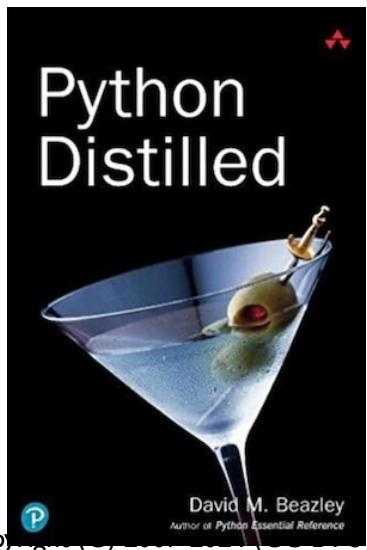
\includegraphics[keepaspectratio]{images/1d2bee38ba6c33cbf76bdd30f1ce96d4f6850b51543f097e737c2643b91fdadd.jpg}}

\pandocbounded{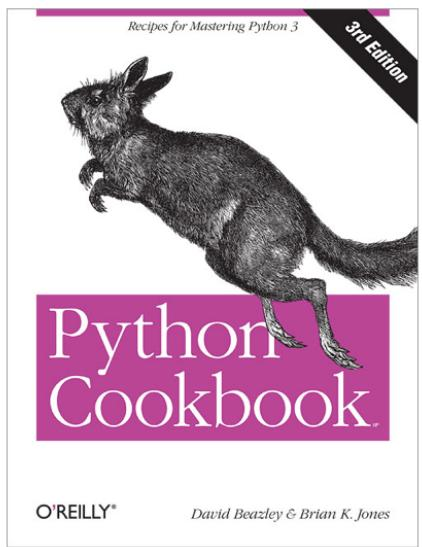
\includegraphics[keepaspectratio]{images/6a063a7118a4552f8b0b5661f24a9a3f0660b16173e11172acce34381f361893.jpg}}

\pandocbounded{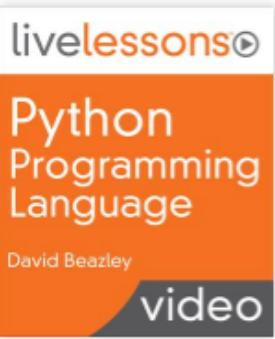
\includegraphics[keepaspectratio]{images/bf09c119d53929b8b820e269135131c81af6ccbb1087ac5f124c0a4b1b0c589c.jpg}}

Python Programming Language 50 reviews by David Beazley

https://www.safaribooksonline.com

\bookmarksetup{startatroot}

\chapter{Course License and Usage}\label{course-license-and-usage}

• Official course materials are here

https://github.com/dabeaz-course/python-mastery

This course is released under the Creative Commons Attribution-Share
Alike 4.0 International (CC-SA 4.0) license.

You are free to use and adapt this material in any way that you wish as
you as you give attribution to the original source. If you choose to use
selected presentation slides in your own course, I kindly ask that the
copyright notice, license, and authorship in the lower-left corner
remain present.

\pandocbounded{
\includegraphics[keepaspectratio]{images/4f45e7285ee69f2116acbee4277a0f0581121589f52487db3565285963d57997.jpg}}

\bookmarksetup{startatroot}

\chapter{About This Course}\label{about-this-course}

Overheard:

``The power of Python grows according to the skill and experience of the
person using it.''

This course is about that!\\
Going far beyond the tutorial\\
Looking at things that you might care about if you're going to write
``real'' programs

\bookmarksetup{startatroot}

\chapter{Target Audience}\label{target-audience}

Programmers who are writing Python code that will be used by others
(libraries, application frameworks, domain-specific languages, etc.)\\
• Topics strongly focus on software development

• Proper usage of Python features\\
Performance tradeoffs\\
Design options

\bookmarksetup{startatroot}

\chapter{System Requirements}\label{system-requirements}

• You should be using Python 3.6 or newer\\
Try to use the latest version\\
• You need a local development environment\\
• Any operating system is fine

\bookmarksetup{startatroot}

\chapter{Prerequisites}\label{prerequisites}

This course assumes that you have already been using Python in some
manner\\
Previously completed some kind of online tutorial, taken an introductory
course, or just worked on some code yourself.\\
You should know the basics of running the interpreter and writing
programs

\bookmarksetup{startatroot}

\chapter{Section 0}\label{section-0}

\bookmarksetup{startatroot}

\chapter{Course Setup}\label{course-setup}

\bookmarksetup{startatroot}

\chapter{Required Files}\label{required-files}

• Where to get Python (if not installed)

http://www.python.org

• This course is written for Python 3.6 or newer\\
• Exercises for this class

github.com/dabeaz-course/python-mastery

• You should clone/fork the repo first

\bookmarksetup{startatroot}

\chapter{Working Environment}\label{working-environment}

• This is not an introductory course\\
• Use whatever tools you currently use to develop Python code\\
Editors, IDEs, etc.\\
• Almost everything in this course is platformneutral and will work
everywhere

\bookmarksetup{startatroot}

\chapter{Class Exercises}\label{class-exercises}

Exercise descriptions are found in

python-mastery/Exercises/

• All exercises have solution code

Write a program that opens this file, reads all lines, int (s ) . To
convert a string to a floating point, use :

\pandocbounded{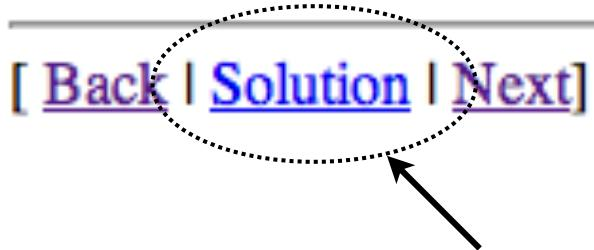
\includegraphics[keepaspectratio]{images/fd15e858e3df5f35ba494d7c4b7bfa89f8621de9d14942a63eda7f2a65cf268e.jpg}}

Look for the link at the bottom!

\bookmarksetup{startatroot}

\chapter{Class Exercises}\label{class-exercises-1}

• Working solution code can be found in

python-mastery/Solutions

• Each problem has its own directory

2\_1/

Exercise 2.1

2\_2/

Exercise 2.2

\bookmarksetup{startatroot}

\chapter{General Tips}\label{general-tips}

• Save all of your work in ``python-mastery''\\
Exercises assume this structure\\
Exercises are meant to be worked in order\\
If stuck, you can often start by copying solution code from Solutions/
and working forward.

\bookmarksetup{startatroot}

\chapter{Section 1}\label{section-1}

\bookmarksetup{startatroot}

\chapter{Python Review}\label{python-review}

(Optional)

\bookmarksetup{startatroot}

\chapter{Overview}\label{overview}

• A very fast-paced review of Python\\
The absolute basics that you should already know if you are taking this
course\\
Essential details for later parts of the class

\bookmarksetup{startatroot}

\chapter{All Things Python}\label{all-things-python}

http://www.python.org

Downloads\\
Documentation and tutorial\\
Community Links\\
• News and more\\
Tutorial

\bookmarksetup{startatroot}

\chapter{Running Python}\label{running-python}

Python programs run inside an interpreter\\
The interpreter is a simple ``console-based'' application that normally
starts from a command shell (e.g., the Unix shell)

\begin{Shaded}
\begin{Highlighting}[]
\NormalTok{bash \% python3  }
\NormalTok{Python 3.6.0 (default, Jan 27 2017, 13:20:23)  }
\NormalTok{[GCC 4.2.1 Compatible Apple LLVM 6.1.0 (clang{-}602.0.53)]  }
\NormalTok{\textgreater{}\textgreater{}\textgreater{} }
\end{Highlighting}
\end{Shaded}

\bookmarksetup{startatroot}

\chapter{Interactive Mode}\label{interactive-mode}

The interpreter runs a ``read-eval'' loop

\begin{Shaded}
\begin{Highlighting}[]
\NormalTok{\textgreater{}\textgreater{}\textgreater{} print(\textquotesingle{}hello world\textquotesingle{})  }
\NormalTok{hello world  }
\NormalTok{\textgreater{}\textgreater{}\textgreater{} 37*42  }
\NormalTok{1554  }
\NormalTok{\textgreater{}\textgreater{}\textgreater{} for i in range(5):  }
\NormalTok{... print(i)  }
\NormalTok{0  }
\NormalTok{1  }
\NormalTok{2  }
\NormalTok{3  }
\NormalTok{4  }
\NormalTok{\textgreater{}\textgreater{}\textgreater{} }
\end{Highlighting}
\end{Shaded}

Executes simple statements typed in directly\\
• Very useful for debugging, exploration

\bookmarksetup{startatroot}

\chapter{Creating Programs}\label{creating-programs}

Programs are put in .py files

\bookmarksetup{startatroot}

\chapter{helloworld.py print(`hello
world')}\label{helloworld.py-printhello-world}

Source files are simple text files\\
• Create with your favorite editor (e.g., emacs)\\
• Make sure you use ``python'' mode

\bookmarksetup{startatroot}

\chapter{Running Programs}\label{running-programs}

\bookmarksetup{startatroot}

\chapter{Command line}\label{command-line}

\begin{Shaded}
\begin{Highlighting}[]
\NormalTok{bash \% python3 helloworld.py  }
\NormalTok{hello world  }
\NormalTok{bash \% }
\end{Highlighting}
\end{Shaded}

\bookmarksetup{startatroot}

\chapter{\#! (Unix)}\label{unix}

\begin{Shaded}
\begin{Highlighting}[]
\NormalTok{!/usr/bin/env python3 \# helloworld.py print(\textquotesingle{}hello world\textquotesingle{}) }
\end{Highlighting}
\end{Shaded}

\bookmarksetup{startatroot}

\chapter{python}\label{python}

• For debugging, use python -i

\begin{Shaded}
\begin{Highlighting}[]
\NormalTok{bash \% python3 {-}i helloworld.py  }
\NormalTok{hello world  }
\NormalTok{\textgreater{}\textgreater{}\textgreater{} }
\end{Highlighting}
\end{Shaded}

Runs your program and then enters the Python interactive shell
afterwards\\
Quite useful for debugging, testing, etc.

\bookmarksetup{startatroot}

\chapter{Exercise}\label{exercise}

Time: 10 minutes

\bookmarksetup{startatroot}

\chapter{Program Execution}\label{program-execution}

• A Python program is a sequence of statements\\
Each statement is terminated by a newline\\
Statements are executed one after the other until you reach the end of
the file.\\
When there are no more statements, the program stops

\bookmarksetup{startatroot}

\chapter{Comments}\label{comments}

Comments are started by \#

\bookmarksetup{startatroot}

\chapter{This is a comment}\label{this-is-a-comment}

height = 442

\bookmarksetup{startatroot}

\chapter{Meters}\label{meters}

• There are no block comments (e.g., /* \ldots{} */).\\
• However, may see ignored code in strings

\bookmarksetup{startatroot}

\chapter{All of this code is ignored}\label{all-of-this-code-is-ignored}

I II

for i in range(10):

print(``Hello'', i)

I II

``Stringy'' code is not a proper comment, but is often a useful trick
when debugging

\bookmarksetup{startatroot}

\chapter{Variables}\label{variables}

• A variable is a name for some value\\
Variable names usually follow same rules as C
{[}A-Za-z\_{]}{[}A-Za-z0-9\_{]}*\\
• You do not declare types (int, float, etc.)

\begin{Shaded}
\begin{Highlighting}[]
\NormalTok{height = 442 \# An integer  }
\NormalTok{height = 442.0 \# Floating point  }
\NormalTok{height = \textquotesingle{}Really tall\textquotesingle{} \# A string }
\end{Highlighting}
\end{Shaded}

Differs from C++/Java where variables have a fixed type that must be
declared.

\bookmarksetup{startatroot}

\chapter{A Bit More on Names}\label{a-bit-more-on-names}

Variable names can actually consist of any Unicode letters and digits.\\
So, writing code like this is valid

\[
\pi = 3. 1 4 1 5 9
\]

\[
\tau = 2 * \pi
\]

However, if it's hard to type on the keyboard or explain, you should
probably avoid it

\bookmarksetup{startatroot}

\chapter{Naming Conventions}\label{naming-conventions}

• Use ``snake case'' for multiple words

\begin{Shaded}
\begin{Highlighting}[]
\NormalTok{first\_name = "Guido"  }
\NormalTok{last\_name = "van Rossum" }
\end{Highlighting}
\end{Shaded}

Prefer lowercase\\
• Use leading \_ for ``private'' names

\begin{Shaded}
\begin{Highlighting}[]
\KeywordTok{def}\NormalTok{ \_\_internal ,( : }
\end{Highlighting}
\end{Shaded}

\bookmarksetup{startatroot}

\chapter{Expressions}\label{expressions}

• Math works normally (precedence, assoc, etc.)

\[
\begin{array}{l} a = 2 + 3 \\ b = 2 + 3 * 4 \\ c = (2 + 3) * 4 \\ \end{array}
\]

Operators are same as C

\[
+, -, *, /, \%, <   <  , > >, \& , |, ^ {\wedge}, \dots
\]

• Other operators (Python-specific)

7 // 4

Truncating division

7 ** 4

Power operator

\bookmarksetup{startatroot}

\chapter{Conditionals}\label{conditionals}

\bookmarksetup{startatroot}

\chapter{If-else}\label{if-else}

if \(a <   b\) print(`Computer says no') else: print(`Computer says
yes')

\bookmarksetup{startatroot}

\chapter{If-elif-else}\label{if-elif-else}

\begin{Shaded}
\begin{Highlighting}[]
\NormalTok{if a == \textquotesingle{} +\textquotesingle{}:  }
\NormalTok{    op = PLUS  }
\NormalTok{elif a == \textquotesingle{}{-}\textquotesingle{}:  }
\NormalTok{    op = MINUS  }
\NormalTok{elif a == \textquotesingle{}*\textquotesingle{}:  }
\NormalTok{    op = TIMES  }
\NormalTok{else:  }
\NormalTok{    op = UNKNOWN }
\end{Highlighting}
\end{Shaded}

\bookmarksetup{startatroot}

\chapter{Relations}\label{relations}

Relational operators

\begin{Shaded}
\begin{Highlighting}[]
\ErrorTok{\textless{}}\NormalTok{ \textgreater{} }\ErrorTok{\textless{}}\NormalTok{= \textgreater{}= == != }
\end{Highlighting}
\end{Shaded}

Boolean expressions (and, or, not)

\begin{Shaded}
\begin{Highlighting}[]
\NormalTok{if b \textgreater{}= a and b \textless{}= c: print(\textquotesingle{}b is between a and c\textquotesingle{})  }
\NormalTok{if not (b \textless{} a or b \textgreater{} c): print(\textquotesingle{}b is still between a and c\textquotesingle{}) }
\end{Highlighting}
\end{Shaded}

\bookmarksetup{startatroot}

\chapter{Looping}\label{looping}

• While statement loops on a condition

while count \(>0\) . print(`T-minus',count) count \(\text{一} = 1\)
print(`Boom!')

For-loop iterates over items (e.g., foreach)

nums = {[}1,7,10,23{]}

for x in nums:

print(x) \# Prints 1, 7, 10, 23

\bookmarksetup{startatroot}

\chapter{Looping Control-Flow}\label{looping-control-flow}

break - terminates a loop early

for name in names: if name == `python': break

continue - skip to next iteration

for line in lines: if line == `\n': \# Ignore blank lines continue

\bookmarksetup{startatroot}

\chapter{Printing}\label{printing}

The print function

print(x) print(x,y,z) print(`Your name is', name)

Produces a single line of text\\
• Items are separated by spaces

\bookmarksetup{startatroot}

\chapter{Formatted Printing}\label{formatted-printing}

f-strings

print(f'\{name:\textgreater10s\} \{shares:\textgreater10d\}
\{price:\textgreater10.2f\}')

• .format() method

print(`\{:10s\} \{:10d\} \{:10.2f\}'.format(name,shares,price))

Use \% operator

print(`\%10s \%10d \%10.2f' \% (name, shares, price))

\bookmarksetup{startatroot}

\chapter{pass statement}\label{pass-statement}

Sometimes you will need to specify an empty block of code

\begin{Shaded}
\begin{Highlighting}[]
\NormalTok{if name in namelist: \# Not implemented yet (or nothing) pass else: statements }
\end{Highlighting}
\end{Shaded}

pass is a ``no-op'' statement\\
It does nothing, but serves as a placeholder for statements (possibly to
be added later)

\bookmarksetup{startatroot}

\chapter{Core Python Objects}\label{core-python-objects}

Programs are built upon a core set of built-in datatypes (numbers,
strings, lists, etc.)

\begin{Shaded}
\begin{Highlighting}[]
\NormalTok{None \# Nothing, nada, nil, ...  }
\NormalTok{True \# Boolean  }
\NormalTok{23 \# Integer  }
\NormalTok{2.3 \# Float  }
\NormalTok{2+3j \# Complex  }
\NormalTok{\textquotesingle{}Hello World\textquotesingle{} \# String (Unicode)  }
\NormalTok{b\textquotesingle{}Hello\textquotesingle{} \# Byte string  }
\NormalTok{(\textquotesingle{}www.python.org\textquotesingle{},80) \# Tuple  }
\NormalTok{[1,2,3,4] \# List  }
\NormalTok{\{\textquotesingle{}name\textquotesingle{}:\textquotesingle{}IBM\textquotesingle{},...\} \# Dictionary }
\end{Highlighting}
\end{Shaded}

You should have already used most of these types if you've written any
Python at all

\bookmarksetup{startatroot}

\chapter{Manipulating Objects}\label{manipulating-objects}

• Objects are manipulated by operators

\begin{Shaded}
\begin{Highlighting}[]
\NormalTok{a + b \# Add  }
\NormalTok{x = a[i] \# Indexed lookup  }
\NormalTok{y = a[i:j] \# Slicing  }
\NormalTok{a[i] = val \# Indexed assignment  }
\NormalTok{x in a \# Containment  }
\NormalTok{... many others ... }
\end{Highlighting}
\end{Shaded}

• Also manipulated by various methods

\begin{Shaded}
\begin{Highlighting}[]
\NormalTok{a.find(}\StringTok{\textquotesingle{}python\textquotesingle{}}\NormalTok{)  }
\NormalTok{a.split([}\StringTok{\textquotesingle{}\textquotesingle{}}\NormalTok{,}\StringTok{\textquotesingle{}])  }
\ErrorTok{b.append}\NormalTok{(}\DecValTok{2}\NormalTok{)  }
\NormalTok{...}
\end{Highlighting}
\end{Shaded}

Available operators/methods depends on the object being manipulated

\bookmarksetup{startatroot}

\chapter{Exercise 1.2}\label{exercise-1.2}

Time: 15 minutes

\bookmarksetup{startatroot}

\chapter{File Input and Output}\label{file-input-and-output}

\bookmarksetup{startatroot}

\chapter{Opening a file}\label{opening-a-file}

\[
f = \text {o p e n} \left(^ {\prime} f o o. t x t ^ {\prime}, ^ {\prime} r ^ {\prime}\right)
\]

\bookmarksetup{startatroot}

\chapter{Open for reading}\label{open-for-reading}

\[
g = \text {o p e n} \left(^ {\prime} b a r. t x t ^ {\prime}, ^ {\prime} w ^ {\prime}\right)
\]

\bookmarksetup{startatroot}

\chapter{Open for writing}\label{open-for-writing}

\[
h = \text {o p e n} \left(^ {\prime} \log . t x t ^ {\prime}, ^ {\prime} a ^ {\prime}\right)
\]

\bookmarksetup{startatroot}

\chapter{Open for appending}\label{open-for-appending}

\bookmarksetup{startatroot}

\chapter{To read data}\label{to-read-data}

\[
\text {l i n e} = \text {f . r e a d l i n e ()}
\]

\bookmarksetup{startatroot}

\chapter{Read a line of text}\label{read-a-line-of-text}

\[
d a t a = f. r e a d ([ m a x b y t e s ])
\]

\bookmarksetup{startatroot}

\chapter{Read data}\label{read-data}

\bookmarksetup{startatroot}

\chapter{To write text to a file}\label{to-write-text-to-a-file}

g.write(`some text')

\bookmarksetup{startatroot}

\chapter{Closing a file (when done)}\label{closing-a-file-when-done}

f.close()

\bookmarksetup{startatroot}

\chapter{Closing Files}\label{closing-files}

Files need to be closed after use

\begin{Shaded}
\begin{Highlighting}[]
\NormalTok{f = open(\textquotesingle{}foo.txt\textquotesingle{}, \textquotesingle{}r\textquotesingle{})}
\NormalTok{\# Use f}
\NormalTok{...}
\NormalTok{f.close() }
\end{Highlighting}
\end{Shaded}

In modern Python, use `with'

\begin{Shaded}
\begin{Highlighting}[]
\ControlFlowTok{with} \BuiltInTok{open}\NormalTok{(}\StringTok{\textquotesingle{}foo.txt\textquotesingle{}}\NormalTok{,}\StringTok{\textquotesingle{}r\textquotesingle{}}\NormalTok{) }\ImportTok{as}\NormalTok{ f: }\CommentTok{\# Use f. \# Automatically closed here }
\end{Highlighting}
\end{Shaded}

\bookmarksetup{startatroot}

\chapter{Common Idioms}\label{common-idioms}

Reading a file line-by-line

with open(`foo.txt',`r') as f: for line in f: \# Process the line

• Reading an entire file into a string

with open(`foo.txt',`r') as f: data \(=\) f.read()

Write to a file

with open(`foo.txt',`w') as f: f.write(`some text\n')

\bookmarksetup{startatroot}

\chapter{Text Data}\label{text-data}

• When reading text, Python 3 assumes unicode\\
• You might need to give an encoding

\[
f = \text {o p e n} \left(^ {\prime} f o o. t x t ^ {\prime}, ^ {\prime} r ^ {\prime}, \text {e n c o d i n g} = ^ {\prime} l a t i n - 1 ^ {\prime}\right)
\]

\bookmarksetup{startatroot}

\chapter{Binary Data}\label{binary-data}

Make sure you use the right file modes if reading binary-encoded data

\[
f = \text {o p e n} \left(^ {\prime} f o o. d a t ^ {\prime}, ^ {\prime} r b ^ {\prime}\right)
\]

\[
g = \text {o p e n} \left(^ {\prime} b a r. b i n ^ {\prime}, ^ {\prime} w b ^ {\prime}\right)
\]

Data read/written to binary-mode files uses normal 8-bit strings\\
Will just have a lot of non-printing control characters, embedded nulls,
etc. for non-text

\bookmarksetup{startatroot}

\chapter{Exercise 1.3}\label{exercise-1.3}

Time: 10 minutes

\bookmarksetup{startatroot}

\chapter{Simple Functions}\label{simple-functions}

• Use functions for code you want to reuse

\begin{Shaded}
\begin{Highlighting}[]
\KeywordTok{def}\NormalTok{ sumcount(n):}
\NormalTok{    total }\OperatorTok{=} \DecValTok{0}
    \ControlFlowTok{while}\NormalTok{ n }\OperatorTok{\textgreater{}} \DecValTok{0}\NormalTok{:}
\NormalTok{        total }\OperatorTok{+=}\NormalTok{ n}
\NormalTok{        n }\OperatorTok{{-}=} \DecValTok{1}
    \ControlFlowTok{return}\NormalTok{ total }
\end{Highlighting}
\end{Shaded}

Calling a function

\begin{Shaded}
\begin{Highlighting}[]
\NormalTok{a = sumcount(100) }
\end{Highlighting}
\end{Shaded}

• A function is just a series of statements that perform some task and
return a result

\bookmarksetup{startatroot}

\chapter{Simple Functions}\label{simple-functions-1}

• Functions behave in a sane manner

Inner variables have local scope\\
Things like recursion work fine\\
• You can have default arguments

Will say more about functions later, but you should already know how to
define and use simple function definitions

\bookmarksetup{startatroot}

\chapter{Exception Handling}\label{exception-handling}

Errors are reported as exceptions\\
• An exception causes the program to stop

\begin{Shaded}
\begin{Highlighting}[]
\NormalTok{\textgreater{}\textgreater{}\textgreater{} int(\textquotesingle{}N/A\textquotesingle{})}
\NormalTok{Traceback (most recent call last):}
\NormalTok{    File "\textless{}stdin\textgreater{}", line 1, in \textless{}module\textgreater{}}
\NormalTok{ValueError: invalid literal for int() with base 10: \textquotesingle{}N/A\textquotesingle{}}
\NormalTok{\textgreater{}\textgreater{}\textgreater{} }
\end{Highlighting}
\end{Shaded}

For debugging, message describes what happened, where the error
occurred, along with a traceback.

\bookmarksetup{startatroot}

\chapter{Exceptions}\label{exceptions}

Exceptions can be caught and handled\\
• To catch, use try-except statement

for line in f: fields \(=\) line.split() try: shares \(=\)
int.fields{[}1{]}) except, ValueError: print(``Couldn't parse'',line)
Name must match the kind of error you're trying to catch \(\ggg\)
int(``N/A'') Traceback (most recent call last): File ``'', line 1, in
ValueError: invalid literal for int(） with base 10:`N/A'
\textgreater\textgreater\textgreater{}

\bookmarksetup{startatroot}

\chapter{Exceptions}\label{exceptions-1}

• To raise an exception, use the raise statement

raise RuntimeError(`What a kerfuffle')

• Will cause the program to abort with an exception traceback (unless
caught by tryexcept)

\% python3 foo.py Traceback (most recent call last): File ``foo.py'',
line 21, in raise RuntimeError(``What a kerfuffle'') RuntimeError: What
a kerfuffle

\bookmarksetup{startatroot}

\chapter{Exception Values}\label{exception-values}

• Most exceptions have an associated value\\
• More information about what's wrong raise RuntimeError(`Invalid user
name')\\
• Passed to variable supplied in except try: except RuntimeError as e:
\ldots{}

• It's an instance of the exception type, but often looks like a string

except RuntimeError as e: print(`Failed : Reason', e)

\bookmarksetup{startatroot}

\chapter{Catching Multiple Errors}\label{catching-multiple-errors}

Can catch different kinds of exceptions try:

except ValueError as e: except TypeError as e:

• Alternatively, if handling is the same

try: except (ValueError, TypeError) as e:

• Catching any exception (danger awaits)

try: except Exception as e:

\bookmarksetup{startatroot}

\chapter{finally statement}\label{finally-statement}

Specifies code that must run regardless of whether or not an exception
occurs

\begin{Shaded}
\begin{Highlighting}[]
\NormalTok{lock }\OperatorTok{=}\NormalTok{ Lock()}
\NormalTok{...}
\NormalTok{lock.acquire()}
\ControlFlowTok{try}\NormalTok{:}
\NormalTok{...}
\ControlFlowTok{finally}\NormalTok{:}
\NormalTok{    lock.release()  }\CommentTok{\# release the lock }
\end{Highlighting}
\end{Shaded}

Commonly use to properly manage resources (especially locks, files,
etc.)

\bookmarksetup{startatroot}

\chapter{Exercise 1.4}\label{exercise-1.4}

Time: 10 minutes

\bookmarksetup{startatroot}

\chapter{Objects}\label{objects}

Python is an object-oriented language\\
All of the basic data types (integers, strings, lists, etc.) are
examples of ``objects''\\
Objects involve data and a set of ``methods'' that carry out various
operations

\begin{Shaded}
\begin{Highlighting}[]
\NormalTok{a }\OperatorTok{=} \StringTok{\textquotesingle{}Hello World\textquotesingle{}} \CommentTok{\# A string object  }
\NormalTok{b }\OperatorTok{=}\NormalTok{ a}\OperatorTok{{-}}\NormalTok{upper() }\CommentTok{\# A method applied to the string  }
\NormalTok{items }\OperatorTok{=}\NormalTok{ [}\DecValTok{1}\NormalTok{,}\DecValTok{2}\NormalTok{,}\DecValTok{3}\NormalTok{] }\CommentTok{\# A list object  }
\NormalTok{items.append(}\DecValTok{4}\NormalTok{) }\CommentTok{\# A method applied to the list }
\end{Highlighting}
\end{Shaded}

\bookmarksetup{startatroot}

\chapter{Classes}\label{classes}

• You can make your own objects

class Player:

\begin{Shaded}
\begin{Highlighting}[]
\KeywordTok{def} \FunctionTok{\_\_init\_\_}\NormalTok{(}\VariableTok{self}\NormalTok{, x, y):}
    \VariableTok{self}\NormalTok{.x }\OperatorTok{=}\NormalTok{ x}
    \VariableTok{self}\NormalTok{.y }\OperatorTok{=}\NormalTok{ y}
    \VariableTok{self}\NormalTok{.health }\OperatorTok{=} \DecValTok{100} 
\end{Highlighting}
\end{Shaded}

\begin{Shaded}
\begin{Highlighting}[]
\KeywordTok{def}\NormalTok{ move(}\VariableTok{self}\NormalTok{, dx, dy): }\VariableTok{self}\NormalTok{.x }\OperatorTok{+=}\NormalTok{ dx }\VariableTok{self}\NormalTok{.y }\OperatorTok{+=}\NormalTok{ dy }
\end{Highlighting}
\end{Shaded}

def damage(self, pts): self.health \(= =\) pts

What is a class?\\
It's all of the function definitions that implement the various methods

\bookmarksetup{startatroot}

\chapter{Instances}\label{instances}

Created by calling the class as a function

\begin{quote}
\begin{quote}
\begin{quote}
a = Player(2, 3)
\end{quote}
\end{quote}
\end{quote}

\begin{quote}
\begin{quote}
\begin{quote}
b = Player(10, 20)
\end{quote}
\end{quote}
\end{quote}

\begin{quote}
\begin{quote}
\begin{quote}
\end{quote}
\end{quote}
\end{quote}

Each instance gets its own data

\begin{Shaded}
\begin{Highlighting}[]
\NormalTok{\textgreater{}\textgreater{}\textgreater{} a.x 2   }
\NormalTok{\textgreater{}\textgreater{}\textgreater{} b.x 10   }
\NormalTok{\textgreater{}\textgreater{}\textgreater{} }
\end{Highlighting}
\end{Shaded}

• Invoke the methods as follows

\begin{Shaded}
\begin{Highlighting}[]
\NormalTok{\textgreater{}\textgreater{}\textgreater{} a}\KeywordTok{.}\NormalTok{move(}\DecValTok{1}\KeywordTok{,} \DecValTok{2}\NormalTok{)  }
\NormalTok{\textgreater{}\textgreater{}\textgreater{} a}\KeywordTok{.}\NormalTok{damage(}\DecValTok{10}\NormalTok{)  }
\NormalTok{\textgreater{}\textgreater{}\textgreater{} }
\end{Highlighting}
\end{Shaded}

\bookmarksetup{startatroot}

\chapter{init method}\label{init-method}

• This method initializes a new instance\\
• Called whenever a new object is created

\begin{Shaded}
\begin{Highlighting}[]
\OperatorTok{\textgreater{}\textgreater{}\textgreater{}}\NormalTok{ a }\OperatorTok{=}\NormalTok{ Player(}\DecValTok{2}\NormalTok{, }\DecValTok{3}\NormalTok{)  }
\KeywordTok{class}\NormalTok{ Player:  }
    \KeywordTok{def} \FunctionTok{\_\_init\_\_}\NormalTok{(}\VariableTok{self}\NormalTok{, x, y):  }
        \VariableTok{self}\NormalTok{.x }\OperatorTok{=}\NormalTok{ x  }
        \VariableTok{self}\NormalTok{.y }\OperatorTok{=}\NormalTok{ y  }
        \VariableTok{self}\NormalTok{.health }\OperatorTok{=} \DecValTok{100}  
\NormalTok{        newly created }\BuiltInTok{object} 
\end{Highlighting}
\end{Shaded}

• Mostly, it just stores the data attributes

\bookmarksetup{startatroot}

\chapter{Methods}\label{methods}

• Functions that operate on instances

class Player:

\begin{Shaded}
\begin{Highlighting}[]
\KeywordTok{def}\NormalTok{ move(}\VariableTok{self}\NormalTok{, dx, dy): }\VariableTok{self}\NormalTok{.x }\OperatorTok{+=}\NormalTok{ dx }\VariableTok{self}\NormalTok{.y }\OperatorTok{+=}\NormalTok{ dy }
\end{Highlighting}
\end{Shaded}

• The object is passed as first argument

\begin{Shaded}
\begin{Highlighting}[]
\OperatorTok{\textgreater{}\textgreater{}\textgreater{}}\NormalTok{ a.move(}\DecValTok{1}\NormalTok{, }\DecValTok{2}\NormalTok{)  }
\KeywordTok{def}\NormalTok{ move(}\VariableTok{self}\NormalTok{, dx, dy): }
\end{Highlighting}
\end{Shaded}

• By convention, the instance is called ``self''

The name is unimportant---the object is always passed as the first
argument. It is simply Python programming style to call this argument
``self.'' It's similar to the ``this'' pointer in C++.

\bookmarksetup{startatroot}

\chapter{Exercise 1.5}\label{exercise-1.5}

Time: 10 minutes

\bookmarksetup{startatroot}

\chapter{Modules}\label{modules}

• Any Python source file is a module

\begin{Shaded}
\begin{Highlighting}[]
\NormalTok{foo.py def grok(a): def spam(b): }
\end{Highlighting}
\end{Shaded}

• import statement loads and executes a module

\begin{Shaded}
\begin{Highlighting}[]
\NormalTok{import foo  }
\NormalTok{a = foo.grok(2)  }
\NormalTok{b = foo.spam(\textquotesingle{}Hello\textquotesingle{})  }
\NormalTok{... }
\end{Highlighting}
\end{Shaded}

\bookmarksetup{startatroot}

\chapter{Namespaces}\label{namespaces}

• A module is a collection of named values (i.e., it's said to be a
``namespace'')\\
The names are simply all of the global variables and functions defined
in the source file\\
• After import, module name used as a prefix

\begin{quote}
\begin{quote}
\begin{quote}
import foo\\
foo.grok(2)
\end{quote}
\end{quote}
\end{quote}

• Module name is tied to source (foo -\textgreater{} foo.py)

\bookmarksetup{startatroot}

\chapter{Globals Revisited}\label{globals-revisited}

Everything defined in the ``global'' scope is what populates the module
namespace

\pandocbounded{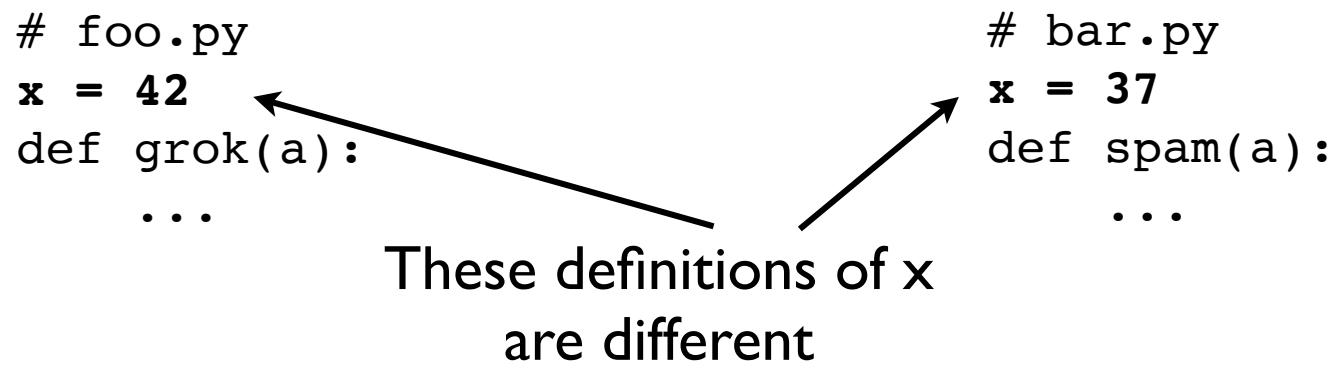
\includegraphics[keepaspectratio]{images/d800860db34264a28bb4cbe91f1fd55c27cb05b3b220017674fb1b02e76adc33.jpg}}

Different modules can use the same names and those names don't conflict
with each other (modules are isolated)

\bookmarksetup{startatroot}

\chapter{import as statement}\label{import-as-statement}

• Changes the local name of a module

\bookmarksetup{startatroot}

\chapter{bar.py import math as m}\label{bar.py-import-math-as-m}

\[
a = m. \sin (x)
\]

Exactly the same as import except the module object is assigned a
different name\\
The new name only applies locally within the source file that did the
import (other files can import using the standard name without any
confusion)

\bookmarksetup{startatroot}

\chapter{from module import}\label{from-module-import}

Lifts selected symbols out of a module and puts them into local scope

\bookmarksetup{startatroot}

\chapter{bar.py from math import
sin,cos}\label{bar.py-from-math-import-sincos}

def rectangular(r,theta): x = r\emph{cos(theta) y = r}sin(theta) return
x,y

Allows parts of a module to be used without having to type the module
prefix

\bookmarksetup{startatroot}

\chapter{from module import *}\label{from-module-import-1}

Takes all symbols from a module and places them into local scope

\begin{Shaded}
\begin{Highlighting}[]
\NormalTok{bar.py from math import \textbackslash{}* }
\end{Highlighting}
\end{Shaded}

\begin{Shaded}
\begin{Highlighting}[]
\KeywordTok{def}\NormalTok{ rectangular(r, theta):}
\NormalTok{    x }\OperatorTok{=}\NormalTok{ r }\OperatorTok{*}\NormalTok{ cos(theta)}
\NormalTok{    y }\OperatorTok{=}\NormalTok{ r }\OperatorTok{*}\NormalTok{ sin(theta)}
    \ControlFlowTok{return}\NormalTok{ x, y }
\end{Highlighting}
\end{Shaded}

Useful if you are going to use a lot of functions from a module and it's
annoying to specify the module prefix all of the time

\bookmarksetup{startatroot}

\chapter{from module import *}\label{from-module-import-2}

You should almost never use it in practice because it leads to poor code
readability\\
Example:

from math import * from random import *

r = gauss(0.0,1.0) \# In what module?

Makes it very difficult to understand someone else's code if you need to
locate the original definition of a library function

\bookmarksetup{startatroot}

\chapter{Main Module}\label{main-module}

Python has no ``main'' function or method\\
Instead, there is a ``main'' module\\
• It's simply the source file that runs first

bash \% python3 foo.py

Whatever module you give to the interpreter at startup becomes ``main''

\bookmarksetup{startatroot}

\chapter{main check}\label{main-check}

It is standard practice for modules that can run as a main program to
use this convention:

foo.py\\
if\_\_name \(\equiv =\) `main'： \#Running as the main program
statements

Statements enclosed inside the if-statement become the ``main'' program

\bookmarksetup{startatroot}

\chapter{Locating Modules}\label{locating-modules}

Modules are loaded from directories on a special module search path
(sys.path)

\begin{Shaded}
\begin{Highlighting}[]
\NormalTok{\textgreater{}\textgreater{}\textgreater{} import sys   }
\NormalTok{\textgreater{}\textgreater{}\textgreater{} sys.path   }
\NormalTok{[\textquotesingle{}\textquotesingle{}, \textquotesingle{}/usr/local/lib/python36.zip\textquotesingle{}， \textquotesingle{}/usr/local/lib/python3.6\textquotesingle{}， \textquotesingle{}/usr/local/lib/python3.6/plat{-}darwin\textquotesingle{}， \textquotesingle{}/usr/local/lib/python3.6/lib{-}dynload\textquotesingle{}，\textquotesingle{}/usr/local/lib/python3.6/site{-}packages\textquotesingle{}]   }
\NormalTok{\textgreater{}\textgreater{}\textgreater{}}
\end{Highlighting}
\end{Shaded}

Most ImportError exceptions are due to issues with the path and/or
filenames

\bookmarksetup{startatroot}

\chapter{Module Search Path}\label{module-search-path}

sys.path contains search path\\
• Can manually adjust if you need to

import sys

sys.path.append(`/project/foo/pyfiles')

Paths also added via environment variables

\% env PYTHONPATH \(\mathbf { \equiv }\) /project/foo/pyfiles python3

Python 3.6.1 (default, Mar 24 2017, 17:58:49)

{[}GCC 4.2.1 Compatible Apple LLVM 8.0.0 (clang-800.0.38){]}

\begin{quote}
\begin{quote}
\begin{quote}
import sys
\end{quote}
\end{quote}
\end{quote}

\begin{quote}
\begin{quote}
\begin{quote}
sys.path
\end{quote}
\end{quote}
\end{quote}

{[}'\,`,'/project/foo/pyfiles', \ldots, {]}

\bookmarksetup{startatroot}

\chapter{Summary}\label{summary}

• This has been an overview of basics\\
If you've already been programming Python for awhile, you should already
know this material\\
• Later sections go into much more depth

\bookmarksetup{startatroot}

\chapter{Exercise 1.6}\label{exercise-1.6}

Time: 5 minutes

\bookmarksetup{startatroot}

\chapter{Section 2}\label{section-2}

\bookmarksetup{startatroot}

\chapter{Data Handling}\label{data-handling}

\bookmarksetup{startatroot}

\chapter{Core Topics}\label{core-topics}

Data structures\\
Containers and collections\\
Iteration\\
Understanding the builtins\\
Object model

\bookmarksetup{startatroot}

\chapter{Data Structures}\label{data-structures}

• Real programs must deal with complex data\\
Example: A holding of stock

100 shares of GOOG at \$490.10

• An ``object'' with three parts

Name (``GOOG'', a string)\\
• Number of shares (100, an integer)\\
Price (490.10, a float)

\bookmarksetup{startatroot}

\chapter{Data Structures}\label{data-structures-1}

Some options

Tuple\\
Dictionary\\
Class instance

• Let's take a short tour

\bookmarksetup{startatroot}

\chapter{Tuples}\label{tuples}

• A collection of values packed together

\[
s = \left(^ {\prime} G O O G ^ {\prime}, 1 0 0, 4 9 0. 1\right)
\]

Can use like an array

\[
\begin{array}{l} \text {n a m e} = \mathbf {s} [ 0 ] \\ \text {c o s t} = \mathbf {s} [ 1 ] * \mathbf {s} [ 2 ] \end{array}
\]

• Unpacking into separate variables

\[
\text {n a m e , s h a r e s , p r i c e} = \mathrm {s}
\]

Immutable

\[
s [ 1 ] = 7 5 \quad \# T y p e R e r r o r. N o i t e m a s s i g n m e n t
\]

\bookmarksetup{startatroot}

\chapter{Dictionaries}\label{dictionaries}

• An unordered set of values indexed by ``keys''

\begin{Shaded}
\begin{Highlighting}[]
\NormalTok{s = \{}
\NormalTok{    \textquotesingle{}name\textquotesingle{} : \textquotesingle{}GOOG\textquotesingle{},}
\NormalTok{    \textquotesingle{}shares\textquotesingle{} : 100,}
\NormalTok{    \textquotesingle{}price\textquotesingle{} : 490.1}
\NormalTok{\} }
\end{Highlighting}
\end{Shaded}

• Use the key name to access

\begin{Shaded}
\begin{Highlighting}[]
\NormalTok{name }\OperatorTok{=}\NormalTok{ s[}\StringTok{\textquotesingle{}name\textquotesingle{}}\NormalTok{]}
\NormalTok{cost }\OperatorTok{=}\NormalTok{ s[}\StringTok{\textquotesingle{}shares\textquotesingle{}}\NormalTok{] }\OperatorTok{*}\NormalTok{ s[}\StringTok{\textquotesingle{}price\textquotesingle{}}\NormalTok{] }
\end{Highlighting}
\end{Shaded}

Modifications are allowed

\begin{Shaded}
\begin{Highlighting}[]
\NormalTok{s[\textquotesingle{}shares\textquotesingle{}] = 75  }
\NormalTok{s[\textquotesingle{}date\textquotesingle{}] = \textquotesingle{}7/25/2015\textquotesingle{}  }
\NormalTok{del s[\textquotesingle{}name\textquotesingle{}] }
\end{Highlighting}
\end{Shaded}

\bookmarksetup{startatroot}

\chapter{User-Defined Classes}\label{user-defined-classes}

\bookmarksetup{startatroot}

\chapter{• A simple data structure
class}\label{a-simple-data-structure-class}

\begin{Shaded}
\begin{Highlighting}[]
\KeywordTok{class}\NormalTok{ Stock: }\KeywordTok{def} \FunctionTok{\_\_init\_\_}\NormalTok{(}\VariableTok{self}\NormalTok{, name, shares, price): }\VariableTok{self}\NormalTok{.name }\OperatorTok{=}\NormalTok{ name }\VariableTok{self}\NormalTok{.share }\OperatorTok{=}\NormalTok{ shares }\VariableTok{self}\NormalTok{.price }\OperatorTok{=}\NormalTok{ price }
\end{Highlighting}
\end{Shaded}

\bookmarksetup{startatroot}

\chapter{• This gives you the nice object
syntax\ldots{}}\label{this-gives-you-the-nice-object-syntax}

\begin{quote}
\begin{quote}
\begin{quote}
s \(\equiv\) Stock(`GOOG'，100，490.1)\\
s.name\\
`GOOG'\\
s.share * s.price\\
49010.0
\end{quote}
\end{quote}
\end{quote}

\bookmarksetup{startatroot}

\chapter{Variations on Classes}\label{variations-on-classes}

• Class definitions have some variants

• Slots - Saves memory\\
• Dataclasses - Reduces coding\\
• Named tuples - Immutability/tuple behavior

Let's take a quick tour

\bookmarksetup{startatroot}

\chapter{Classes and Slots}\label{classes-and-slots}

• For data structures, consider adding \textbf{slots}

\begin{Shaded}
\begin{Highlighting}[]
\KeywordTok{class}\NormalTok{ Stock: }\VariableTok{\_\_slots\_\_} \OperatorTok{=}\NormalTok{ (}\StringTok{\textquotesingle{}name\textquotesingle{}}\NormalTok{, }\StringTok{\textquotesingle{}shares\textquotesingle{}}\NormalTok{, }\StringTok{\textquotesingle{}price\textquotesingle{}}\NormalTok{) }\KeywordTok{def} \FunctionTok{\_\_init\_\_}\NormalTok{(}\VariableTok{self}\NormalTok{, name, shares, price): }\VariableTok{self}\NormalTok{.name }\OperatorTok{=}\NormalTok{ name }\VariableTok{self}\NormalTok{.share }\OperatorTok{=}\NormalTok{ shares }\VariableTok{self}\NormalTok{.price }\OperatorTok{=}\NormalTok{ price }
\end{Highlighting}
\end{Shaded}

Slots is a performance optimization that is specifically aimed at data
structures\\
• Greatly reduces the memory usage

\bookmarksetup{startatroot}

\chapter{Dataclasses}\label{dataclasses}

from dataclasses import dataclass

(\textbf{dataclass?})

class Stock:

name : str

shares : int

price: float

• Possibly a convenience for reducing the amount of code that must be
written\\
• Some useful methods get created automatically\\
However, types are NOT enforced

\bookmarksetup{startatroot}

\chapter{Named Tuples}\label{named-tuples}

• Another variant on class definition

import typing

class Stock(typing.NamedTuple): name: str shares: int price: float

• Alternate formulation (in older code)

from collections import namedtuple

Stock = namedtuple(`Stock', {[}`name', `shares', `price'{]})

Main feature: immutability

\bookmarksetup{startatroot}

\chapter{Named Tuples}\label{named-tuples-1}

Named tuples have same features as tuples (immutability, unpacking,
indexing, etc.)

\begin{quote}
\begin{quote}
\begin{quote}
s = Stock(`GOOG',100,490.1)\\
s{[}0{]} `GOOG'\\
name,shares,price \(=\) s\\
print(`\%10s \%10d \%10.2f' \(\%\) s) GOOG 100 490.10\\
isinstance(s,tuple)\\
True\\
s.name \(=\) `ACME'\\
Traceback (most recent call last) File ``'',line 1,in \textless mod
AttributeError: can't set attribu
\end{quote}
\end{quote}
\end{quote}

\bookmarksetup{startatroot}

\chapter{Exercise 2.1}\label{exercise-2.1}

Time : 30 minutes

\bookmarksetup{startatroot}

\chapter{Containers}\label{containers}

• Programs often have to work many objects

• Lists (ordered data)\\
• Sets (unordered data, no duplicates)\\
Dictionaries (unordered key-value data)

• The choice depends on the problem

\bookmarksetup{startatroot}

\chapter{Lists}\label{lists}

• Use a list when the order of data matters\\
Example: A list of tuples

\begin{Shaded}
\begin{Highlighting}[]
\NormalTok{portfolio }\OperatorTok{=}\NormalTok{ [}
\NormalTok{    (}\StringTok{\textquotesingle{}GOOG\textquotesingle{}}\NormalTok{, }\DecValTok{100}\NormalTok{, }\FloatTok{490.1}\NormalTok{),}
\NormalTok{    (}\StringTok{\textquotesingle{}IBM\textquotesingle{}}\NormalTok{, }\DecValTok{50}\NormalTok{, }\FloatTok{91.1}\NormalTok{),}
\NormalTok{    (}\StringTok{\textquotesingle{}CAT\textquotesingle{}}\NormalTok{, }\DecValTok{150}\NormalTok{, }\FloatTok{83.44}\NormalTok{)}
\NormalTok{] }
\end{Highlighting}
\end{Shaded}

• Lists can be sorted and rearranged

\bookmarksetup{startatroot}

\chapter{Sets}\label{sets}

• A set is an unordered collection of unique items

\[
a = \left\{^ {\prime} I B M ^ {\prime}, ^ {\prime} A A ^ {\prime}, ^ {\prime} A A P L ^ {\prime} \right\}
\]

Sets eliminate duplicates

names = {[}`IBM',`YHOO',`IBM',`CAT',`MSFT',`CAT',`IBM'{]} unique\_names
\(=\) set(names)

Sets are useful for membership tests

members \(=\) set()

members.add(item) \# Add an item members.remove(item) \# Remove an item

if item in members: \# Test for membership \ldots{}

\bookmarksetup{startatroot}

\chapter{Dicts}\label{dicts}

• Useful for indices and lookup tables

prices \(=\) \{ `GOOG' : 513.25, `CAT' : 87.22, `IBM' : 93.37, `MSFT' :
44.12 \}

Common use

\begin{Shaded}
\begin{Highlighting}[]
\NormalTok{p }\OperatorTok{=}\NormalTok{ prices[}\StringTok{\textquotesingle{}IBM\textquotesingle{}}\NormalTok{] }\CommentTok{\# Value lookup  }
\NormalTok{p }\OperatorTok{=}\NormalTok{ prices.get(}\StringTok{\textquotesingle{}AAPL\textquotesingle{}}\NormalTok{, }\FloatTok{0.0}\NormalTok{) }\CommentTok{\# Lookup with default value  }
\NormalTok{prices[}\StringTok{\textquotesingle{}HPE\textquotesingle{}}\NormalTok{] }\OperatorTok{=} \FloatTok{37.42} \CommentTok{\# Assignment  }
\ControlFlowTok{if}\NormalTok{ name }\KeywordTok{in}\NormalTok{ prices: }\CommentTok{\# Membership test }
\end{Highlighting}
\end{Shaded}

\bookmarksetup{startatroot}

\chapter{Dicts, Composite Keys}\label{dicts-composite-keys}

\bookmarksetup{startatroot}

\chapter{• Use tuples for multi-part
keys}\label{use-tuples-for-multi-part-keys}

prices \(=\) \{ (`ACME'，`2017-01-01') : 513.25, (`ACME'，`2017-01-02')
: 512.10, (`ACME'，`2017-01-03') : 512.85, (`SPAM'，`2017-01-01') :
42.1, (`SPAM'，`2017-01-02') : 42.34, (`SPAM'，`2017-01-03') : 42.87, \}

\bookmarksetup{startatroot}

\chapter{Usage:}\label{usage}

\begin{Shaded}
\begin{Highlighting}[]
\NormalTok{p }\OperatorTok{=}\NormalTok{ prices[}\StringTok{\textquotesingle{}ACME\textquotesingle{}}\NormalTok{, }\StringTok{\textquotesingle{}2017{-}01{-}01\textquotesingle{}}\NormalTok{]}
\NormalTok{prices[}\StringTok{\textquotesingle{}ACME\textquotesingle{}}\NormalTok{, }\StringTok{\textquotesingle{}2017{-}01{-}04\textquotesingle{}}\NormalTok{] }\OperatorTok{=} \FloatTok{515.20} 
\end{Highlighting}
\end{Shaded}

\bookmarksetup{startatroot}

\chapter{Comprehensions}\label{comprehensions}

List comprehension

{[} expression for item in sequence if condition {]}

Set comprehension

\{ expression for item in sequence if condition \}

Dict comprehension

\{ key:value for item in sequence if condition \}

These often simplify the creation of lists, sets, and dictionaries from
existing data

\bookmarksetup{startatroot}

\chapter{Comprehensions}\label{comprehensions-1}

General syntax

{[}expression for item in sequence if condition{]}

What it means

result \(=\) {[}{]}\\
for item in sequence: if condition: result.append(expression)

Similar for set and dict comprehensions

\bookmarksetup{startatroot}

\chapter{Comprehension Examples}\label{comprehension-examples}

Collecting values from data

names = {[}s{[}`name'{]} for s in portfolio{]}

Unique values

unique\_names = \{s{[}`name'{]} for s in portfolio\}

Performing database-like queries

results = {[}s for s in portfolio if s{[}`price'{]} \textgreater{} 100
and s{[}`shares'{]} \textgreater{} 50 {]}

• Quick mathematics over sequences

cost \(=\) sum({[}s{[}`shares'{]}*s{[}`price'{]} for s in portfolio{]})

\bookmarksetup{startatroot}

\chapter{Collections Module}\label{collections-module}

Provides some variations on common data structures (useful for
specialized problems)

defaultdict\\
Counter\\
deque\\
\ldots{} and more

\bookmarksetup{startatroot}

\chapter{defaultdict}\label{defaultdict}

\bookmarksetup{startatroot}

\chapter{• Automatic initialization of missing dict
keys}\label{automatic-initialization-of-missing-dict-keys}

from collections import defaultdict

\begin{quote}
\begin{quote}
\begin{quote}
d \(=\) defaultdict(list)\\
d\\
defaultdict(\textless class `list'\textgreater，\{\}）\\
d{[}`x'{]}\\
{[}{]}\\
d\\
defaultdict(\textless class `list'\textgreater，\{`x'：{[}{]}\})
\end{quote}
\end{quote}
\end{quote}

\bookmarksetup{startatroot}

\chapter{• Allows combined operations}\label{allows-combined-operations}

\begin{Shaded}
\begin{Highlighting}[]
\NormalTok{\textgreater{}\textgreater{}\textgreater{}d[\textquotesingle{}y\textquotesingle{}].append(42)   }
\NormalTok{\textgreater{}\textgreater{}\textgreater{}d[\textquotesingle{}y\textquotesingle{}]   }
\NormalTok{[42]   }
\NormalTok{\textgreater{}\textgreater{}\textgreater{} }
\end{Highlighting}
\end{Shaded}

\bookmarksetup{startatroot}

\chapter{Counter}\label{counter}

• A dictionary specialized for counting items

from collections import Counter

\begin{quote}
\begin{quote}
\begin{quote}
totals \(=\) Counter()\\
totals{[}`IBM'{]} += 20\\
totals{[}`AA'{]} += 50\\
totals{[}`ACME'{]} += 75\\
totals
\end{quote}
\end{quote}
\end{quote}

Counter(\{`ACME': 75, `AA': 50, `IBM': 20\})

\begin{quote}
\begin{quote}
\begin{quote}
\end{quote}
\end{quote}
\end{quote}

• Has some other nice features (i.e., ranking)

\begin{quote}
\begin{quote}
\begin{quote}
totals.most\_common(2)
\end{quote}
\end{quote}
\end{quote}

{[}(`ACME', 75), (`AA', 50){]}

\begin{quote}
\begin{quote}
\begin{quote}
\end{quote}
\end{quote}
\end{quote}

\bookmarksetup{startatroot}

\chapter{deque}\label{deque}

\bookmarksetup{startatroot}

\chapter{Double-ended queue}\label{double-ended-queue}

from collections import deque

\begin{quote}
\begin{quote}
\begin{quote}
q = deque()\\
q.append(1)\\
q.append(2)\\
q.appendleft(3)\\
q.appendleft(4)\\
q
\end{quote}
\end{quote}
\end{quote}

deque({[}4, 3, 1, 2{]})\\
\textgreater\textgreater\textgreater{} q.pop()\\
2\\
\textgreater\textgreater\textgreater{} q.popleft()\\
4\\
\textgreater\textgreater\textgreater{}

• More efficient than a list for queuing problems

\bookmarksetup{startatroot}

\chapter{Keeping a History}\label{keeping-a-history}

• Problem: Keep a history of the last N things

\begin{Shaded}
\begin{Highlighting}[]
\NormalTok{line1 line2 }
\end{Highlighting}
\end{Shaded}

\begin{Shaded}
\begin{Highlighting}[]
\NormalTok{line3 line4 line5 }
\end{Highlighting}
\end{Shaded}

\begin{Shaded}
\begin{Highlighting}[]
\NormalTok{history = [ line3, line4, line5 ] }
\end{Highlighting}
\end{Shaded}

Solution: Use a deque

from collections import deque

history \(=\) deque(maxlen \(\equiv\) N)\\
with open(FILEname) as f: for line in f: history.append(line)

\bookmarksetup{startatroot}

\chapter{Multi-Search}\label{multi-search}

\bookmarksetup{startatroot}

\chapter{Problem: Search multiple
places}\label{problem-search-multiple-places}

techs \(=\) \{ auto \(\equiv\) \{ IBM':91.23, `GM':23.45, `AAPL':123.45,
`TM':87.20, HPE':34.23 F':51.1, \} `TTA':64.45, \}

\bookmarksetup{startatroot}

\chapter{Solution: ChainMap}\label{solution-chainmap}

from collections import ChainMap allprices \(=\) ChainMap(techs, auto)

\begin{Shaded}
\begin{Highlighting}[]
\NormalTok{\textgreater{}\textgreater{}\textgreater{} allprices[\textquotesingle{}HPE\textquotesingle{}] 34.23   }
\NormalTok{\textgreater{}\textgreater{}\textgreater{} allprices[\textquotesingle{}F\textquotesingle{}] 51.1   }
\NormalTok{\textgreater{}\textgreater{}\textgreater{} }
\end{Highlighting}
\end{Shaded}

\bookmarksetup{startatroot}

\chapter{Commentary}\label{commentary}

• collections is a useful module to know\\
• Simplifies many common data handling problems\\
• If you're not using it, you're missing out

\bookmarksetup{startatroot}

\chapter{Exercise 2.2}\label{exercise-2.2}

Time : 45 minutes

\bookmarksetup{startatroot}

\chapter{Iteration}\label{iteration}

The for-loop iterates over a sequence

\begin{quote}
\begin{quote}
\begin{quote}
names \(=\) {[}`IBM'，`YHOO'，`AA'，`CAT'{]}\\
for name in names: print(name)\\
IBM\\
YHOO\\
AA\\
CAT
\end{quote}
\end{quote}
\end{quote}

It seems simple enough\ldots{}

\bookmarksetup{startatroot}

\chapter{Iterating on Tuples}\label{iterating-on-tuples}

\bookmarksetup{startatroot}

\chapter{Consider a list of tuples}\label{consider-a-list-of-tuples}

portfolio \(=\) {[} (`GOOG',100,490.1), (`IBM',50,91.1),
(`CAT',150,83.44), (`IBM',100,45.23), (`GOOG',75,572.45),
(`AA',50,23.15){]}

\bookmarksetup{startatroot}

\chapter{Iteration with unpacking}\label{iteration-with-unpacking}

for name, shares, price in portfolio:

\bookmarksetup{startatroot}

\chapter{Iteration with a ``throwaway'' value (use
\_)}\label{iteration-with-a-throwaway-value-use-_}

for name, \_, price in portfolio: ..

\bookmarksetup{startatroot}

\chapter{Iterating on Varying
Records}\label{iterating-on-varying-records}

• Consider a list of varying sized data structures

prices \(=\) {[} {[}`GOOG',490.1,485.25，487.5{]}， {[}`IBM'，91.5{]}，
{[}`HPE'，13.75，12.1，13.25，14.2，13.5{]}， {[}`CAT'，52.5，51.2{]}
{]}

• Wildcard unpacking (Python 3 only)

for name, *values in prices: print(name, values)

\begin{Shaded}
\begin{Highlighting}[]
\NormalTok{name values  }
\NormalTok{\textquotesingle{}GOOG\textquotesingle{} [490.1, 485.25, 487.5]  }
\NormalTok{\textquotesingle{}IBM\textquotesingle{} [91.5]  }
\NormalTok{\textquotesingle{}HPE\textquotesingle{} [13.75, 12.1, 13.25, 14.2, 13.5]  }
\NormalTok{\textquotesingle{}CAT\textquotesingle{} [52.5, 51.2] }
\end{Highlighting}
\end{Shaded}

\bookmarksetup{startatroot}

\chapter{zip() function}\label{zip-function}

Iterate on multiple sequences in parallel

columns = {[}`name',`shares',`price'{]}

values = {[}`GOOG',100, 490.1 {]}

for colname, val in zip(columns, values):

\bookmarksetup{startatroot}

\chapter{\texorpdfstring{Loops with colname \(=\) `name'
val=`GOOG'}{Loops with colname = `name' val=`GOOG'}}\label{loops-with-colname-name-valgoog}

\bookmarksetup{startatroot}

\chapter{\texorpdfstring{colname \({ } = { }\) `shares'
\(\mathtt { v a l } { = } 1 0 0\)}{colname \{ \} = \{ \} `shares' \textbackslash mathtt \{ v a l \} \{ = \} 1 0 0}}\label{colname-shares-mathtt-v-a-l-1-0-0}

\bookmarksetup{startatroot}

\chapter{\texorpdfstring{colname \(=\) `price'
val=490.1}{colname = `price' val=490.1}}\label{colname-price-val490.1}

Common use: Making dictionaries

record \(=\) dict(zip(columns,values))

Caution: Truncates to shortest input length

zip({[}`a',`b',`c'{]}, {[}1,2{]}) (`a', 1), (`b', 2)

\bookmarksetup{startatroot}

\chapter{Keeping a Running Count}\label{keeping-a-running-count}

enumerate(sequence {[}, start{]})

\begin{Shaded}
\begin{Highlighting}[]
\NormalTok{names }\OperatorTok{=}\NormalTok{ [}\StringTok{\textquotesingle{}IBM\textquotesingle{}}\NormalTok{, }\StringTok{\textquotesingle{}YHOO\textquotesingle{}}\NormalTok{, }\StringTok{\textquotesingle{}CAT\textquotesingle{}}\NormalTok{]  }
\ControlFlowTok{for}\NormalTok{ n, name }\KeywordTok{in} \BuiltInTok{enumerate}\NormalTok{ names)  }
    \CommentTok{\# Loops with n=0 name=\textquotesingle{}IBM\textquotesingle{}  }
    \CommentTok{\# n=1 name=\textquotesingle{}YHOO\textquotesingle{}  }
    \CommentTok{\# n=2 name=\textquotesingle{}CAT\textquotesingle{} }
\end{Highlighting}
\end{Shaded}

Example: Line number tracking on a file

\begin{Shaded}
\begin{Highlighting}[]
\NormalTok{with open(filename) as f: for lineno, line in enumerate(f, start=1): }
\end{Highlighting}
\end{Shaded}

\bookmarksetup{startatroot}

\chapter{Iterating on Integers}\label{iterating-on-integers}

range({[}start,{]} end {[},step{]})

for i in range(100):

\bookmarksetup{startatroot}

\chapter{i = 0,1,\ldots,99}\label{i-0199}

for j in range(10,20):

\bookmarksetup{startatroot}

\chapter{j = 10,11,\ldots, 19}\label{j-1011-19}

for k in range(10,50,2):

\bookmarksetup{startatroot}

\chapter{k = 10,12,\ldots,48}\label{k-101248}

• Note: The ending value is never included\\
Caution: range() is often a ``code smell'' for problems being solved the
``hard way''

\bookmarksetup{startatroot}

\chapter{Sequence Reductions}\label{sequence-reductions}

sum(s), min(s), max(s)

\begin{quote}
\begin{quote}
\begin{quote}
s = {[}1, 2, 3, 4{]}
\end{quote}
\end{quote}
\end{quote}

\begin{quote}
\begin{quote}
\begin{quote}
sum(s)
\end{quote}
\end{quote}
\end{quote}

10

\begin{quote}
\begin{quote}
\begin{quote}
min(s)
\end{quote}
\end{quote}
\end{quote}

1

\begin{quote}
\begin{quote}
\begin{quote}
max(s)
\end{quote}
\end{quote}
\end{quote}

4

\begin{quote}
\begin{quote}
\begin{quote}
\end{quote}
\end{quote}
\end{quote}

Boolean tests: any(s), all(s)

\begin{quote}
\begin{quote}
\begin{quote}
s = {[}False, True, True, False{]}
\end{quote}
\end{quote}
\end{quote}

\begin{quote}
\begin{quote}
\begin{quote}
any(s)
\end{quote}
\end{quote}
\end{quote}

True

\begin{quote}
\begin{quote}
\begin{quote}
all(s)
\end{quote}
\end{quote}
\end{quote}

False

\begin{quote}
\begin{quote}
\begin{quote}
\end{quote}
\end{quote}
\end{quote}

\bookmarksetup{startatroot}

\chapter{Unpacking Iterables}\label{unpacking-iterables}

Consider these iterables

\[
\begin{array}{l} a = (1, 2, 3) \\ b = [ 4, 5 ] \\ \end{array}
\]

• Making lists and tuples (Python 3.5+)

\[
\begin{array}{l} c = [ * a, * b ] \quad \# c = [ 1, 2, 3, 4, 5 ] \quad (l i s t) \\ d = \left( \begin{array}{l l} * a, & * b \end{array} \right) \quad \# d = (1, 2, 3, 4, 5) \quad (t u p l e) \\ \end{array}
\]

• It's subtle, but maybe better than using +

\[
\gg \gg c = a + b
\]

Traceback (most recent call last):

File ``'', line 1, in

TypeError: can only concatenate tuple (not ``list'') to tuple
\textgreater\textgreater\textgreater{}

\bookmarksetup{startatroot}

\chapter{Unpacking Dictionaries}\label{unpacking-dictionaries}

\bookmarksetup{startatroot}

\chapter{Consider these dicts}\label{consider-these-dicts}

\begin{Shaded}
\begin{Highlighting}[]
\NormalTok{a }\OperatorTok{=}\NormalTok{ \{}\StringTok{\textquotesingle{}name\textquotesingle{}}\NormalTok{: }\StringTok{\textquotesingle{}GOOG\textquotesingle{}}\NormalTok{, }\StringTok{\textquotesingle{}shares\textquotesingle{}}\NormalTok{: }\DecValTok{100}\NormalTok{, }\StringTok{\textquotesingle{}price\textquotesingle{}}\NormalTok{: }\FloatTok{490.1}\NormalTok{\}  }
\NormalTok{b }\OperatorTok{=}\NormalTok{ \{}\StringTok{\textquotesingle{}date\textquotesingle{}}\NormalTok{: }\StringTok{\textquotesingle{}6/11/2007\textquotesingle{}}\NormalTok{, }\StringTok{\textquotesingle{}time\textquotesingle{}}\NormalTok{: }\StringTok{\textquotesingle{}9:45am\textquotesingle{}}\NormalTok{\} }
\end{Highlighting}
\end{Shaded}

\bookmarksetup{startatroot}

\chapter{• Combining into a single dict (Python
3.5+)}\label{combining-into-a-single-dict-python-3.5}

\(\mathbf{c} = \{\text{**a}, \text{**b}\}\)
\textgreater\textgreater\textgreater{} c\\
\{ `name': `GOOG', `shares': 100, `price': 490.1, `date': `6/11/2007',
`time': `9:45am' \}\\
\textgreater\textgreater\textgreater{}

\bookmarksetup{startatroot}

\chapter{Argument Passing}\label{argument-passing}

Iterables can expand to positional args

\[
\begin{array}{l} a = (1, 2, 3) \\ b = (4, 5) \\ \end{array}
\]

func(\emph{a, }b) \# func(1,2,3,4,5)

• Dictionaries can expand to keyword args

\[
c = \left\{^ {\prime} x ^ {\prime}: 1, ^ {\prime} y ^ {\prime}: 2 \right\}
\]

func(**c) func(x=1, y=2)

Combinations fine as long as positional go first

func(*a, **c)

func(\emph{a, }b, **c)

func(0, \emph{a, }b, 6, spam=37, **c)

\bookmarksetup{startatroot}

\chapter{Generator Expressions}\label{generator-expressions}

• A variant of a list comprehension that produces the results via
iteration\\
• Slightly different syntax (parentheses)

\[
\begin{array}{l} \text {n u m s} = [ 1, 2, 3, 4 ] \\ \text {s q u a r e s} = (\mathrm {x} ^ {*} \mathrm {x} \text {f o r x i n n u m s}) \end{array}
\]

• Use iteration to get the results

for n in squares:

\bookmarksetup{startatroot}

\chapter{Generators}\label{generators}

• A generator can only be consumed once\\
Example:

\begin{Shaded}
\begin{Highlighting}[]
\NormalTok{\textgreater{}\textgreater{}\textgreater{} nums }\KeywordTok{=}\NormalTok{ [}\DecValTok{1}\NormalTok{,}\DecValTok{2}\NormalTok{,}\DecValTok{3}\NormalTok{,}\DecValTok{4}\NormalTok{]  }
\NormalTok{\textgreater{}\textgreater{}\textgreater{} squares }\KeywordTok{=}\NormalTok{ (x}\FunctionTok{*}\NormalTok{x for x in nums)  }
\NormalTok{\textgreater{}\textgreater{}\textgreater{} for n in squares}\FunctionTok{:}  
\NormalTok{    print(n}\KeywordTok{,}\NormalTok{ end}\KeywordTok{=}\StringTok{\textquotesingle{}\textquotesingle{}}\NormalTok{)  }
\DecValTok{1} \DecValTok{4} \DecValTok{9} \DecValTok{16}  
\NormalTok{\textgreater{}\textgreater{}\textgreater{} for n in squares}\FunctionTok{:}  
\NormalTok{    print(n}\KeywordTok{,}\NormalTok{ end}\KeywordTok{=}\StringTok{\textquotesingle{}\textquotesingle{}}\NormalTok{)  }
\ErrorTok{←}\NormalTok{ notice no output (spent)  }
\NormalTok{\textgreater{}\textgreater{}\textgreater{} }
\end{Highlighting}
\end{Shaded}

\bookmarksetup{startatroot}

\chapter{Using Generators}\label{using-generators}

Generators are useful in contexts where the result is an intermediate
step\\
• For example:

\begin{Shaded}
\begin{Highlighting}[]
\KeywordTok{def}\NormalTok{ sumsquares(nums):}
\NormalTok{    squares }\OperatorTok{=}\NormalTok{ (x }\OperatorTok{*}\NormalTok{ x }\ControlFlowTok{for}\NormalTok{ x }\KeywordTok{in}\NormalTok{ nums)}
\NormalTok{    total }\OperatorTok{=} \BuiltInTok{sum}\NormalTok{(squares)}
    \ControlFlowTok{return}\NormalTok{ total }
\end{Highlighting}
\end{Shaded}

Observe: squares is a temporary value-- no need to make a list

\bookmarksetup{startatroot}

\chapter{Generator Arguments}\label{generator-arguments}

Generators expressions are sometimes embedded as a function argument

sum( \(\mathbf { x } \star \mathbf { x }\) for x in nums)

print(`,'.join(str(x) for x in items))

if any(name.endswith(`.py') for name in filenames): \ldots{}

• It acts as a filter/transform on an iterable

sum(x*x for x in nums)

\pandocbounded{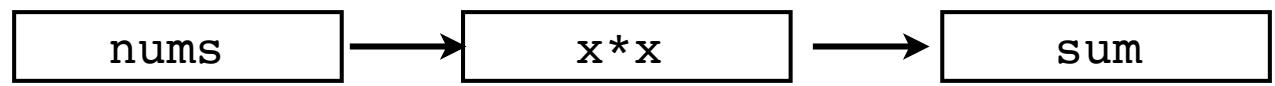
\includegraphics[keepaspectratio]{images/0445dccbb52c1a4ab3a6bc9c90b588daabb6c6e74b9cf567adf9ad669fdef6e0.jpg}}

\bookmarksetup{startatroot}

\chapter{Generator Functions}\label{generator-functions}

• A function that feeds iteration

def squares(nums): for x in nums: yield \(x^{*}x\) \# Emit a value

• To get the results, use iteration

\begin{Shaded}
\begin{Highlighting}[]
\NormalTok{for n in squares([1,2,3,4]): }
\end{Highlighting}
\end{Shaded}

This a more general form that can be used if the iteration processing is
more complicated

\bookmarksetup{startatroot}

\chapter{Exercise 2.3}\label{exercise-2.3}

Time : 10 minutes

\bookmarksetup{startatroot}

\chapter{Secrets of the Builtins}\label{secrets-of-the-builtins}

Programmers use the built-in types without giving them much thought\\
However, they have some subtle behavior that is worth knowing about\\
Especially if you want to write better code

\bookmarksetup{startatroot}

\chapter{What is a Builtin?}\label{what-is-a-builtin}

• An object that's part of the Python interpreter\\
• Usually implemented entirely in C\\
In some sense, the most primitive kind of object that you can use in a
program

\bookmarksetup{startatroot}

\chapter{Under the Hood}\label{under-the-hood}

• All objects have an id, class and a reference count

\pandocbounded{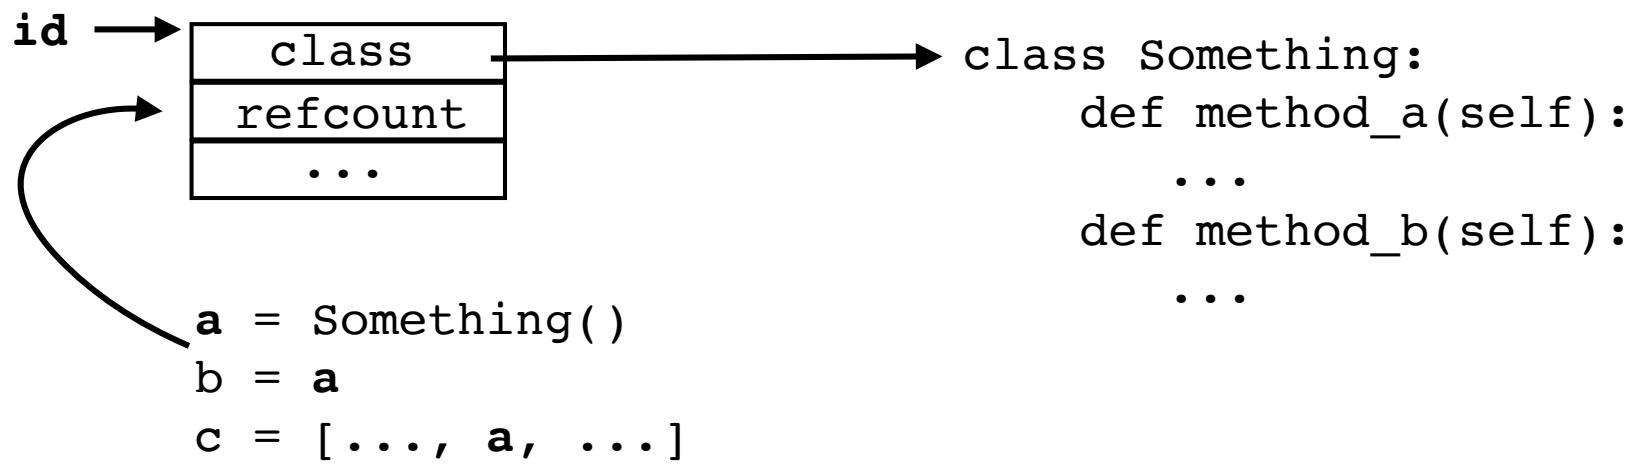
\includegraphics[keepaspectratio]{images/7e2e82d973644c7e2c159eee499d6bd52fd719641c197b99bc013bf637493f61.jpg}}

• The id is the memory address\\
The class is the ``type''\\
• Reference count used for garbage collection

\bookmarksetup{startatroot}

\chapter{Builtin Representation}\label{builtin-representation}

• None (a singleton)

class

refcount

(16 bytes)

float (64-bit double precision)

class

refcount

value

(24 bytes)

int (arbitrary precision)

class

refcount

size

digits

···

digits

(28-??? bytes)

digits stored in 30-bit chunks

\bookmarksetup{startatroot}

\chapter{String Representation}\label{string-representation}

\begin{Shaded}
\begin{Highlighting}[]
\NormalTok{class refcount length hash flags meta data }
\end{Highlighting}
\end{Shaded}

• Strings adapt to Unicode (size may vary)

\begin{Shaded}
\begin{Highlighting}[]
\NormalTok{\textgreater{}\textgreater{}\textgreater{} a = \textquotesingle{}n\textquotesingle{} }
\end{Highlighting}
\end{Shaded}

\begin{Shaded}
\begin{Highlighting}[]
\NormalTok{\textgreater{}\textgreater{}\textgreater{} b = \textquotesingle{}til\textquotesingle{} }
\end{Highlighting}
\end{Shaded}

\begin{Shaded}
\begin{Highlighting}[]
\NormalTok{\textgreater{}\textgreater{}\textgreater{} sys.getsizeof(a) }
\end{Highlighting}
\end{Shaded}

\begin{Shaded}
\begin{Highlighting}[]
\NormalTok{50 }
\end{Highlighting}
\end{Shaded}

\begin{Shaded}
\begin{Highlighting}[]
\NormalTok{\textgreater{}\textgreater{}\textgreater{} sys.getsizeof(b) }
\end{Highlighting}
\end{Shaded}

\begin{Shaded}
\begin{Highlighting}[]
\NormalTok{74 }
\end{Highlighting}
\end{Shaded}

\begin{Shaded}
\begin{Highlighting}[]
\NormalTok{\textgreater{}\textgreater{}\textgreater{} }
\end{Highlighting}
\end{Shaded}

\bookmarksetup{startatroot}

\chapter{Memory Overhead}\label{memory-overhead}

• There is inherent memory overhead\\
• Can investigate with sys.getsizeof()

\begin{Shaded}
\begin{Highlighting}[]
\NormalTok{\textgreater{}\textgreater{}\textgreater{} import sys  }
\NormalTok{\textgreater{}\textgreater{}\textgreater{} a = 2  }
\NormalTok{\textgreater{}\textgreater{}\textgreater{} sys.getsizeof(a)  }
\NormalTok{28  }
\NormalTok{\textgreater{}\textgreater{}\textgreater{} b = 2.5  }
\NormalTok{\textgreater{}\textgreater{}\textgreater{} sys.getsizeof(b)  }
\NormalTok{24  }
\NormalTok{\textgreater{}\textgreater{}\textgreater{} c = \textquotesingle{}2.5\textquotesingle{}  }
\NormalTok{\textgreater{}\textgreater{}\textgreater{} sys.getsizeof(c)  }
\NormalTok{52  }
\NormalTok{\textgreater{}\textgreater{}\textgreater{} }
\end{Highlighting}
\end{Shaded}

• A big part of memory use in earlier exercises

\bookmarksetup{startatroot}

\chapter{Operation of the Builtins}\label{operation-of-the-builtins}

The builtin types operate according to predefined ``protocols'' (special
methods)

\begin{Shaded}
\begin{Highlighting}[]
\NormalTok{\textgreater{}\textgreater{}\textgreater{} a = 2  }
\NormalTok{\textgreater{}\textgreater{}\textgreater{} b = 3  }
\NormalTok{\textgreater{}\textgreater{}\textgreater{} a + b  }
\NormalTok{5  }
\NormalTok{\textgreater{}\textgreater{}\textgreater{} a.\_add\_\_(b) \# Protocol  }
\NormalTok{5  }
\NormalTok{\textgreater{}\textgreater{}\textgreater{} c = \textquotesingle{}hello\textquotesingle{}  }
\NormalTok{\textgreater{}\textgreater{}\textgreater{} len(c)  }
\NormalTok{5  }
\NormalTok{\textgreater{}\textgreater{}\textgreater{} c.\_len\_( ) \# Protocol  }
\NormalTok{5 }
\end{Highlighting}
\end{Shaded}

\bookmarksetup{startatroot}

\chapter{Object Protocols}\label{object-protocols}

The object protocols are baked into the interpreter at a very low level
(byte code)

\begin{Shaded}
\begin{Highlighting}[]
\OperatorTok{\textgreater{}\textgreater{}\textgreater{}} \KeywordTok{def}\NormalTok{ f(x, y): }\ControlFlowTok{return}\NormalTok{ x }\OperatorTok{+}\NormalTok{ y  }
\OperatorTok{\textgreater{}\textgreater{}\textgreater{}} \ImportTok{import}\NormalTok{ dis  }
\OperatorTok{\textgreater{}\textgreater{}\textgreater{}}\NormalTok{ dis.dis(f)  }
\DecValTok{2} \DecValTok{0}\NormalTok{ LOAD }
\end{Highlighting}
\end{Shaded}

\pandocbounded{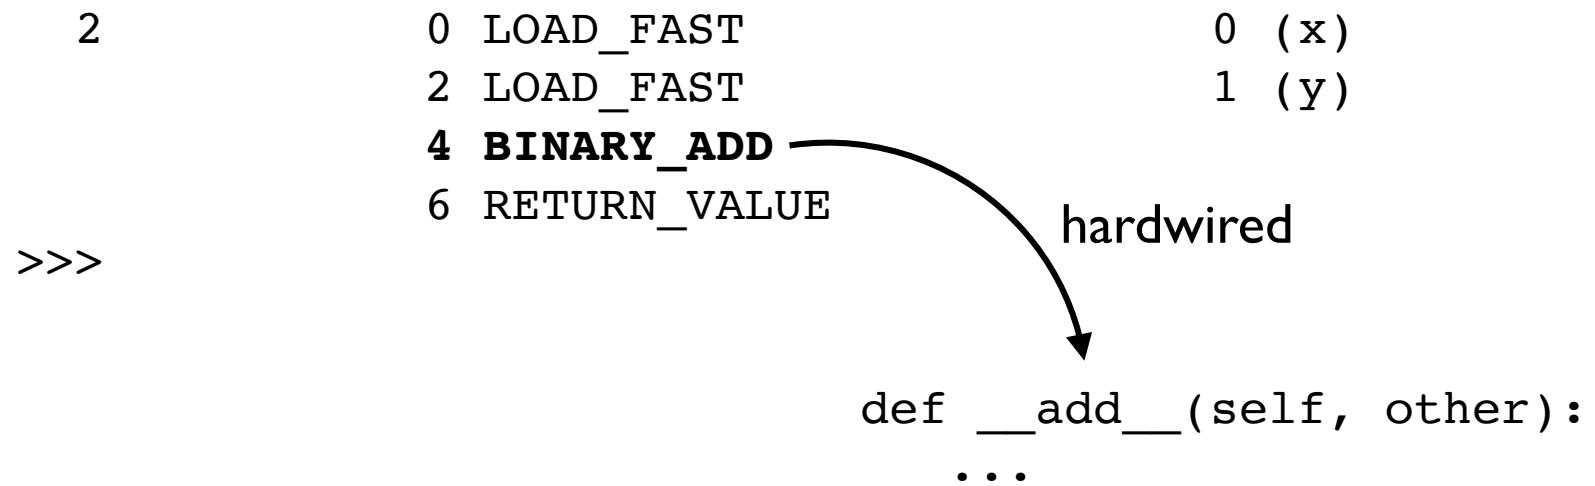
\includegraphics[keepaspectratio]{images/df2ac93ed74f26c9af91b0f5e9a648393f4d76d1ca7e585d9f4a94f07b136257.jpg}}

\bookmarksetup{startatroot}

\chapter{Making New ``Builtins''}\label{making-new-builtins}

Awareness of protocols allows you to make new objects that behave like
the builtins\\
Example: decimals, fractions

\begin{Shaded}
\begin{Highlighting}[]
\OperatorTok{\textgreater{}\textgreater{}\textgreater{}} \ImportTok{from}\NormalTok{ fractions }\ImportTok{import}\NormalTok{ Fraction  }
\OperatorTok{\textgreater{}\textgreater{}\textgreater{}}\NormalTok{ a }\OperatorTok{=}\NormalTok{ Fraction(}\DecValTok{2}\NormalTok{, }\DecValTok{3}\NormalTok{)  }
\OperatorTok{\textgreater{}\textgreater{}\textgreater{}}\NormalTok{ b }\OperatorTok{=}\NormalTok{ Fraction(}\DecValTok{1}\NormalTok{, }\DecValTok{2}\NormalTok{)  }
\OperatorTok{\textgreater{}\textgreater{}\textgreater{}}\NormalTok{ a }\OperatorTok{+}\NormalTok{ b  }
\NormalTok{Fraction(}\DecValTok{7}\NormalTok{, }\DecValTok{6}\NormalTok{)  }
\OperatorTok{\textgreater{}\textgreater{}\textgreater{}}\NormalTok{ a }\OperatorTok{\textgreater{}} \FloatTok{0.5}  
\VariableTok{True} 
\end{Highlighting}
\end{Shaded}

\bookmarksetup{startatroot}

\chapter{Exercise 2.4}\label{exercise-2.4}

Time : 30 Minutes

\bookmarksetup{startatroot}

\chapter{Container Representation}\label{container-representation}

• Container objects only hold references (pointers) to their stored
values

\pandocbounded{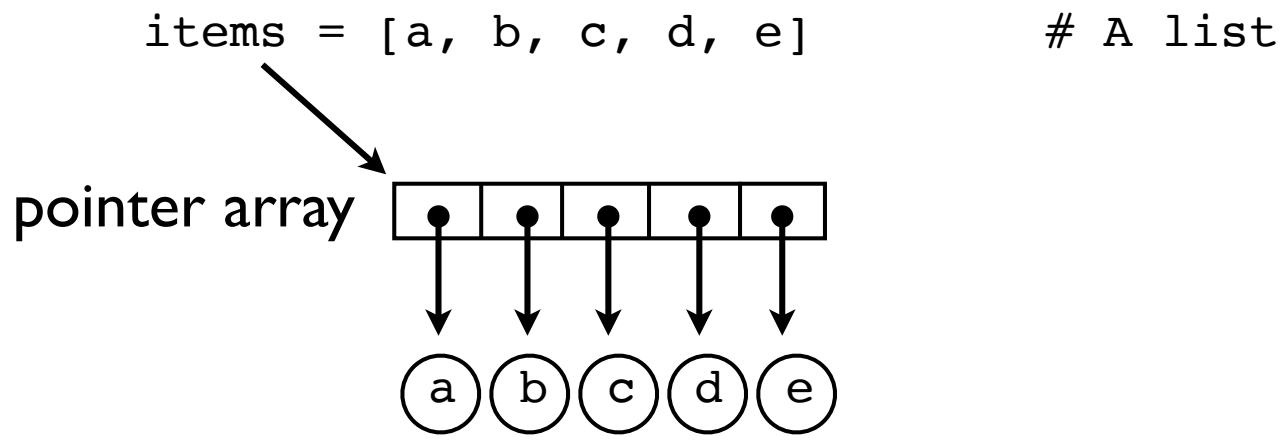
\includegraphics[keepaspectratio]{images/ff7713bd4ddd4348e3cceaf48c2190e01826475c5e16e2a0d0b91d60253c752c.jpg}}

• All operations involving the container internals only manipulate the
pointers (not the objects)

\bookmarksetup{startatroot}

\chapter{Over-allocation}\label{over-allocation}

• All mutable containers (lists, dicts, sets) tend to over-allocate
memory so that there are always some free slots available

\pandocbounded{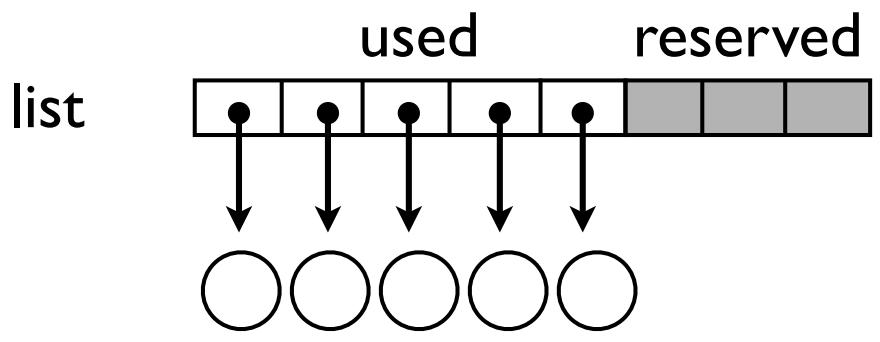
\includegraphics[keepaspectratio]{images/cb0f79d93585d9ef552cc27ffa74e8b15614484d7c6d96332df02392a22a4a49.jpg}}

• This is a performance optimization\\
• Goal is to make appends, insertions fast

\bookmarksetup{startatroot}

\chapter{Example : List Memory}\label{example-list-memory}

• Example of list memory allocation

\begin{Shaded}
\begin{Highlighting}[]
\NormalTok{items = []}
\NormalTok{items.append(1)}
\NormalTok{items.append(2)}
\NormalTok{items.append(3)}
\NormalTok{items.append(4)}
\NormalTok{items.append(5)}
\NormalTok{items.append(6)}
\NormalTok{items.append(7) }
\end{Highlighting}
\end{Shaded}

\pandocbounded{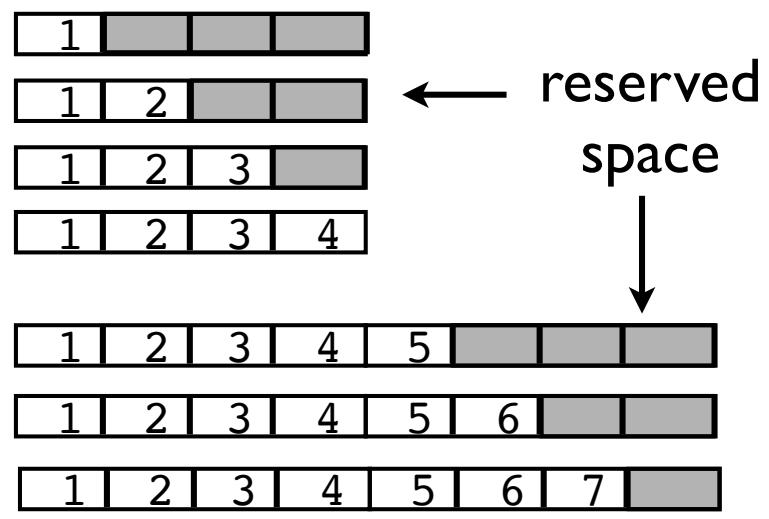
\includegraphics[keepaspectratio]{images/1b1befe6b1b040315580291d02159429c672272d0466226e3d0cda63ad9f1df0.jpg}}

Extra space means that most append() operations are very fast (space is
already available, no memory allocation required)

\bookmarksetup{startatroot}

\chapter{Container Growth}\label{container-growth}

Memory use of containers grows in proportion to the number of stored
values\\
Lists : Increase by \textasciitilde12.5\% when full\\
Sets : Increases by factor 4 when 2/3 full\\
Dicts : Increases by a factor 2 when 2/3 full

\bookmarksetup{startatroot}

\chapter{Set/Dict Hashing}\label{setdict-hashing}

• Sets and dictionaries are based on hashing\\
Keys are used to determine an integer ``hashing value'' (\textbf{hash}()
method)

a = `Python'

b = `Guido'

c = `Dave'

\begin{quote}
\begin{quote}
\begin{quote}
a.\_\_hash\_\_()
\end{quote}
\end{quote}
\end{quote}

-539294296

\begin{quote}
\begin{quote}
\begin{quote}
b.\_\_hash\_\_()
\end{quote}
\end{quote}
\end{quote}

1034194775

\begin{quote}
\begin{quote}
\begin{quote}
c.\_\_hash\_\_()
\end{quote}
\end{quote}
\end{quote}

2135385778

• Value used internally (implementation detail)

\bookmarksetup{startatroot}

\chapter{Key Restrictions}\label{key-restrictions}

• Sets/dict keys restricted to ``hashable'' objects

\begin{Shaded}
\begin{Highlighting}[]
\OperatorTok{\textgreater{}\textgreater{}\textgreater{}} \CharTok{a} \OperatorTok{=} \FunctionTok{\{}\CharTok{\textquotesingle{}IBM\textquotesingle{}}\FunctionTok{,} \CharTok{\textquotesingle{}AA\textquotesingle{}}\FunctionTok{,} \CharTok{\textquotesingle{}AAPL\textquotesingle{}}\FunctionTok{\}}  
\OperatorTok{\textgreater{}\textgreater{}\textgreater{}} \CharTok{b} \OperatorTok{=} \FunctionTok{[[}\DecValTok{1}\FunctionTok{,}\DecValTok{2}\FunctionTok{],} \FunctionTok{[}\DecValTok{3}\FunctionTok{,}\DecValTok{4}\FunctionTok{]]}  
\VariableTok{Traceback} \FunctionTok{(}\CharTok{most} \CharTok{recent} \CharTok{call} \CharTok{last}\FunctionTok{):}  
    \VariableTok{File} \StringTok{"\textless{}stdin\textgreater{}"}\FunctionTok{,} \CharTok{line} \DecValTok{1}\FunctionTok{,} \CharTok{in} \OperatorTok{\textless{}}\CharTok{module}\OperatorTok{\textgreater{}}  
\VariableTok{TypeError}\FunctionTok{:} \CharTok{unhashable} \CharTok{type}\FunctionTok{:} \CharTok{\textquotesingle{}list\textquotesingle{}}  
\OperatorTok{\textgreater{}\textgreater{}\textgreater{}} 
\end{Highlighting}
\end{Shaded}

This usually means you can only use strings, numbers, or tuples (no
lists, dicts, sets, etc.)\\
• Requires \textbf{hash}() and \textbf{eq}() methods

\bookmarksetup{startatroot}

\chapter{Dict Layout}\label{dict-layout}

Hashing in a nutshell\ldots.

\pandocbounded{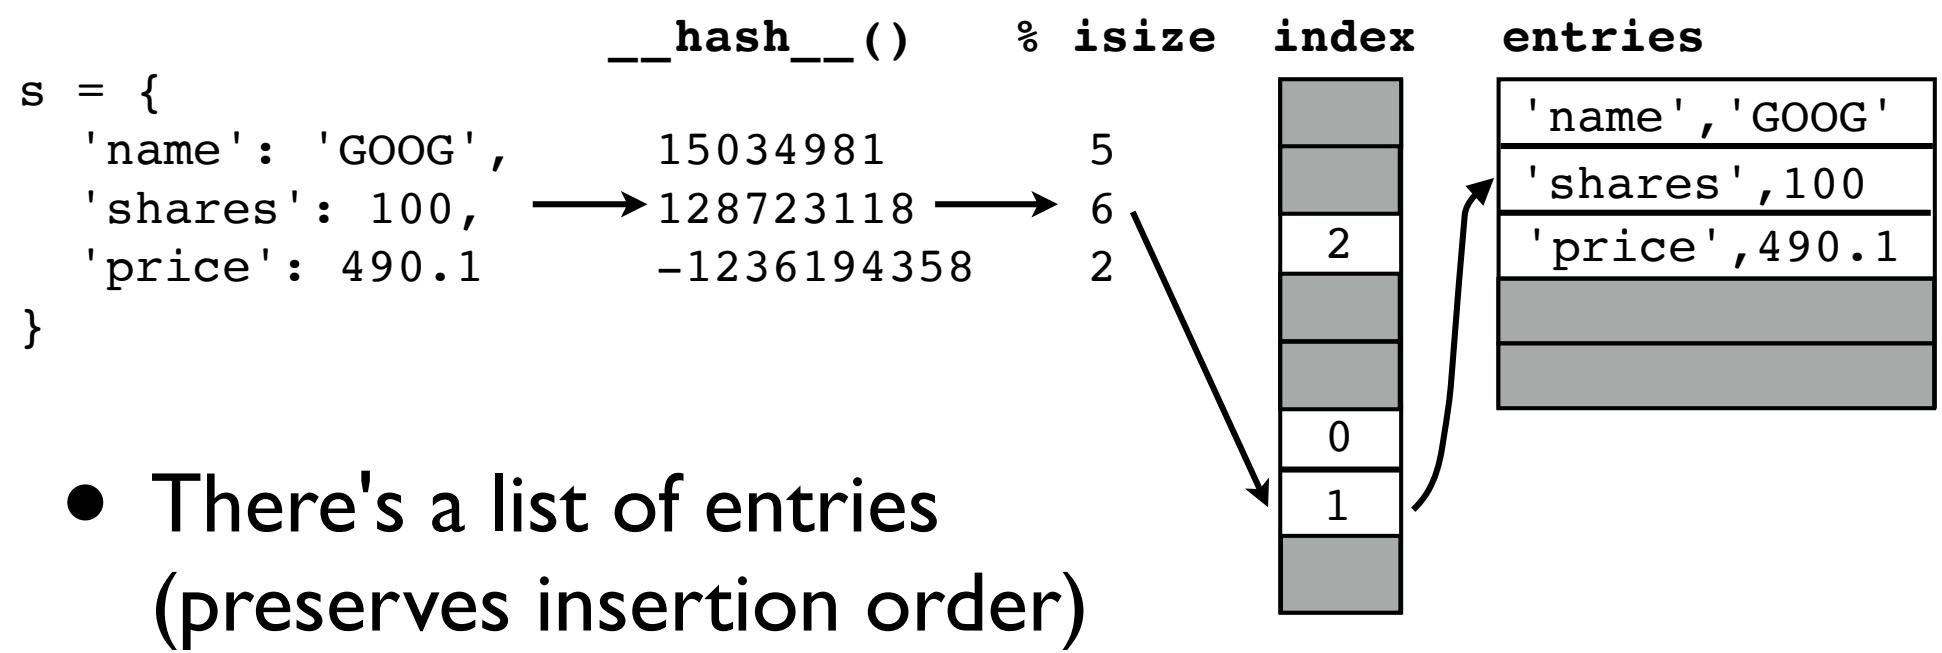
\includegraphics[keepaspectratio]{images/2c3e9c29757e32917c755c9b2d6b35320993ba5eca88ab5f714722333bd4b85c.jpg}}

• A hashed index (holds entry positions)

\bookmarksetup{startatroot}

\chapter{Collision Resolution}\label{collision-resolution}

• Hash index is perturbed until an open slot found

\[
\begin{array}{l} \text {k e y} = ^ {\prime} \text {n a m e} ^ {\prime} \\ h = k e y. \_ \_ h a s h \_ \_ () - > 1 5 0 3 4 9 8 1 \\ i = h \% i s i z e \rightarrow 5 \\ \end{array}
\]

Recurrence

\[
\begin{array}{l} i, h = \text {p e r t u r b} (i, h, \text {s i z e}) \\ i = 7, 6, 1, 4, 5, 2, 3, 0, \dots \\ \end{array}
\]

entry index

\pandocbounded{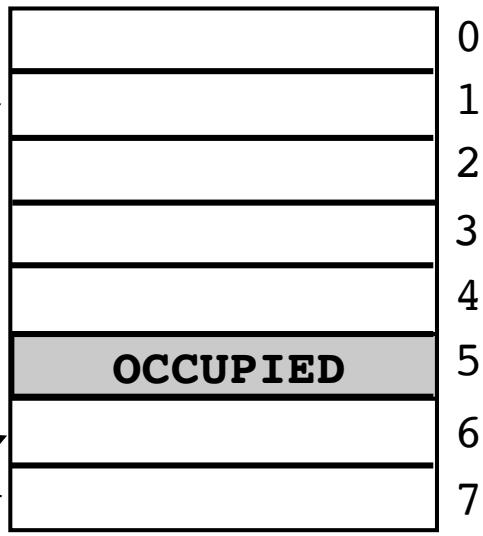
\includegraphics[keepaspectratio]{images/c2b57431a36a669aae282bb55e4e353aa011e4388b15da5eb7b6e6bc265b7ecc.jpg}}

Every slot is tried eventually\\
• Works better if many open slots available

\bookmarksetup{startatroot}

\chapter{Container Protocols}\label{container-protocols}

• Containers also work through ``protocols''

\begin{Shaded}
\begin{Highlighting}[]
\NormalTok{\textgreater{}\textgreater{}\textgreater{} a = [\textquotesingle{}x\textquotesingle{}, \textquotesingle{}y\textquotesingle{}, \textquotesingle{}z\textquotesingle{}]  }
\NormalTok{\textgreater{}\textgreater{}\textgreater{} a[1]  }
\NormalTok{\textquotesingle{}Y\textquotesingle{}  }
\NormalTok{\textgreater{}\textgreater{}\textgreater{} a.\_getitem\_(1) \# Protocol  }
\NormalTok{\textquotesingle{}Y\textquotesingle{}  }
\NormalTok{\textgreater{}\textgreater{}\textgreater{} \textquotesingle{}z\textquotesingle{} in a  }
\NormalTok{True  }
\NormalTok{\textgreater{}\textgreater{}\textgreater{} a.\_contains\_\_( \textquotesingle{}z\textquotesingle{}) \# Protocol  }
\NormalTok{True }
\end{Highlighting}
\end{Shaded}

You can make custom container objects by implementing the required
methods\\
Examples: numpy, Pandas, etc.

\bookmarksetup{startatroot}

\chapter{Container Taxonomy}\label{container-taxonomy}

For new containers, consider collections.abc

Mapping, MutableMapping Sequence, MutableSequence Set, MutableSet

• Use these as a base class

class MyContainer(collections.abc.MutableMapping): .

• Forces you to implement required methods

\begin{Shaded}
\begin{Highlighting}[]
\OperatorTok{\textgreater{}\textgreater{}\textgreater{}}\NormalTok{ c }\OperatorTok{=}\NormalTok{ MyContainer()}
\NormalTok{Traceback (most recent call last):}
\NormalTok{    File }\StringTok{"\textless{}stdin\textgreater{}"}\NormalTok{, line }\DecValTok{1}\NormalTok{, }\KeywordTok{in} \OperatorTok{\textless{}}\NormalTok{module}\OperatorTok{\textgreater{}}
\PreprocessorTok{TypeError}\NormalTok{: Can}\StringTok{\textquotesingle{}t instantiate abstract class MyContainer with abstract methods \_\_delitem\_\_, \_\_getitem\_\_, \_\_iter\_\_, \_\_len\_\_, \_\_setitem\_\_}
\ErrorTok{\textgreater{}\textgreater{}\textgreater{} }
\end{Highlighting}
\end{Shaded}

\bookmarksetup{startatroot}

\chapter{Exercise 2.5}\label{exercise-2.5}

Time : 25 Minutes

\bookmarksetup{startatroot}

\chapter{Understanding Assignment}\label{understanding-assignment}

Many operations in Python are related to ``assigning'' or ``storing''
values

a = value \# Assignment to a variable

s{[}n{]} = value \# Assignment to an list

s.append(value) \# Appending to a list

d{[}`key'{]} = value \# Adding to a dictionary

• A caution : assignment operations never make a copy of the value being
assigned\\
• All assignments are merely reference copies (or pointer copies if you
prefer)

\bookmarksetup{startatroot}

\chapter{Assignment Example}\label{assignment-example}

• Consider this code fragment:

\[
\begin{array}{l} a = [ 1, 2, 3 ] \\ b = a \\ c = [ a, b ] \\ \end{array}
\]

• A picture of the underlying memory

\pandocbounded{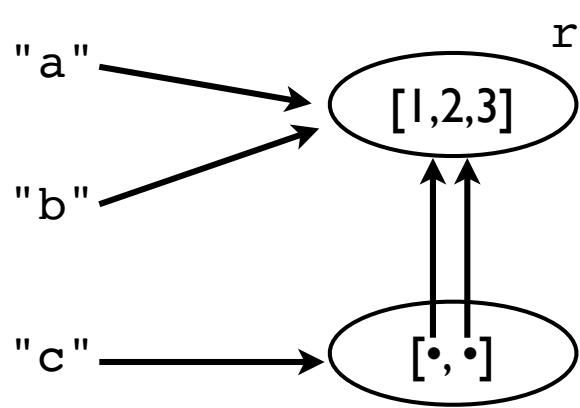
\includegraphics[keepaspectratio]{images/c3e06085d79345ab52e10a2543072fd22601262056931e8d32e546cb76f70820.jpg}}

\[
\mathrm {r e f} = 4
\]

There is only one list object {[}1,2,3{]}, but there are four different
references to it.

\bookmarksetup{startatroot}

\chapter{Assignment Caution}\label{assignment-caution}

Modifying a value affects all references

\begin{Shaded}
\begin{Highlighting}[]
\VariableTok{\textgreater{}\textgreater{}\textgreater{} a.append(999)  }
\VariableTok{\textgreater{}\textgreater{}\textgreater{} a  }
\NormalTok{[1,2,3,999]  }
\VariableTok{\textgreater{}\textgreater{}\textgreater{} b  }
\NormalTok{[1,2,3,999]  }
\VariableTok{\textgreater{}\textgreater{}\textgreater{} c  }
\NormalTok{[[1,2,3,999], [1,2,3,999]]  }
\VariableTok{\textgreater{}\textgreater{}\textgreater{} }
\end{Highlighting}
\end{Shaded}

• Notice how a change to the original list shows up everywhere else
(yikes!)\\
This is because no copies were ever made-- everything is pointing at the
same thing

\bookmarksetup{startatroot}

\chapter{Call by Object}\label{call-by-object}

• Objects are never copied on function call

def func(items): items.append(42)

\begin{Shaded}
\begin{Highlighting}[]
\NormalTok{\textgreater{}\textgreater{}\textgreater{} a = [1,2,3]  }
\NormalTok{\textgreater{}\textgreater{}\textgreater{} func(a)  }
\NormalTok{\textgreater{}\textgreater{}\textgreater{} a  }
\NormalTok{[1, 2, 3, 42]  }
\NormalTok{\textgreater{}\textgreater{}\textgreater{} }
\end{Highlighting}
\end{Shaded}

• Mutations affect the original object\\
Reminder: many objects are immutable

\bookmarksetup{startatroot}

\chapter{Reassigning Names}\label{reassigning-names}

• Reassigning a name never overwrites the memory used by the previous
value

\[
\begin{array}{l} a = [ 1, 2, 3 ] \\ \texttt {b} = \texttt {a} \\ \end{array}
\]

\pandocbounded{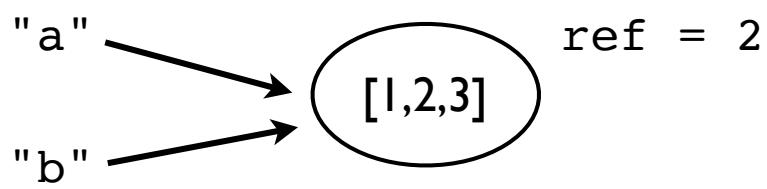
\includegraphics[keepaspectratio]{images/9af277c35fb7b7553d3db5c0dcbc3872cc873d4f045f26f1b69ef82495c22b0a.jpg}}

\[
a = [ 4, 5, 6 ]
\]

\pandocbounded{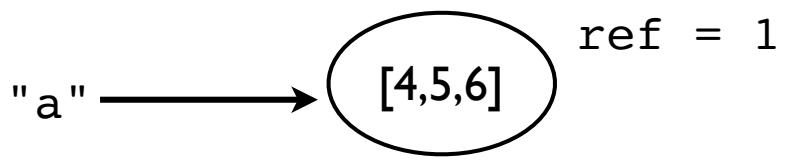
\includegraphics[keepaspectratio]{images/9f6232538264fcdf0fb7f8f9ea98db4df207c64327dedd9270d686713b4eacea.jpg}}

\pandocbounded{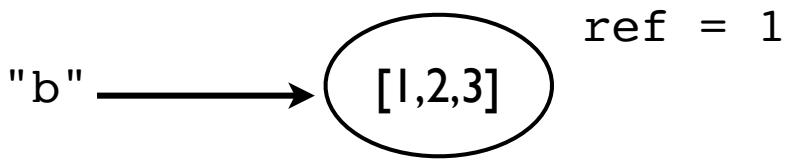
\includegraphics[keepaspectratio]{images/63d8fb0fab2ac72f0138d03c528f46f91c4a7f78cb7e2506bb92ee20f5ffef94.jpg}}

• The name now refers to a different object

\bookmarksetup{startatroot}

\chapter{Identity and References}\label{identity-and-references}

• Use the ``is'' operator to check if two values are exactly the same in
memory

\[
\begin{array}{l} \ggg a = [ 1, 2, 3 ] \\ \ggg \mathbf {b} = \mathbf {a} \\ \ggg a i s b \\ \mathbf {T r u e} \\ \ggg \\ \end{array}
\]

• Every object also has an integer identifier

\[
\begin{array}{l} \ggg \mathbf {i d} (\mathbf {a}) \\ 2 7 7 4 7 6 0 \\ \ggg \mathbf {i d} (\mathbf {b}) \\ 2 7 7 4 7 6 0 \\ \ggg \\ \end{array}
\]

The object identifier is kind of like

a pointer. If two names have the

same id value, they're referring to

the same object.

\bookmarksetup{startatroot}

\chapter{Exploiting Immutability}\label{exploiting-immutability}

Immutable values can be safely shared

\pandocbounded{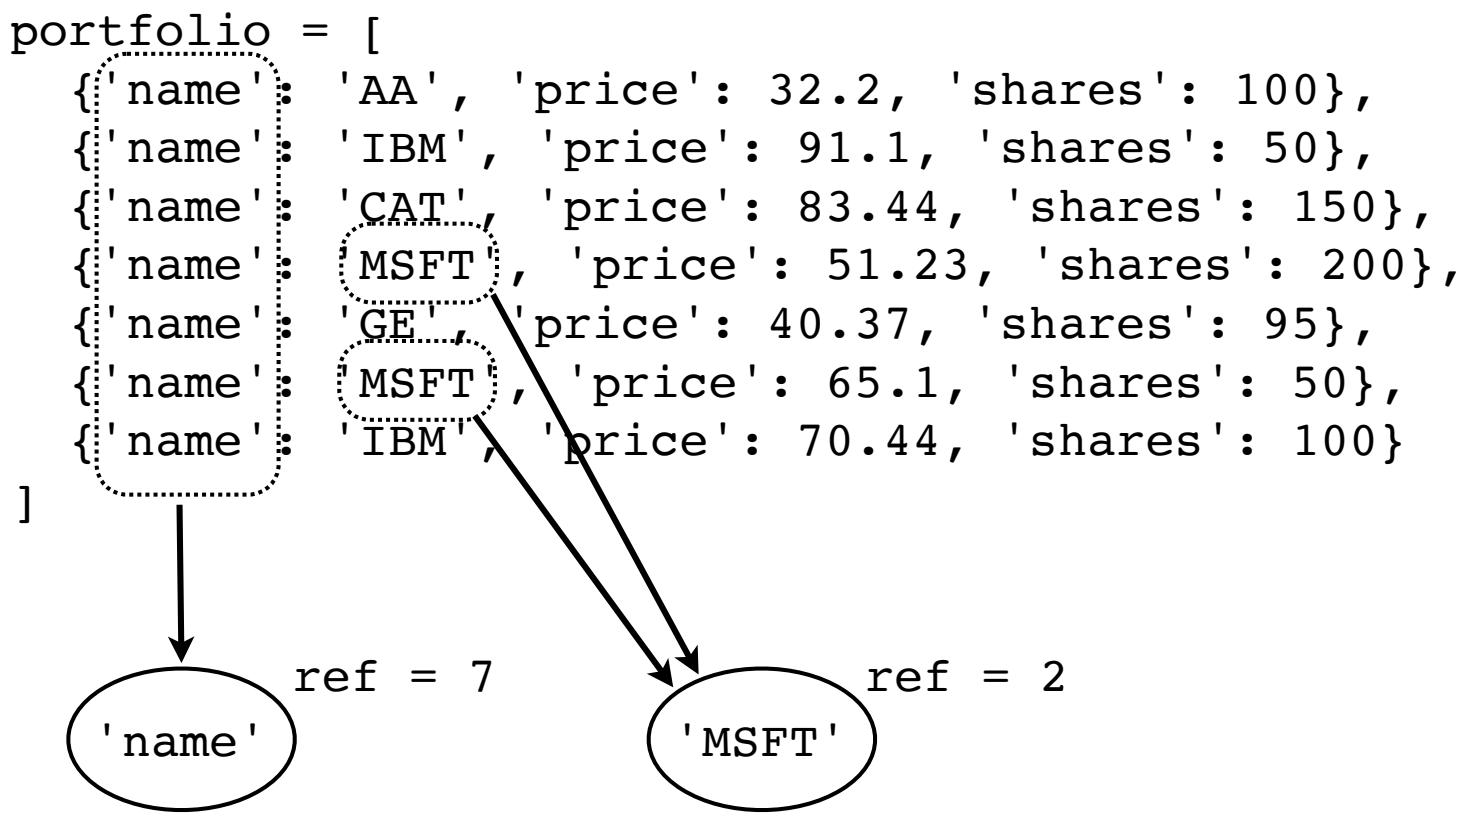
\includegraphics[keepaspectratio]{images/d8933cd1056db76a1d3361beb63acee84c6055f8134d03e851837aa53f663372.jpg}}

• Sharing can save significant memory

\bookmarksetup{startatroot}

\chapter{Shallow Copies}\label{shallow-copies}

• Containers have methods for copying

\[
\begin{array}{l} \ggg a = [ 2, 3, [ 1 0 0, 1 0 1 ], 4 ] \\ \ggg \mathbf {b} = \operatorname {l i s t} (\mathbf {a}) \\ \ggg a i s b \\ \end{array}
\]

False

\bookmarksetup{startatroot}

\chapter{Make a copy}\label{make-a-copy}

• However, items are copied by reference

\[
\begin{array}{l} \ggg a [ 2 ] \cdot a p p e n d (1 0 2) \\ \ggg \mathbf {b} [ 2 ] \\ [ 1 0 0, 1 0 1, 1 0 2 ] \\ \ggg \\ \end{array}
\]

This inner list is still being shared

\pandocbounded{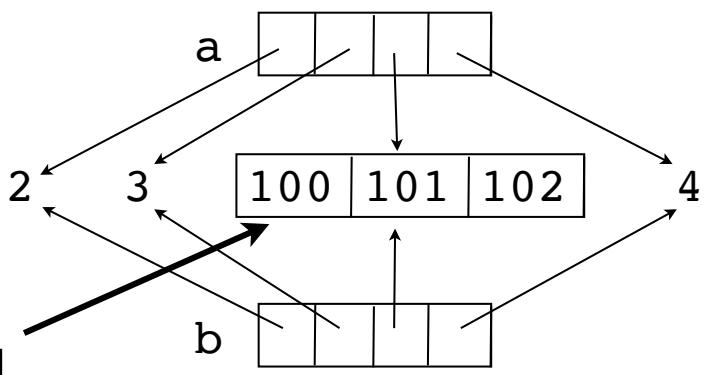
\includegraphics[keepaspectratio]{images/914c2931efd4a0810dabd580979349d97ede2741bb87b9a9d974e2ed9c55c973.jpg}}

Known as a ``shallow copy''

\bookmarksetup{startatroot}

\chapter{Deep Copying}\label{deep-copying}

Sometimes you need to makes a copy of an object and all objects
contained within it\\
Use the copy module

\begin{Shaded}
\begin{Highlighting}[]
\NormalTok{\textgreater{}\textgreater{}\textgreater{} a = [2,3,[100,101],4]  }
\NormalTok{\textgreater{}\textgreater{}\textgreater{} import copy  }
\NormalTok{\textgreater{}\textgreater{}\textgreater{} b = copy.copy(a)  }
\NormalTok{\textgreater{}\textgreater{}\textgreater{} a[2].append(102)  }
\NormalTok{\textgreater{}\textgreater{}\textgreater{} b[2]  }
\NormalTok{[100,101]  }
\NormalTok{\textgreater{}\textgreater{}\textgreater{} }
\end{Highlighting}
\end{Shaded}

• This is the only safe way to copy something

\bookmarksetup{startatroot}

\chapter{Everything is an object}\label{everything-is-an-object}

• Numbers, strings, lists, functions, exceptions, classes, instances,
etc\ldots{}\\
• All objects are said to be ``first-class''\\
Meaning: All objects that can be named can be passed around as data,
placed in containers, etc., without any restrictions.\\
• There are no ``special'' kinds of objects

\bookmarksetup{startatroot}

\chapter{Example: Emulating Cases}\label{example-emulating-cases}

A big conditional with many cases

Reformulation using a dict of functions

if op \(= =\) ' +`:\\
r = add(x, y)\\
elif op =='-`:\\
r = sub(x, y)\\
elif op =='*`:\\
r = mul(x, y)\\
elif op =='/':\\
r = div(x, y)

\pandocbounded{
\includegraphics[keepaspectratio]{images/34bc51d7938af88870afecbce0660ae393e0bbfbf6c3061c30edd1436b48194d.jpg}}

ops \(=\) \{
\(\begin{array}{rl}{\mathrm{\bf~\sf~\sf~\sf~\sf~\sf~\sf~\sf~\sf~\sf~\sf~\sf~\sf~\sf~\sf~\sf~\sf~\sf~\sf~\sf~\sf~\sf~\sf~\sf~\sf~\sf~\sf~\sf~\sf~\sf~\sf~\sf~\sf~\sf~\sf ~}} & {}\\ {\mathrm{\bf~\sf~\sf~\sf~\sf~\sf~\sf~\sf~\sf~\sf~\sf~\sf~\sf~\sf~\sf~\sf~\sf~\sf~\sf~\sf~\sf~\sf~\sf~\sf~\sf~\sf~\sf~\sf~\sf~\sf~\sf~\sf~\sf ~}} & {{}^{\prime} + {}^{\prime}\quad :  \mathrm{add},}\\ {\mathrm{\bf~\sf~\sf~\sf~\sf~\sf~\sf~\sf~\sf~\sf~\sf~\sf~\sf~\sf~\sf~\sf~\sf~\sf~\sf~\sf~\sf~\sf~\sf~\sf~\sf~ \mathrm{sub}},}\\ {\mathrm{\bf~\sf~\sf~\sf~\sf~\sf~\sf~\sf~\sf~\sf~\sf~\sf~ \mathrm{mul}},}\\ {\mathrm{\bf~\sf~ \mathrm{ / / } \mathrm{ : ~ \rm div}}} \\ \end{array}\)
\}\\
r \(=\) ops\href{x,y}{op}

• Key idea: Can make data structures from anything

\bookmarksetup{startatroot}

\chapter{Exercise 2.6}\label{exercise-2.6}

Time : 25 Minutes

\bookmarksetup{startatroot}

\chapter{Section 3}\label{section-3}

\bookmarksetup{startatroot}

\chapter{Classes and Objects}\label{classes-and-objects}

\bookmarksetup{startatroot}

\chapter{When to use Objects?}\label{when-to-use-objects}

Object oriented programming is largely concerned with the modeling of
``behavior.''\\
• An ``object'' consists of some internal state, but more importantly,
has methods that make it do various things.\\
• The methods give an object its personality

\bookmarksetup{startatroot}

\chapter{An Example}\label{an-example}

Data

\[
\text {h o s t} = \left(^ {\prime} \mathrm {w w w}. \text {p y t h o n}. \mathrm {o r g} ^ {\prime}, 8 0\right)
\]

Behavior

\begin{Shaded}
\begin{Highlighting}[]
\NormalTok{c = Connection(\textquotesingle{}www.python.org\textquotesingle{}, 80)  }
\NormalTok{c.open()  }
\NormalTok{c.send(data)  }
\NormalTok{c.recv()  }
\NormalTok{c.close() }
\end{Highlighting}
\end{Shaded}

Data and behavior are bound together

\bookmarksetup{startatroot}

\chapter{The class statement}\label{the-class-statement}

• Use `class' to define a new object

class Player:

\begin{Shaded}
\begin{Highlighting}[]
\KeywordTok{def} \FunctionTok{\_\_init\_\_}\NormalTok{(}\VariableTok{self}\NormalTok{, x, y):}
    \VariableTok{self}\NormalTok{.x }\OperatorTok{=}\NormalTok{ x}
    \VariableTok{self}\NormalTok{.y }\OperatorTok{=}\NormalTok{ y}
    \VariableTok{self}\NormalTok{.health }\OperatorTok{=} \DecValTok{100} 
\end{Highlighting}
\end{Shaded}

\begin{Shaded}
\begin{Highlighting}[]
\KeywordTok{def}\NormalTok{ move(}\VariableTok{self}\NormalTok{, dx, dy):}
    \VariableTok{self}\NormalTok{.dx }\OperatorTok{+=}\NormalTok{ dx}
    \VariableTok{self}\NormalTok{.dy }\OperatorTok{+=}\NormalTok{ dy }
\end{Highlighting}
\end{Shaded}

def damage(self, pts): self.health \(= =\) pts

• What is a class?\\
Mostly, it's a set of functions that carry out various operations on
so-called ``instances''

\bookmarksetup{startatroot}

\chapter{Instances}\label{instances-1}

Instances are the actual ``objects'' that you manipulate in your
program\\
• Created by calling the class as a function

\begin{quote}
\begin{quote}
\begin{quote}
a = Player(2, 3)\\
b = Player(10, 20)
\end{quote}
\end{quote}
\end{quote}

Emphasize: The class statement is just the definition (it does nothing
by itself)

\bookmarksetup{startatroot}

\chapter{Instance Data}\label{instance-data}

• Each instance has its own local data

\begin{Shaded}
\begin{Highlighting}[]
\NormalTok{\textgreater{}\textgreater{}\textgreater{} a.x 2   }
\NormalTok{\textgreater{}\textgreater{}\textgreater{} b.x 10 }
\end{Highlighting}
\end{Shaded}

• This data is initialized by \textbf{init}()

\begin{Shaded}
\begin{Highlighting}[]
\KeywordTok{class}\NormalTok{ Player: }\KeywordTok{def} \FunctionTok{\_\_init\_\_}\NormalTok{(}\VariableTok{self}\NormalTok{, x, y):  }
    \VariableTok{self}\NormalTok{.x }\OperatorTok{=}\NormalTok{ x  }
    \VariableTok{self}\NormalTok{.y }\OperatorTok{=}\NormalTok{ y  }
    \VariableTok{self}\NormalTok{.health }\OperatorTok{=} \DecValTok{100}  
\KeywordTok{is}\NormalTok{ instance data }
\end{Highlighting}
\end{Shaded}

• There are no restrictions on the total number or type of attributes
stored

\bookmarksetup{startatroot}

\chapter{Instance Methods}\label{instance-methods}

Functions applied to instances of an object class Player:

\begin{Shaded}
\begin{Highlighting}[]
\KeywordTok{def}\NormalTok{ move(}\VariableTok{self}\NormalTok{, dx, dy): }\VariableTok{self}\NormalTok{.x }\OperatorTok{+=}\NormalTok{ dx }\VariableTok{self}\NormalTok{.y }\OperatorTok{+=}\NormalTok{ dy }
\end{Highlighting}
\end{Shaded}

• The object is always passed as first argument

\begin{Shaded}
\begin{Highlighting}[]
\NormalTok{\textgreater{}\textgreater{}\textgreater{} a.move(1, 2) def move(self, dx, dy): ... }
\end{Highlighting}
\end{Shaded}

By convention, the instance is called ``self''

The name is unimportant---the object is always passed as the first
argument. It is simply Python programming style to call this argument
``self.''

\bookmarksetup{startatroot}

\chapter{Attributes}\label{attributes}

• A word on terminology\\
``Attribute'' is anything accessed via (.)

\begin{quote}
\begin{quote}
\begin{quote}
a.x \# Attribute of an instance 2\\
Player.move \# Attribute of a class \textless function Player.move at
0x10e7f6400\textgreater{}\\
import math\\
math.pi \# Attribute of a module
\end{quote}
\end{quote}
\end{quote}

Don't read too much into it

\bookmarksetup{startatroot}

\chapter{History Lesson}\label{history-lesson}

Python classes were one of the last major features implemented in the
language\\
Design goals included no changes in syntax (other than the class
statement itself) and no changes to function scoping rules\\
Hence : Instance methods are normal function definitions that simply
receive the instance as the first argument (self)\\
That's it

\bookmarksetup{startatroot}

\chapter{Class Scoping}\label{class-scoping}

Caution: Classes do not define a scope

\begin{Shaded}
\begin{Highlighting}[]
\OperatorTok{\textgreater{}\textgreater{}\textgreater{}} \PreprocessorTok{NameError}
\KeywordTok{class}\NormalTok{ Player:}
\NormalTok{    ...}
    \KeywordTok{def}\NormalTok{ move(}\VariableTok{self}\NormalTok{, dx, dy):}
        \VariableTok{self}\NormalTok{.x }\OperatorTok{+=}\NormalTok{ dx}
        \VariableTok{self}\NormalTok{.y }\OperatorTok{+=}\NormalTok{ dy}
    \KeywordTok{def}\NormalTok{ left(}\VariableTok{self}\NormalTok{, amt):}
\NormalTok{        move(}\OperatorTok{{-}}\NormalTok{amt, }\DecValTok{0}\NormalTok{)  }\CommentTok{\# NO. Calls global move()}
        \VariableTok{self}\NormalTok{.move(}\OperatorTok{{-}}\NormalTok{amt, }\DecValTok{0}\NormalTok{)  }\CommentTok{\# YES. }
\end{Highlighting}
\end{Shaded}

If want to operate on an instance, you always have to refer to it
explicitly (e.g., self)

\bookmarksetup{startatroot}

\chapter{Exercise 3.1}\label{exercise-3.1}

Time : 20 Minutes

\bookmarksetup{startatroot}

\chapter{Manipulating Instances}\label{manipulating-instances}

• There are only three operations on instances

obj Attr \#Get an attribute obj.Attr \(=\) value \#Set an attribute del
obj.Attr \#Delete an attribute

Attributes can be freely added and deleted after an instance is created

\begin{Shaded}
\begin{Highlighting}[]
\NormalTok{\textgreater{}\textgreater{}\textgreater{} s = Stock(\textquotesingle{}ACME\textquotesingle{}, 50, 91.1)  }
\NormalTok{\textgreater{}\textgreater{}\textgreater{} s.share  }
\NormalTok{50  }
\NormalTok{\textgreater{}\textgreater{}\textgreater{} s.date = \textquotesingle{}10/31/2017\textquotesingle{} \# Add an attribute  }
\NormalTok{\textgreater{}\textgreater{}\textgreater{} del s.name \# Delete an attribute  }
\NormalTok{\textgreater{}\textgreater{}\textgreater{} }
\end{Highlighting}
\end{Shaded}

\bookmarksetup{startatroot}

\chapter{Attribute Access Functions}\label{attribute-access-functions}

These functions may be used to manipulate attributes given an attribute
name string

\begin{Shaded}
\begin{Highlighting}[]
\BuiltInTok{getattr}\NormalTok{(obj, }\StringTok{\textquotesingle{}name\textquotesingle{}}\NormalTok{) }\CommentTok{\# Same as obj.name  }
\BuiltInTok{setattr}\NormalTok{(obj, }\StringTok{\textquotesingle{}name\textquotesingle{}}\NormalTok{, value) }\CommentTok{\# Same as obj.name = value  }
\BuiltInTok{delattr}\NormalTok{(obj, }\StringTok{\textquotesingle{}name\textquotesingle{}}\NormalTok{) }\CommentTok{\# Same as del obj.name  }
\BuiltInTok{hasattr}\NormalTok{(obj, }\StringTok{\textquotesingle{}name\textquotesingle{}}\NormalTok{) }\CommentTok{\# Tests if attribute exists }
\end{Highlighting}
\end{Shaded}

Example: Output

\begin{Shaded}
\begin{Highlighting}[]
\NormalTok{attributes }\OperatorTok{=}\NormalTok{ [}\StringTok{\textquotesingle{}name\textquotesingle{}}\NormalTok{, }\StringTok{\textquotesingle{}shares\textquotesingle{}}\NormalTok{, }\StringTok{\textquotesingle{}price\textquotesingle{}}\NormalTok{]}
\ControlFlowTok{for}\NormalTok{ attr }\KeywordTok{in}\NormalTok{ attributes:}
    \BuiltInTok{print}\NormalTok{(attr, }\StringTok{\textquotesingle{}:=\textquotesingle{}}\NormalTok{ , }\BuiltInTok{getattr}\NormalTok{(obj, attr)) }
\end{Highlighting}
\end{Shaded}

• Note: getattr() has a useful default value arg

\begin{Shaded}
\begin{Highlighting}[]
\NormalTok{x = getattr(obj, \textquotesingle{}x\textquotesingle{}, None) }
\end{Highlighting}
\end{Shaded}

\bookmarksetup{startatroot}

\chapter{Method Invocation}\label{method-invocation}

• Invoking a method is a two-step process\\
Lookup: The . operator\\
• Method call: The () operator

class Stock: def cost(self): return self.share * self.price
\textgreater\textgreater\textgreater s =Stock(`ACME'，50,91.1)
\textgreater\textgreater\textgreater c \(=\) s.cost Lookup
\textgreater\textgreater\textgreater c \textless bound method Stock.cost
of \textless Stock object at 0x590d0\textgreater\textgreater{}
\textgreater\textgreater\textgreater{} c() 4555.0 Method call

\bookmarksetup{startatroot}

\chapter{Bound Methods}\label{bound-methods}

A method that has not yet been invoked by the function call operator ()
is known as a ``bound method''\\
• It operates on the instance where it originated

\begin{quote}
\begin{quote}
\begin{quote}
s = Stock(`ACME'，50,91.1)\\
s\\
STOCKobjectat \(0\mathrm{x}590\mathrm{d}0>\)
\textgreater\textgreater\textgreater c \(\equiv\) s.cost binding\\
c\\
\textless bound methodStock.cost of \textless Stock object at
0x590d0\textgreater\textgreater{}\\
c()\\
4555.0
\end{quote}
\end{quote}
\end{quote}

\bookmarksetup{startatroot}

\chapter{Bound Methods}\label{bound-methods-1}

Why would you care?\\
• Often a source of careless non-obvious errors

\begin{Shaded}
\begin{Highlighting}[]
\NormalTok{\textgreater{}\textgreater{}\textgreater{} s = Stock(\textquotesingle{}ACME\textquotesingle{}, 50, 91.1)  }
\NormalTok{\textgreater{}\textgreater{}\textgreater{} print(\textquotesingle{}Cost: \%0.2f\textquotesingle{} \% s.cost)  }
\NormalTok{Traceback (most recent call last):  }
\NormalTok{    File "\textless{}stdin\textgreater{}", line 1, in \textless{}module\textgreater{}  }
\NormalTok{TypeError: a float is required  }
\NormalTok{\textgreater{}\textgreater{}\textgreater{} }
\end{Highlighting}
\end{Shaded}

• Or devious behavior that's hard to debug

f = open(filename, `w')\\
\ldots{}\\
f.close \(\leftarrow\) Oops. Didn't do anything at all

\bookmarksetup{startatroot}

\chapter{Exercise 3.2}\label{exercise-3.2}

Time : 15 Minutes

\bookmarksetup{startatroot}

\chapter{More on Class Definitions}\label{more-on-class-definitions}

• A class contains definitions that are shared by all instances of the
class

\begin{Shaded}
\begin{Highlighting}[]
\KeywordTok{class}\NormalTok{ Stock: }\KeywordTok{def} \FunctionTok{\_\_init\_\_}\NormalTok{(}\VariableTok{self}\NormalTok{, name, shares, price): }\VariableTok{self}\NormalTok{.name }\OperatorTok{=}\NormalTok{ name }\VariableTok{self}\NormalTok{.share }\OperatorTok{=}\NormalTok{ shares }\VariableTok{self}\NormalTok{.price }\OperatorTok{=}\NormalTok{ price }
\end{Highlighting}
\end{Shaded}

\begin{Shaded}
\begin{Highlighting}[]
\KeywordTok{def}\NormalTok{ cost(}\VariableTok{self}\NormalTok{):}
    \ControlFlowTok{return} \VariableTok{self}\NormalTok{.share }\OperatorTok{*} \VariableTok{self}\NormalTok{.price }
\end{Highlighting}
\end{Shaded}

• Shared : Defined once, used by all instances\\
Example : There is one cost() function that gets used by all instances
created

\bookmarksetup{startatroot}

\chapter{Class Variables}\label{class-variables}

Classes may also define variables\\
• Known as ``class variables''

class SomeClass: debug \(=\) False def init\_self, x): self.x = x

• There are two access routes

\begin{Shaded}
\begin{Highlighting}[]
\NormalTok{\textgreater{}\textgreater{}\textgreater{} SomeClass(debug  }
\NormalTok{False  }
\NormalTok{\textgreater{}\textgreater{}\textgreater{} s = SomeClass(42)  }
\NormalTok{\textgreater{}\textgreater{}\textgreater{} s(debug  }
\NormalTok{False  }
\NormalTok{\textgreater{}\textgreater{}\textgreater{} }
\end{Highlighting}
\end{Shaded}

\begin{Shaded}
\begin{Highlighting}[]
\NormalTok{(On the class itself) (On an instance of the class) }
\end{Highlighting}
\end{Shaded}

\bookmarksetup{startatroot}

\chapter{Using Class Variables}\label{using-class-variables}

• Often used for settings applied to all instances

\begin{Shaded}
\begin{Highlighting}[]
\KeywordTok{class}\NormalTok{ Date: datefmt }\OperatorTok{=} \StringTok{\textquotesingle{}}\SpecialCharTok{\{year\}}\StringTok{{-}}\SpecialCharTok{\{month\}}\StringTok{{-}}\SpecialCharTok{\{day\}}\StringTok{\textquotesingle{}} \KeywordTok{def} \FunctionTok{\_\_init\_\_}\NormalTok{(}\VariableTok{self}\NormalTok{, year, month, day): }\VariableTok{self}\NormalTok{.year }\OperatorTok{=}\NormalTok{ year }\VariableTok{self}\NormalTok{.month }\OperatorTok{=}\NormalTok{ month }\VariableTok{self}\NormalTok{.day }\OperatorTok{=}\NormalTok{ day }\KeywordTok{def} \FunctionTok{\_\_str\_\_}\NormalTok{(}\VariableTok{self}\NormalTok{): }\ControlFlowTok{return} \VariableTok{self}\NormalTok{.datefmt.}\BuiltInTok{format}\NormalTok{(year}\OperatorTok{=} \VariableTok{self}\NormalTok{.year, month}\OperatorTok{=} \VariableTok{self}\NormalTok{.month, day}\OperatorTok{=} \VariableTok{self}\NormalTok{.day) }
\end{Highlighting}
\end{Shaded}

Possibly changed via inheritance

\begin{Shaded}
\begin{Highlighting}[]
\KeywordTok{class}\NormalTok{ USDate(Date):}
\NormalTok{    datefmt }\OperatorTok{=} \StringTok{\textquotesingle{}}\SpecialCharTok{\{month\}}\StringTok{\textquotesingle{}}\OperatorTok{/}\NormalTok{\{day\}}\StringTok{\textquotesingle{}/}\SpecialCharTok{\{year\}}\StringTok{\textquotesingle{}} 
\end{Highlighting}
\end{Shaded}

\bookmarksetup{startatroot}

\chapter{Class Methods}\label{class-methods}

• A method that operates on the class itself

\begin{Shaded}
\begin{Highlighting}[]
\NormalTok{class SomeClass: @classmethod def yow(cls): print(\textquotesingle{}SomeClass.yow\textquotesingle{},cls) }
\end{Highlighting}
\end{Shaded}

• It's invoked on the class, not an instance

\begin{Shaded}
\begin{Highlighting}[]
\NormalTok{\textgreater{}\textgreater{}\textgreater{} SomeClass.yow()}
\NormalTok{SomeClass.yow \textless{}class \_\_main\_\_.SomeClass\textgreater{}}
\NormalTok{\textgreater{}\textgreater{}\textgreater{} }
\end{Highlighting}
\end{Shaded}

• The class is passed as the first argument

\begin{Shaded}
\begin{Highlighting}[]
\NormalTok{SomeClass.yow() @classmethod def yow(c1s): }
\end{Highlighting}
\end{Shaded}

\bookmarksetup{startatroot}

\chapter{Using Class Methods}\label{using-class-methods}

Class methods are often used as a tool for defining alternate
initializers

class Date: def \textbf{init}(self, year, month, day): self.year \(=\)
year self.month \(=\) month self.day \(\equiv\) day
(\textbf{classsmethod?}) def today(c1s): tm \(=\) time.localtime()
return c1s(tm.tm\_year, tm.tm\_mon, tm.tm\_mday) Notice how the class
passed as an argument. d \(=\) Date.Today()

\bookmarksetup{startatroot}

\chapter{Using Class Methods}\label{using-class-methods-1}

• Class methods solve some tricky problems with features like
inheritance

class Date:\\
\ldots{}\\
(\textbf{classmethod?})\\
def today(c1s): tm \(=\) time.localtime() return c1s(tm.tm\_year,
tm.tm\_mon, tm.tm\_mday)\\
class NewDate(Date): Gets the correct class (e.g.,NewDate)\\
d \(=\) NewDate.Today()

\bookmarksetup{startatroot}

\chapter{Static Methods}\label{static-methods}

• A function that's defined as part of a class, but does not operate on
instances or the class

\begin{Shaded}
\begin{Highlighting}[]
\ControlFlowTok{class} \WarningTok{SomeClass:} \OtherTok{@staticmethod} \ControlFlowTok{def}\NormalTok{ yow()}\OperatorTok{:} \FunctionTok{print}\NormalTok{(}\VerbatimStringTok{\textquotesingle{}SomeClass.yow\textquotesingle{}}\NormalTok{) }
\end{Highlighting}
\end{Shaded}

• Example:

\begin{Shaded}
\begin{Highlighting}[]
\NormalTok{\textgreater{}\textgreater{}\textgreater{} SomeClass.yow()  }
\NormalTok{SomeClass.yow  }
\NormalTok{\textgreater{}\textgreater{}\textgreater{} }
\end{Highlighting}
\end{Shaded}

• Notice: There is no hidden self argument

\bookmarksetup{startatroot}

\chapter{Using Static Methods}\label{using-static-methods}

Uses vary:

• Utility functions used by various methods\\
Instance management/tracking\\
• Finalization, resource management\\
Certain design patterns

Might improve code clarity--grouping related functionality together
within a class

\bookmarksetup{startatroot}

\chapter{Exercise 3.3}\label{exercise-3.3}

Time : 15 Minutes

\bookmarksetup{startatroot}

\chapter{Classes and Encapsulation}\label{classes-and-encapsulation}

One of the primary roles of a class is to encapsulate data and internal
implementation details of an object\\
However, a class also defines a ``public'' interface that the outside
world is supposed to use to manipulate the object\\
This distinction between implementation details and the public interface
is important

\bookmarksetup{startatroot}

\chapter{Python Encapsulation}\label{python-encapsulation}

Python relies on programming conventions to indicate the intended use of
something\\
Typically, this is based on naming\\
There is a general attitude that it is up to the programmer to observe
the rules as opposed to having the language enforce rules

\bookmarksetup{startatroot}

\chapter{Private Attributes}\label{private-attributes}

Any attribute name with a leading \_ is considered to be ``private''

\begin{Shaded}
\begin{Highlighting}[]
\KeywordTok{class}\NormalTok{ Base: }\KeywordTok{def} \FunctionTok{\_\_init\_\_}\NormalTok{(}\VariableTok{self}\NormalTok{, name): }\VariableTok{self}\NormalTok{.\_name }\OperatorTok{=}\NormalTok{ name }
\end{Highlighting}
\end{Shaded}

• However, this is only a programming style\\
You can still access it

\begin{Shaded}
\begin{Highlighting}[]
\NormalTok{\textgreater{}\textgreater{}\textgreater{} b = Base(\textquotesingle{}Guido\textquotesingle{})}
\NormalTok{\textgreater{}\textgreater{}\textgreater{} b.\_name}
\NormalTok{\textquotesingle{}Guido\textquotesingle{}}
\NormalTok{\textgreater{}\textgreater{}\textgreater{} b.\_name = \textquotesingle{}Dave\textquotesingle{}}
\NormalTok{\textgreater{}\textgreater{}\textgreater{} }
\end{Highlighting}
\end{Shaded}

\bookmarksetup{startatroot}

\chapter{Complication}\label{complication}

• Are ``private'' attributes visible to subclasses?

\begin{Shaded}
\begin{Highlighting}[]
\KeywordTok{class}\NormalTok{ Base: }\KeywordTok{def} \FunctionTok{\_\_init\_\_}\NormalTok{(}\VariableTok{self}\NormalTok{, name): }\VariableTok{self}\NormalTok{.\_name }\OperatorTok{=}\NormalTok{ name   }
\KeywordTok{class}\NormalTok{ Child(Base): }\KeywordTok{def}\NormalTok{ spam(}\VariableTok{self}\NormalTok{): }\BuiltInTok{print}\NormalTok{(}\StringTok{\textquotesingle{}Spam\textquotesingle{}}\NormalTok{, }\VariableTok{self}\NormalTok{.\_name) }
\end{Highlighting}
\end{Shaded}

• As a general rule, this is accepted practice\\
Subclasses often extend/enhance the functionality of the parent (may
need attributes)

\bookmarksetup{startatroot}

\chapter{Avoiding Name Collisions}\label{avoiding-name-collisions}

• Variant : Attribute names with two leading \_

class Base: def init\_\_(self, name): self.\_\_name \(=\) name

• Attribute is not visible in subclasses

class Child(Base): def spam(self): print(`Spam', self.\_\_name) \#
AttributeError

Implemented as a name mangling trick

\begin{Shaded}
\begin{Highlighting}[]
\NormalTok{\textgreater{}\textgreater{}\textgreater{} b = Base(\textquotesingle{}Guido\textquotesingle{})  }
\NormalTok{\textgreater{}\textgreater{}\textgreater{} b.\_Base\_\_name  }
\NormalTok{\textquotesingle{}Guido\textquotesingle{}  }
\NormalTok{\textgreater{}\textgreater{}\textgreater{} }
\end{Highlighting}
\end{Shaded}

\bookmarksetup{startatroot}

\chapter{Problem: Simple Attributes}\label{problem-simple-attributes}

\bookmarksetup{startatroot}

\chapter{Consider the following
class}\label{consider-the-following-class}

\begin{Shaded}
\begin{Highlighting}[]
\KeywordTok{class}\NormalTok{ Stock: }\KeywordTok{def} \FunctionTok{\_\_init\_\_}\NormalTok{(}\VariableTok{self}\NormalTok{, name, shares, price): }\VariableTok{self}\NormalTok{.name }\OperatorTok{=}\NormalTok{ name }\VariableTok{self}\NormalTok{.share }\OperatorTok{=}\NormalTok{ shares }\VariableTok{self}\NormalTok{.price }\OperatorTok{=}\NormalTok{ price s }\OperatorTok{=}\NormalTok{ Stock(}\StringTok{\textquotesingle{}GOOG\textquotesingle{}}\NormalTok{, }\DecValTok{100}\NormalTok{, }\FloatTok{490.1}\NormalTok{) s.share }\OperatorTok{=} \DecValTok{50} 
\end{Highlighting}
\end{Shaded}

• Suppose you later wanted to add validation

s.share \(= 50\) \#--\textgreater TypeError

How would you do it?

\bookmarksetup{startatroot}

\chapter{Managed Attributes}\label{managed-attributes}

\bookmarksetup{startatroot}

\chapter{• You might introduce accessor
methods}\label{you-might-introduce-accessor-methods}

class Stock:

def \textbf{init}(self, name, shares, price):

self.name \(=\) name

self.set\_shares(shares)

self.price \(=\) price

functions that layer get/

set operations on top of

a private attribute

def get\_shares(self):

return self.\_shares

def set\_shares(self, value):

if not isinstance(value, int):

raise TypeError(`Expected an int')

self.\_shares \(=\) value

\bookmarksetup{startatroot}

\chapter{• Too bad this breaks all existing
code}\label{too-bad-this-breaks-all-existing-code}

s.shares = 50

\pandocbounded{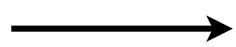
\includegraphics[keepaspectratio]{images/4a92353c5e7c73be482cb1080ea6d63f8cf218a5e63a6ed03e111193d943eb3c.jpg}}

s.set\_shares(50)

\bookmarksetup{startatroot}

\chapter{Properties}\label{properties}

• An alternative approach to accessor methods

class Stock:

\begin{Shaded}
\begin{Highlighting}[]
\KeywordTok{def} \FunctionTok{\_\_init\_\_}\NormalTok{(}\VariableTok{self}\NormalTok{, name, shares, price):}
    \VariableTok{self}\NormalTok{.name }\OperatorTok{=}\NormalTok{ name}
    \VariableTok{self}\NormalTok{.share }\OperatorTok{=}\NormalTok{ shares}
    \VariableTok{self}\NormalTok{.price }\OperatorTok{=}\NormalTok{ price }
\end{Highlighting}
\end{Shaded}

(\textbf{property?})

\begin{Shaded}
\begin{Highlighting}[]
\KeywordTok{def}\NormalTok{ shares(}\VariableTok{self}\NormalTok{):}
    \ControlFlowTok{return} \VariableTok{self}\NormalTok{.\_shares }
\end{Highlighting}
\end{Shaded}

(\textbf{shares.setter?})

\begin{Shaded}
\begin{Highlighting}[]
\KeywordTok{def}\NormalTok{ shares(}\VariableTok{self}\NormalTok{, value): }\ControlFlowTok{if} \KeywordTok{not} \BuiltInTok{isinstance}\NormalTok{(value, }\BuiltInTok{int}\NormalTok{): }\ControlFlowTok{raise} \PreprocessorTok{TypeError}\NormalTok{(}\StringTok{\textquotesingle{}Expected int\textquotesingle{}}\NormalTok{) }\VariableTok{self}\NormalTok{.\_shares }\OperatorTok{=}\NormalTok{ value }
\end{Highlighting}
\end{Shaded}

• The syntax is a little jarring at first

\bookmarksetup{startatroot}

\chapter{Properties}\label{properties-1}

\bookmarksetup{startatroot}

\chapter{• Normal attribute access triggers the
methods}\label{normal-attribute-access-triggers-the-methods}

class Stock:

def \textbf{init}(self, name, shares, price):

self.name \(=\) name

self.shares \(=\) shares

self.price \(=\) price

get \textgreater\textgreater\textgreater{} s = Stock(\ldots)
\textgreater\textgreater\textgreater{} s = Stock(\ldots)
\textgreater\textgreater\textgreater{} s.shares
\textgreater\textgreater\textgreater{} s.shares (\textbf{property?}) 100
100

def shares(self):

return self.\_shares

set

\begin{quote}
\begin{quote}
\begin{quote}
s.shares = 50
\end{quote}
\end{quote}
\end{quote}

\begin{quote}
\begin{quote}
\begin{quote}
\end{quote}
\end{quote}
\end{quote}

(\textbf{shares.setter?})

def shares(self, value):

if not isinstance(value, int):

raise TypeError(`Expected int')

self.\_shares \(=\) value

\bookmarksetup{startatroot}

\chapter{• No changes needed to other source
code}\label{no-changes-needed-to-other-source-code}

\bookmarksetup{startatroot}

\chapter{Properties}\label{properties-2}

• You don't change existing attribute access

class Stock:

def \textbf{init}(self, name, shares, price):

self.shares \(=\) shares

(\textbf{property?})

def shares(self):

return self.\_shares

assignment calls the setter

(\textbf{shares.setter?})

def shares(self, value):

if not isinstance(value, int):

raise TypeError(`Expected int')

self.\_shares \(=\) value

Common confusion: property vs private name

\bookmarksetup{startatroot}

\chapter{Properties}\label{properties-3}

Properties are also useful if you are creating objects where you want to
have a very consistent programming interface\\
Example : Computed data attributes

\begin{Shaded}
\begin{Highlighting}[]
\KeywordTok{class}\NormalTok{ Stock: }\KeywordTok{def} \FunctionTok{\_\_init\_\_}\NormalTok{(}\VariableTok{self}\NormalTok{, name, shares, price): }\VariableTok{self}\NormalTok{.name }\OperatorTok{=}\NormalTok{ name }\VariableTok{self}\NormalTok{.share }\OperatorTok{=}\NormalTok{ shares }\VariableTok{self}\NormalTok{.price }\OperatorTok{=}\NormalTok{ price }\OperatorTok{@}\NormalTok{property }\KeywordTok{def}\NormalTok{ cost(}\VariableTok{self}\NormalTok{): }\ControlFlowTok{return} \VariableTok{self}\NormalTok{.share }\OperatorTok{*} \VariableTok{self}\NormalTok{.price }
\end{Highlighting}
\end{Shaded}

\bookmarksetup{startatroot}

\chapter{Properties}\label{properties-4}

\bookmarksetup{startatroot}

\chapter{• Example use:}\label{example-use}

\begin{Shaded}
\begin{Highlighting}[]
\NormalTok{\textgreater{}\textgreater{}\textgreater{} s = Stock(\textquotesingle{}ACME\textquotesingle{}, 50, 91.1)  }
\NormalTok{\textgreater{}\textgreater{}\textgreater{} s.name Instance Variable  }
\NormalTok{\textquotesingle{}ACME\textquotesingle{}  }
\NormalTok{\textgreater{}\textgreater{}\textgreater{} s.cost Computed Property  }
\NormalTok{4555.0  }
\NormalTok{\textgreater{}\textgreater{}\textgreater{} }
\end{Highlighting}
\end{Shaded}

Commentary : Notice how there is no obvious difference between the
attributes as seen by the user of the object

\bookmarksetup{startatroot}

\chapter{slots Attribute}\label{slots-attribute}

• You can restrict the set of attribute names

\begin{Shaded}
\begin{Highlighting}[]
\KeywordTok{class}\NormalTok{ Stock: }\VariableTok{\_\_slots\_\_} \OperatorTok{=}\NormalTok{ (}\StringTok{\textquotesingle{}name\textquotesingle{}}\NormalTok{, }\StringTok{\textquotesingle{}shares\textquotesingle{}}\NormalTok{, }\StringTok{\textquotesingle{}price\textquotesingle{}}\NormalTok{) ... }
\end{Highlighting}
\end{Shaded}

• Produces errors for other attributes

\begin{Shaded}
\begin{Highlighting}[]
\NormalTok{\textgreater{}\textgreater{}\textgreater{} s = Stock(\textquotesingle{}ACME\textquotesingle{}, 50, 91.1)  }
\NormalTok{\textgreater{}\textgreater{}\textgreater{} s.share = 75  }
\NormalTok{\textgreater{}\textgreater{}\textgreater{} s.share = 75  }
\NormalTok{Traceback (most recent call last):  }
\NormalTok{    File "\textless{}stdin\textgreater{}", line 1, in ?  }
\NormalTok{AttributeError: \textquotesingle{}Stock\textquotesingle{} object has no attribute \textquotesingle{}share\textquotesingle{} }
\end{Highlighting}
\end{Shaded}

This is a performance optimization (uses less memory, runs faster)

\bookmarksetup{startatroot}

\chapter{slots Cautions}\label{slots-cautions}

slots should only be used sparingly\\
Be aware that it's presence can cause strange interaction with other
parts of Python that are related to objects\\
• Advice : Do not use it except with classes that are simply going to
serve as simple data structures

\bookmarksetup{startatroot}

\chapter{Commentary}\label{commentary-1}

The features described so far cover virtually everything that you will
see in most Python class definitions\\
Essential pieces

Instance data (assignment in \textbf{init})\\
Methods (instance, static, class)\\
Properties\\
Private attributes, \_\_slots\_

\bookmarksetup{startatroot}

\chapter{Exercise 3.4}\label{exercise-3.4}

Time : 15 Minutes

\bookmarksetup{startatroot}

\chapter{Inheritance}\label{inheritance}

• A tool for specializing existing objects

class Parent:

class Child(Parent):

• New class called a derived class or subclass\\
Parent known as base class or superclass\\
Parent is specified in () after class name

\bookmarksetup{startatroot}

\chapter{Inheritance}\label{inheritance-1}

• What do you mean by ``specialize?''\\
• Take an existing class and \ldots{}

• Add new methods\\
Redefine some of the existing methods\\
• Add new attributes to instances

In a nutshell: Extending existing code

\bookmarksetup{startatroot}

\chapter{Inheritance Example}\label{inheritance-example}

\bookmarksetup{startatroot}

\chapter{Adding a new method}\label{adding-a-new-method}

class MyStock(Stock): def panic(self): self sell(self.share)\\
\textgreater\textgreater\textgreater s \(\equiv\)
MyStock(`GOOG'，100，490.1)
\textgreater\textgreater\textgreater sSell(25)\\
\textgreater\textgreater\textgreater s.share\\
75\\
\textgreater\textgreater\textgreater s.panic()\\
\textgreater\textgreater\textgreater s.share\\
0\\
\textgreater\textgreater\textgreater{}

\bookmarksetup{startatroot}

\chapter{• You can give new capabilities to existing
objects}\label{you-can-give-new-capabilities-to-existing-objects}

\bookmarksetup{startatroot}

\chapter{Inheritance Example}\label{inheritance-example-1}

\bookmarksetup{startatroot}

\chapter{Redefining a method}\label{redefining-a-method}

class MyStock(Stock): def cost(self): return 1.25 * self.share *
self.price\\
\textgreater\textgreater\textgreater s \(=\)
MyStock(`GOOG'，100，490.1)\\
\textgreater\textgreater\textgreater s.cost()\\
61262.5\\
\textgreater\textgreater\textgreater{}

• The new method takes the place of the old one\\
• Other methods are unaffected

\bookmarksetup{startatroot}

\chapter{Inheritance and Overriding}\label{inheritance-and-overriding}

Sometimes a class extends an existing method, but it has to use the
original implementation

class Stock: def cost(self): return self.share * self.price class
MyStock(Stock): def cost(self): actual\_cost \(=\) super().cost() return
1.25 * actual\_cost

• Use super() to call previous version\\
Caution: Python 2 is different

actual\_cost \(=\) super(MyStock, self).cost()

\bookmarksetup{startatroot}

\chapter{Inheritance and init}\label{inheritance-and-init}

• With inheritance, you must initialize parents

class Stock:

def \textbf{init}(self, name, shares, price):

self.name \(=\) name

self.shares \(=\) shares

self.price \(=\) price

class MyStock(Stock):

def \textbf{init}(self, name, shares, price, factor):

super().\_\_init\_\_(name, shares, price)

self.factor \(=\) factor

def cost(self):

return self.factor * super().cost()

• Again, you should use super() as shown

\bookmarksetup{startatroot}

\chapter{I: is a'' relationship}\label{i-is-a-relationship}

• Inheritance establishes a type relationship

class Stock:\\
class MyStock(Stock):\\
\textgreater\textgreater\textgreater s \(\equiv\)
MyStock(`ACME'，50，91.1)
\textgreater\textgreater\textgreater isinstance(s，Stock) True\\
\textgreater\textgreater\textgreater{}

Important: objects defined via inheritance are a special version of the
parent (same capabilities)

\bookmarksetup{startatroot}

\chapter{object base class}\label{object-base-class}

Sometimes a class will use object as parent

class Stock(object):

object is the parent of all objects in Python (even if you don't specify
it in Python 3)\\
Note: There is some historical baggage with Python 2 so it's common to
see it in old code

\bookmarksetup{startatroot}

\chapter{Multiple Inheritance}\label{multiple-inheritance}

• You can specify multiple base classes

\begin{Shaded}
\begin{Highlighting}[]
\KeywordTok{class}\NormalTok{ Parent1:   }
\NormalTok{...   }
\KeywordTok{class}\NormalTok{ Parent2:   }
\NormalTok{...   }
\KeywordTok{class}\NormalTok{ Child(Parent1,Parent2): }
\end{Highlighting}
\end{Shaded}

• The new class inherits features from both parents\\
But there are some really tricky details (later)\\
• Don't do it unless you understand it

\bookmarksetup{startatroot}

\chapter{Using Inheritance}\label{using-inheritance}

Inheritance is often used as a code customization/extensibility
feature\\
For example, certain parts of a framework might involve inheriting from
an existing class and redefining a handful of methods\\
• Idea: you add bits and pieces to existing code to make it do custom
processing

\bookmarksetup{startatroot}

\chapter{Exercise 3.5}\label{exercise-3.5}

Time : 20 Minutes

\bookmarksetup{startatroot}

\chapter{Special Methods}\label{special-methods}

• Classes can customize almost every aspect of their behavior\\
This is done through special methods

\begin{Shaded}
\begin{Highlighting}[]
\KeywordTok{class}\NormalTok{ Point: }\KeywordTok{def} \FunctionTok{\_\_init\_\_}\NormalTok{(}\VariableTok{self}\NormalTok{, x, y): ... }\KeywordTok{def} \FunctionTok{\_\_str\_\_}\NormalTok{(}\VariableTok{self}\NormalTok{): }
\end{Highlighting}
\end{Shaded}

• There are dozens of these methods\\
Instead of showing every possible customization, will show essential
ones

\bookmarksetup{startatroot}

\chapter{String Conversions}\label{string-conversions}

• Objects have two string representations

\begin{Shaded}
\begin{Highlighting}[]
\NormalTok{\textgreater{}\textgreater{}\textgreater{} from datetime import date  }
\NormalTok{\textgreater{}\textgreater{}\textgreater{} d = date(2012, 12, 21)  }
\NormalTok{\textgreater{}\textgreater{}\textgreater{} print(d)  }
\NormalTok{2012{-}12{-}21  }
\NormalTok{\textgreater{}\textgreater{}\textgreater{} d  }
\NormalTok{datetime.date(2012, 12, 21)  }
\NormalTok{\textgreater{}\textgreater{}\textgreater{} }
\end{Highlighting}
\end{Shaded}

str(x) - Printable output \textgreater\textgreater\textgreater{} str(d)
`2012-12-21' \textgreater\textgreater\textgreater{}\\
repr(x) - For programmers \textgreater\textgreater\textgreater{} repr(d)
`datetime.date(2012, 12, 21)' \textgreater\textgreater\textgreater{}

\bookmarksetup{startatroot}

\chapter{String Conversions}\label{string-conversions-1}

class Date:

\begin{Shaded}
\begin{Highlighting}[]
\KeywordTok{def} \FunctionTok{\_\_init\_\_}\NormalTok{(}\VariableTok{self}\NormalTok{, year, month, day):}
    \VariableTok{self}\NormalTok{.year }\OperatorTok{=}\NormalTok{ year}
    \VariableTok{self}\NormalTok{.month }\OperatorTok{=}\NormalTok{ month}
    \VariableTok{self}\NormalTok{.day }\OperatorTok{=}\NormalTok{ day }
\end{Highlighting}
\end{Shaded}

\begin{Shaded}
\begin{Highlighting}[]
\KeywordTok{def} \FunctionTok{\_\_str\_\_}\NormalTok{(}\VariableTok{self}\NormalTok{):}
    \ControlFlowTok{return} \StringTok{\textquotesingle{}d{-}}\SpecialCharTok{\%d}\StringTok{{-}}\SpecialCharTok{\%d}\StringTok{\textquotesingle{}} \OperatorTok{\%}\NormalTok{ (}\VariableTok{self}\NormalTok{.year, }\VariableTok{self}\NormalTok{.month, }\VariableTok{self}\NormalTok{.day) }
\end{Highlighting}
\end{Shaded}

\begin{Shaded}
\begin{Highlighting}[]
\KeywordTok{def} \FunctionTok{\_\_repr\_\_}\NormalTok{(}\VariableTok{self}\NormalTok{):}
    \ControlFlowTok{return} \StringTok{\textquotesingle{}Date(}\SpecialCharTok{\%r}\StringTok{,}\SpecialCharTok{\%r}\StringTok{,}\SpecialCharTok{\%r}\StringTok{)\textquotesingle{}} \OperatorTok{\%}\NormalTok{ (}\VariableTok{self}\NormalTok{.year, }\VariableTok{self}\NormalTok{.month, }\VariableTok{self}\NormalTok{.day) }
\end{Highlighting}
\end{Shaded}

Note: The convention for \textbf{repr}() is to return a string that,
when fed to eval() , will recreate the underlying object. If this is not
possible, some kind of easily readable representation is used instead.

\bookmarksetup{startatroot}

\chapter{Methods: Item Access}\label{methods-item-access}

• Methods used to implement containers

\begin{Shaded}
\begin{Highlighting}[]
\NormalTok{len(x) x.\_len\_(x[a] x.\_getitem\_(a)  }
\NormalTok{x[a] = v x.\_setitem\_(a,v)  }
\NormalTok{del x[a] x.\_delitem\_(a)  }
\NormalTok{a in x x.\_contains\_(a) }
\end{Highlighting}
\end{Shaded}

Definition in a class

\begin{Shaded}
\begin{Highlighting}[]
\KeywordTok{class}\NormalTok{ Container: }\KeywordTok{def} \FunctionTok{\_\_len\_\_}\NormalTok{(}\VariableTok{self}\NormalTok{): }\KeywordTok{def} \FunctionTok{\_\_getitem\_\_}\NormalTok{(}\VariableTok{self}\NormalTok{,a): }\KeywordTok{def} \FunctionTok{\_\_setitem\_\_}\NormalTok{(}\VariableTok{self}\NormalTok{,a,v): }\KeywordTok{def} \FunctionTok{\_\_delitem\_\_}\NormalTok{(}\VariableTok{self}\NormalTok{,a): }\KeywordTok{def} \FunctionTok{\_\_contains\_\_}\NormalTok{(}\VariableTok{self}\NormalTok{,a): }
\end{Highlighting}
\end{Shaded}

\bookmarksetup{startatroot}

\chapter{Methods: Mathematics}\label{methods-mathematics}

\bookmarksetup{startatroot}

\chapter{Mathematical operators}\label{mathematical-operators}

a + b a.\_\_add\_\_(b)\\
a - b a.\_\_sub\_\_(b)\\
a * b a.\_\_mul\_\_(b)\\
a / b a.\_\_div\_\_(b)\\
a // b a.\_\_floordiv\_\_(b)\\
a \% b a.\_\_mod\_\_(b)\\
a \textless\textless{} b a.\_\_lshift\_\_(b)\\
a \textgreater\textgreater{} b a.\_\_rshift\_\_(b)\\
a \& b a.\_\_and\_\_(b)\\
a \textbar{} b a.\_\_or\_\_(b)\\
a \^{} b a.\_\_xor\_\_(b)\\
a ** b a.\_\_pow\_\_(b)\\
-a a.\_\_neg\_\_()\\
\textasciitilde a a.\_\_invert\_\_()\\
abs(a) a.\_\_abs\_\_()

\bookmarksetup{startatroot}

\chapter{• Consult reference for further
details}\label{consult-reference-for-further-details}

\bookmarksetup{startatroot}

\chapter{Instance Creation}\label{instance-creation}

Instances are created in two steps

class Date:

def \textbf{init}(self, year, month, day):

self.year = year

self.month \(=\) month

self.day \(=\) day

d = Date(2012, 12, 21)

Under the hood

d = Date.\_\_new\_\_(Date, 2012, 12, 21)

d.\_\_init\_\_(2012, 12, 21)

\bookmarksetup{startatroot}

\chapter{Using new}\label{using-new}

• Sometimes you might use \textbf{new}() directly

class Date:

\begin{Shaded}
\begin{Highlighting}[]
\NormalTok{...}
\AttributeTok{@classmethod}
\KeywordTok{def}\NormalTok{ today(cls):}
\NormalTok{    t }\OperatorTok{=}\NormalTok{ time.localtime()}
    \VariableTok{self} \OperatorTok{=}\NormalTok{ cls.\_new\_\_(cls)}
    \VariableTok{self}\NormalTok{.year }\OperatorTok{=}\NormalTok{ t.tm\_year}
    \VariableTok{self}\NormalTok{.month }\OperatorTok{=}\NormalTok{ t.tm\_mon}
    \VariableTok{self}\NormalTok{.day }\OperatorTok{=}\NormalTok{ t.tm\_mday}
    \ControlFlowTok{return} \VariableTok{self} 
\end{Highlighting}
\end{Shaded}

\begin{Shaded}
\begin{Highlighting}[]
\NormalTok{d = Date today() }
\end{Highlighting}
\end{Shaded}

• Creates an instance, but bypasses \textbf{init}()

\bookmarksetup{startatroot}

\chapter{Defining new}\label{defining-new}

Classes may define \textbf{new}() C

\begin{Shaded}
\begin{Highlighting}[]
\KeywordTok{class}\NormalTok{ A: }\OperatorTok{@}\NormalTok{staticmethod }\KeywordTok{def} \FunctionTok{\_\_new\_\_}\NormalTok{(cls, x, y): }\ControlFlowTok{return} \BuiltInTok{super}\NormalTok{().}\FunctionTok{\_\_new\_\_}\NormalTok{(cls) }\KeywordTok{def} \FunctionTok{\_\_init\_\_}\NormalTok{(}\VariableTok{self}\NormalTok{, x, y): }
\end{Highlighting}
\end{Shaded}

• Not common, but sometimes used when altering some tricky aspect of
instance creation

Instance caching\\
Immutability

\bookmarksetup{startatroot}

\chapter{del method}\label{del-method}

• Classes might define a ``destructor'' method

class Connection:

\begin{Shaded}
\begin{Highlighting}[]
\KeywordTok{def} \FunctionTok{\_\_del\_\_}\NormalTok{(}\VariableTok{self}\NormalTok{):}
    \CommentTok{\# Cleanup statements }
\end{Highlighting}
\end{Shaded}

• Called when the reference count reaches 0\\
• Confusion: Not related to ``del'' operator

\(\mathbf{c} = \mathbf{\text{Con}}\) nnection() \#refcnt \(= 1\) d=c \#
refcnt \(= 2\)

\begin{Shaded}
\begin{Highlighting}[]
\KeywordTok{del}\NormalTok{ d }\CommentTok{\# Doesn\textquotesingle{}t call d.\_del\_( (refcnt = 1)  }
\NormalTok{c }\OperatorTok{=} \VariableTok{None} \CommentTok{\# Calls c.\_del\_( (refcnt = 0) }
\end{Highlighting}
\end{Shaded}

\bookmarksetup{startatroot}

\chapter{del method}\label{del-method-1}

Typical uses:\\
Proper shutdown of system resources (e.g., network connections)\\
• Releasing locks (e.g., threading)\\
• Avoid defining it for any other purpose

\bookmarksetup{startatroot}

\chapter{Weak References}\label{weak-references}

• A weak reference is a reference to an object that does not increase
its reference count\\
Sometimes this is desired in when there is a complicated relationship
between objects and there are issues with memory management\\
Supported by weakref library module

\bookmarksetup{startatroot}

\chapter{weakref module}\label{weakref-module}

Creating a weak reference

\begin{Shaded}
\begin{Highlighting}[]
\OperatorTok{\textgreater{}\textgreater{}\textgreater{}} \ImportTok{import}\NormalTok{ weakref}
\OperatorTok{\textgreater{}\textgreater{}\textgreater{}}\NormalTok{ f }\OperatorTok{=}\NormalTok{ Foo()}
\OperatorTok{\textgreater{}\textgreater{}\textgreater{}}\NormalTok{ ref }\OperatorTok{=}\NormalTok{ weakref.ref(f)}
\OperatorTok{\textgreater{}\textgreater{}\textgreater{}}\NormalTok{ ref}
\OperatorTok{\textless{}}\NormalTok{weakref at }\BaseNTok{0x4203c0}\OperatorTok{;}\NormalTok{ to }\StringTok{\textquotesingle{}Foo\textquotesingle{}}\NormalTok{ at }\BaseNTok{0x41cff0}\OperatorTok{\textgreater{}} 
\end{Highlighting}
\end{Shaded}

• Getting the object being pointed at

\begin{Shaded}
\begin{Highlighting}[]
\NormalTok{\textgreater{}\textgreater{}\textgreater{} g = ref() \# Dereference  }
\NormalTok{\textgreater{}\textgreater{}\textgreater{} print(g)  }
\NormalTok{\textless{}\_\_main\_\_.Foo object at 0x41dfff0\textgreater{} }
\end{Highlighting}
\end{Shaded}

• If object is dead, deference returns None

\begin{Shaded}
\begin{Highlighting}[]
\NormalTok{\textgreater{}\textgreater{}\textgreater{} g = freq()  }
\NormalTok{\textgreater{}\textgreater{}\textgreater{} print(g)  }
\NormalTok{None }
\end{Highlighting}
\end{Shaded}

\bookmarksetup{startatroot}

\chapter{Using Weak References}\label{using-weak-references}

Weak references are sometimes used where there are reference cycles
between objects\\
Example : graphs, trees, observers, caches,etc.\\
Not something you should consider unless dealing with really tricky
memory problems\\
• More features in the weakref module

\bookmarksetup{startatroot}

\chapter{Context Managers}\label{context-managers}

For resources, consider the use of the `with' statement instead of
relying on \textbf{del}()

\begin{Shaded}
\begin{Highlighting}[]
\NormalTok{with obj as val: val = obj.\_\_enter\_\_(  ) statements statements statements statements statements obj.\_exit\_(ty, val, tb) }
\end{Highlighting}
\end{Shaded}

• Allows you to customize entry/exit steps

\bookmarksetup{startatroot}

\chapter{Context Managers}\label{context-managers-1}

\bookmarksetup{startatroot}

\chapter{Example:}\label{example}

\begin{Shaded}
\begin{Highlighting}[]
\KeywordTok{class}\NormalTok{ Manager: }\KeywordTok{def} \FunctionTok{\_\_enter\_\_}\NormalTok{(}\VariableTok{self}\NormalTok{): }\BuiltInTok{print}\NormalTok{(}\StringTok{\textquotesingle{}Entering\textquotesingle{}}\NormalTok{) }\ControlFlowTok{return} \VariableTok{self} \KeywordTok{def} \FunctionTok{\_\_exit\_\_}\NormalTok{(}\VariableTok{self}\NormalTok{,ty，val，tb): }\BuiltInTok{print}\NormalTok{(}\StringTok{\textquotesingle{}Leaving\textquotesingle{}}\NormalTok{) }\ControlFlowTok{if}\NormalTok{ ty: }\BuiltInTok{print}\NormalTok{(}\StringTok{\textquotesingle{}An exception occurred\textquotesingle{}}\NormalTok{) }
\end{Highlighting}
\end{Shaded}

\bookmarksetup{startatroot}

\chapter{• Example use:}\label{example-use-1}

\begin{Shaded}
\begin{Highlighting}[]
\NormalTok{\textgreater{}\textgreater{}\textgreater{} m = Manager()}
\NormalTok{\textgreater{}\textgreater{}\textgreater{} with m:}
\NormalTok{...}
\NormalTok{...}
\NormalTok{print(\textquotesingle{}Hello World\textquotesingle{})}
\NormalTok{...}
\NormalTok{Entering}
\NormalTok{Hello World}
\NormalTok{Leaving}
\NormalTok{\textgreater{}\textgreater{}\textgreater{} }
\end{Highlighting}
\end{Shaded}

Note: the ty, val, tb arguments have information about pending
exceptions (if any)

\bookmarksetup{startatroot}

\chapter{Exercise 3.6}\label{exercise-3.6}

Time : 15 Minutes

\bookmarksetup{startatroot}

\chapter{Code Reuse}\label{code-reuse}

• A major theme of object oriented programming concerns code reuse and
making things extensible\\
A big topic\\
• There are a number of common techniques

\bookmarksetup{startatroot}

\chapter{Interfaces}\label{interfaces}

Classes often serve as a kind of design specification or programming
interface

\begin{Shaded}
\begin{Highlighting}[]
\KeywordTok{class}\NormalTok{ IStream: }\KeywordTok{def}\NormalTok{ read(}\VariableTok{self}\NormalTok{, maxbytes}\OperatorTok{=}\VariableTok{None}\NormalTok{): }\ControlFlowTok{raise} \PreprocessorTok{NotImplementedError}\NormalTok{(): }\KeywordTok{def}\NormalTok{ write(}\VariableTok{self}\NormalTok{, data): }\ControlFlowTok{raise} \PreprocessorTok{NotImplementedError}\NormalTok{() }
\end{Highlighting}
\end{Shaded}

This class isn't used directly, but is usually included as a base class
for other objects

\begin{Shaded}
\begin{Highlighting}[]
\KeywordTok{class}\NormalTok{ UnixPipe(IStream): }\KeywordTok{def}\NormalTok{ read(}\VariableTok{self}\NormalTok{, maxbytes}\OperatorTok{=}\VariableTok{None}\NormalTok{): }\KeywordTok{def}\NormalTok{ write(}\VariableTok{self}\NormalTok{, data): }
\end{Highlighting}
\end{Shaded}

\bookmarksetup{startatroot}

\chapter{Abstract Base Classes}\label{abstract-base-classes}

Consider defining interfaces as an abstract base class (ABC) instead

from abc import ABC, abstractmethod

\begin{Shaded}
\begin{Highlighting}[]
\KeywordTok{class}\NormalTok{ IStream(ABC):}
    \AttributeTok{@abstractmethod}
        \KeywordTok{def}\NormalTok{ read(}\VariableTok{self}\NormalTok{, maxbytes}\OperatorTok{=}\VariableTok{None}\NormalTok{):}
            \ControlFlowTok{pass}
        \AttributeTok{@abstractmethod}
            \KeywordTok{def}\NormalTok{ write(}\VariableTok{self}\NormalTok{, data):}
                \ControlFlowTok{pass} 
\end{Highlighting}
\end{Shaded}

Doesn't allow instantiation unless all of the abstract methods have been
fully implemented

\bookmarksetup{startatroot}

\chapter{Abstract Base Classes}\label{abstract-base-classes-1}

• ABCs may simplify type checking

\begin{Shaded}
\begin{Highlighting}[]
\KeywordTok{def}\NormalTok{ write\_data(data, stream):}
    \ControlFlowTok{if} \KeywordTok{not} \BuiltInTok{isinstance}\NormalTok{(stream, IStream):}
        \ControlFlowTok{raise} \PreprocessorTok{TypeError}\NormalTok{(}\StringTok{\textquotesingle{}Expected a Stream\textquotesingle{}}\NormalTok{) }
\end{Highlighting}
\end{Shaded}

• ABCs catch careless usage errors

\begin{Shaded}
\begin{Highlighting}[]
\KeywordTok{class}\NormalTok{ UnixPipe(IStream): }\KeywordTok{def}\NormalTok{ recv(}\VariableTok{self}\NormalTok{, maxbytes}\OperatorTok{=}\VariableTok{None}\NormalTok{): }\KeywordTok{def}\NormalTok{ write(}\VariableTok{self}\NormalTok{, data): }\ControlFlowTok{pass} \OperatorTok{\textgreater{}\textgreater{}\textgreater{}}\NormalTok{ p }\OperatorTok{=}\NormalTok{ UnixPipe() Traceback (most recent call last): File }\StringTok{"\textless{}stdin\textgreater{}"}\NormalTok{, line }\DecValTok{1}\NormalTok{, }\KeywordTok{in} \OperatorTok{\textless{}}\NormalTok{module}\OperatorTok{\textgreater{}} \PreprocessorTok{ValueError}\NormalTok{: Can}\StringTok{\textquotesingle{}t instantiate abstract class UnixPipe with abstract methods read \textgreater{}\textgreater{}\textgreater{} }
\end{Highlighting}
\end{Shaded}

\bookmarksetup{startatroot}

\chapter{Handler Classes}\label{handler-classes}

Sometimes code will implement a general purpose algorithm, but will
defer certain steps to a separately supplied handler object\\
Sometimes known as the ``strategy'' design pattern.

\bookmarksetup{startatroot}

\chapter{Handler Classes}\label{handler-classes-1}

\bookmarksetup{startatroot}

\chapter{• Example :}\label{example-1}

def print\_table(record, fields,formatter):\\
Calls to\\
handler\\
methods for r in records: rowdata \(=\) {[}getattr(r, fieldname,`undef')
for fieldname in fields{]} \(\rightarrow\) formatter(row(rowdata)

Notice how various steps of the algorithm are deferred to a separate
handler object

\bookmarksetup{startatroot}

\chapter{Handler Classes}\label{handler-classes-2}

• Handlers have their own class definition

class TableFormatter: def headings(self, headings): raise
NotImplementedError def row(self, rowdata): raise NotImplementedError

The handler only contains the methods that need to be
implemented/customized\\
Important idea : Decoupling of the class that produces the table from
the handler methods

\bookmarksetup{startatroot}

\chapter{Handler Classes}\label{handler-classes-3}

\bookmarksetup{startatroot}

\chapter{Example Use}\label{example-use-2}

\begin{Shaded}
\begin{Highlighting}[]
\KeywordTok{class}\NormalTok{ TextTableFormatter(TableFormatter): }\KeywordTok{def}\NormalTok{ headings(}\VariableTok{self}\NormalTok{, headers): }\ControlFlowTok{for}\NormalTok{ h }\KeywordTok{in}\NormalTok{ headers: }\BuiltInTok{print}\NormalTok{(}\StringTok{\textquotesingle{}}\SpecialCharTok{\%10s}\StringTok{\textquotesingle{}} \OperatorTok{\%}\NormalTok{ h, end}\OperatorTok{=}\StringTok{\textquotesingle{}\textquotesingle{}}\NormalTok{) }\BuiltInTok{print}\NormalTok{() }\BuiltInTok{print}\NormalTok{(}\StringTok{\textquotesingle{}{-}*10+\textquotesingle{}} \OperatorTok{*} \BuiltInTok{len}\NormalTok{(columns)) }\KeywordTok{def}\NormalTok{ row(}\VariableTok{self}\NormalTok{, rowdata): }\ControlFlowTok{for}\NormalTok{ d }\KeywordTok{in}\NormalTok{ rowdata: }\BuiltInTok{print}\NormalTok{(}\StringTok{\textquotesingle{}}\SpecialCharTok{\%10s}\StringTok{\textquotesingle{}} \OperatorTok{\%}\NormalTok{ d, end}\OperatorTok{=}\StringTok{\textquotesingle{}\textquotesingle{}}\NormalTok{) }\BuiltInTok{print}\NormalTok{() }
\end{Highlighting}
\end{Shaded}

\begin{Shaded}
\begin{Highlighting}[]
\NormalTok{formatter }\OperatorTok{=}\NormalTok{ TextTableFormatter()}
\NormalTok{print\_table笑着说, [}\StringTok{\textquotesingle{}name\textquotesingle{}}\NormalTok{, }\StringTok{\textquotesingle{}shares\textquotesingle{}}\NormalTok{],formatter) }
\end{Highlighting}
\end{Shaded}

\bookmarksetup{startatroot}

\chapter{Commentary}\label{commentary-2}

The use of handler classes is extremely common throughout the Python
standard library (might be the most popular OO design pattern used in
Python)\\
Rationale : This approach provides flexibility\\
• Handlers are decoupled from implementation\\
• Allows handler code to be reused in other contexts (other classes can
use the same handler objects).

\bookmarksetup{startatroot}

\chapter{Classes as a Template}\label{classes-as-a-template}

• A class might implement a generalpurpose algorithm, but delegate
certain steps to a subclass\\
• Will illustrate with a simple example

\bookmarksetup{startatroot}

\chapter{Template Example}\label{template-example}

• A class that parses a CSV file into a list

class CSVParser: def parse(self, filename): records \(=\) {[}{]} with
open(filename) as f: rows \(=\) csv-reader(f) self Headers \(=\)
nextrows) for row in rows: record \(=\) self.make\_record(row)
records.append(record) return records

\begin{Shaded}
\begin{Highlighting}[]
\NormalTok{Step that must be implemented }\KeywordTok{def}\NormalTok{ make\_record(}\VariableTok{self}\NormalTok{, row): raiseRuntimeError(}\StringTok{\textquotesingle{}Must implement\textquotesingle{}}\NormalTok{) }
\end{Highlighting}
\end{Shaded}

• Note: Class is useless by itself

\bookmarksetup{startatroot}

\chapter{Template Example}\label{template-example-1}

• Using the template (use inheritance)

\begin{Shaded}
\begin{Highlighting}[]
\KeywordTok{class}\NormalTok{ DictCSVParser(CSVParser): defmake\_record(}\VariableTok{self}\NormalTok{,row): returndict(}\BuiltInTok{zip}\NormalTok{(}\VariableTok{self}\NormalTok{.headers,row)) }
\end{Highlighting}
\end{Shaded}

parser \(=\) DictCSVParser()\\
portfolio \(\equiv\) parser.parse(`portfolio.csv')

Critical idea : User defines a small class that supplies the one missing
piece, but most of the real functionality is in the base class

\bookmarksetup{startatroot}

\chapter{Prefer Functions}\label{prefer-functions}

• The template pattern is often overcomplicated\\
• Consider a function + callback instead

\begin{Shaded}
\begin{Highlighting}[]
\KeywordTok{def}\NormalTok{ parse\_csv(filename, make\_record): records }\OperatorTok{=}\NormalTok{ [] }\ControlFlowTok{with} \BuiltInTok{open}\NormalTok{(filename) }\ImportTok{as}\NormalTok{ f: rows }\OperatorTok{=}\NormalTok{ csv}\OperatorTok{{-}}\NormalTok{reader(f) headers }\OperatorTok{=} \BuiltInTok{next}\NormalTok{(rows) }\ControlFlowTok{for}\NormalTok{ row }\KeywordTok{in}\NormalTok{ rows: record }\OperatorTok{=}\NormalTok{ make\_record(headers, row) records.append(record) }\ControlFlowTok{return}\NormalTok{ records }
\end{Highlighting}
\end{Shaded}

\begin{Shaded}
\begin{Highlighting}[]
\KeywordTok{def}\NormalTok{ make\_record(headers, row):}
    \CommentTok{\# User implements }
\end{Highlighting}
\end{Shaded}

\bookmarksetup{startatroot}

\chapter{Exercise 3.7}\label{exercise-3.7}

Time : 15 Minutes

\bookmarksetup{startatroot}

\chapter{Advanced Inheritance}\label{advanced-inheritance}

Recall: Inheritance is a tool for code reuse (customization and
extension)

\begin{Shaded}
\begin{Highlighting}[]
\KeywordTok{class}\NormalTok{ Parent: }\KeywordTok{def}\NormalTok{ spam(}\VariableTok{self}\NormalTok{): }\KeywordTok{class}\NormalTok{ Child(Parent): }\KeywordTok{def}\NormalTok{ spam(}\VariableTok{self}\NormalTok{): }\BuiltInTok{print}\NormalTok{(}\StringTok{\textquotesingle{}Different spam\textquotesingle{}}\NormalTok{) }\BuiltInTok{super}\NormalTok{().spam() }
\end{Highlighting}
\end{Shaded}

• Child classes can customize their parents\\
• Sometimes see use of super() function (shown)

\bookmarksetup{startatroot}

\chapter{Multiple Inheritance}\label{multiple-inheritance-1}

Classes can have multiple parents

\pandocbounded{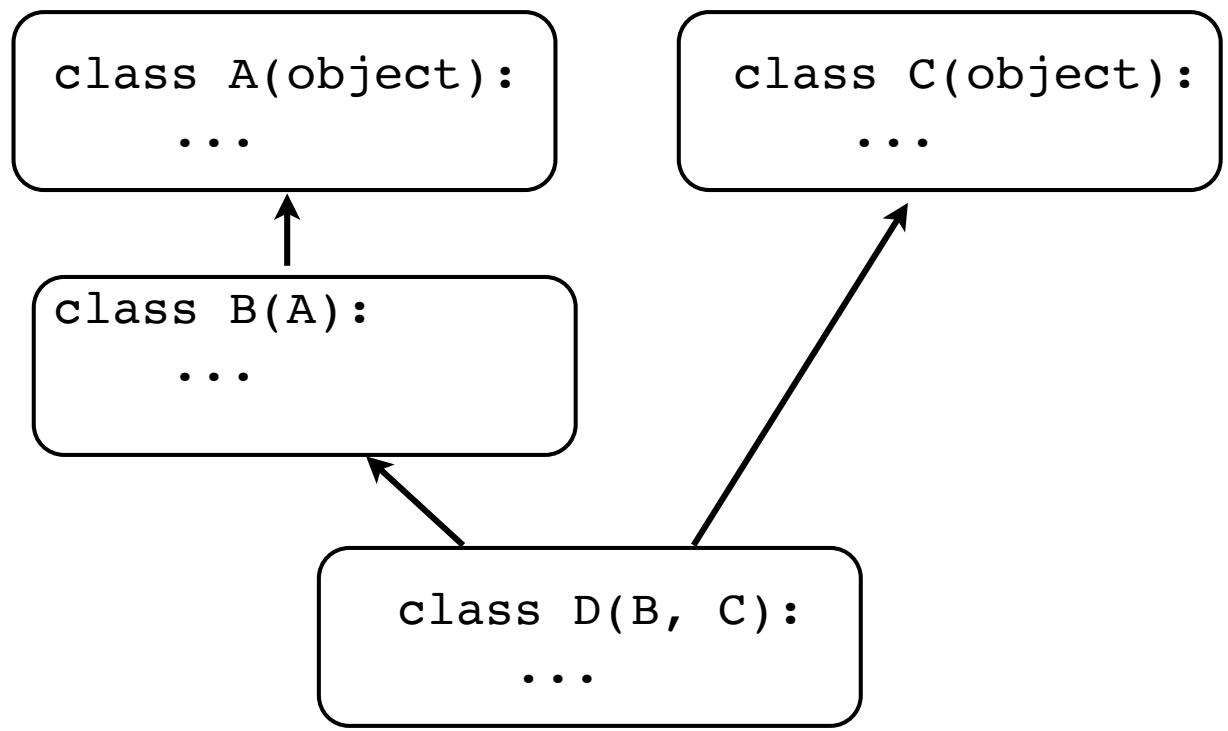
\includegraphics[keepaspectratio]{images/7a890f0f00233cb3ae414d9e8707512c7bb6cac44651ffdbb88a48375a329c97.jpg}}

• The child will inherit features from all parents\\
But, it's a lot sneakier than this

\bookmarksetup{startatroot}

\chapter{Cooperative Inheritance}\label{cooperative-inheritance}

Python uses ``cooperative multiple inheritance''\\
Big idea: A child class can specifically arrange its parents to
cooperate with each other

class Child(Parent1, Parent2, Parent3):

The order of the parents has significance\\
• Attribute search may jump parent-to-parent

\pandocbounded{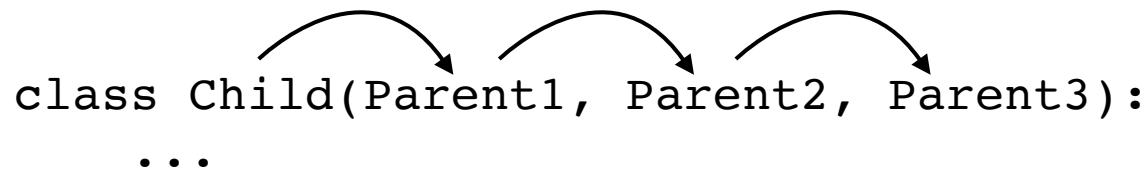
\includegraphics[keepaspectratio]{images/65cdbb8bd74ddce9296c917c14d529dae8ebce2f10aeb6d2e60b0ee6b3ee2bde.jpg}}

\bookmarksetup{startatroot}

\chapter{Cooperative Inheritance}\label{cooperative-inheritance-1}

• Example: Consider this arrangement

\pandocbounded{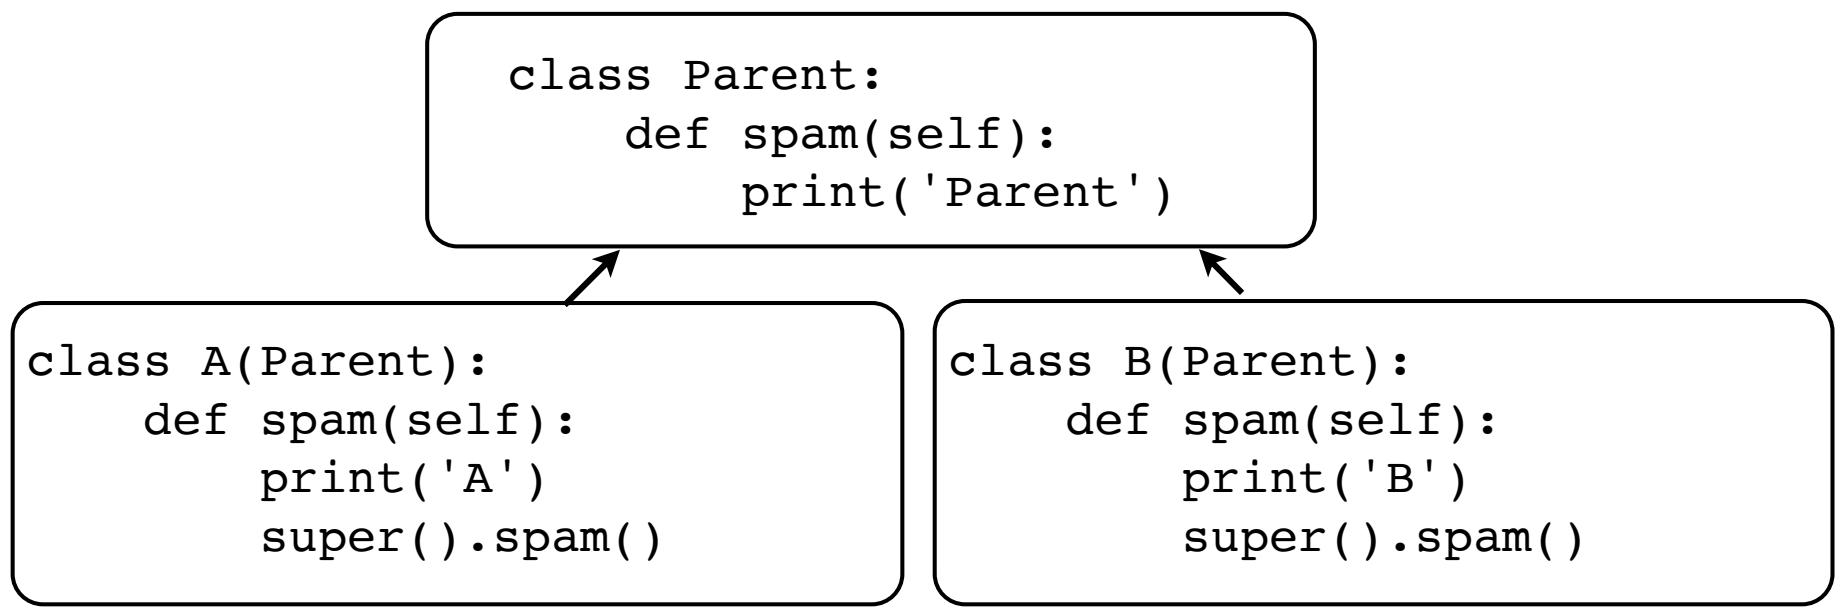
\includegraphics[keepaspectratio]{images/62a05ad300f082d7671e00233e36563c2b040faf31205586f1fe2bc0dad5cd4f.jpg}}

• Now, this:

\pandocbounded{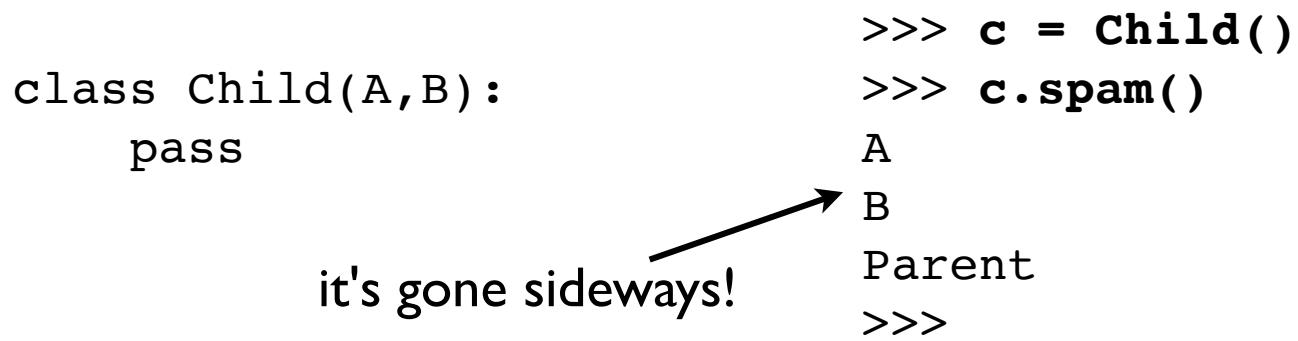
\includegraphics[keepaspectratio]{images/1bd9570cf2d038c58720a0ee5e01bf17cc873dbf6de8238123aadc459a8b6ebe.jpg}}

\bookmarksetup{startatroot}

\chapter{Cooperative Inheritance}\label{cooperative-inheritance-2}

There are applications

\pandocbounded{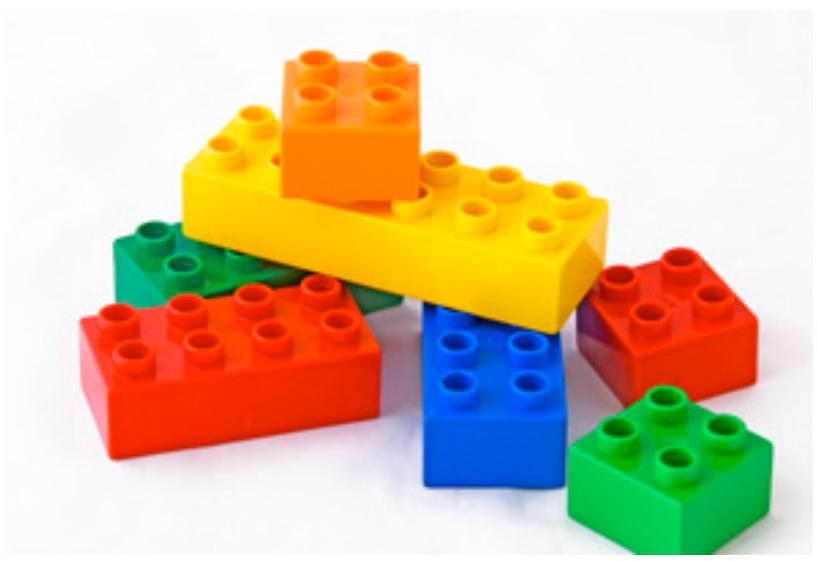
\includegraphics[keepaspectratio]{images/cb9fa28655840657c43986c68d98e0d268152d3d5e1ad86f3d547934e4244ec0.jpg}}

You can make collections of classes that are meant to be stacked
together to make more interesting things

\bookmarksetup{startatroot}

\chapter{An Odd Code Reuse}\label{an-odd-code-reuse}

\begin{Shaded}
\begin{Highlighting}[]
\KeywordTok{class}\NormalTok{ Dog: }\KeywordTok{def}\NormalTok{ noise(}\VariableTok{self}\NormalTok{): }\ControlFlowTok{return} \StringTok{\textquotesingle{}Woof\textquotesingle{}} \KeywordTok{def}\NormalTok{ chase(}\VariableTok{self}\NormalTok{): }\ControlFlowTok{return} \StringTok{\textquotesingle{}Chasing!\textquotesingle{}}   
\KeywordTok{class}\NormalTok{ LoudDog(Dog): }\KeywordTok{def}\NormalTok{ noise(}\VariableTok{self}\NormalTok{): }\ControlFlowTok{return} \BuiltInTok{super}\NormalTok{()\textbackslash{} .noise().upper() }
\end{Highlighting}
\end{Shaded}

\begin{Shaded}
\begin{Highlighting}[]
\NormalTok{class Bike: def noise(self): return \textquotesingle{}On Your Left\textquotesingle{} def pedal(self): return \textquotesingle{}Pedaling!\textquotesingle{} class LoudBike(Bike): def noise(self): return super()\textbackslash{} .noise().upper() }
\end{Highlighting}
\end{Shaded}

Completely unrelated objects\\
But, there is a code commonality

\bookmarksetup{startatroot}

\chapter{Mixin Classes}\label{mixin-classes}

A mixin is a class whose purpose is to add extra functionality to other
class definitions\\
• Idea : If a user implements some basic features in their class, a
mixin can be used to fill out the class with extra functionality\\
• Sometimes used as a technique for reducing the amount of code that
must be written

\bookmarksetup{startatroot}

\chapter{Mixin Example}\label{mixin-example}

• A class with a fragment of code

class Loud:

def noise(self):

return super().noise().upper()

Not usable in isolation\\
• Mixes with other classes via inheritance

class LoudDog(Loud, Dog): pass

class LoudBike(Loud, Bike): pass

\bookmarksetup{startatroot}

\chapter{How it works}\label{how-it-works}

Example:

\begin{Shaded}
\begin{Highlighting}[]
\KeywordTok{class}\NormalTok{ LoudDog(Loud, Dog):}
    \ControlFlowTok{pass} \BuiltInTok{super}\NormalTok{() }
\end{Highlighting}
\end{Shaded}

\begin{Shaded}
\begin{Highlighting}[]
\NormalTok{\textgreater{}\textgreater{}\textgreater{}d = LoudDog() }
\end{Highlighting}
\end{Shaded}

\begin{Shaded}
\begin{Highlighting}[]
\NormalTok{\textgreater{}\textgreater{}\textgreater{} d.noise() }
\end{Highlighting}
\end{Shaded}

\begin{Shaded}
\begin{Highlighting}[]
\NormalTok{\textquotesingle{}WOOF\textquotesingle{} }
\end{Highlighting}
\end{Shaded}

\begin{Shaded}
\begin{Highlighting}[]
\NormalTok{\textgreater{}\textgreater{}\textgreater{} }
\end{Highlighting}
\end{Shaded}

• super() moves to the next class\\
• Allows mixins to combine with arbitrary classes

\bookmarksetup{startatroot}

\chapter{Use of Mixins}\label{use-of-mixins}

Mixin classes are sometimes used as a way to add optional features to
more basic objects\\
For example, added thread support, persistence, etc.\\
User assembles an object from the different parts that they're going to
use

\bookmarksetup{startatroot}

\chapter{Exercise 3.8}\label{exercise-3.8}

Time : 15 Minutes

\bookmarksetup{startatroot}

\chapter{Section 4}\label{section-4}

\bookmarksetup{startatroot}

\chapter{Inside Python Objects}\label{inside-python-objects}

\bookmarksetup{startatroot}

\chapter{Overview}\label{overview-1}

Inner details on how Python objects work\\
Object representation\\
Attribute binding\\
Type checking\\
Descriptors\\
Attribute special methods

\bookmarksetup{startatroot}

\chapter{Dictionaries Revisited}\label{dictionaries-revisited}

• A dictionary is a collection of named values

\begin{Shaded}
\begin{Highlighting}[]
\NormalTok{stock }\OperatorTok{=} \OperatorTok{\{}
    \StringTok{\textquotesingle{}name\textquotesingle{}}\OperatorTok{:} \StringTok{\textquotesingle{}GOOG\textquotesingle{}}\OperatorTok{,}
    \StringTok{\textquotesingle{}shares\textquotesingle{}}\OperatorTok{:} \DecValTok{100}\OperatorTok{,}
    \StringTok{\textquotesingle{}price\textquotesingle{}}\OperatorTok{:} \FloatTok{490.10}
\OperatorTok{\}} 
\end{Highlighting}
\end{Shaded}

Dictionaries are commonly used for simple data structures (shown
above)\\
However, they are used for critical parts of the interpreter and may be
the most important type of data in Python

\bookmarksetup{startatroot}

\chapter{Dicts and Objects}\label{dicts-and-objects}

• User-defined objects use dictionaries

• Instance data\\
Class members

In fact, the entire object system is mostly just an extra layer that's
put on top of dictionaries\\
• Let's take a look\ldots{}

\bookmarksetup{startatroot}

\chapter{Dicts and Instances}\label{dicts-and-instances}

• A dictionary holds instance data (\textbf{dict})

\begin{Shaded}
\begin{Highlighting}[]
\NormalTok{\textgreater{}\textgreater{}\textgreater{} s = Stock(\textquotesingle{}GOOG\textquotesingle{}, 100, 490.10) }
\end{Highlighting}
\end{Shaded}

\begin{Shaded}
\begin{Highlighting}[]
\NormalTok{\textgreater{}\textgreater{}\textgreater{}s.\_\_dict\_\_ }
\end{Highlighting}
\end{Shaded}

\begin{Shaded}
\begin{Highlighting}[]
\NormalTok{\{\textquotesingle{}name\textquotesingle{}: \textquotesingle{}GOOG\textquotesingle{}, \textquotesingle{}shares\textquotesingle{}: 100, \textquotesingle{}price\textquotesingle{}: 490.10\} }
\end{Highlighting}
\end{Shaded}

• You populate this dict when assigning to self

class Stock:

\begin{Shaded}
\begin{Highlighting}[]
\KeywordTok{def} \FunctionTok{\_\_init\_\_}\NormalTok{(}\VariableTok{self}\NormalTok{, name, shares, price): }
\end{Highlighting}
\end{Shaded}

\begin{Shaded}
\begin{Highlighting}[]
\NormalTok{self.name = name }
\end{Highlighting}
\end{Shaded}

\begin{Shaded}
\begin{Highlighting}[]
\NormalTok{self.share = shares }
\end{Highlighting}
\end{Shaded}

\begin{Shaded}
\begin{Highlighting}[]
\NormalTok{self.price = price }
\end{Highlighting}
\end{Shaded}

self.\_dict\_ \(\longrightarrow\) \{ `name'：`GOOG', `shares'：100,
`price'：490.10 \}

instance data

\bookmarksetup{startatroot}

\chapter{Dicts and Instances}\label{dicts-and-instances-1}

Critical point : Each instance gets its own private dictionary

\[
s = \text {S t o c k} \left(^ {\prime} G O O G ^ {\prime}, 1 0 0, 4 9 0. 1 0\right)
\]

\[
t = \text {S t o c k} \left(^ {\prime} \mathrm {A A P L} ^ {\prime}, 5 0, 1 2 3. 4 5\right)
\]

\[
\left\{ \begin{array}{l} \quad \text { ' n a m e ' : ' G O O G ' ,} \\ \quad \text { ' s h a r e s ' : 1 0 0 ,} \\ \quad \text { ' p r i c e ' : 4 9 0 . 1 0} \\ \end{array} \right.
\]

• So, if you created 100 instances of some class, there are 100
dictionaries sitting around holding data

\[
\left\{ \begin{array}{l} \text { ' n a m e ' : ' A A P L ' ,} \\ \text { ' s h a r e s ' : 5 0 ,} \\ \text { ' p r i c e ' : 1 2 3 . 4 5} \\ \end{array} \right.
\]

\bookmarksetup{startatroot}

\chapter{Dicts and Classes}\label{dicts-and-classes}

\bookmarksetup{startatroot}

\chapter{• A dictionary holds the members of a
class}\label{a-dictionary-holds-the-members-of-a-class}

class Stock: def \textbf{init}(self, name, shares, pr self.name = name
self.share = shares self.price = price def cost(self): return self.share
* self.price def sell(self, nshares): self.share \(= =\) nshares

\pandocbounded{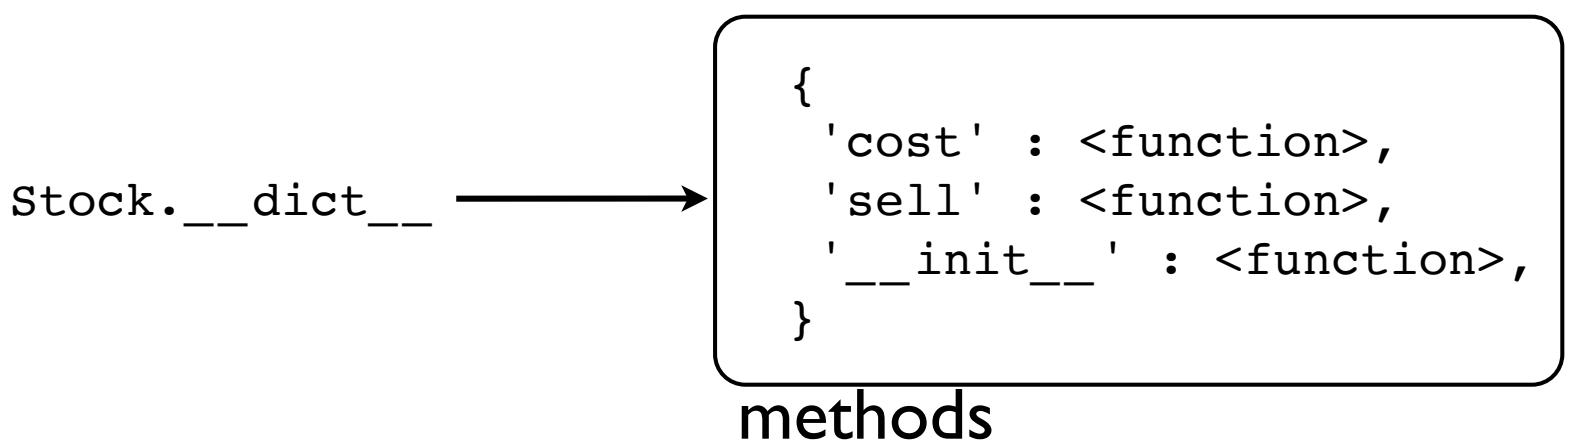
\includegraphics[keepaspectratio]{images/756c3a1f0b20e9bb25f8a201d5537c640990528144a7547d0694a79051052e4d.jpg}}

\bookmarksetup{startatroot}

\chapter{Instances and Classes}\label{instances-and-classes}

Instances and classes are linked together\\
\_ \_ class\_ \_ attribute refers back to the class

\begin{quote}
\begin{quote}
\begin{quote}
s \(\equiv\) Stock(`GOOG'，100，490.10)\\
s.\_dict\_\\
\{`name':`GOOG',`shares':100,`price':490.10\}\\
s.\_class\_\\
\textless class\_\_main\_\_.Stock'\textgreater{}
\end{quote}
\end{quote}
\end{quote}

The instance dictionary holds data unique to each instance whereas the
class dictionary holds data collectively shared by all instances

\bookmarksetup{startatroot}

\chapter{Instances and Classes}\label{instances-and-classes-1}

\pandocbounded{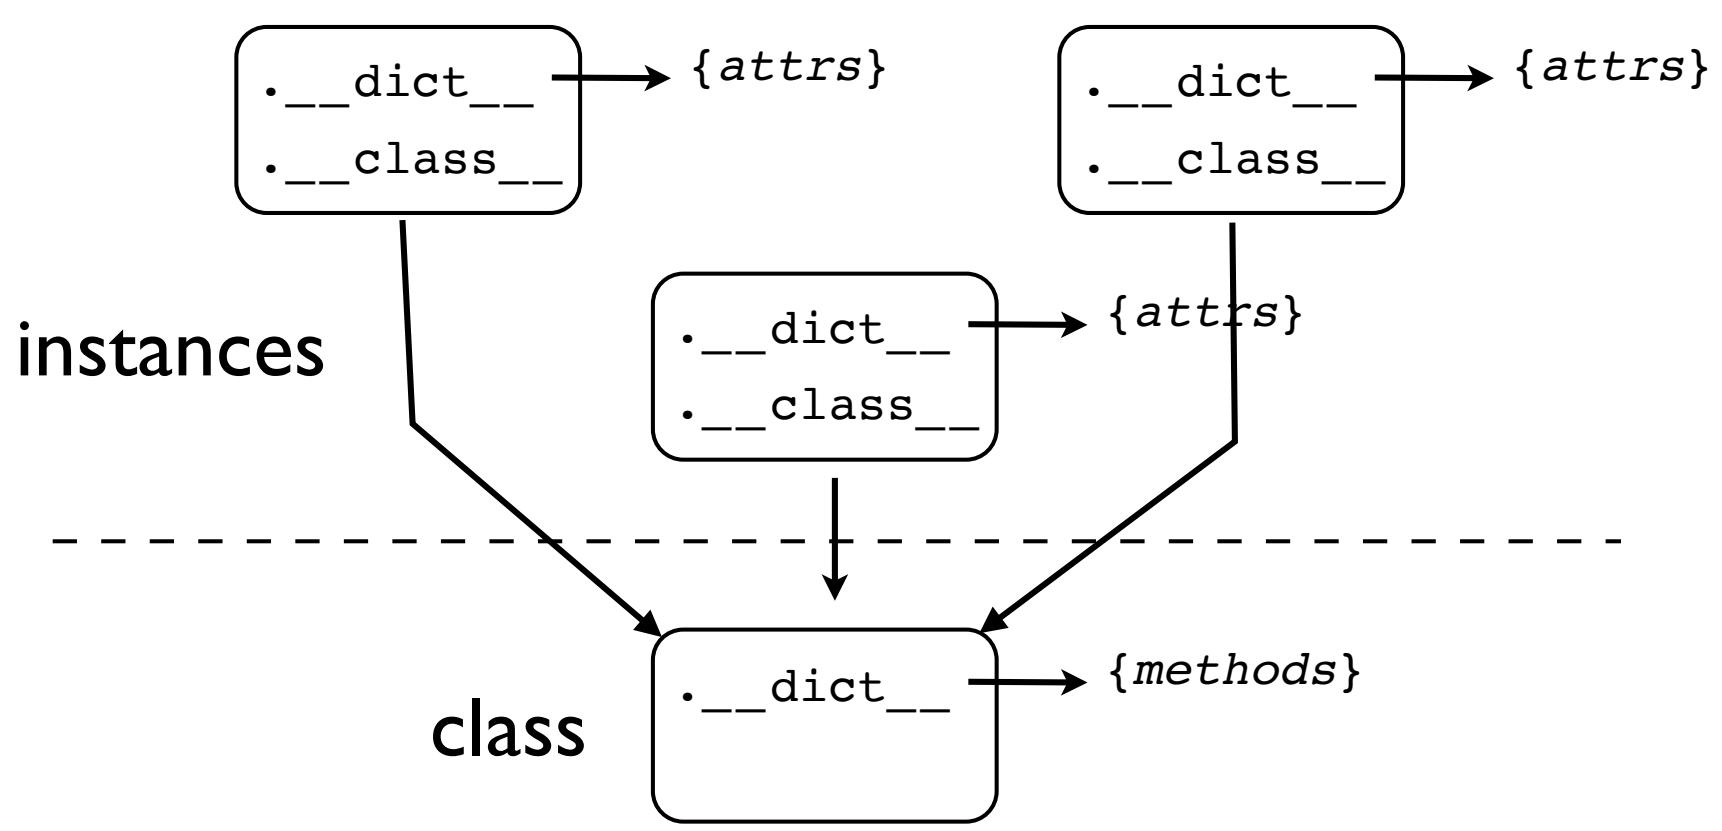
\includegraphics[keepaspectratio]{images/92487d542b64043d63800ff4ee426bd8b104508bc9cf6bfc012ca36accb73467.jpg}}

\bookmarksetup{startatroot}

\chapter{Attribute Access}\label{attribute-access}

• When you work with objects, you access data and methods using the (.)
operator

\begin{Shaded}
\begin{Highlighting}[]
\NormalTok{x = obj.name \#Getting obj.name = value \#Setting del obj.name \#Deleting }
\end{Highlighting}
\end{Shaded}

These operations are directly tied to the dictionaries sitting
underneath the covers

\bookmarksetup{startatroot}

\chapter{Modifying Instances}\label{modifying-instances}

Operations that modify an object always update the underlying dictionary

\begin{quote}
\begin{quote}
\begin{quote}
s \(\equiv\) Stock(`GOOG'，100,490.10)\\
s.\_\emph{dict}\\
\{`name':`GOOG'，`shares':100，`price':490.10\}
\end{quote}
\end{quote}
\end{quote}

\(\longrightarrow\) \textgreater\textgreater\textgreater{} s≧shares = 50

\begin{Shaded}
\begin{Highlighting}[]
\NormalTok{→ \textgreater{}\textgreater{}\textgreater{} s.date = \textquotesingle{}6/7/2007\textquotesingle{} }
\end{Highlighting}
\end{Shaded}

\begin{Shaded}
\begin{Highlighting}[]
\NormalTok{\textgreater{}\textgreater{}\textgreater{}s.\_\_dict\_}
\NormalTok{\{\textquotesingle{}name\textquotesingle{}:\textquotesingle{}GOOG\textquotesingle{},\textquotesingle{}shares\textquotesingle{}:50,\textquotesingle{}price\textquotesingle{}:490.10, \textquotesingle{}date\textquotesingle{}:\textquotesingle{}6/7/2007\textquotesingle{}\} }
\end{Highlighting}
\end{Shaded}

\(\longrightarrow\) \textgreater\textgreater\textgreater{} del s.share

\begin{Shaded}
\begin{Highlighting}[]
\NormalTok{\textgreater{}\textgreater{}\textgreater{}s.\_\_dict\_\_}
\NormalTok{\{\textquotesingle{}name\textquotesingle{}:\textquotesingle{}GOOG\textquotesingle{}, \textquotesingle{}price\textquotesingle{}:490.10, \textquotesingle{}date\textquotesingle{}:\textquotesingle{}6/7/2007\textquotesingle{}\}  }
\NormalTok{\textgreater{}\textgreater{}\textgreater{} }
\end{Highlighting}
\end{Shaded}

\bookmarksetup{startatroot}

\chapter{Reading Attributes}\label{reading-attributes}

• Suppose you read an attribute on an instance

\[
x = o b j. n a m e
\]

• Attribute may exist in two places

Local instance dictionary\\
Class dictionary

• So, both dictionaries may be checked

\bookmarksetup{startatroot}

\chapter{Reading Attributes}\label{reading-attributes-1}

First check in local \_ dict\_\\
If not found, look in \_ \_ dict\_ \_ of class

\pandocbounded{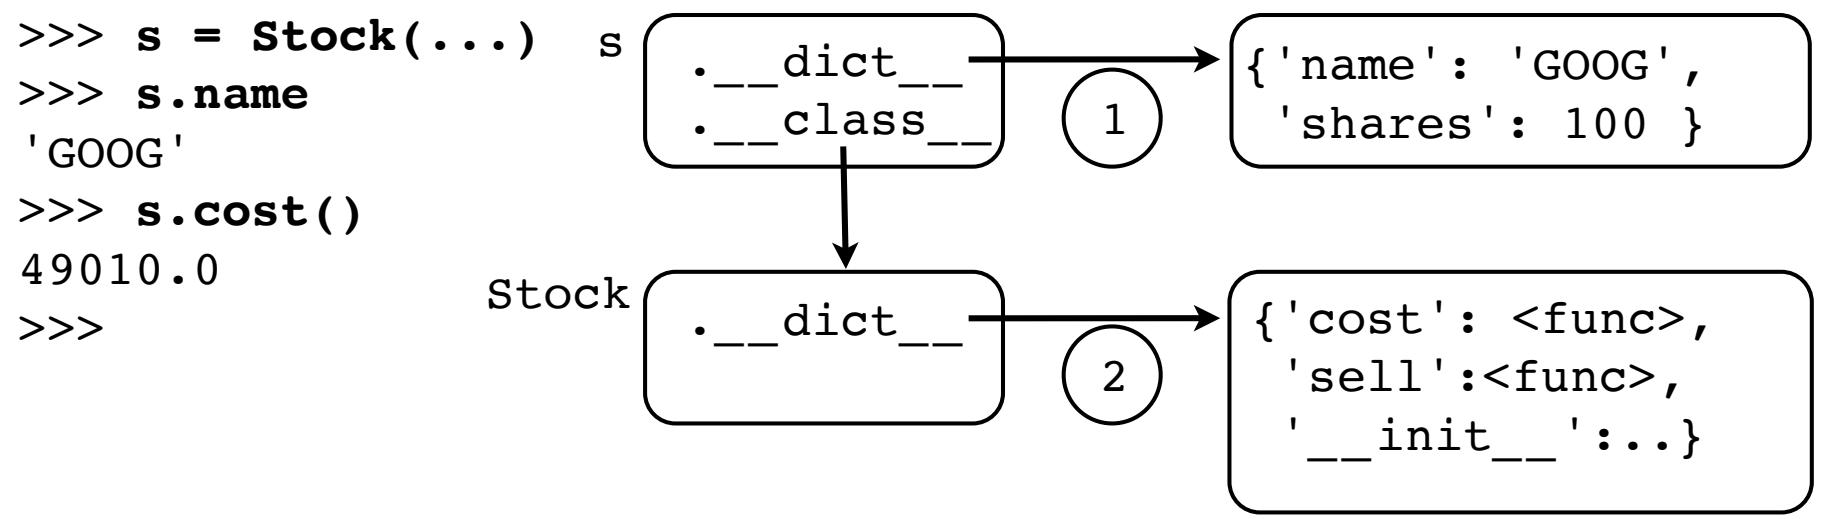
\includegraphics[keepaspectratio]{images/90934b195eb08c96187d92e149e16ef4e6c306ba56fe4a0ac1421609c97ad455.jpg}}

This lookup scheme is how the members of a class get shared by all
instances

\bookmarksetup{startatroot}

\chapter{Exercise 4.1}\label{exercise-4.1}

Time : 10 Minutes

\bookmarksetup{startatroot}

\chapter{How Inheritance Works}\label{how-inheritance-works}

• Classes may inherit from other classes class A(B,C): \ldots{}\\
Bases are stored as a tuple in each class
\textgreater\textgreater\textgreater{} A.\_\emph{bases} (\textless class
\_main\_\_.B'\textgreater,\textless class `\textbf{main}.C'\textgreater)
\textgreater\textgreater\textgreater{}\\
• This provides a link to parent classes\\
This link simply extends the search process used to find attributes

\bookmarksetup{startatroot}

\chapter{Reading Attributes}\label{reading-attributes-2}

First check in local \textbf{dict}\\
• If not found, look in \_ \_ dict\_ \_ of class\\
• If not found in class, look in base classes

\pandocbounded{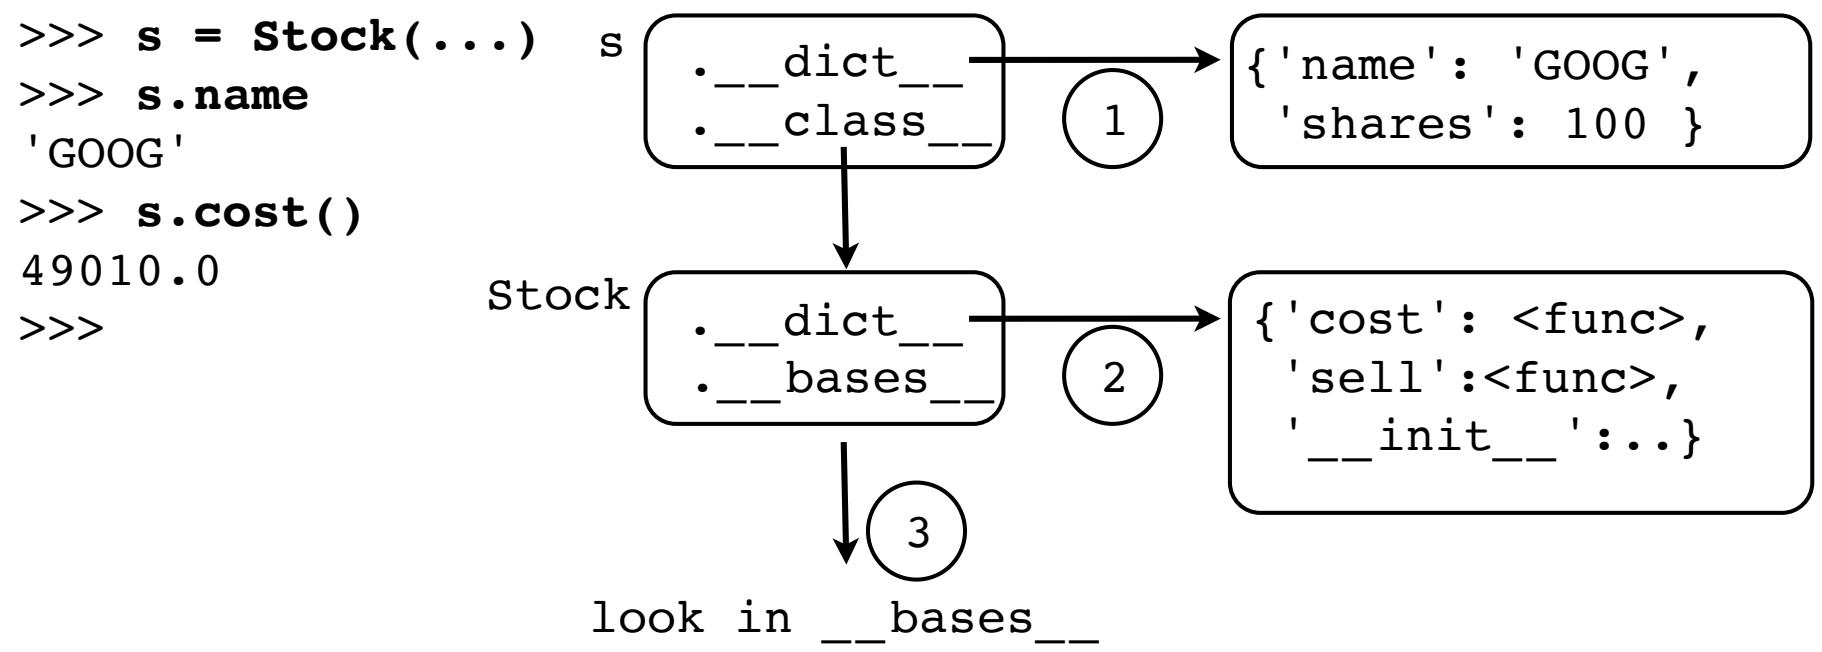
\includegraphics[keepaspectratio]{images/cc4181a664995506619c8a3ffb11f1415499f228bc0381999ecf3d1a8de1b5c9.jpg}}

\bookmarksetup{startatroot}

\chapter{Single Inheritance}\label{single-inheritance}

In inheritance hierarchies, attributes are found by walking up the
inheritance tree

class A(object): pass

class B(A): pass

class C(A): pass

class D(B): pass

class E(D): pass

With single inheritance, there is a single path to the top\\
• You stop with the first match

\pandocbounded{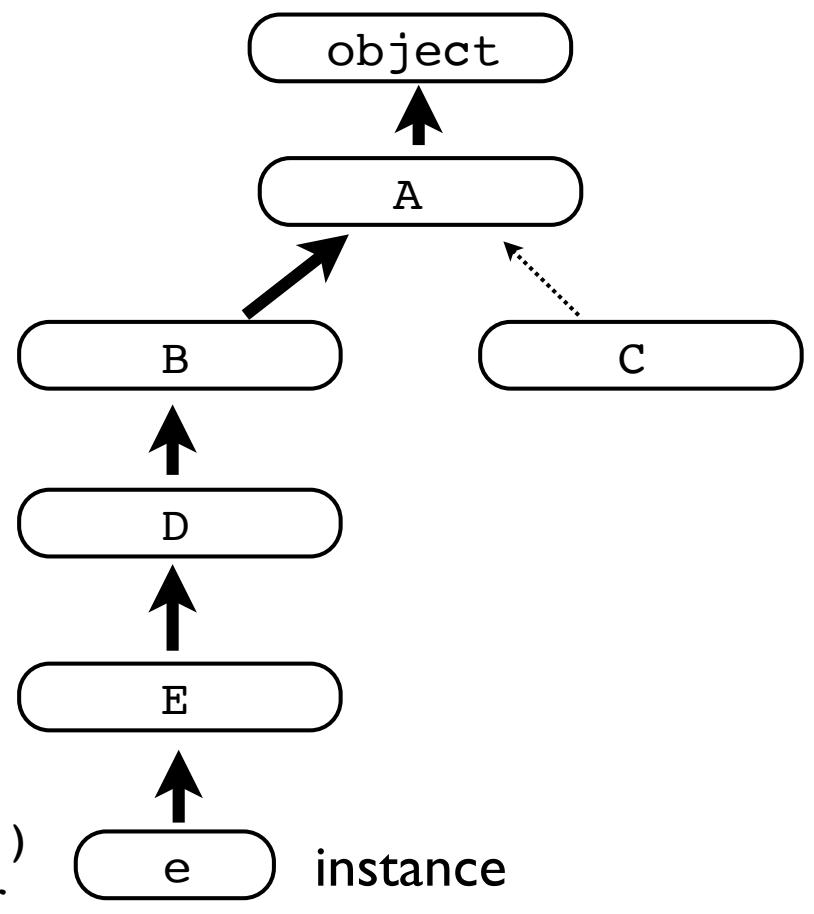
\includegraphics[keepaspectratio]{images/dbf570e5609fcb5fded49b1f08f58af62f8241b7594da1cd9edc079fccdc7e5a.jpg}}

e = E()

e.attr

\bookmarksetup{startatroot}

\chapter{The MRO}\label{the-mro}

The inheritance chain is precomputed and stored in an ``MRO'' attribute
on the class

\begin{Shaded}
\begin{Highlighting}[]
\NormalTok{\textgreater{}\textgreater{}\textgreater{} E.\_\_mro\_\_(\textless{}class\_\_main\_\_.E\textgreater{}， \textless{}class\_\_main\_\_.D\textgreater{}， \textless{}class\_\_main\_\_.B\textgreater{}， \textless{}class\_\_main\_\_.A\textgreater{}， \textless{}type \textquotesingle{}object\textquotesingle{}\textgreater{})   }
\NormalTok{\textgreater{}\textgreater{}\textgreater{}}
\end{Highlighting}
\end{Shaded}

``Method Resolution Order''\\
• To find attributes, Python walks the MRO\\
First match wins

\bookmarksetup{startatroot}

\chapter{Multiple Inheritance}\label{multiple-inheritance-2}

\bookmarksetup{startatroot}

\chapter{Consider this hierarchy}\label{consider-this-hierarchy}

class A(object): pass

class B(object): pass

class C(A,B): pass

class D(B): pass

class E(C,D): pass

\pandocbounded{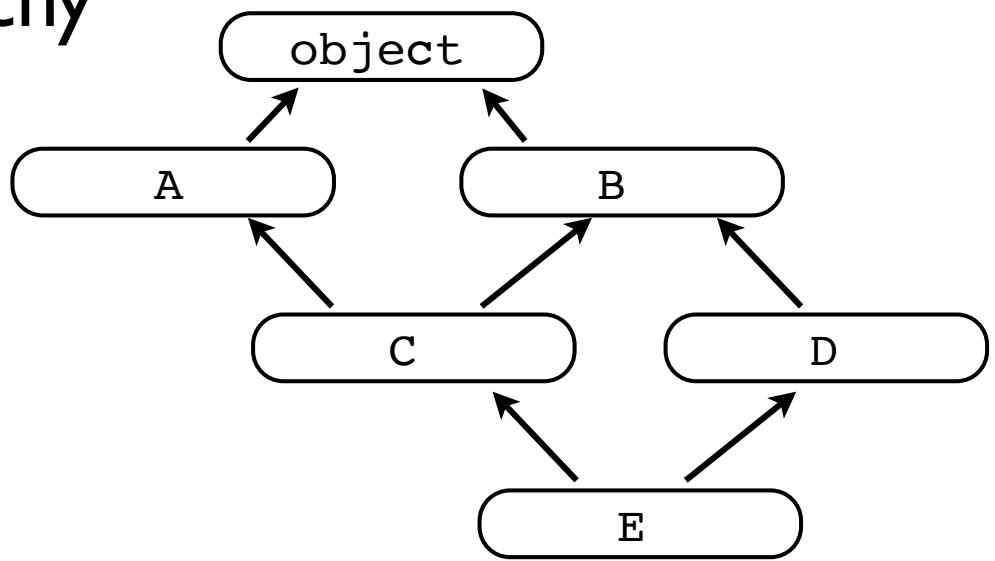
\includegraphics[keepaspectratio]{images/9951ff05fb5af54314431c756c33fe172d60cb900e1902b57b846c389a2b9147.jpg}}

\bookmarksetup{startatroot}

\chapter{What happens here?}\label{what-happens-here}

\[
\begin{array}{l} e = E (.) \\ e. a t t r \\ \end{array}
\]

\bookmarksetup{startatroot}

\chapter{• A similar search process is carried out, but there is an
added complication in that there may be many possible search
paths}\label{a-similar-search-process-is-carried-out-but-there-is-an-added-complication-in-that-there-may-be-many-possible-search-paths}

\bookmarksetup{startatroot}

\chapter{Multiple Inheritance}\label{multiple-inheritance-3}

Python uses ``cooperative multiple inheritance''\\
• There are some ordering rules:

Rule 1: Children before parents

Rule 2: Parents go in order

Inheritance works in two directions (up the hierarchy, across the list
of parents)

\pandocbounded{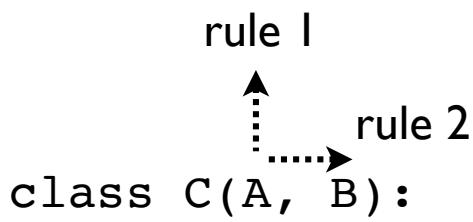
\includegraphics[keepaspectratio]{images/85463664ff118b5dee1b27349ef3a79b31b9564cc5d19ccd6f287c5a89c1c611.jpg}}

\bookmarksetup{startatroot}

\chapter{Multiple Inheritance}\label{multiple-inheritance-4}

• Multiple inheritance hierarchy is flattened

\begin{Shaded}
\begin{Highlighting}[]
\NormalTok{\textgreater{}\textgreater{}\textgreater{} E.\_\_mro\_\_(\textless{}class \textquotesingle{}main\textquotesingle{}.E\textgreater{}\textquotesingle{}》，\textless{}class \textquotesingle{}main.C\textquotesingle{}\textgreater{}，\textless{}class \textquotesingle{}main.A\textquotesingle{}\textgreater{}，\textless{}class \textquotesingle{}main.D\textquotesingle{}\textgreater{}，\textless{}class \textquotesingle{}main.B\textquotesingle{}\textgreater{}，\textless{}class \textquotesingle{}object\textquotesingle{}\textgreater{})  }
\NormalTok{\textgreater{}\textgreater{}\textgreater{} }
\end{Highlighting}
\end{Shaded}

Calculated using the C3 Linearization algorithm\\
• A constrained merge sort of parent MROs\\
An ordering based on ``the rules''\\
• Note: If you must know, there's also a third rule (first listed parent
wins if there's a ``tie'').

\bookmarksetup{startatroot}

\chapter{Multiple Inheritance}\label{multiple-inheritance-5}

• Consider classes with a common parent

class Base:

\pandocbounded{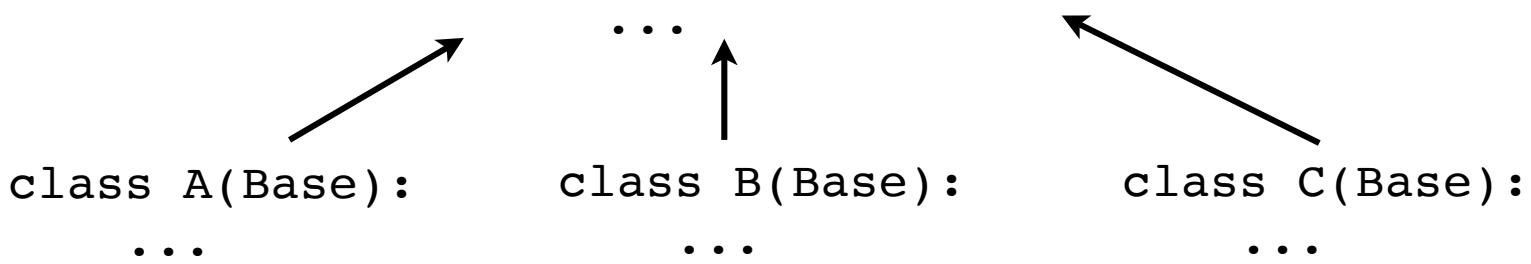
\includegraphics[keepaspectratio]{images/217336160f810c42f264add6dce5ba371d825a4a566aa63024f05e40726858fb.jpg}}

• All children of a common parent go first

class D(A,B,C):

\pandocbounded{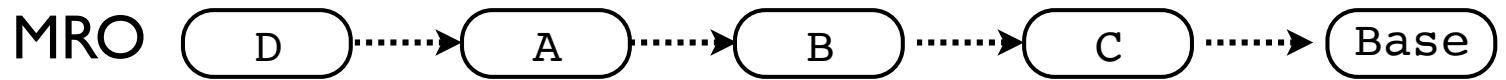
\includegraphics[keepaspectratio]{images/32ba28e4583c6e10a749c1417674de25f28da2cde6c033ad0836eafaf535308f.jpg}}

\bookmarksetup{startatroot}

\chapter{Why super()?}\label{why-super}

• Always use super() when overriding methods

class A(Base): def spam(self): return super().spam()

super() delegates to the next class on the MRO

\pandocbounded{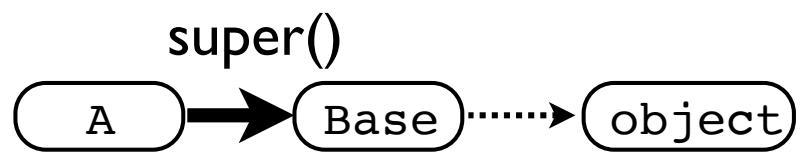
\includegraphics[keepaspectratio]{images/3742b6e0b859c4b1773941c14857a7c1d8a8c5e54497a21c58a204cb5d00a9ff.jpg}}

\pandocbounded{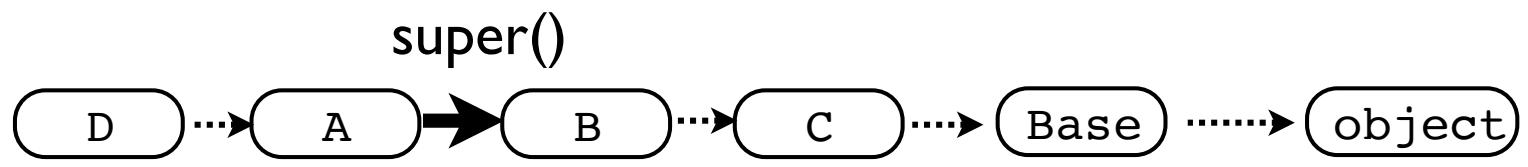
\includegraphics[keepaspectratio]{images/f58b16bcf4c0912664a0f3988d702cc255aa3357f09cfeac408f9294ea906285.jpg}}

• Tricky bit: You don't know what it is

\bookmarksetup{startatroot}

\chapter{super() Explained}\label{super-explained}

super() is one of the most poorly understood Python features

class A(Base):

def spam(self): vs.~Base.spam(self)

class A(Base):

def spam(self):

super().spam()

• These two classes are not the same\\
super() binds to the next implementation that is defined according to
the instance's MRO\\
• It's not necessarily the immediate parent

\bookmarksetup{startatroot}

\chapter{Designing for Inheritance}\label{designing-for-inheritance}

Rule 1: Compatible Method Arguments

\pandocbounded{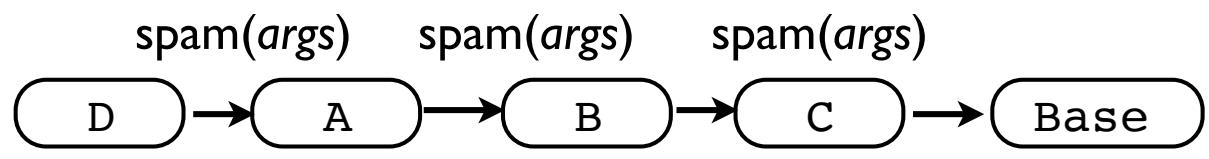
\includegraphics[keepaspectratio]{images/26daeeee40d355f493b8161fc1ff85a1cc52cd9048bbd1e234b2dc4cbe245f7a.jpg}}

Overridden methods must have a compatible signature across the entire
hierarchy\\
Remember: super() might not go to the immediate parent\\
Tip: If there are varying method signatures, use keyword arguments

\bookmarksetup{startatroot}

\chapter{Designing for Inheritance}\label{designing-for-inheritance-1}

Rule 2: Method chains must terminate

\pandocbounded{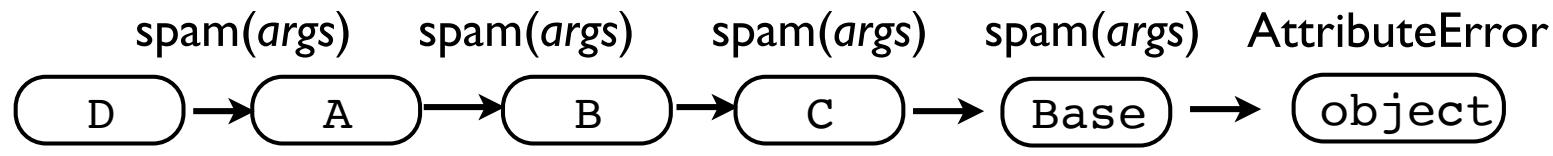
\includegraphics[keepaspectratio]{images/2ec4a0ab22e862a7c309aa45b0a6709c0e72e767320ebefbb00fc22a47850b0c.jpg}}

• You can't use super() forever--some class has to terminate the search
chain

class Base: def spam(self): pass

• Typically the role of an abstract base class

\bookmarksetup{startatroot}

\chapter{Designing for Inheritance}\label{designing-for-inheritance-2}

Rule 3: use super() everywhere

\pandocbounded{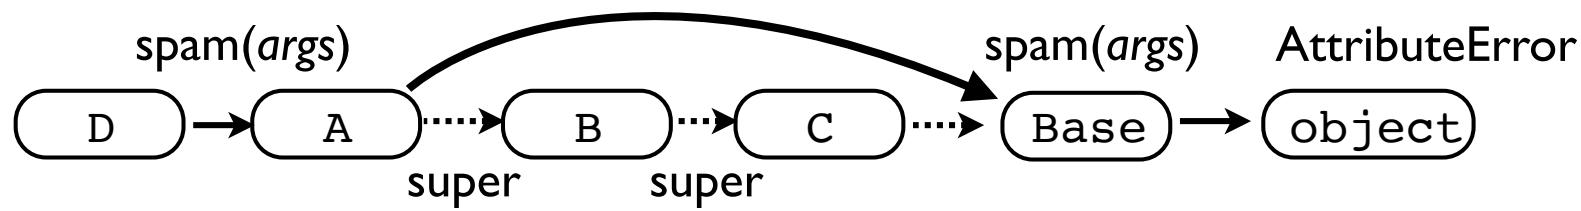
\includegraphics[keepaspectratio]{images/8164dfd3f57dfe67143f5c552b847e3e49f0f7ad0eef4dc63195077990123e1f.jpg}}

• Direct parent calls might explode heads

\begin{Shaded}
\begin{Highlighting}[]
\KeywordTok{class}\NormalTok{ A(Base):}
    \KeywordTok{def}\NormalTok{ spam(}\VariableTok{self}\NormalTok{):}
\NormalTok{        Base.spam(}\VariableTok{self}\NormalTok{)  }\CommentTok{\# NO! }
\end{Highlighting}
\end{Shaded}

If multiple inheritance is used, a direct parent call will probably
violate the MRO

\bookmarksetup{startatroot}

\chapter{Exercise 4.2}\label{exercise-4.2}

Time : 25 Minutes

\bookmarksetup{startatroot}

\chapter{Dicts and Classes (Reprise)}\label{dicts-and-classes-reprise}

\bookmarksetup{startatroot}

\chapter{Recall, a dictionary holds class
members}\label{recall-a-dictionary-holds-class-members}

class Stock: def \textbf{init}(self, name, shares, pr self.name = name
self.share = shares self.price = price def cost(self): return self.share
* self.price def sell(self, nshares): self.share \(= =\) nshares

\pandocbounded{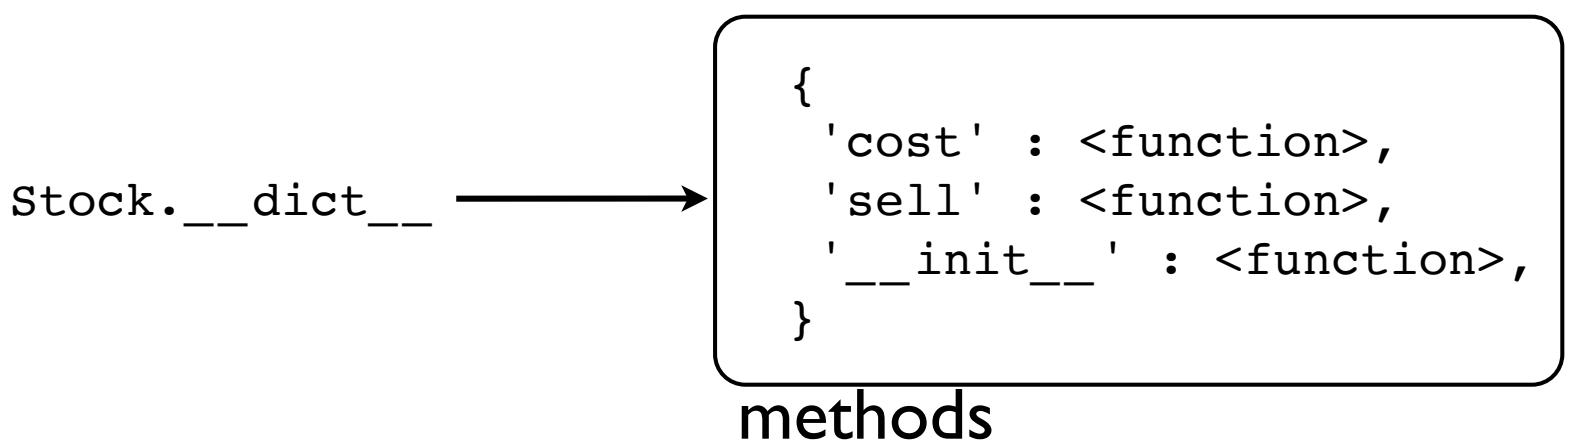
\includegraphics[keepaspectratio]{images/b9902283de55dbc04d3e11aa4f8395ec3e888ebe3b9eb6e2ec1e16a0e13efcf9.jpg}}

\bookmarksetup{startatroot}

\chapter{Reading Attributes (Reprise)}\label{reading-attributes-reprise}

Recall that a two-step process is used to locate attributes on objects

\pandocbounded{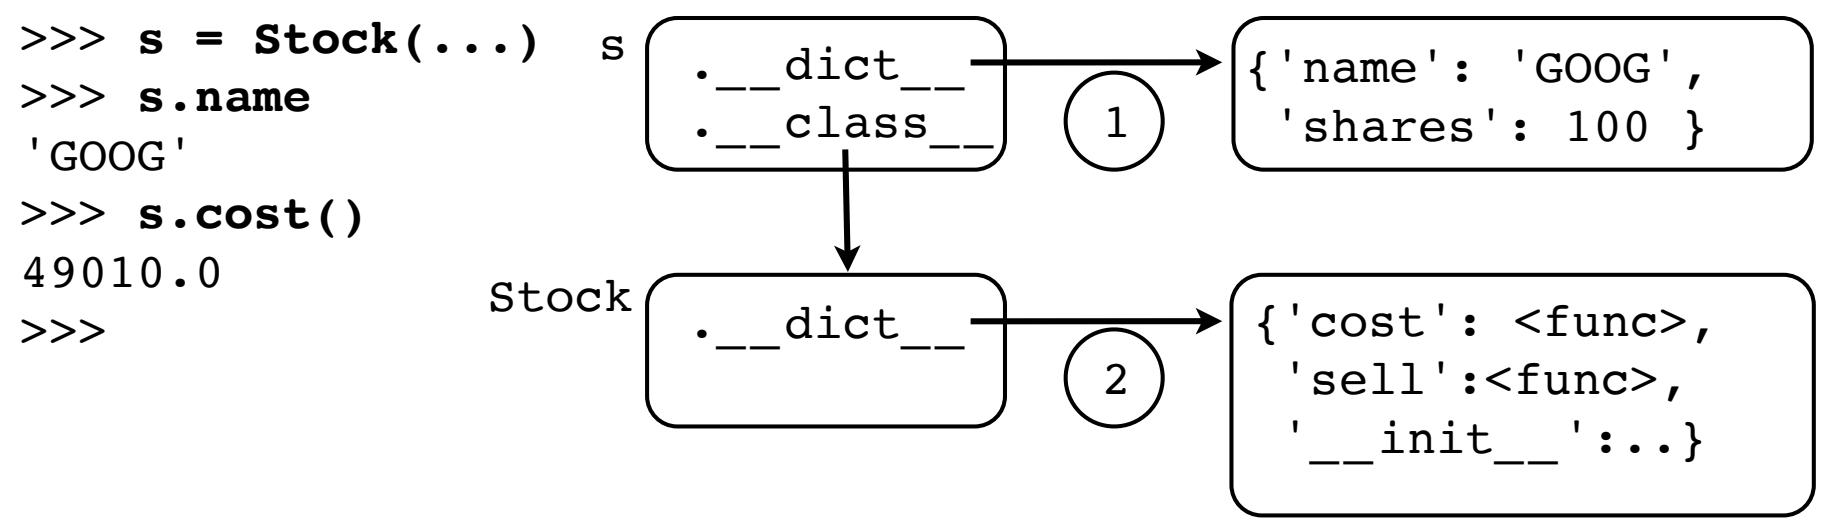
\includegraphics[keepaspectratio]{images/bc1942f2729b1cd0e66ffe2e84aebc6d927e7ab167b9ef4bbe3803e60f6015ef.jpg}}

This is mostly correct\\
• Except for the extra hidden magic (not shown)

\bookmarksetup{startatroot}

\chapter{Attribute Binding}\label{attribute-binding}

Access to attributes of classes involves one extra processing step\\
• Something known as the ``descriptor protocol''\\
It's so sneaky that most Python programmers don't even know it exists\\
• Yet, it holds the whole object system together

\bookmarksetup{startatroot}

\chapter{Descriptor Protocol}\label{descriptor-protocol}

Whenever an attribute is accessed on a class, the attribute is checked
to see if it is an object that looks like a so-called ``descriptor''\\
• A descriptor is an object with one or more of the following special
methods

d.\_\_get\_\_(obj, cls)\\
d.\_\_set\_\_(obj, value)\\
d.\_\_delete\_\_(obj)

If a descriptor is detected, one of the above methods gets triggered on
access

\bookmarksetup{startatroot}

\chapter{Descriptor Demo}\label{descriptor-demo}

Here is a class that implements a dummy descriptor (with prints for
debugging)

\begin{Shaded}
\begin{Highlighting}[]
\KeywordTok{class}\NormalTok{ Descriptor: }\KeywordTok{def} \FunctionTok{\_\_init\_\_}\NormalTok{(}\VariableTok{self}\NormalTok{, name): }\VariableTok{self}\NormalTok{.name }\OperatorTok{=}\NormalTok{ name }\KeywordTok{def} \FunctionTok{\_\_get\_\_}\NormalTok{(}\VariableTok{self}\NormalTok{, instance, cls): }\BuiltInTok{print}\NormalTok{(}\StringTok{\textquotesingle{}}\SpecialCharTok{\%s}\StringTok{:\_\_get\_\_\textquotesingle{}} \OperatorTok{\%} \VariableTok{self}\NormalTok{.name) }\KeywordTok{def} \FunctionTok{\_\_set\_\_}\NormalTok{(}\VariableTok{self}\NormalTok{, instance, value): }\BuiltInTok{print}\NormalTok{(}\StringTok{\textquotesingle{}}\SpecialCharTok{\%s}\StringTok{:\_\_set\_\_}\SpecialCharTok{\%s}\StringTok{\textquotesingle{}} \OperatorTok{\%}\NormalTok{ (}\VariableTok{self}\NormalTok{.name, value)) }\KeywordTok{def} \FunctionTok{\_\_delete\_\_}\NormalTok{(}\VariableTok{self}\NormalTok{, instance): }\BuiltInTok{print}\NormalTok{(}\StringTok{\textquotesingle{}}\SpecialCharTok{\%s}\StringTok{:\_\_delete\_\_\textquotesingle{}} \OperatorTok{\%} \VariableTok{self}\NormalTok{.name) }
\end{Highlighting}
\end{Shaded}

Basically, a descriptor is just an object with get, set, and delete
methods

\bookmarksetup{startatroot}

\chapter{Descriptor Demo}\label{descriptor-demo-1}

• Descriptors are placed in class definitions

class Foo:

a = Descriptor(`a')

b = Descriptor(`b')

• Now, watch what happens on access:

\begin{quote}
\begin{quote}
\begin{quote}
f = Foo()\\
f.a\\
a:\textbf{get}\\
f.a = 42\\
a:\textbf{set} 42\\
del f.a\\
a:\_\_delete\_\\
f.b\\
b:\textbf{get}
\end{quote}
\end{quote}
\end{quote}

\bookmarksetup{startatroot}

\chapter{Descriptor Demo}\label{descriptor-demo-2}

Descriptors are presented with information about the instance, class,
and values

\begin{Shaded}
\begin{Highlighting}[]
\KeywordTok{class}\NormalTok{ Descriptor: }\KeywordTok{def} \FunctionTok{\_\_init\_\_}\NormalTok{(}\VariableTok{self}\NormalTok{, name): f }\OperatorTok{=}\NormalTok{ Foo() }\VariableTok{self}\NormalTok{.name }\OperatorTok{=}\NormalTok{ name f.a }\KeywordTok{def} \FunctionTok{\_\_get\_\_}\NormalTok{(}\VariableTok{self}\NormalTok{, instance, cls): f.a }\OperatorTok{=} \DecValTok{42} \BuiltInTok{print}\NormalTok{(}\StringTok{\textquotesingle{}}\SpecialCharTok{\%s}\StringTok{:\_\_get\_\_\textquotesingle{}} \OperatorTok{\%} \VariableTok{self}\NormalTok{.name) }\KeywordTok{del}\NormalTok{ f.a }\KeywordTok{def} \FunctionTok{\_\_set\_\_}\NormalTok{(}\VariableTok{self}\NormalTok{, instance, value): }\BuiltInTok{print}\NormalTok{(}\StringTok{\textquotesingle{}}\SpecialCharTok{\%s}\StringTok{:\_\_set\_\_\textquotesingle{}} \OperatorTok{\%}\NormalTok{ (}\VariableTok{self}\NormalTok{.name, value)) }\KeywordTok{def} \FunctionTok{\_\_delete\_\_}\NormalTok{(}\VariableTok{self}\NormalTok{, instance): }\BuiltInTok{print}\NormalTok{(}\StringTok{\textquotesingle{}}\SpecialCharTok{\%s}\StringTok{:\_\_delete\_\_\textquotesingle{}} \OperatorTok{\%} \VariableTok{self}\NormalTok{.name) }
\end{Highlighting}
\end{Shaded}

Confusion: self is the descriptor itself, instance is the object it's
operating on.

\bookmarksetup{startatroot}

\chapter{Descriptor Storage}\label{descriptor-storage}

\bookmarksetup{startatroot}

\chapter{Descriptors store and retrieve
data}\label{descriptors-store-and-retrieve-data}

\begin{Shaded}
\begin{Highlighting}[]
\KeywordTok{class}\NormalTok{ Descriptor: }\KeywordTok{def} \FunctionTok{\_\_init\_\_}\NormalTok{(}\VariableTok{self}\NormalTok{, name): }\VariableTok{self}\NormalTok{.name }\OperatorTok{=}\NormalTok{ name }\KeywordTok{def} \FunctionTok{\_\_get\_\_}\NormalTok{(}\VariableTok{self}\NormalTok{, instance, cls}\OperatorTok{=}\VariableTok{None}\NormalTok{): }\ControlFlowTok{return}\NormalTok{ instance.\_\_dict\_\_(}\VariableTok{self}\NormalTok{.name) }\KeywordTok{def} \FunctionTok{\_\_set\_\_}\NormalTok{(}\VariableTok{self}\NormalTok{, instance, value): instance.\_\_dict\_\_(}\VariableTok{self}\NormalTok{.name] }\OperatorTok{=}\NormalTok{ value }
\end{Highlighting}
\end{Shaded}

\bookmarksetup{startatroot}

\chapter{Example:}\label{example-2}

\begin{Shaded}
\begin{Highlighting}[]
\KeywordTok{class}\NormalTok{ Foo(}\BuiltInTok{object}\NormalTok{):}
\NormalTok{    a }\OperatorTok{=}\NormalTok{ Descriptor(}\StringTok{\textquotesingle{}a\textquotesingle{}}\NormalTok{)}
\NormalTok{    b }\OperatorTok{=}\NormalTok{ Descriptor(}\StringTok{\textquotesingle{}b\textquotesingle{}}\NormalTok{) }
\end{Highlighting}
\end{Shaded}

Direct manipulation of the instance dictionary

\begin{Shaded}
\begin{Highlighting}[]
\NormalTok{f = Foo() }
\end{Highlighting}
\end{Shaded}

\begin{Shaded}
\begin{Highlighting}[]
\NormalTok{f.a }\OperatorTok{=} \DecValTok{23} \CommentTok{\# Stores value in f.\_\_dict\_\_[\textquotesingle{}a\textquotesingle{}] }
\end{Highlighting}
\end{Shaded}

\bookmarksetup{startatroot}

\chapter{Descriptor Binding}\label{descriptor-binding}

• Descriptors always override \_\_dict\_

\begin{Shaded}
\begin{Highlighting}[]
\KeywordTok{class}\NormalTok{ Foo:  }
\NormalTok{    a }\OperatorTok{=}\NormalTok{ Descriptor(}\StringTok{\textquotesingle{}a\textquotesingle{}}\NormalTok{)  }
\NormalTok{    b }\OperatorTok{=}\NormalTok{ Descriptor(}\StringTok{\textquotesingle{}b\textquotesingle{}}\NormalTok{) }
\end{Highlighting}
\end{Shaded}

• Modify the instance dict and try accessing

\begin{Shaded}
\begin{Highlighting}[]
\NormalTok{\textgreater{}\textgreater{}\textgreater{} f = Foo()}
\NormalTok{\textgreater{}\textgreater{}\textgreater{} f.\_\_dict\_\_[\textquotesingle{}a\textquotesingle{}] = 42}
\NormalTok{\textgreater{}\textgreater{}\textgreater{} f.\_\_dict\_\_}
\NormalTok{\{\textquotesingle{}a\textquotesingle{}: 42\}}
\NormalTok{\textgreater{}\textgreater{}\textgreater{} f.a}
\NormalTok{a:\_\_get\_\_}
\NormalTok{\textgreater{}\textgreater{}\textgreater{} notice how the descriptor runs regardless}
\NormalTok{the value in the instance dictionary }
\end{Highlighting}
\end{Shaded}

\bookmarksetup{startatroot}

\chapter{Who Cares?}\label{who-cares}

Every major feature of classes is implemented using descriptors

• Instance methods\\
Static methods ((\textbf{staticmethod?}))\\
• Class methods ((\textbf{classmethod?}))\\
Properties ((\textbf{property?}))\\
\emph{slots}

Descriptors provide the glue that connects instances and classes
together in the runtime

\bookmarksetup{startatroot}

\chapter{Descriptors in Action}\label{descriptors-in-action}

• Recall that . and () are separate operations

\begin{quote}
\begin{quote}
\begin{quote}
s = Stock(`GOOG',100,490.10)\\
s.cost\\
\textless body methodStock.cost of \(<  _{**}\) main\_.Stock object at
0x37e250\textgreater\textgreater{}\\
s.cost()\\
49010.0
\end{quote}
\end{quote}
\end{quote}

• Focus on that ``bound method'' result\\
• How did that get created? Magic?\\
No, a descriptor did that.

\bookmarksetup{startatroot}

\chapter{Descriptors in Action}\label{descriptors-in-action-1}

Behind the scenes of method lookup

\begin{Shaded}
\begin{Highlighting}[]
\NormalTok{\textgreater{}\textgreater{}\textgreater{} s = Stock(\textquotesingle{}GOOG\textquotesingle{}, 100, 490.10) }
\end{Highlighting}
\end{Shaded}

class attribute lookup \textgreater\textgreater\textgreater{} value
\(=\) Stock.\_dict\_{[}cost'{]}
\textgreater\textgreater\textgreater value \textless function cost at
0x378770\textgreater{}
\textgreater\textgreater\textgreater hasattr(value,``\textbf{get}'')\\
descripctor check and invocation True
\textgreater\textgreater\textgreater{} result \(=\)
value.\_get\_(s,Stock) \textgreater\textgreater\textgreater result
\textless bound method Stock.cost of \(<  _{ - }\) main\_.Stock object
at 0x37e250\textgreater\textgreater{}
\textgreater\textgreater\textgreater{} result() 49010.0

Functions are descriptors where \textbf{get}() creates the bound method
object

\bookmarksetup{startatroot}

\chapter{Descriptors and Properties}\label{descriptors-and-properties}

• Consider a class with a property attribute

\begin{Shaded}
\begin{Highlighting}[]
\KeywordTok{class}\NormalTok{ Stock: }\OperatorTok{@}\NormalTok{property }\KeywordTok{def}\NormalTok{ shares(}\VariableTok{self}\NormalTok{): }\ControlFlowTok{return} \VariableTok{self}\NormalTok{.\_shares }\OperatorTok{@}\NormalTok{shares setter }\KeywordTok{def}\NormalTok{ shares(}\VariableTok{self}\NormalTok{, value): }\VariableTok{self}\NormalTok{.\_shares }\OperatorTok{=}\NormalTok{ value }
\end{Highlighting}
\end{Shaded}

• A property is also a descriptor

\begin{quote}
\begin{quote}
\begin{quote}
s \(\equiv\) Stock()\\
p \(=\) Stock.\_\_dict\_\_{[}`shares'{]}\\
p\\
\textless property object at 0x3759c0\textgreater{}\\
p.\_set\_(s,100） \#Same as s.share \(= 100\)
\textgreater\textgreater\textgreater p.\_get\_(s,Stock)\#Same as
s.share\\
100\\
s.share\\
100
\end{quote}
\end{quote}
\end{quote}

\bookmarksetup{startatroot}

\chapter{Descriptors and slots}\label{descriptors-and-slots}

Consider a class with slots

class Foo:

\[
\_ \text {s l o t s} _ {- - } = \left(^ {\prime} x ^ {\prime}, ^ {\prime} y ^ {\prime}, ^ {\prime} z ^ {\prime}\right)
\]

\[
\begin{array}{c c c} \bullet & \bullet & \bullet \end{array}
\]

Internally, an array is allocated

0 1 2

x

y

z

Each slot name is used to create a descriptor that simply gets or sets
values in the appropriate array position (internals are implemented in C
and hard to view though)

\bookmarksetup{startatroot}

\chapter{Descriptor Commentary}\label{descriptor-commentary}

Descriptors are one of Python's most powerful customizations (you own
the dot)\\
Experts can create their own custom descriptors and use them to change
what happens in the low levels of the object system\\
• Often used in advanced programming frameworks and as an encapsulation
tool

\bookmarksetup{startatroot}

\chapter{Descriptor Application}\label{descriptor-application}

A common use of descriptors is in describing data (e.g., Object
Relational Mapping, etc.)

\begin{Shaded}
\begin{Highlighting}[]
\KeywordTok{class}\NormalTok{ Stock:  }
\NormalTok{    name }\OperatorTok{=}\NormalTok{ String(}\StringTok{\textquotesingle{}name\textquotesingle{}}\NormalTok{, maxlen}\OperatorTok{=}\DecValTok{8}\NormalTok{)  }
\NormalTok{    shares }\OperatorTok{=}\NormalTok{ Integer(}\StringTok{\textquotesingle{}shares\textquotesingle{}}\NormalTok{)  }
\NormalTok{    price }\OperatorTok{=}\NormalTok{ Real(}\StringTok{\textquotesingle{}price\textquotesingle{}}\NormalTok{) }
\end{Highlighting}
\end{Shaded}

• Provide more precise control than properties.\\
Results in less repetitive code

\bookmarksetup{startatroot}

\chapter{Descriptor Application}\label{descriptor-application-1}

\bookmarksetup{startatroot}

\chapter{Example descriptor code:}\label{example-descriptor-code}

\begin{Shaded}
\begin{Highlighting}[]
\KeywordTok{class}\NormalTok{ Integer: }\KeywordTok{def} \FunctionTok{\_\_init\_\_}\NormalTok{(}\VariableTok{self}\NormalTok{, name): }\VariableTok{self}\NormalTok{.name }\OperatorTok{=}\NormalTok{ name }\KeywordTok{def} \FunctionTok{\_\_get\_\_}\NormalTok{(}\VariableTok{self}\NormalTok{, instance, cls): }\ControlFlowTok{return}\NormalTok{ instance.\_\_dict\_\_(}\VariableTok{self}\NormalTok{.name] }\KeywordTok{def} \FunctionTok{\_\_set\_\_}\NormalTok{(}\VariableTok{self}\NormalTok{, instance, value): }\ControlFlowTok{if} \KeywordTok{not} \BuiltInTok{isinstance}\NormalTok{(value, }\BuiltInTok{int}\NormalTok{): }\ControlFlowTok{raise} \PreprocessorTok{TypeError}\NormalTok{(}\StringTok{\textquotesingle{}Expected an integer\textquotesingle{}}\NormalTok{) instance.\_\_dict\_\_(}\VariableTok{self}\NormalTok{.name] }\OperatorTok{=}\NormalTok{ value }
\end{Highlighting}
\end{Shaded}

\bookmarksetup{startatroot}

\chapter{\texorpdfstring{Minor note: \textbf{get}() can be omitted if
the name exactly matches that in the instance
dict}{Minor note: get() can be omitted if the name exactly matches that in the instance dict}}\label{minor-note-get-can-be-omitted-if-the-name-exactly-matches-that-in-the-instance-dict}

\bookmarksetup{startatroot}

\chapter{Tricky Bits with get}\label{tricky-bits-with-get}

\textbf{get} can be accessed in two ways class Foo: a = Descriptor(`a')

Through an instance (bound)

\[
\begin{array}{l} \text {f = F O O ()} \\ \text {f . a} \end{array}
\]

• On the class definition itself (unbound) Foo.a\\
Example : Instance vs.~class methods

\bookmarksetup{startatroot}

\chapter{Tricky Bits with get}\label{tricky-bits-with-get-1}

Recommended \textbf{get} implementation

\begin{Shaded}
\begin{Highlighting}[]
\KeywordTok{class}\NormalTok{ Descriptor: }\KeywordTok{def} \FunctionTok{\_\_get\_\_}\NormalTok{(}\VariableTok{self}\NormalTok{, instance, cls): }\ControlFlowTok{if}\NormalTok{ instance }\KeywordTok{is} \VariableTok{None}\NormalTok{: }\CommentTok{\# If no instance given, return the descriptor \# object itself return self else: \# Return the instance value return instance.\_\_dict\_\_(self.name] }
\end{Highlighting}
\end{Shaded}

• Always check for presence of an instance (instance). If None, return
the descriptor itself

\bookmarksetup{startatroot}

\chapter{Method Descriptors}\label{method-descriptors}

• A weaker descriptor that only has \textbf{get}\\
class MethodDescriptor: def \textbf{get}(self, instance, cls):
print(`Getting!')\\
• Only triggered if obj.\_\_dict\_\_ doesn't match

\begin{Shaded}
\begin{Highlighting}[]
\KeywordTok{class}\NormalTok{ Foo(}\BuiltInTok{object}\NormalTok{):}
\NormalTok{    a }\OperatorTok{=}\NormalTok{ MethodDescriptor(}\StringTok{"a"}\NormalTok{)}
\OperatorTok{\textgreater{}\textgreater{}\textgreater{}}\NormalTok{ f }\OperatorTok{=}\NormalTok{ Foo()}
\OperatorTok{\textgreater{}\textgreater{}\textgreater{}}\NormalTok{ f.a}
\NormalTok{Getting}\OperatorTok{!}
\OperatorTok{\textgreater{}\textgreater{}\textgreater{}}\NormalTok{ f.\_\_dict\_\_[}\StringTok{\textquotesingle{}a\textquotesingle{}}\NormalTok{] }\OperatorTok{=} \DecValTok{42}
\OperatorTok{\textgreater{}\textgreater{}\textgreater{}}\NormalTok{ f.a}
\DecValTok{42}
\OperatorTok{\textgreater{}\textgreater{}\textgreater{}}\NormalTok{ Notice how the value }\KeywordTok{in}\NormalTok{ the dictionary hides the descriptor }
\end{Highlighting}
\end{Shaded}

\bookmarksetup{startatroot}

\chapter{Descriptor Naming}\label{descriptor-naming}

\bookmarksetup{startatroot}

\chapter{• Descriptors can define a name
setter}\label{descriptors-can-define-a-name-setter}

\begin{Shaded}
\begin{Highlighting}[]
\KeywordTok{class}\NormalTok{ Descriptor: }\KeywordTok{def} \FunctionTok{\_\_init\_\_}\NormalTok{(}\VariableTok{self}\NormalTok{, name}\OperatorTok{=}\VariableTok{None}\NormalTok{): }\VariableTok{self}\NormalTok{.name }\OperatorTok{=}\NormalTok{ name }\KeywordTok{def} \FunctionTok{\_\_get\_\_}\NormalTok{(}\VariableTok{self}\NormalTok{, instance, cls): }\ControlFlowTok{return}\NormalTok{ instance.\_\_dict\_\_(}\VariableTok{self}\NormalTok{.name) }\KeywordTok{def} \FunctionTok{\_\_set\_name\_\_}\NormalTok{(}\VariableTok{self}\NormalTok{, cls, name): }\VariableTok{self}\NormalTok{.name }\OperatorTok{=}\NormalTok{ name }
\end{Highlighting}
\end{Shaded}

\bookmarksetup{startatroot}

\chapter{Gets information about definition
context}\label{gets-information-about-definition-context}

\begin{Shaded}
\begin{Highlighting}[]
\KeywordTok{class}\NormalTok{ Spam(}\BuiltInTok{object}\NormalTok{):}
\NormalTok{    x }\OperatorTok{=}\NormalTok{ Descriptor()}
\NormalTok{        x.\_set\_name\_\_(Spam, }\StringTok{\textquotesingle{}x\textquotesingle{}}\NormalTok{) }
\end{Highlighting}
\end{Shaded}

\bookmarksetup{startatroot}

\chapter{Python 3.6+ only}\label{python-3.6-only}

\bookmarksetup{startatroot}

\chapter{Descriptor Conflicts}\label{descriptor-conflicts}

• Multiple descriptors per attribute aren't allowed

\begin{Shaded}
\begin{Highlighting}[]
\KeywordTok{class}\NormalTok{ Point: \_sLOTS\_ }\OperatorTok{=}\NormalTok{ (}\StringTok{\textquotesingle{}x\textquotesingle{}}\NormalTok{, }\StringTok{\textquotesingle{}y\textquotesingle{}}\NormalTok{) x }\OperatorTok{=}\NormalTok{ Integer() y }\OperatorTok{=}\NormalTok{ Integer() }
\end{Highlighting}
\end{Shaded}

\begin{Shaded}
\begin{Highlighting}[]
\NormalTok{Traceback (most recent call last):}
\NormalTok{    File "\textless{}stdin\textgreater{}", line 1, in \textless{}module\textgreater{}}
\NormalTok{ValueError: \textquotesingle{}x\textquotesingle{} in \_\_slots\_\_ conflicts with class variable }
\end{Highlighting}
\end{Shaded}

• There can only one descriptor in charge\\
• Coordination is possible (but tricky)

\bookmarksetup{startatroot}

\chapter{Exercise 4.3}\label{exercise-4.3}

Time : 15 Minutes

\bookmarksetup{startatroot}

\chapter{Attribute Access Methods}\label{attribute-access-methods}

Classes can intercept attribute access\\
Set of special methods for setting, deleting, and getting attributes

\pandocbounded{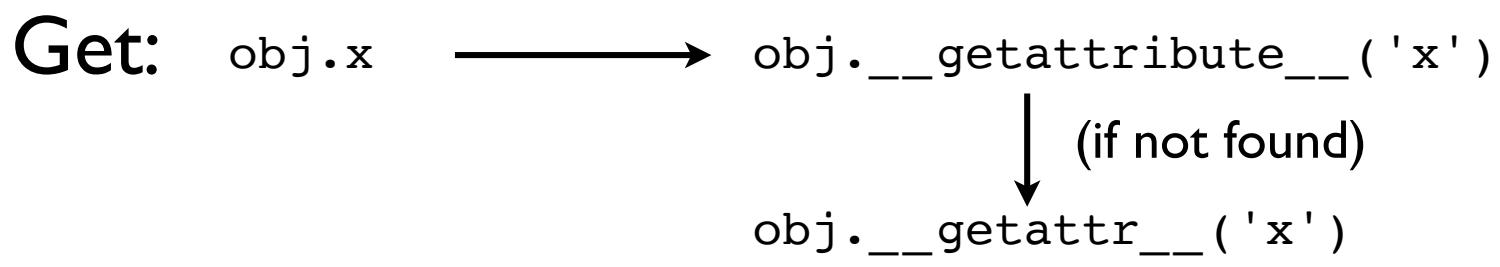
\includegraphics[keepaspectratio]{images/b93402a514bb106889276e2485ad9858c8b289693fb599230bfaa1b1c7fa2ad0.jpg}}

\pandocbounded{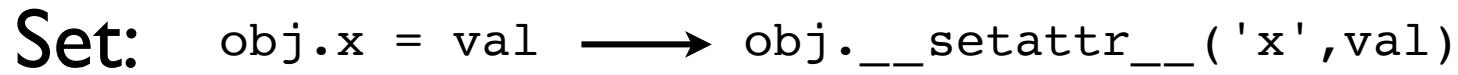
\includegraphics[keepaspectratio]{images/2747b26bad3b66e6ec482a7c0793d47ca3e8c57d35554e1953d3a67c19c493e5.jpg}}

\pandocbounded{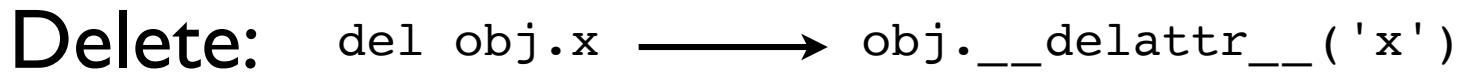
\includegraphics[keepaspectratio]{images/a596fae17e6b6c7c7c091a8aad1cd99c49a90f4f40a9cfe3c7b135517a5e5ce3.jpg}}

\bookmarksetup{startatroot}

\chapter{\_getattribute ()}\label{getattribute}

\textbf{getattribute}(self,name)\\
• Called every time an attribute is read\\
Default behavior looks for descriptors, checks the instance dictionary,
checks bases classes (inheritance), etc.\\
If it can't find the attribute after all of those steps, it invokes \_
\_ getattr\_ \_ (self,name)

\bookmarksetup{startatroot}

\chapter{\_\_getattr () method}\label{getattr-method}

\textbf{getattr}(self,name)\\
• A failsafe method. Called if an attribute can't be found using the
standard mechanism\\
• Default behavior is to raise AttributeError\\
Sometimes customized

\bookmarksetup{startatroot}

\chapter{setattr () method}\label{setattr-method}

\_ setattr\_ \_ (self,name,value)\\
• Called every time an attribute is set\\
Default behavior checks for descriptors, stores values in the instance
dictionary, etc.

\bookmarksetup{startatroot}

\chapter{delattr () method}\label{delattr-method}

delattr\_ \_ (self,name)\\
• Called every time an attribute is deleted\\
Default behavior checks for descriptors and deletes from the instance
dictionary

\bookmarksetup{startatroot}

\chapter{Customizing Access}\label{customizing-access}

A class can redefine the attribute access methods to implement custom
processing\\
The most common application of this is for creating wrapper objects,
proxies, and other similar kinds of objects

\bookmarksetup{startatroot}

\chapter{Example : Proxy}\label{example-proxy}

\bookmarksetup{startatroot}

\chapter{Consider this class}\label{consider-this-class}

\begin{Shaded}
\begin{Highlighting}[]
\KeywordTok{class}\NormalTok{ Proxy: }\KeywordTok{def} \FunctionTok{\_\_init\_\_}\NormalTok{(}\VariableTok{self}\NormalTok{,obj): }\VariableTok{self}\NormalTok{.\_obj }\OperatorTok{=}\NormalTok{ obj }\KeywordTok{def} \FunctionTok{\_\_getattr\_\_}\NormalTok{(}\VariableTok{self}\NormalTok{,name): }\BuiltInTok{print}\NormalTok{(}\StringTok{\textquotesingle{}getattr:\textquotesingle{}}\NormalTok{，name) }\ControlFlowTok{return} \BuiltInTok{getattr}\NormalTok{(}\VariableTok{self}\NormalTok{.\_obj，name) }
\end{Highlighting}
\end{Shaded}

• It holds an internal reference to an object\\
• Attribute access is redirected to held object

\bookmarksetup{startatroot}

\chapter{Example : Proxy}\label{example-proxy-1}

\bookmarksetup{startatroot}

\chapter{• Example use:}\label{example-use-3}

\begin{Shaded}
\begin{Highlighting}[]
\NormalTok{\textgreater{}\textgreater{}\textgreater{} c = Circle(4.0)  }
\NormalTok{\textgreater{}\textgreater{}\textgreater{} c.radius  }
\NormalTok{4.0  }
\NormalTok{\textgreater{}\textgreater{}\textgreater{} c.area()  }
\NormalTok{50.26548245743669  }
\NormalTok{\textgreater{}\textgreater{}\textgreater{} p = Proxy(c)  }
\NormalTok{\textgreater{}\textgreater{}\textgreater{} p  }
\NormalTok{\textless{}\_\_main\_\_.Proxy object at 0x37f130\textgreater{}  }
\NormalTok{\textgreater{}\textgreater{}\textgreater{} p radius  }
\NormalTok{getattr: radius  }
\NormalTok{4.0  }
\NormalTok{\textgreater{}\textgreater{}\textgreater{} p.area()  }
\NormalTok{gets captured by \_\_getattr\_\_  }
\NormalTok{getattr: area  }
\NormalTok{50.26548245743669  }
\NormalTok{\textgreater{}\textgreater{}\textgreater{} notice how attribute access gets captured by \_\_getattr\_\_ and then redirected to the original object }
\end{Highlighting}
\end{Shaded}

\bookmarksetup{startatroot}

\chapter{Example: Delegation}\label{example-delegation}

class A:

\begin{Shaded}
\begin{Highlighting}[]
\KeywordTok{def}\NormalTok{ foo(}\VariableTok{self}\NormalTok{):}
    \BuiltInTok{print}\NormalTok{(}\StringTok{\textquotesingle{}A.foo\textquotesingle{}}\NormalTok{)}
\KeywordTok{def}\NormalTok{ bar(}\VariableTok{self}\NormalTok{):}
    \BuiltInTok{print}\NormalTok{(}\StringTok{\textquotesingle{}A.bar\textquotesingle{}}\NormalTok{) }
\end{Highlighting}
\end{Shaded}

class B:

\begin{Shaded}
\begin{Highlighting}[]
\KeywordTok{def} \FunctionTok{\_\_init\_\_}\NormalTok{(}\VariableTok{self}\NormalTok{):}
    \VariableTok{self}\NormalTok{.\_a }\OperatorTok{=}\NormalTok{ A()}
\KeywordTok{def}\NormalTok{ bar(}\VariableTok{self}\NormalTok{):}
    \BuiltInTok{print}\NormalTok{(}\StringTok{\textquotesingle{}B.bar\textquotesingle{}}\NormalTok{)}
    \VariableTok{self}\NormalTok{.\_a.bar()}
\KeywordTok{def} \FunctionTok{\_\_getattr\_\_}\NormalTok{(}\VariableTok{self}\NormalTok{, name):}
    \ControlFlowTok{return} \BuiltInTok{getattr}\NormalTok{(}\VariableTok{self}\NormalTok{.\_a, name) }
\end{Highlighting}
\end{Shaded}

Example:

\begin{Shaded}
\begin{Highlighting}[]
\NormalTok{\textgreater{}\textgreater{}\textgreater{} b = B()  }
\NormalTok{\textgreater{}\textgreater{}\textgreater{} b.foo()  }
\NormalTok{A.foo  }
\NormalTok{\textgreater{}\textgreater{}\textgreater{} b.bar()  }
\NormalTok{B.bar  }
\NormalTok{A.bar  }
\NormalTok{\textgreater{}\textgreater{}\textgreater{} }
\end{Highlighting}
\end{Shaded}

• Sometimes used as an alternative to inheritance

\bookmarksetup{startatroot}

\chapter{Delegation Caution}\label{delegation-caution}

\textbf{getattr} doesn't apply to special methods (e.g., \textbf{len},
\textbf{getitem}, etc.)\\
• Must delegate manually (if needed)

class B:

def init\_\_(self): self.\_a = A()

def \textbf{getitem}(self, index): return self.\_a{[}index{]}

def \textbf{getattr}(self, name): return getattr(self.\_a, name)

\bookmarksetup{startatroot}

\chapter{Exercise 4.4}\label{exercise-4.4}

Time : 10 Minutes

\bookmarksetup{startatroot}

\chapter{Section 5}\label{section-5}

\bookmarksetup{startatroot}

\chapter{Functions}\label{functions}

\bookmarksetup{startatroot}

\chapter{Overview}\label{overview-2}

Function design\\
• Functional Programming\\
Error handling and Logging\\
Testing

\bookmarksetup{startatroot}

\chapter{Functions}\label{functions-1}

Functions are a basic building block\\
− Top-level functions in a module\\
• Methods of a class\\
• Almost all of your code should live in a function

\bookmarksetup{startatroot}

\chapter{Function Design}\label{function-design}

• Try to make functions ``self-contained''

arguments

\pandocbounded{
\includegraphics[keepaspectratio]{images/ca3c2511c58421678ff66a7382fd40c25fc3abd27f5105004349989844f02435.jpg}}

function

\pandocbounded{
\includegraphics[keepaspectratio]{images/8762a47c27006b51709d3e43419e90fe5ff3b3ffe1853f808bfe5399b59c1b4a.jpg}}

result

• Only operate on passed arguments\\
• Produce the same result for same arguments\\
• Avoid hidden side-effects\\
Goals: Simplicity and Predictability

\bookmarksetup{startatroot}

\chapter{Function Invocation}\label{function-invocation}

• Names and arguments are the ``interface''

\begin{Shaded}
\begin{Highlighting}[]
\NormalTok{result = some\_func(args) }
\end{Highlighting}
\end{Shaded}

\pandocbounded{
\includegraphics[keepaspectratio]{images/ab5e51b0f49d592f303fc46b0dd3c4a5614c76e797f85fe8e32ae669ec83388e.jpg}}

• Calling a function should be intuitive and easy\\
• It's a core component of making an API

\bookmarksetup{startatroot}

\chapter{Naming Conventions}\label{naming-conventions-1}

• There is a preferred Python ``style''\\
• Functions should use lowercase names and

def read\_data(filename): •

def readData(filename): ..

Yes

No

• Use a leading \_ for internal/private funcs

def \_internal\_func():

\bookmarksetup{startatroot}

\chapter{Default Arguments}\label{default-arguments}

• Sometimes you want default arguments

def read\_data(filename, debug=False):

If an argument value is assigned, the argument is optional in function
calls

\[
\begin{array}{l} d = \text {r e a d} _ {\text {d a t a}} \left(^ {\prime} \text {d a t a . c s v} ^ {\prime}\right) \\ e = \text {r e a d} _ {\text {d a t a}} \left(^ {\prime} \text {d a t a . c s v} ^ {\prime}, \text {d e b u g} = \text {T r u e}\right) \\ \end{array}
\]

• Default arguments must appear last in definition

\bookmarksetup{startatroot}

\chapter{Keyword Arguments}\label{keyword-arguments}

• Prefer keywords for passing optional arguments

a = read\_data(`data.csv', debug \(=\) True) \# YES!

b = read\_data(`data.csv', True) \# NO!

Keywords result in better code clarity\\
• You can force the use of keyword arguments

def read\_data(filename, *, debug=False):

All arguments after the * must be given as by keyword

\bookmarksetup{startatroot}

\chapter{Default Values}\label{default-values}

• Don't use mutable values as defaults

\begin{Shaded}
\begin{Highlighting}[]
\KeywordTok{def}\NormalTok{ func(a, items }\OperatorTok{=}\NormalTok{ [ ]):}
\NormalTok{    items.append(a)}
    \ControlFlowTok{return}\NormalTok{ items }
\end{Highlighting}
\end{Shaded}

The default value is only created once for the whole program--mutations
are ``sticky''

\begin{Shaded}
\begin{Highlighting}[]
\OperatorTok{\textgreater{}\textgreater{}\textgreater{}} \FunctionTok{func(}\DecValTok{1}\FunctionTok{)}  
\FunctionTok{[}\DecValTok{1}\FunctionTok{]}  
\OperatorTok{\textgreater{}\textgreater{}\textgreater{}} \FunctionTok{func(}\DecValTok{2}\FunctionTok{)}  
\FunctionTok{[}\DecValTok{1}\FunctionTok{,} \DecValTok{2}\FunctionTok{]}  
\OperatorTok{\textgreater{}\textgreater{}\textgreater{}} \FunctionTok{func(}\DecValTok{3}\FunctionTok{)}  
\FunctionTok{[}\DecValTok{1}\FunctionTok{,} \DecValTok{2}\FunctionTok{,} \DecValTok{3}\FunctionTok{]} 
\end{Highlighting}
\end{Shaded}

\bookmarksetup{startatroot}

\chapter{Default Values}\label{default-values-1}

Advice: Only use immutable values such as None, True, False, numbers, or
strings

\begin{Shaded}
\begin{Highlighting}[]
\KeywordTok{def}\NormalTok{ func(a, items}\OperatorTok{=}\VariableTok{None}\NormalTok{): }\ControlFlowTok{if}\NormalTok{ items }\KeywordTok{is} \VariableTok{None}\NormalTok{: items }\OperatorTok{=}\NormalTok{ [] items.append(a) }\ControlFlowTok{return}\NormalTok{ items }
\end{Highlighting}
\end{Shaded}

This avoids the problem of the default being modified by accident

\begin{Shaded}
\begin{Highlighting}[]
\NormalTok{\textgreater{}\textgreater{}\textgreater{} func(1)  }
\NormalTok{[1]  }
\NormalTok{\textgreater{}\textgreater{}\textgreater{} func(2)  }
\NormalTok{[2]  }
\NormalTok{\textgreater{}\textgreater{}\textgreater{} }
\end{Highlighting}
\end{Shaded}

\bookmarksetup{startatroot}

\chapter{Optional Values}\label{optional-values}

• Sometimes you need to express optional values\\
• Most common convention is to use None

name \(=\) None \# Not assigned name \(=\) `Guido' \# Assigned

• Test against None when you use it

if name is not None: print(`Hello', name)

• Caution: Often error-prone if not careful

\bookmarksetup{startatroot}

\chapter{Argument Transformation}\label{argument-transformation}

\bookmarksetup{startatroot}

\chapter{Consider}\label{consider}

def read\_data(filename): records \(=\) {[}{]} with open(filename) as f:
for line in f: records.append(record) return records Compare with def
read\_data lines): records \(= [ ]\) for line in lines:
records.append(record) return records

\bookmarksetup{startatroot}

\chapter{Argument Transforms}\label{argument-transforms}

• This version is far more flexible

def read\_data lines): records \(= \left[\right]\) for line in lines:
records.append(record) return records

\begin{Shaded}
\begin{Highlighting}[]
\ControlFlowTok{with} \BuiltInTok{open}\NormalTok{(}\StringTok{\textquotesingle{}Data.csv\textquotesingle{}}\NormalTok{) }\ImportTok{as}\NormalTok{ f: data }\OperatorTok{=}\NormalTok{ read\_data(f)   }
\ControlFlowTok{with}\NormalTok{ gzip.}\BuiltInTok{open}\NormalTok{(}\StringTok{\textquotesingle{}Data.csv.gz\textquotesingle{}}\NormalTok{, }\StringTok{\textquotesingle{}rt\textquotesingle{}}\NormalTok{) }\ImportTok{as}\NormalTok{ f: data }\OperatorTok{=}\NormalTok{ read\_data(f)   }
\NormalTok{r }\OperatorTok{=}\NormalTok{ requests.get(}\StringTok{\textquotesingle{}http://place/data.csv\textquotesingle{}}\NormalTok{)   }
\NormalTok{data }\OperatorTok{=}\NormalTok{ read\_data(r.iteratorlinesdecode\_unICODE}\OperatorTok{=}\StringTok{\textquotesingle{}utf{-}8\textquotesingle{}}\NormalTok{)) }
\end{Highlighting}
\end{Shaded}

• Question: Should you embrace flexibility?

\bookmarksetup{startatroot}

\chapter{Doc Strings}\label{doc-strings}

• Functions should have a doc string

\begin{Shaded}
\begin{Highlighting}[]
\KeywordTok{def}\NormalTok{ add(x, y):}
\NormalTok{    ...}
\NormalTok{    Adds x }\KeywordTok{and}\NormalTok{ y together.}
\NormalTok{    ...}
    \ControlFlowTok{return}\NormalTok{ x }\OperatorTok{+}\NormalTok{ y }
\end{Highlighting}
\end{Shaded}

• Feeds the help() command and development tools

\bookmarksetup{startatroot}

\chapter{Type Hints (PEP 484)}\label{type-hints-pep-484}

• Optional annotations can indicate types

\begin{Shaded}
\begin{Highlighting}[]
\KeywordTok{def}\NormalTok{ add(x:}\BuiltInTok{int}\NormalTok{, y:}\BuiltInTok{int}\NormalTok{) }\OperatorTok{{-}\textgreater{}} \BuiltInTok{int}\NormalTok{:}
\NormalTok{    ...}
\NormalTok{    Adds x }\KeywordTok{and}\NormalTok{ y together.}
\NormalTok{    ...}
    \ControlFlowTok{return}\NormalTok{ x }\OperatorTok{+}\NormalTok{ y }
\end{Highlighting}
\end{Shaded}

The type hints do nothing, but may be useful for code checkers,
documentation, IDEs, etc.

\begin{Shaded}
\begin{Highlighting}[]
\NormalTok{\textgreater{}\textgreater{}\textgreater{} help (add)  }
\NormalTok{Help on function add in module \_\_main\_\_:  }
\NormalTok{add(x:int, y:int) {-}\textgreater{} int  }
\NormalTok{Adds x and y }
\end{Highlighting}
\end{Shaded}

\bookmarksetup{startatroot}

\chapter{Commentary on Type Hints}\label{commentary-on-type-hints}

On the whole, it is probably a good idea to add type-hints to your code
if it makes code easier for others to understand. However, if your goal
is to automatically type-check Python with the rigor of a compiled
language (e.g., C++, Java, etc.) you need to be aware that type hints
have been retrofitted on Python as a late addition to the language and
that this has introduced a wide variety of very complex issues beyond
the scope of this course. Moreover, there are many classic Python
programming idioms that are notoriously difficult to accurately ``type''
in straightforward way. Yes, you could spend a lot of time trying to
make the type-checker happy. Or, not. Personally, I tend to take a
pragmatic approach to types. If I'm writing new code, I'll try to make
it type-friendly. However, if the complexity starts to spiral out of
control, I'm more inclined to rethink my approach as opposed to playing
some kind of whack-a-mole game with the type checker. Your mileage might
vary. -- Dave

\bookmarksetup{startatroot}

\chapter{Exercise 5.1}\label{exercise-5.1}

Time : 10 Minutes

\bookmarksetup{startatroot}

\chapter{Function Results}\label{function-results}

• Have the function cleanly return a result

function

\pandocbounded{
\includegraphics[keepaspectratio]{images/79ad978e524cd040df536d854dcd678ac52cfaa8e53213054a31004a502498b0.jpg}}

result

• Return multiple values with a tuple if needed

\begin{Shaded}
\begin{Highlighting}[]
\KeywordTok{def}\NormalTok{ divide(x, y):}
\NormalTok{    quotient }\OperatorTok{=}\NormalTok{ x }\OperatorTok{//}\NormalTok{ y}
\NormalTok{    remainder }\OperatorTok{=}\NormalTok{ x }\OperatorTok{\%}\NormalTok{ y}
    \ControlFlowTok{return}\NormalTok{ (quotient, remainder) }
\end{Highlighting}
\end{Shaded}

\bookmarksetup{startatroot}

\chapter{Returning Optionals}\label{returning-optionals}

• Sometimes a function returns an ``optional'' value\\
• Common convention is to return None\\
Example: Pattern Matching (re module)

\begin{Shaded}
\begin{Highlighting}[]
\NormalTok{\textgreater{}\textgreater{}\textgreater{} import re   }
\NormalTok{\textgreater{}\textgreater{}\textgreater{} m = re.match(\textquotesingle{}\textbackslash{}\textbackslash{}d\textquotesingle{}+,\textquotesingle{}abc\textquotesingle{})   }
\NormalTok{\textgreater{}\textgreater{}\textgreater{} print(m)   }
\NormalTok{None   }
\NormalTok{\textgreater{}\textgreater{}\textgreater{} m = re.match(\textquotesingle{}\textbackslash{}\textbackslash{}d\textquotesingle{}+,\textquotesingle{}123\textquotesingle{})   }
\NormalTok{\textgreater{}\textgreater{}\textgreater{} print(m)   }
\NormalTok{\textless{}\_sre.SRE\_Match object; span=(0, 3), match=\textquotesingle{}123\textquotesingle{}\textgreater{}   }
\NormalTok{\textgreater{}\textgreater{}\textgreater{} }
\end{Highlighting}
\end{Shaded}

• For errors: raise an exception instead

\bookmarksetup{startatroot}

\chapter{Concurrency}\label{concurrency}

• Functions might execute concurrently (threads)

\begin{Shaded}
\begin{Highlighting}[]
\KeywordTok{def}\NormalTok{ foo():}
\NormalTok{    ...}
\KeywordTok{def}\NormalTok{ bar():}
\NormalTok{    ...}
\ImportTok{from}\NormalTok{ threading }\ImportTok{import}\NormalTok{ Thread}
\NormalTok{t1 }\OperatorTok{=}\NormalTok{ Thread(target}\OperatorTok{=}\NormalTok{foo)}
\NormalTok{t1.start()}
\NormalTok{t2 }\OperatorTok{=}\NormalTok{ thread(target}\OperatorTok{=}\NormalTok{bar)}
\NormalTok{t2.start() }
\end{Highlighting}
\end{Shaded}

\pandocbounded{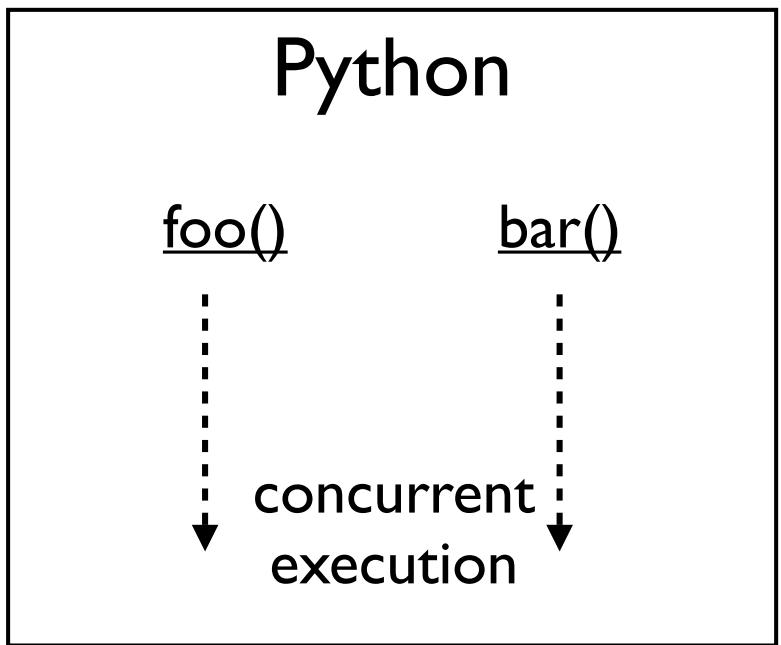
\includegraphics[keepaspectratio]{images/bce01377239aa4e57917b26d8fed6060e628321242e73b986c1f8047f02d7c54.jpg}}

• Shared state, execution in single interpreter

\bookmarksetup{startatroot}

\chapter{Futures}\label{futures}

Represents a future result (to be computed)

from concurrent.futures import Future

fut \(=\) Future()

To store a result

fut.set\_result(value)

To wait for a result

value \(=\) fut.result()

Coordination is required

\bookmarksetup{startatroot}

\chapter{Future Example}\label{future-example}

def func(x, y, fut):

time.sleep(20)

fut.set\_result(x+y)

def caller():

fut \(=\) Future()

threading.Thread(target \(=\) func, args=(2, 3, fut)).start()

result \(=\) fut.result()

print(`Got:', result)

• Reminder: Concurrent execution of both functions\\
This underlying pattern is used in many contexts (threads, async,
multiprocessing, etc.)

\bookmarksetup{startatroot}

\chapter{Exercise 5.2}\label{exercise-5.2}

Time : 15 Minutes

\bookmarksetup{startatroot}

\chapter{Functional Programming}\label{functional-programming}

• Programming style characterized by

Functions\\
No sides effects/mutability\\
Higher order functions

\bookmarksetup{startatroot}

\chapter{Higher Order Functions}\label{higher-order-functions}

Essential features\ldots{}

Functions can accept functions as input\\
Functions can return functions as results

Python supports both

\bookmarksetup{startatroot}

\chapter{Functions as Input}\label{functions-as-input}

\bookmarksetup{startatroot}

\chapter{• Consider these two
functions}\label{consider-these-two-functions}

\begin{Shaded}
\begin{Highlighting}[]
\KeywordTok{def}\NormalTok{ sum\_squares(nums):}
\NormalTok{    total }\OperatorTok{=} \DecValTok{0}
    \ControlFlowTok{for}\NormalTok{ n }\KeywordTok{in}\NormalTok{ nums:}
\NormalTok{        total }\OperatorTok{+=}\NormalTok{ n }\OperatorTok{*}\NormalTok{ n}
    \ControlFlowTok{return}\NormalTok{ total}
\KeywordTok{def}\NormalTok{ sum\_cubes(nums):}
\NormalTok{    total }\OperatorTok{=} \DecValTok{0}
    \ControlFlowTok{for}\NormalTok{ n }\KeywordTok{in}\NormalTok{ nums:}
\NormalTok{        total }\OperatorTok{+=}\NormalTok{ n }\OperatorTok{**} \DecValTok{3}
    \ControlFlowTok{return}\NormalTok{ total }
\end{Highlighting}
\end{Shaded}

\bookmarksetup{startatroot}

\chapter{They're almost identical (one line
differs)}\label{theyre-almost-identical-one-line-differs}

\bookmarksetup{startatroot}

\chapter{Functions as Input}\label{functions-as-input-1}

• Recognizing commonality is part of abstraction

def sum\_map(func, nums): total = 0 for n in nums: total += func(n)
return total def square(x): return x * x\\
nums \(= [1\) ,2,3,4{]}\\
r = sum\_map(square, nums)

• This version allows any function to be passed\\
• Sometimes referred to as a ``callback function''

\bookmarksetup{startatroot}

\chapter{Lambda Functions}\label{lambda-functions}

• One-expression functions can use lambda

\begin{Shaded}
\begin{Highlighting}[]
\KeywordTok{def}\NormalTok{ sum\_map(func, nums): total }\OperatorTok{=} \DecValTok{0} \ControlFlowTok{for}\NormalTok{ n }\KeywordTok{in}\NormalTok{ nums: total }\OperatorTok{+=}\NormalTok{ func(n) }\ControlFlowTok{return}\NormalTok{ total }
\end{Highlighting}
\end{Shaded}

\(\mathbf{nums} = [1,2,3,4]\) result \(=\) sum\_map( lambda
\(\mathbf{x}\) : \(\mathbf{x}^{*}\mathbf{x}\) ,nums)

Creates an anonymous function (on the spot)\\
• Can only contain a single expression\\
• No control flow, exceptions, etc.

\bookmarksetup{startatroot}

\chapter{Partial Application}\label{partial-application}

• Lambda often used to alter function args

\begin{Shaded}
\begin{Highlighting}[]
\NormalTok{def distance(x, y): return abs(x {-} y) }
\end{Highlighting}
\end{Shaded}

\begin{Shaded}
\begin{Highlighting}[]
\OperatorTok{\textgreater{}\textgreater{}\textgreater{}} \FunctionTok{distance(}\DecValTok{10}\FunctionTok{,} \DecValTok{20}\FunctionTok{)}  
\DecValTok{10}  
\OperatorTok{\textgreater{}\textgreater{}\textgreater{}} \CharTok{dist\_from10} \OperatorTok{=} \CharTok{lambda} \CharTok{y}\FunctionTok{:} \FunctionTok{distance(}\DecValTok{10}\FunctionTok{,} \CharTok{y}\FunctionTok{)}  
\OperatorTok{\textgreater{}\textgreater{}\textgreater{}} \FunctionTok{dist\_from10(}\DecValTok{3}\FunctionTok{)}  
\DecValTok{7}  
\OperatorTok{\textgreater{}\textgreater{}\textgreater{}} \FunctionTok{dist\_from10(}\DecValTok{14}\FunctionTok{)}  
\DecValTok{4}  
\OperatorTok{\textgreater{}\textgreater{}\textgreater{}} 
\end{Highlighting}
\end{Shaded}

functools.partial

\begin{Shaded}
\begin{Highlighting}[]
\ImportTok{from}\NormalTok{ functools }\ImportTok{import}\NormalTok{ partial dist\_from10 }\OperatorTok{=}\NormalTok{ partial(distance, }\DecValTok{10}\NormalTok{) }
\end{Highlighting}
\end{Shaded}

\bookmarksetup{startatroot}

\chapter{Map-Reduce}\label{map-reduce}

• You can sometimes decompose the code further

\begin{Shaded}
\begin{Highlighting}[]
\NormalTok{def sum\_map(func, nums): total = 0 for n in nums: func(n) Mapping total += func(n) return total + = Reduction  }
\NormalTok{nums = [1, 2, 3, 4] r = sum\_map(lambda x: x*x, nums) }
\end{Highlighting}
\end{Shaded}

• There are two basic operations (+, func)

\bookmarksetup{startatroot}

\chapter{Map-Reduce}\label{map-reduce-1}

\begin{Shaded}
\begin{Highlighting}[]
\KeywordTok{def} \BuiltInTok{map}\NormalTok{(func, values): result }\OperatorTok{=}\NormalTok{ [] }\ControlFlowTok{for}\NormalTok{ x }\KeywordTok{in}\NormalTok{ values: result.append(func(x)) }\ControlFlowTok{return}\NormalTok{ result }
\end{Highlighting}
\end{Shaded}

\begin{Shaded}
\begin{Highlighting}[]
\KeywordTok{def} \BuiltInTok{reduce}\NormalTok{(func, values, initial}\OperatorTok{=}\DecValTok{0}\NormalTok{):}
\NormalTok{    result }\OperatorTok{=}\NormalTok{ initial}
    \ControlFlowTok{for}\NormalTok{ n }\KeywordTok{in}\NormalTok{ values:}
\NormalTok{        result }\OperatorTok{=}\NormalTok{ func(n, result)}
    \ControlFlowTok{return}\NormalTok{ result }
\end{Highlighting}
\end{Shaded}

\begin{Shaded}
\begin{Highlighting}[]
\NormalTok{def sum(x, y): return x + y }
\end{Highlighting}
\end{Shaded}

\begin{Shaded}
\begin{Highlighting}[]
\KeywordTok{def}\NormalTok{ square(x): }\ControlFlowTok{return}\NormalTok{ x }\OperatorTok{*}\NormalTok{ x }
\end{Highlighting}
\end{Shaded}

\(\mathrm{nums} = [1,2,3,4]\) result \(=\)
reduce(sum，map(square，nums))

\bookmarksetup{startatroot}

\chapter{Commentary}\label{commentary-3}

Subdividing problems into small composable parts is a useful software
architecture tool

\pandocbounded{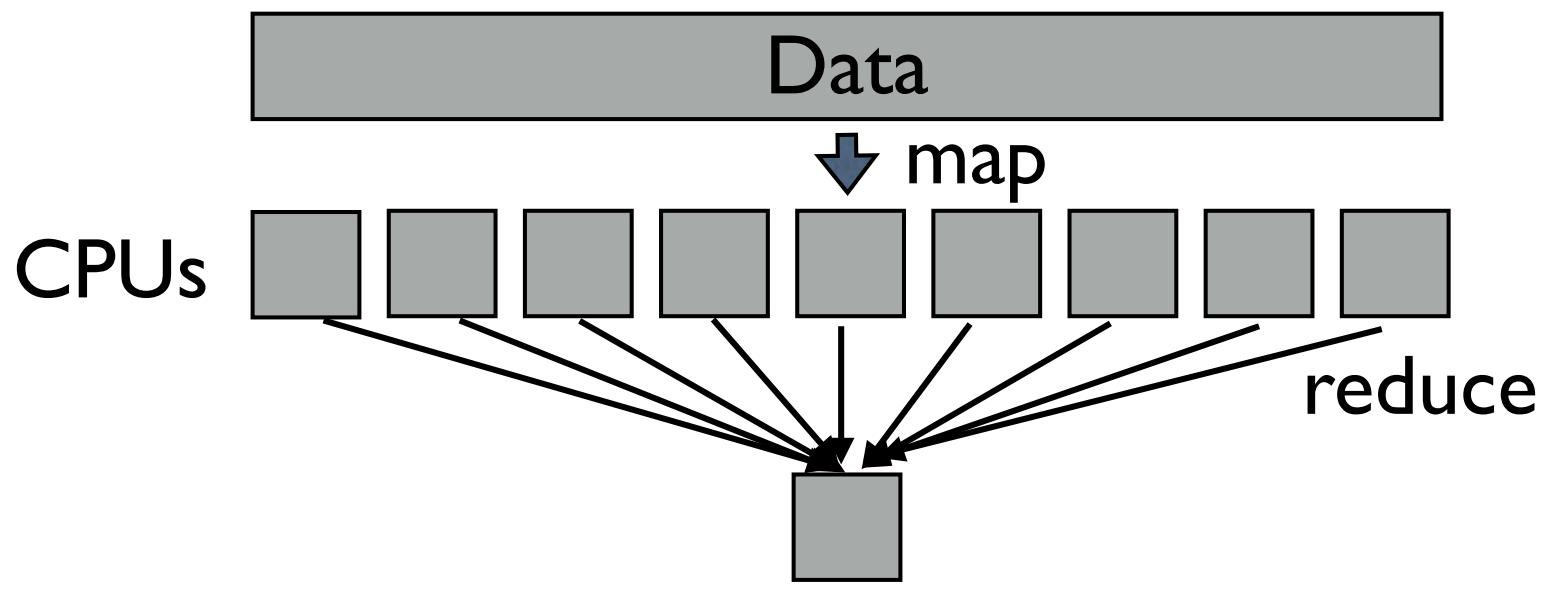
\includegraphics[keepaspectratio]{images/cf6a0668dad2e3e9b5e00aa7a863fdc92f57305800bacec5cfd6b47e5c1f6738.jpg}}

• Functions are the basic building blocks

\bookmarksetup{startatroot}

\chapter{Exercise 5.3}\label{exercise-5.3}

Time : 10 Minutes

\bookmarksetup{startatroot}

\chapter{Returning Functions}\label{returning-functions}

Consider the following function

\begin{Shaded}
\begin{Highlighting}[]
\KeywordTok{def}\NormalTok{ add(x, y):}
    \KeywordTok{def}\NormalTok{ do\_add():}
        \BuiltInTok{print}\NormalTok{(}\SpecialStringTok{f\textquotesingle{} }\SpecialCharTok{\{}\NormalTok{x}\SpecialCharTok{\}}\SpecialStringTok{ + }\SpecialCharTok{\{}\NormalTok{y}\SpecialCharTok{\}}\SpecialStringTok{ {-}\textgreater{} }\SpecialCharTok{\{}\NormalTok{x}\OperatorTok{+}\NormalTok{y}\SpecialCharTok{\}}\SpecialStringTok{\textquotesingle{}}\NormalTok{)}
    \ControlFlowTok{return}\NormalTok{ do\_add }
\end{Highlighting}
\end{Shaded}

• A function that returns another function?

\begin{Shaded}
\begin{Highlighting}[]
\NormalTok{\textgreater{}\textgreater{}\textgreater{} a = add(3,4)  }
\NormalTok{\textgreater{}\textgreater{}\textgreater{} a  }
\NormalTok{\textless{}function do\_add at 0x6a670\textgreater{}  }
\NormalTok{\textgreater{}\textgreater{}\textgreater{} a()  }
\NormalTok{3 + 4 {-}\textgreater{} 7  }
\NormalTok{\textgreater{}\textgreater{}\textgreater{} }
\end{Highlighting}
\end{Shaded}

• Notice that it works, but ponder it\ldots{}

\bookmarksetup{startatroot}

\chapter{Nested Scopes}\label{nested-scopes}

Observe how the inner function refers to variables defined by the outer
function

\begin{Shaded}
\begin{Highlighting}[]
\KeywordTok{def}\NormalTok{ add(x, y):}
    \KeywordTok{def}\NormalTok{ do\_add():}
        \BuiltInTok{print}\NormalTok{(}\SpecialStringTok{f\textquotesingle{} }\SpecialCharTok{\{}\NormalTok{x}\SpecialCharTok{\}}\SpecialStringTok{ + }\SpecialCharTok{\{}\NormalTok{y}\SpecialCharTok{\}}\SpecialStringTok{ {-}\textgreater{} }\SpecialCharTok{\{}\NormalTok{x}\OperatorTok{+}\NormalTok{y}\SpecialCharTok{\}}\SpecialStringTok{\textquotesingle{}}\NormalTok{)}
    \ControlFlowTok{return}\NormalTok{ do\_add }
\end{Highlighting}
\end{Shaded}

Further observe that those variables are somehow kept alive after add()
has finished

\begin{Shaded}
\begin{Highlighting}[]
\NormalTok{\textgreater{}\textgreater{}\textgreater{} a = add(3,4)  }
\NormalTok{\textgreater{}\textgreater{}\textgreater{} a  }
\NormalTok{\textless{}function do\_add at 0x6a670\textgreater{}  }
\NormalTok{\textgreater{}\textgreater{}\textgreater{} a()  }
\NormalTok{3 + 4 {-}\textgreater{} 7  }
\NormalTok{Where are the x,y values coming from? }
\end{Highlighting}
\end{Shaded}

\bookmarksetup{startatroot}

\chapter{Closures}\label{closures}

If an inner function is returned as a result, the inner function is
known as a ``closure''

\begin{Shaded}
\begin{Highlighting}[]
\KeywordTok{def}\NormalTok{ add(x, y):}
    \KeywordTok{def}\NormalTok{ do\_add():}
        \BuiltInTok{print}\NormalTok{(}\SpecialStringTok{f\textquotesingle{} }\SpecialCharTok{\{}\NormalTok{x}\SpecialCharTok{\}}\SpecialStringTok{ + }\SpecialCharTok{\{}\NormalTok{y}\SpecialCharTok{\}}\SpecialStringTok{ {-}\textgreater{} }\SpecialCharTok{\{}\NormalTok{x}\OperatorTok{+}\NormalTok{y}\SpecialCharTok{\}}\SpecialStringTok{\textquotesingle{}}\NormalTok{) }
\end{Highlighting}
\end{Shaded}

Essential feature : A ``closure'' retains the values of all variables
needed for the function to run properly later on

\bookmarksetup{startatroot}

\chapter{Closures}\label{closures-1}

• To make it work, references to the outer variables (bound variables)
get carried along with the function

\begin{Shaded}
\begin{Highlighting}[]
\KeywordTok{def}\NormalTok{ add(x, y):}
    \KeywordTok{def}\NormalTok{ do\_add():}
        \BuiltInTok{print}\NormalTok{(}\SpecialStringTok{f\textquotesingle{} }\SpecialCharTok{\{}\NormalTok{x}\SpecialCharTok{\}}\SpecialStringTok{ + }\SpecialCharTok{\{}\NormalTok{y}\SpecialCharTok{\}}\SpecialStringTok{ {-}\textgreater{} }\SpecialCharTok{\{}\NormalTok{x}\OperatorTok{+}\NormalTok{y}\SpecialCharTok{\}}\SpecialStringTok{\textquotesingle{}}\NormalTok{)}
    \ControlFlowTok{return}\NormalTok{ do\_add}
\OperatorTok{\textgreater{}\textgreater{}\textgreater{}}\NormalTok{ a }\OperatorTok{=}\NormalTok{ add(}\DecValTok{3}\NormalTok{, }\DecValTok{4}\NormalTok{)}
\OperatorTok{\textgreater{}\textgreater{}\textgreater{}}\NormalTok{ a.\_closure\_}
\NormalTok{(}\OperatorTok{\textless{}}\NormalTok{cell at }\BaseNTok{0x54f30}\NormalTok{: }\BuiltInTok{int} \BuiltInTok{object}\NormalTok{ at }\BaseNTok{0x54fe0}\OperatorTok{\textgreater{}}\NormalTok{, }\OperatorTok{\textless{}}\NormalTok{cell at }\BaseNTok{0x54fd0}\NormalTok{: }\BuiltInTok{int} \BuiltInTok{object}\NormalTok{ at }\BaseNTok{0x54f60}\OperatorTok{\textgreater{}}\NormalTok{) }\OperatorTok{\textgreater{}\textgreater{}\textgreater{}}\NormalTok{ a.\_closure\_[}\DecValTok{0}\NormalTok{].cell相关内容}
\OperatorTok{\textgreater{}\textgreater{}\textgreater{}}\NormalTok{ a.\_closure\_[}\DecValTok{1}\NormalTok{].cell相关内容 }
\end{Highlighting}
\end{Shaded}

\bookmarksetup{startatroot}

\chapter{Closures}\label{closures-2}

\bookmarksetup{startatroot}

\chapter{Closures only capture used
variables}\label{closures-only-capture-used-variables}

\begin{Shaded}
\begin{Highlighting}[]
\KeywordTok{def}\NormalTok{ add(x, y):}
\NormalTok{    result }\OperatorTok{=}\NormalTok{ x }\OperatorTok{+}\NormalTok{ y}
    \KeywordTok{def}\NormalTok{ get\_result():}
        \ControlFlowTok{return}\NormalTok{ result}
    \ControlFlowTok{return}\NormalTok{ get\_result }
\end{Highlighting}
\end{Shaded}

\begin{Shaded}
\begin{Highlighting}[]
\NormalTok{\textgreater{}\textgreater{}\textgreater{} a = add(3, 4)  }
\NormalTok{\textgreater{}\textgreater{}\textgreater{} a.\_closure\_  }
\NormalTok{(\textless{}cell at 0x10bb52708: int object at 0x10b5d3610\textgreater{},)  }
\NormalTok{\textgreater{}\textgreater{}\textgreater{} a.\_closure\_[0].cell相关内容  }
\NormalTok{7  }
\NormalTok{\textgreater{}\textgreater{}\textgreater{} }
\end{Highlighting}
\end{Shaded}

\bookmarksetup{startatroot}

\chapter{Carefully observe: x and y are not included (not needed in the
function
body)}\label{carefully-observe-x-and-y-are-not-included-not-needed-in-the-function-body}

\bookmarksetup{startatroot}

\chapter{Closures and Mutability}\label{closures-and-mutability}

• Closure variables are mutable (nonlocal decl)

\begin{Shaded}
\begin{Highlighting}[]
\KeywordTok{def}\NormalTok{ counter(n):}
    \KeywordTok{def}\NormalTok{ incr():}
        \KeywordTok{nonlocal}\NormalTok{ n}
\NormalTok{        n }\OperatorTok{+=} \DecValTok{1}
        \ControlFlowTok{return}\NormalTok{ n}
    \ControlFlowTok{return}\NormalTok{ incr }
\end{Highlighting}
\end{Shaded}

\begin{Shaded}
\begin{Highlighting}[]
\NormalTok{\textgreater{}\textgreater{}\textgreater{} c = counter(10)  }
\NormalTok{\textgreater{}\textgreater{}\textgreater{} c()  }
\NormalTok{11  }
\NormalTok{\textgreater{}\textgreater{}\textgreater{} c()  }
\NormalTok{12  }
\NormalTok{\textgreater{}\textgreater{}\textgreater{} }
\end{Highlighting}
\end{Shaded}

Can be used to hold mutable internal state, much like an object or class

\bookmarksetup{startatroot}

\chapter{Using Closures}\label{using-closures}

• Closures are an essential feature of Python\\
Common applications:

• Alternate evaluation (e.g., ``delayed evaluation)\\
Callback functions\\
Code creation (''macros'')

\bookmarksetup{startatroot}

\chapter{Exercise 5.4}\label{exercise-5.4}

Time : 10 Minutes

\bookmarksetup{startatroot}

\chapter{Function Error Checking}\label{function-error-checking}

• As you know, exceptions indicate errors raise RuntimeError(``You're
dead'')\\
Exceptions can be caught

\begin{Shaded}
\begin{Highlighting}[]
\ControlFlowTok{try}\OperatorTok{:}\NormalTok{ statements except RuntimeError }\ImportTok{as}\NormalTok{ e}\OperatorTok{:}\NormalTok{ \# Handle the runtime error }
\end{Highlighting}
\end{Shaded}

The mechanics of exception handling is usually straightforward, but
proper usage is often a lot trickier than it looks

\bookmarksetup{startatroot}

\chapter{What Exceptions to Handle?}\label{what-exceptions-to-handle}

Functions should only handle exceptions where recovery is possible (and
makes sense):

\begin{Shaded}
\begin{Highlighting}[]
\KeywordTok{def}\NormalTok{ read\_csv(filename):}
\NormalTok{    f }\OperatorTok{=} \BuiltInTok{open}\NormalTok{(filename)}
    \ControlFlowTok{for}\NormalTok{ row }\KeywordTok{in}\NormalTok{ csv}\OperatorTok{{-}}\NormalTok{reader(f):}
        \ControlFlowTok{try}\NormalTok{:}
\NormalTok{            name }\OperatorTok{=}\NormalTok{ row[}\DecValTok{0}\NormalTok{]}
\NormalTok{            shares }\OperatorTok{=} \BuiltInTok{int}\NormalTok{(row[}\DecValTok{1}\NormalTok{])}
\NormalTok{            price }\OperatorTok{=} \BuiltInTok{float}\NormalTok{(row[}\DecValTok{2}\NormalTok{])}
        \ControlFlowTok{except} \PreprocessorTok{ValueError} \ImportTok{as}\NormalTok{ e:}
            \BuiltInTok{print}\NormalTok{(}\StringTok{\textquotesingle{}Bad row: \textquotesingle{}}\NormalTok{, row)}
        \ControlFlowTok{continue}
\NormalTok{    ... }
\end{Highlighting}
\end{Shaded}

• Let all other exceptions propagate--they usually indicate a more
serious problem

\bookmarksetup{startatroot}

\chapter{Example}\label{example-3}

Don't worry about things like this

\begin{Shaded}
\begin{Highlighting}[]
\NormalTok{\textgreater{}\textgreater{}\textgreater{} read\_csv(\textquotesingle{}bogus.csv\textquotesingle{})   }
\NormalTok{Traceback (most recent call last): File "\textless{}stdin\textgreater{}", line 1, in \textless{}module\textgreater{} File "reader.py", line 10, in read\_csv f = open(filename)   }
\NormalTok{FileNotFoundError: [Errno 2] No such file or directory: \textquotesingle{}bogus.csv\textquotesingle{}   }
\NormalTok{\textgreater{}\textgreater{}\textgreater{} }
\end{Highlighting}
\end{Shaded}

There is no sensible recovery. The failure is someone else's problem.

\bookmarksetup{startatroot}

\chapter{Catching All Errors}\label{catching-all-errors}

Never catch all exceptions unless you report/ record the actual
exception that occurred

\begin{Shaded}
\begin{Highlighting}[]
\ControlFlowTok{try}\NormalTok{: }\CommentTok{\# Some complicated operation except Exception as e: print("Sorry, it didn\textquotesingle{}t work.") print("Reason:", e) }
\end{Highlighting}
\end{Shaded}

Not reporting actual exception information is the fastest way to create
undebuggable code

\bookmarksetup{startatroot}

\chapter{Ignoring Errors}\label{ignoring-errors}

\bookmarksetup{startatroot}

\chapter{No! No! No!}\label{no-no-no}

try: \# Some complicated operation except Exception: pass

\bookmarksetup{startatroot}

\chapter{Argh!!!! Boom!}\label{argh-boom}

try: \# Some complicated operation • except Exception: \# !! TODO pass

\bookmarksetup{startatroot}

\chapter{Catastrophic failures are often a result of exception handling
gone terribly
wrong.}\label{catastrophic-failures-are-often-a-result-of-exception-handling-gone-terribly-wrong.}

\pandocbounded{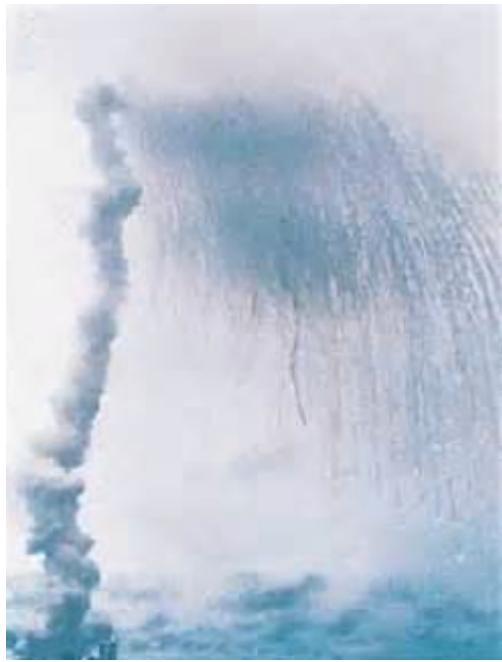
\includegraphics[keepaspectratio]{images/00e44ed599ecac58a7bc499129a3fbd34ea7a9f759f58d9a5b76ef1a3621e6d8.jpg}}\\
Ariane 5

\bookmarksetup{startatroot}

\chapter{Reraising Exceptions}\label{reraising-exceptions}

\bookmarksetup{startatroot}

\chapter{Log/re-raise}\label{logre-raise}

\begin{Shaded}
\begin{Highlighting}[]
\ControlFlowTok{try}\NormalTok{: }\CommentTok{\# Some complicated operation except Exception as e: print("Sorry, it didn\textquotesingle{}t work.") print("Reason:", e) raise }
\end{Highlighting}
\end{Shaded}

Useful if you want to do something with the exception, but allow it to
propagate

\bookmarksetup{startatroot}

\chapter{Wrapped Exceptions}\label{wrapped-exceptions}

• Wrapping an exception in another exception

try:

except Exception as e:

raise TaskError(`It failed') from e

Unwrapping it later

try:

except TaskError as e: print(``It didn't seem to work.'')
print(``Reason:'', e.\_\_cause\_\_)

Forms an exception chain

\bookmarksetup{startatroot}

\chapter{Managing Resources}\label{managing-resources}

• Take care to manage system resources correctly

\begin{Shaded}
\begin{Highlighting}[]
\KeywordTok{def}\NormalTok{ read\_data(filename):}
\NormalTok{    f }\OperatorTok{=} \BuiltInTok{open}\NormalTok{(filename)}
    \ControlFlowTok{try}\NormalTok{:}
\NormalTok{        ... do whatever ...}
    \ControlFlowTok{finally}\NormalTok{:}
\NormalTok{        f.close() }
\end{Highlighting}
\end{Shaded}

• A more modern version (context manager)

\begin{Shaded}
\begin{Highlighting}[]
\KeywordTok{def}\NormalTok{ read\_data(filename):}
\NormalTok{    f }\OperatorTok{=} \BuiltInTok{open}\NormalTok{(filename)}
    \ControlFlowTok{with}\NormalTok{ f:}
\NormalTok{        ... do whatever ... }
\end{Highlighting}
\end{Shaded}

Failure to do this might cause leaky file descriptors, deadlock, or
other problems

\bookmarksetup{startatroot}

\chapter{What Exceptions to Raise?}\label{what-exceptions-to-raise}

• Applications should have their own exceptions

class ApplicationError(Exception): pass

class SomeOtherError(ApplicationError): pass

Issue: How do you distinguish between programming mistakes and
exceptions that you meant to raise?\\
Reserve Python's built-in exceptions for programming mistakes. Catch,
don't raise.

\bookmarksetup{startatroot}

\chapter{Return Codes}\label{return-codes}

Don't use return codes (usually)

\begin{Shaded}
\begin{Highlighting}[]
\KeywordTok{def}\NormalTok{ read\_data(filename):}
    \CommentTok{\# Some complicated thing}
\NormalTok{    ...}
    \ControlFlowTok{if}\NormalTok{ error:}
        \ControlFlowTok{return} \OperatorTok{{-}}\DecValTok{1}  \CommentTok{\# Oops}
    \ControlFlowTok{else}\NormalTok{:}
        \ControlFlowTok{return}\NormalTok{ result }
\end{Highlighting}
\end{Shaded}

Return codes are not the ``standard'' way of signaling errors in
Python\\
Callers will often forget and program will crash for a different reason
later.

\bookmarksetup{startatroot}

\chapter{Logging}\label{logging}

• Use logging for recording diagnostics

\begin{Shaded}
\begin{Highlighting}[]
\ImportTok{import}\NormalTok{ logging  }
\NormalTok{log }\OperatorTok{=}\NormalTok{ logging.getLogger(\_name\_\_) }
\end{Highlighting}
\end{Shaded}

\begin{Shaded}
\begin{Highlighting}[]
\KeywordTok{def}\NormalTok{ read\_data(filename):}
\NormalTok{    ...}
    \ControlFlowTok{try}\NormalTok{:}
\NormalTok{        name }\OperatorTok{=}\NormalTok{ row[}\DecValTok{0}\NormalTok{]}
\NormalTok{        shares }\OperatorTok{=} \BuiltInTok{int}\NormalTok{(row[}\DecValTok{1}\NormalTok{])}
\NormalTok{        price }\OperatorTok{=} \BuiltInTok{float}\NormalTok{(row[}\DecValTok{2}\NormalTok{])}
    \ControlFlowTok{except} \PreprocessorTok{ValueError} \ImportTok{as}\NormalTok{ e:}
\NormalTok{        log.warn(}\StringTok{"Bad row: }\SpecialCharTok{\%s}\StringTok{"}\NormalTok{, row)}
\NormalTok{        log.debug(}\StringTok{"Reason: }\SpecialCharTok{\%s}\StringTok{"}\NormalTok{, e) }
\end{Highlighting}
\end{Shaded}

• Usually a better option than print() functions

\bookmarksetup{startatroot}

\chapter{Exercise 5.5}\label{exercise-5.5}

Time : 15 Minutes

\bookmarksetup{startatroot}

\chapter{Testing Rocks, Debugging
Sucks}\label{testing-rocks-debugging-sucks}

• What else is there to say?\\
Dynamic nature of Python makes testing critically important to most
applications\\
• There is no compiler to find your bugs\\
Only way to find bugs is to run the code and make sure you exercise all
of its features

\bookmarksetup{startatroot}

\chapter{Example Code}\label{example-code}

• Suppose you have this function

simple.py\\
def add(x,y): Addx and y. return \(\mathbf{x} + \mathbf{y}\)
\textgreater\textgreater\textgreater add(2,2)\\
4\\
\textgreater\textgreater\textgreater add(`hello',`world') `helloworld'\\
\textgreater\textgreater\textgreater{}

Let's test it

\bookmarksetup{startatroot}

\chapter{Assertions/Contracts}\label{assertionscontracts}

\bookmarksetup{startatroot}

\chapter{• Assertions are runtime
checks}\label{assertions-are-runtime-checks}

\begin{Shaded}
\begin{Highlighting}[]
\KeywordTok{def}\NormalTok{ add(x, y):}
\NormalTok{    ...}
\NormalTok{    Adds x }\KeywordTok{and}\NormalTok{ y}
\NormalTok{    ...}
    \ControlFlowTok{assert} \BuiltInTok{isinstance}\NormalTok{(x, }\BuiltInTok{int}\NormalTok{)}
    \ControlFlowTok{assert} \BuiltInTok{isinstance}\NormalTok{(y, }\BuiltInTok{int}\NormalTok{)}
    \ControlFlowTok{return}\NormalTok{ x }\OperatorTok{+}\NormalTok{ y }
\end{Highlighting}
\end{Shaded}

\bookmarksetup{startatroot}

\chapter{Function will fail on bad
input}\label{function-will-fail-on-bad-input}

\begin{Shaded}
\begin{Highlighting}[]
\NormalTok{\textgreater{}\textgreater{}\textgreater{} add(2, 3)  }
\NormalTok{5  }
\NormalTok{\textgreater{}\textgreater{}\textgreater{} add(\textquotesingle{}2\textquotesingle{}, \textquotesingle{}3\textquotesingle{})  }
\NormalTok{Traceback (most recent call last):  }
\NormalTok{...  }
\NormalTok{AssertionError  }
\NormalTok{\textgreater{}\textgreater{}\textgreater{} }
\end{Highlighting}
\end{Shaded}

\bookmarksetup{startatroot}

\chapter{Assertions/Contracts}\label{assertionscontracts-1}

• Assertions are not meant to check user inputs\\
Should validate program invariants (internal conditions that must always
hold true)\\
Failure indicates a programming error and assign blame (e.g., to the
caller)\\
Can be disabled (python -O)

bash \% python3 -O prog.py

\bookmarksetup{startatroot}

\chapter{unittest Module}\label{unittest-module}

Built-in module used for testing\\
• Used by the standard library\\
Commonly used in other applications\\
Will briefly illustrate

\bookmarksetup{startatroot}

\chapter{Using unittest}\label{using-unittest}

• First, you create a separate file

\begin{Shaded}
\begin{Highlighting}[]
\CommentTok{\# testsimple.py}
\ImportTok{import}\NormalTok{ simple}
\ImportTok{import}\NormalTok{ unittest }
\end{Highlighting}
\end{Shaded}

• Then you define testing classes

\begin{Shaded}
\begin{Highlighting}[]
\NormalTok{class TestAdd(unittest.TestCase): }
\end{Highlighting}
\end{Shaded}

• They must inherit from unittest.TestCase

\bookmarksetup{startatroot}

\chapter{Using unittest}\label{using-unittest-1}

\bookmarksetup{startatroot}

\chapter{Define testing methods}\label{define-testing-methods}

class TestAdd(unittest.TestCase): def test.simple(self): \#Test with
simple integer arguments r \(=\) simple.add(2,2) self.assertEqual(r,5)

\begin{Shaded}
\begin{Highlighting}[]
\KeywordTok{def}\NormalTok{ test\_str(}\VariableTok{self}\NormalTok{):}
    \CommentTok{\# Test with strings}
\NormalTok{    r }\OperatorTok{=}\NormalTok{ simple.add(}\StringTok{\textquotesingle{}hello\textquotesingle{}}\NormalTok{, }\StringTok{\textquotesingle{}world\textquotesingle{}}\NormalTok{)}
    \VariableTok{self}\NormalTok{.assertEqual(r, }\StringTok{\textquotesingle{}helloworld\textquotesingle{}}\NormalTok{) }
\end{Highlighting}
\end{Shaded}

• Each method must start with ``test\ldots{}''

\bookmarksetup{startatroot}

\chapter{Using unittest}\label{using-unittest-2}

\bookmarksetup{startatroot}

\chapter{Each test uses special
assertions}\label{each-test-uses-special-assertions}

\bookmarksetup{startatroot}

\chapter{Assert that expr is True
self.assertTrue(expr)}\label{assert-that-expr-is-true-self.asserttrueexpr}

\bookmarksetup{startatroot}

\chapter{Assert that x == y
self.assertEqual(x,y)}\label{assert-that-x-y-self.assertequalxy}

\bookmarksetup{startatroot}

\chapter{Assert that x is near y
self.assertAlmostEqual(x,y,places)}\label{assert-that-x-is-near-y-self.assertalmostequalxyplaces}

\bookmarksetup{startatroot}

\chapter{Assert that an exception is raised with
self.assertRaises(SomeError): statement1 statement2
..}\label{assert-that-an-exception-is-raised-with-self.assertraisessomeerror-statement1-statement2-..}

\bookmarksetup{startatroot}

\chapter{There are others}\label{there-are-others}

\bookmarksetup{startatroot}

\chapter{Running unittests}\label{running-unittests}

• To run tests, add the following code

\bookmarksetup{startatroot}

\chapter{testsimple.py}\label{testsimple.py}

if \_name \_main\_\_' unittest.main()

Then run Python on the test file

bash \% python3 testsimple.py F.

FAIL: test\_simple (\textbf{main}.TestAdd)

Traceback (most recent call last): File ``testsimple.py'', line 8, in
test\_simple self.assertEqual(r, 5)

AssertionError: 4 != 5

Ran 2 tests in 0.000s

FAILED (failures=1)

\bookmarksetup{startatroot}

\chapter{unittest comments}\label{unittest-comments}

Can grow to be quite complicated for large applications\\
The unittest module has a huge number of options related to test
runners, collection of results, and other aspects of testing (consult
documentation for details)\\
• Look at pytest as an alternative

\bookmarksetup{startatroot}

\chapter{Exercise 5.6}\label{exercise-5.6}

Time : 15 Minutes

\bookmarksetup{startatroot}

\chapter{Section 6}\label{section-6}

\bookmarksetup{startatroot}

\chapter{Working with Code}\label{working-with-code}

\bookmarksetup{startatroot}

\chapter{Overview}\label{overview-3}

• Advanced function usage/definition\\
Introspection\\
• Code generation (eval, exec)\\
Callables

\bookmarksetup{startatroot}

\chapter{Function Arguments}\label{function-arguments}

• Functions operate on passed arguments

def func(x,y,z): statements

arguments

There are two calling styles

a = func(1,2,3)

\bookmarksetup{startatroot}

\chapter{Positional arguments}\label{positional-arguments}

a \(=\) func(x=1,y=2,z=3)

\bookmarksetup{startatroot}

\chapter{Keyword arguments}\label{keyword-arguments-1}

• You can mix the two styles

\[
a = \operatorname {f u n c} (1, z = 3, y = 2)
\]

Positional args always go first. Each argument gets one and only one
value

\bookmarksetup{startatroot}

\chapter{Variable Arguments}\label{variable-arguments}

• Function that accepts any number of args

def func(x, *args):

• Here, the arguments get passed as a tuple

\pandocbounded{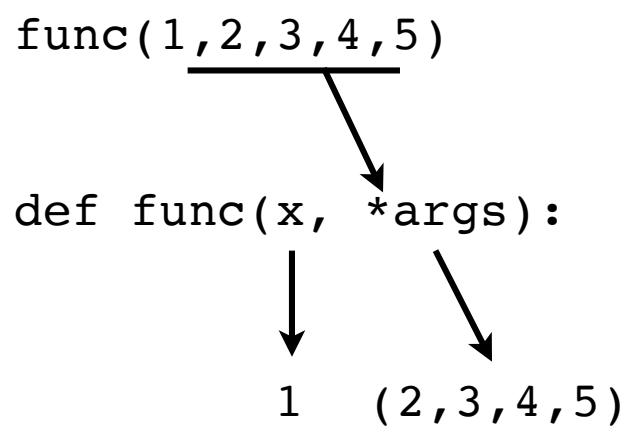
\includegraphics[keepaspectratio]{images/c88959b68a7d679dbc1fbbd3fe72781f70bbb228e0032b44c77905d0e25bcca9.jpg}}

\bookmarksetup{startatroot}

\chapter{Variable Arguments}\label{variable-arguments-1}

Function that accepts any keyword args

def func(x, y, **kwargs):

Extra keywords get passed in a dict

\begin{Shaded}
\begin{Highlighting}[]
\NormalTok{func(}\DecValTok{2}\NormalTok{, }\DecValTok{3}\NormalTok{, flag}\OperatorTok{=}\VariableTok{True}\NormalTok{, mode}\OperatorTok{=}\StringTok{"fast"}\NormalTok{, header}\OperatorTok{=}\StringTok{"debug"}\NormalTok{)}
\KeywordTok{def}\NormalTok{ func(x, y, }\OperatorTok{**}\NormalTok{kwargs):}
\NormalTok{    \{}
        \StringTok{\textquotesingle{}flag\textquotesingle{}}\NormalTok{: }\VariableTok{True}\NormalTok{,}
        \StringTok{\textquotesingle{}mode\textquotesingle{}}\NormalTok{: }\StringTok{\textquotesingle{}fast\textquotesingle{}}\NormalTok{,}
        \StringTok{\textquotesingle{}header\textquotesingle{}}\NormalTok{: }\StringTok{\textquotesingle{}debug\textquotesingle{}} 
\end{Highlighting}
\end{Shaded}

\bookmarksetup{startatroot}

\chapter{Variable Arguments}\label{variable-arguments-2}

• A function that takes any arguments

def func(*args, **kwargs): statements

• This will accept any combination of positional or keyword arguments\\
Sometimes used when writing wrappers or when you want to pass arguments
through to another function

\bookmarksetup{startatroot}

\chapter{Passing Tuples and Dicts}\label{passing-tuples-and-dicts}

• Tuples can expand into function args

\[
\begin{array}{l} \text {a r g s} = (2, 3, 4) \\ \operatorname {f u n c} (1, * \text {a r g s}) \quad \# \text {S a m e a s f u n c} (1, 2, 3, 4) \\ \end{array}
\]

• Dictionaries can expand to keyword args

kwargs \(=\) \{ color': `red', delimiters': `,', width'：400\}

\begin{Shaded}
\begin{Highlighting}[]
\NormalTok{func(data, **kwargs) }
\end{Highlighting}
\end{Shaded}

\begin{Shaded}
\begin{Highlighting}[]
\NormalTok{Same as func(data,color=\textquotesingle{}red\textquotesingle{}, delimiter=\textquotesingle{},\textquotesingle{}width=400) }
\end{Highlighting}
\end{Shaded}

\bookmarksetup{startatroot}

\chapter{Exercise 6.1}\label{exercise-6.1}

Time : 20 minutes

\bookmarksetup{startatroot}

\chapter{Scoping Rules}\label{scoping-rules}

• Programs assign values to variables

x = value \# Global variable

def func():

y = value \# Local variable

• Python manages variables in two scopes

Globals (assigned outside functions)\\
• Locals (assignments inside functions)

\bookmarksetup{startatroot}

\chapter{Statement Execution}\label{statement-execution}

• All statements execute within two scopes (even statements not part of
a function)\\
Global scope is always the module in which a function is defined\\
• Local scope is either private to a function or the same as the global
scope (for statements executed at module level)

\bookmarksetup{startatroot}

\chapter{Modifying Globals}\label{modifying-globals}

• If you want to modify a global variable you must declare it as such in
the function

\[
\textbf {x} = 4 2
\]

def func(): global x x = 37

global declaration must appear before use\\
• Only necessary for globals that will be modified (globals are already
readable)

\bookmarksetup{startatroot}

\chapter{globals() and locals()}\label{globals-and-locals}

globals() - Give you a dictionary representing the contents of global
scope\\
locals() - Gives you a dictionary representing the contents of local
scope\\
Can use these to inspect the environment in which a statement will
execute

\bookmarksetup{startatroot}

\chapter{builtins module}\label{builtins-module}

Built-in functions are in a special module\\
Consulted last when looking up names

\begin{quote}
\begin{quote}
\begin{quote}
abs(-45)\\
45\\
import builtins\\
builtins.abs(-45)\\
45
\end{quote}
\end{quote}
\end{quote}

• You can modify it (but probably not advised)

\begin{quote}
\begin{quote}
\begin{quote}
builtins.pi \(=\) 3.1415926\\
pi\\
3.1415926
\end{quote}
\end{quote}
\end{quote}

\bookmarksetup{startatroot}

\chapter{Exercise 6.2}\label{exercise-6.2}

Time : 15 minutes

\bookmarksetup{startatroot}

\chapter{Function Objects}\label{function-objects}

When you define a function, the function itself becomes a kind of object
that you can manipulate\\
Can assign to variables, place in containers, pass around as data,
etc.\\
Functions can also be inspected

\bookmarksetup{startatroot}

\chapter{Documentation Strings}\label{documentation-strings}

First line of function may be string

def func(a, b): `This function does something.'

• The doc string is stored in \textbf{doc}
\textgreater\textgreater\textgreater{} func.\_\emph{doc} `This function
does something.' \textgreater\textgreater\textgreater{}\\
Help tools look at \textbf{doc}, but other programs might examine it for
various purposes (testing, etc.)

\bookmarksetup{startatroot}

\chapter{Annotations/Type Hints}\label{annotationstype-hints}

• Arguments and return might be annotated

def func(a:int, b:int) -\textgreater{} int:

Stored in \_annotations

\begin{quote}
\begin{quote}
\begin{quote}
func.\_\_annotations \{`a': \textless class `int'\textgreater, `b':
\textless class `int'\textgreater, `return': \textless class
`int'\textgreater\} \textgreater\textgreater\textgreater{}
\end{quote}
\end{quote}
\end{quote}

Annotations do nothing--purely informational for other code that might
want to look at them.

\bookmarksetup{startatroot}

\chapter{Function Attributes}\label{function-attributes}

Little known fact : You can attach arbitrary attributes to a function

def func(a, b): `This function does something.'

func.threadsafe \(=\) False func.blah = 42

Under the hood, each function has a dictionary (\textbf{dict}) that
holds these values\\
• Useful for code that manipulates functions

\bookmarksetup{startatroot}

\chapter{Function Inspection}\label{function-inspection}

Almost every aspect of a function can be inspected if you know where to
look

\begin{Shaded}
\begin{Highlighting}[]
\KeywordTok{def}\NormalTok{ func(a, b, c}\OperatorTok{=}\DecValTok{42}\NormalTok{):}
    \CommentTok{\textquotesingle{}This function does something.\textquotesingle{}} 
\end{Highlighting}
\end{Shaded}

• Use the dir() function to see more

\bookmarksetup{startatroot}

\chapter{inspect Module}\label{inspect-module}

• Use the inspect module to get details about functions in a more useful
form

def func(a, b, \(\mathtt { C } = 4 2\) ):

\begin{quote}
\begin{quote}
\begin{quote}
import inspect
\end{quote}
\end{quote}
\end{quote}

\begin{quote}
\begin{quote}
\begin{quote}
sig \(=\) inspect.signature(func)
\end{quote}
\end{quote}
\end{quote}

\begin{quote}
\begin{quote}
\begin{quote}
print(sig)
\end{quote}
\end{quote}
\end{quote}

(a, b, \(\mathtt { C } = 4 2\) )

\begin{quote}
\begin{quote}
\begin{quote}
list(sig.parameters)
\end{quote}
\end{quote}
\end{quote}

{[}`a', `b', `c'{]}

\begin{quote}
\begin{quote}
\begin{quote}
sig.parameters{[}`c'{]}.default
\end{quote}
\end{quote}
\end{quote}

42

\begin{quote}
\begin{quote}
\begin{quote}
\end{quote}
\end{quote}
\end{quote}

• Many more module features (not shown)

\bookmarksetup{startatroot}

\chapter{Signature Binding}\label{signature-binding}

Signatures can be bound to *args, **kwargs

sig \(=\) inspect.signature(some\_func)

args = (1, 2)

kwargs = \{`c': 10\}

bound \(=\) sig.bind(*args, **kwargs)

for name, val in bound.arguments.items():

print(name, `=', val)

Performs all error checking\\
• Might simplify code using *args, **kwargs

\bookmarksetup{startatroot}

\chapter{Exercise 6.3}\label{exercise-6.3}

Time : 15 minutes

\bookmarksetup{startatroot}

\chapter{eval() and exec()}\label{eval-and-exec}

eval(code) - Evaluates an expression

\begin{Shaded}
\begin{Highlighting}[]
\NormalTok{\textgreater{}\textgreater{}\textgreater{} x = 10 }
\end{Highlighting}
\end{Shaded}

\begin{Shaded}
\begin{Highlighting}[]
\NormalTok{\textgreater{}\textgreater{}\textgreater{}eval(\textquotesingle{}3\textbackslash{}*x{-}2\textquotesingle{}) }
\end{Highlighting}
\end{Shaded}

\begin{Shaded}
\begin{Highlighting}[]
\NormalTok{28 }
\end{Highlighting}
\end{Shaded}

\begin{Shaded}
\begin{Highlighting}[]
\NormalTok{\textgreater{}\textgreater{}\textgreater{} }
\end{Highlighting}
\end{Shaded}

exec(code) - Executes arbitrary statements

\begin{Shaded}
\begin{Highlighting}[]
\NormalTok{\textgreater{}\textgreater{}\textgreater{} exec(\textquotesingle{}for i in range(5): print(i)\textquotesingle{}) }
\end{Highlighting}
\end{Shaded}

\begin{Shaded}
\begin{Highlighting}[]
\NormalTok{0 }
\end{Highlighting}
\end{Shaded}

\begin{Shaded}
\begin{Highlighting}[]
\NormalTok{1 }
\end{Highlighting}
\end{Shaded}

\begin{Shaded}
\begin{Highlighting}[]
\NormalTok{2 }
\end{Highlighting}
\end{Shaded}

\begin{Shaded}
\begin{Highlighting}[]
\NormalTok{3 }
\end{Highlighting}
\end{Shaded}

\begin{Shaded}
\begin{Highlighting}[]
\NormalTok{4 }
\end{Highlighting}
\end{Shaded}

\begin{Shaded}
\begin{Highlighting}[]
\NormalTok{\textgreater{}\textgreater{}\textgreater{} }
\end{Highlighting}
\end{Shaded}

• Code executes in current globals()/locals()

\bookmarksetup{startatroot}

\chapter{eval() and exec()}\label{eval-and-exec-1}

Caution: Modifications to local scope are lost

\begin{Shaded}
\begin{Highlighting}[]
\NormalTok{def func():}
\NormalTok{    x = 10}
\NormalTok{    exec(\textquotesingle{}x = 15; print(x)\textquotesingle{})  \# {-}{-}{-}\textgreater{} 15}
\NormalTok{    print(x)  \# {-}{-}{-}\textgreater{} 10  ???? }
\end{Highlighting}
\end{Shaded}

eval(expr {[}, globals {[}, locals{]})\\
exec(code {[}, globals {[}, locals{]})

\begin{Shaded}
\begin{Highlighting}[]
\KeywordTok{def}\NormalTok{ func():}
\NormalTok{    x }\OperatorTok{=} \DecValTok{10}
\NormalTok{    loc }\OperatorTok{=} \BuiltInTok{locals}\NormalTok{()}
    \BuiltInTok{exec}\NormalTok{(}\StringTok{\textquotesingle{}x = 15; print(x)\textquotesingle{}}\NormalTok{, }\BuiltInTok{globals}\NormalTok{(), loc) }\CommentTok{\# {-}{-}{-}\textgreater{} 15}
\NormalTok{    x }\OperatorTok{=}\NormalTok{ loc[}\StringTok{\textquotesingle{}x\textquotesingle{}}\NormalTok{]}
    \BuiltInTok{print}\NormalTok{(x) }\CommentTok{\# {-}{-}{-}\textgreater{} 15 }
\end{Highlighting}
\end{Shaded}

\bookmarksetup{startatroot}

\chapter{eval/exec Caution}\label{evalexec-caution}

• Use these features with extreme care\\
• Overuse will likely make people hate you\\
• Tricky interaction with scoping/variables\\
• Potential security issue with untrusted inputs

\bookmarksetup{startatroot}

\chapter{Exercise 6.4}\label{exercise-6.4}

Time : 15 minutes

\bookmarksetup{startatroot}

\chapter{Callable Objects}\label{callable-objects}

You can define your own objects that emulate Python functions (e.g.,
``callables'')

\begin{Shaded}
\begin{Highlighting}[]
\KeywordTok{class}\NormalTok{ Callable: }\KeywordTok{def} \FunctionTok{\_\_call\_\_}\NormalTok{(}\VariableTok{self}\NormalTok{, }\OperatorTok{*}\NormalTok{args, }\OperatorTok{**}\NormalTok{kwargs): }\BuiltInTok{print}\NormalTok{(}\StringTok{\textquotesingle{}Calling\textquotesingle{}}\NormalTok{, args, kwargs) }
\end{Highlighting}
\end{Shaded}

• Must implement \textbf{call} special method

\begin{Shaded}
\begin{Highlighting}[]
\OperatorTok{\textgreater{}\textgreater{}\textgreater{}}\NormalTok{ c }\OperatorTok{=}\NormalTok{ Callable()}
\OperatorTok{\textgreater{}\textgreater{}\textgreater{}}\NormalTok{ c(}\DecValTok{2}\NormalTok{,}\DecValTok{3}\NormalTok{,color}\OperatorTok{=}\StringTok{\textquotesingle{}red\textquotesingle{}}\NormalTok{)}
\NormalTok{Calling (}\DecValTok{2}\NormalTok{,}\DecValTok{3}\NormalTok{) \{}\StringTok{\textquotesingle{}color\textquotesingle{}}\NormalTok{: }\StringTok{\textquotesingle{}red\textquotesingle{}}\NormalTok{\} }
\end{Highlighting}
\end{Shaded}

• Free to do anything you want in \textbf{call}

\bookmarksetup{startatroot}

\chapter{Defining Callables}\label{defining-callables}

Callable objects sometimes defined when you need to have more than just
a function (e.g., storing extra data, caching, etc.)

\begin{Shaded}
\begin{Highlighting}[]
\KeywordTok{class}\NormalTok{ Memoize: }\KeywordTok{def} \FunctionTok{\_\_init\_\_}\NormalTok{(}\VariableTok{self}\NormalTok{, func): }\VariableTok{self}\NormalTok{.\_cache }\OperatorTok{=}\NormalTok{ \{\}. }\VariableTok{self}\NormalTok{.\_func }\OperatorTok{=}\NormalTok{ func }\KeywordTok{def} \FunctionTok{\_\_call\_\_}\NormalTok{(}\VariableTok{self}\NormalTok{, }\OperatorTok{*}\NormalTok{args): }\ControlFlowTok{if}\NormalTok{ args }\KeywordTok{in} \VariableTok{self}\NormalTok{.\_cache: }\ControlFlowTok{return} \VariableTok{self}\NormalTok{.\_cache(args) r }\OperatorTok{=} \VariableTok{self}\NormalTok{.\_func(}\OperatorTok{*}\NormalTok{args) }\VariableTok{self}\NormalTok{.\_cache(args) }\OperatorTok{=}\NormalTok{ r }\ControlFlowTok{return}\NormalTok{ r }\KeywordTok{def}\NormalTok{ clear(}\VariableTok{self}\NormalTok{): }\VariableTok{self}\NormalTok{.\_cache.clear() }
\end{Highlighting}
\end{Shaded}

\bookmarksetup{startatroot}

\chapter{Exercise 6.5}\label{exercise-6.5}

Time : 15 Minutes

\bookmarksetup{startatroot}

\chapter{Section 7}\label{section-7}

\bookmarksetup{startatroot}

\chapter{Metaprogramming}\label{metaprogramming}

\bookmarksetup{startatroot}

\chapter{Introduction}\label{introduction}

• Writing programs where there is a lot of code replication is usually
problematic\\
Tedious to write\\
• Hard to maintain\\
Painful if you decide that you need to make a change (or fix a bug) in
all of that extremely repetitive code

\bookmarksetup{startatroot}

\chapter{Metaprogramming}\label{metaprogramming-1}

Metaprogramming pertains to the problem of writing code that manipulates
other code\\
Common examples:

• Macros\\
Wrappers\\
Aspects

Essentially, it's doing things to code

\bookmarksetup{startatroot}

\chapter{Python Metaprogramming}\label{python-metaprogramming}

Major features

Decorators\\
Class decorators\\
• Metaclasses

• We're going to talk about all of them\\
• They are not as difficult to grasp as you think

\bookmarksetup{startatroot}

\chapter{Decorators}\label{decorators}

• A decorator is a function that creates a wrapper around another
function\\
The wrapper is a new function that works exactly like the original
function (same arguments, same return value) except that some kind of
extra processing is carried out\\
Let's see a simple example first

\bookmarksetup{startatroot}

\chapter{Wrapper Functions}\label{wrapper-functions}

Here is a simple function:

def add(x, y): return x + y

Here is an example of a wrapper function

def logged\_add(x, y): print(`Calling add') return add(x, y)

• Example use:

\begin{quote}
\begin{quote}
\begin{quote}
add(3, 4) 7 \textgreater\textgreater\textgreater{} logged\_add(3, 4)
This extra output is created by the Calling add wrapper, but the
original function 7\textgreater\textgreater\textgreater{} is still
called to get the result
\end{quote}
\end{quote}
\end{quote}

\bookmarksetup{startatroot}

\chapter{Creating Wrappers}\label{creating-wrappers}

Insight : You can write a function that makes a wrapper around any
function

def logged(func): \#Defineawrpperfunctionaroundfunc defwrapper
\(\text{串} _ { \text{串} }\) args，**kwargs）:
print(`Calling'，func.\_name\_） return func
\(\text{串} _ { \text{串} }\) args，**kwargs) return wrapper

Usage:

\begin{Shaded}
\begin{Highlighting}[]
\NormalTok{\textgreater{}\textgreater{}\textgreater{} logged\_add = logged(add)  }
\NormalTok{\textgreater{}\textgreater{}\textgreater{} logged\_add  }
\NormalTok{\textless{}function wrapper at 0x378670\textgreater{}  }
\NormalTok{\textgreater{}\textgreater{}\textgreater{} logged\_add(3, 4)  }
\NormalTok{Calling add  }
\NormalTok{7  }
\NormalTok{\textgreater{}\textgreater{}\textgreater{} }
\end{Highlighting}
\end{Shaded}

\bookmarksetup{startatroot}

\chapter{Wrappers as Replacements}\label{wrappers-as-replacements}

• When you create a wrapper, you often want to replace the original
function with it

\begin{Shaded}
\begin{Highlighting}[]
\NormalTok{def add(x, y): return x + y }
\end{Highlighting}
\end{Shaded}

Replace add with a wrapped version add \(=\) logged(add)

• Other code continues to use the original function name, but is unaware
that a wrapper has been injected (that's the whole point)

\begin{Shaded}
\begin{Highlighting}[]
\NormalTok{\textgreater{}\textgreater{}\textgreater{} add(3, 4)  }
\NormalTok{Calling add  }
\NormalTok{7  }
\NormalTok{\textgreater{}\textgreater{}\textgreater{} }
\end{Highlighting}
\end{Shaded}

\bookmarksetup{startatroot}

\chapter{Decorator Concept}\label{decorator-concept}

• When you replace a function with a wrapper, you are usually giving the
function extra functionality\\
• This process is known as ``decoration''\\
• You are ``decorating'' a function with some extra features

\bookmarksetup{startatroot}

\chapter{Decorator Syntax}\label{decorator-syntax}

The definition of a function and wrapping almost always occur together

\begin{Shaded}
\begin{Highlighting}[]
\KeywordTok{def}\NormalTok{ add(x, y):}
    \ControlFlowTok{return}\NormalTok{ x }\OperatorTok{+}\NormalTok{ y}
\NormalTok{add }\OperatorTok{=}\NormalTok{ logged(add) }
\end{Highlighting}
\end{Shaded}

• However, it looks weird and is error prone\\
• The (\textbf{decorator?}) syntax simplifies it

\begin{Shaded}
\begin{Highlighting}[]
\NormalTok{@logged def add(x, y): return x + y }
\end{Highlighting}
\end{Shaded}

\bookmarksetup{startatroot}

\chapter{Decorator Syntax}\label{decorator-syntax-1}

• Whenever you see a decorator, a function is getting wrapped. That's
it\\
Example : In classes

\begin{Shaded}
\begin{Highlighting}[]
\KeywordTok{class}\NormalTok{ MyClass: }\KeywordTok{class}\NormalTok{ MyClass: }\OperatorTok{@}\NormalTok{staticmethod }\KeywordTok{def}\NormalTok{ bar(): }\KeywordTok{def}\NormalTok{ bar(): ... . bar }\OperatorTok{=} \BuiltInTok{staticmethod}\NormalTok{(bar) }\OperatorTok{@}\NormalTok{classmethod }\KeywordTok{def}\NormalTok{ spam(cls): }\KeywordTok{def}\NormalTok{ spam(cls): spam }\OperatorTok{=} \BuiltInTok{classmethod}\NormalTok{(spam) }\OperatorTok{@}\NormalTok{property }\KeywordTok{def}\NormalTok{ name(}\VariableTok{self}\NormalTok{): name }\OperatorTok{=} \BuiltInTok{property}\NormalTok{(name) }\KeywordTok{def}\NormalTok{ name(}\VariableTok{self}\NormalTok{): }
\end{Highlighting}
\end{Shaded}

\bookmarksetup{startatroot}

\chapter{Using Decorators}\label{using-decorators}

Use a decorator anytime you want to define a kind of ``macro'' involving
function definitions\\
• There are many possible applications

Debugging and diagnostics\\
Avoiding code replication\\
Enabling/disabling optional features

\bookmarksetup{startatroot}

\chapter{Timing Measurements}\label{timing-measurements}

\bookmarksetup{startatroot}

\chapter{• A decorator that reports execution
time}\label{a-decorator-that-reports-execution-time}

import time\\
def timethis func): def wrapper(*args, **kwargs): start \(=\)
time.time() r \(=\) func(*args, ** kwargs) end \(=\) time.time()
print(func.\_name\_,end - start) return r return wrapper

\bookmarksetup{startatroot}

\chapter{Usage:}\label{usage-1}

\begin{Shaded}
\begin{Highlighting}[]
\NormalTok{@timethis  }
\NormalTok{def bigcalculation():  }
\NormalTok{    statements  }
\NormalTok{    statements }
\end{Highlighting}
\end{Shaded}

\bookmarksetup{startatroot}

\chapter{Exercise 7.1}\label{exercise-7.1}

Time : 15 Minutes

\bookmarksetup{startatroot}

\chapter{Advanced Decorators}\label{advanced-decorators}

There are a few tricky additional details

Multiple decorators\\
Decorators and metadata\\
Decorators with arguments

\bookmarksetup{startatroot}

\chapter{Multiple Decorators}\label{multiple-decorators}

• You can apply as many decorators as you want

(\textbf{foo?})

(\textbf{bar?})

(\textbf{spam?})

def add(x, y):

return x + y

This is the same as this:

add \(=\) foo(bar(spam(add)))

To keep your sanity, it's probably not a good idea to go overboard with
it

\bookmarksetup{startatroot}

\chapter{Function Metadata}\label{function-metadata}

• When you define a function, there is some extra information stored
(name, doc strings, etc.)

\begin{Shaded}
\begin{Highlighting}[]
\KeywordTok{def}\NormalTok{ add(x, y):}
    \CommentTok{\textquotesingle{}Adds x and y\textquotesingle{}}
    \ControlFlowTok{return}\NormalTok{ x }\OperatorTok{+}\NormalTok{ y}
\OperatorTok{\textgreater{}\textgreater{}\textgreater{}}\NormalTok{ add.}\VariableTok{\_\_name\_\_}
\CommentTok{\textquotesingle{}add\textquotesingle{}}
\OperatorTok{\textgreater{}\textgreater{}\textgreater{}}\NormalTok{ add.\_\_doc\_\_}
\CommentTok{\textquotesingle{}Adds x and y\textquotesingle{}}
\OperatorTok{\textgreater{}\textgreater{}\textgreater{}} \BuiltInTok{help}\NormalTok{(add)}
\NormalTok{Help on function add }\KeywordTok{in}\NormalTok{ module \_\_main\_\_:}
\NormalTok{add(x, y)}
\NormalTok{    Adds x }\KeywordTok{and}\NormalTok{ y }
\end{Highlighting}
\end{Shaded}

\bookmarksetup{startatroot}

\chapter{The Metadata Problem}\label{the-metadata-problem}

\bookmarksetup{startatroot}

\chapter{• Decorators don't preserve
metadata}\label{decorators-dont-preserve-metadata}

(\textbf{logged?})\\
def add(x,y): `Adds x and y' return \(\mathbf{x} + \mathbf{y}\)
\textgreater\textgreater\textgreater add.\_name\_\\
`wrapper'\\
\textgreater\textgreater\textgreater add.\_doc\_\\
\textgreater\textgreater\textgreater help(add)\\
Help on function wrapper in module \_\_main\_:\\
wrapper(*args，**kwargs)\\
\textgreater\textgreater\textgreater{}

\bookmarksetup{startatroot}

\chapter{This is a problem}\label{this-is-a-problem}

\bookmarksetup{startatroot}

\chapter{Copying Metadata}\label{copying-metadata}

\bookmarksetup{startatroot}

\chapter{• Decorators should copy
metadata}\label{decorators-should-copy-metadata}

\begin{Shaded}
\begin{Highlighting}[]
\KeywordTok{def}\NormalTok{ logged(func):}
    \KeywordTok{def}\NormalTok{ wrapper(}\OperatorTok{*}\NormalTok{args, }\OperatorTok{**}\NormalTok{kwargs):}
        \BuiltInTok{print}\NormalTok{(}\StringTok{\textquotesingle{}Calling\textquotesingle{}}\NormalTok{, func.}\VariableTok{\_\_name\_\_}\NormalTok{).}
    \ControlFlowTok{return}\NormalTok{ func(}\OperatorTok{*}\NormalTok{args, }\OperatorTok{**}\NormalTok{kwargs)}
\NormalTok{manual wrapper.}\VariableTok{\_\_name\_\_} \OperatorTok{=}\NormalTok{ func.}\VariableTok{\_\_name\_\_}
\NormalTok{wrapper.\_\_doc\_\_ }\OperatorTok{=}\NormalTok{ func.\_\_doc\_\_}
\NormalTok{metadata }\ControlFlowTok{return}\NormalTok{ wrapper }
\end{Highlighting}
\end{Shaded}

\bookmarksetup{startatroot}

\chapter{\texorpdfstring{• A better solution : use
(\textbf{wraps?})}{• A better solution : use (wraps?)}}\label{a-better-solution-use-wraps}

from functools import wraps

\begin{Shaded}
\begin{Highlighting}[]
\NormalTok{Copies def logged func): metadata @wraps func) from func to def wrapper \textbackslash{}*args, \textbackslash{}*\textbackslash{}*kwargs): the wrapper print(\textquotesingle{}Calling\textquotesingle{},func.\_name\_) return func \textbackslash{}*args, \textbackslash{}*\textbackslash{}*kwargs) return wrapper }
\end{Highlighting}
\end{Shaded}

\bookmarksetup{startatroot}

\chapter{Decorators with Args}\label{decorators-with-args}

Decorators can accept arguments

\begin{Shaded}
\begin{Highlighting}[]
\NormalTok{@decorator(x, y, z) def func():}
\end{Highlighting}
\end{Shaded}

• It's mind boggling, but here's what happens def func(): \ldots{}

\begin{Shaded}
\begin{Highlighting}[]
\NormalTok{func = decorator(x, y, z) (func) }
\end{Highlighting}
\end{Shaded}

The decorator function must return a function which is called to make a
wrapper

\bookmarksetup{startatroot}

\chapter{Decorators with Args}\label{decorators-with-args-1}

Example: Logging with a custom message

\begin{Shaded}
\begin{Highlighting}[]
\KeywordTok{def}\NormalTok{ logmsg(message):}
    \KeywordTok{def}\NormalTok{ logged(func):}
        \AttributeTok{@wraps}\NormalTok{(func)}
        \KeywordTok{def}\NormalTok{ wrapper(}\OperatorTok{*}\NormalTok{args, }\OperatorTok{**}\NormalTok{kwargs):}
            \BuiltInTok{print}\NormalTok{(message.}\BuiltInTok{format}\NormalTok{(name}\OperatorTok{=}\NormalTok{func.}\VariableTok{\_\_name\_\_}\NormalTok{))}
            \ControlFlowTok{return}\NormalTok{ func(}\OperatorTok{*}\NormalTok{args, }\OperatorTok{**}\NormalTok{kwargs)}
            \ControlFlowTok{return}\NormalTok{ wrapper}
    \ControlFlowTok{return}\NormalTok{ logged }
\end{Highlighting}
\end{Shaded}

Example use:

\begin{Shaded}
\begin{Highlighting}[]
\NormalTok{@logmsg(\textquotesingle{}You called \{name\}\textquotesingle{}) def add(x, y): return x + y }
\end{Highlighting}
\end{Shaded}

\bookmarksetup{startatroot}

\chapter{Decorators with Args}\label{decorators-with-args-2}

• Example: Logging with a custom message

\pandocbounded{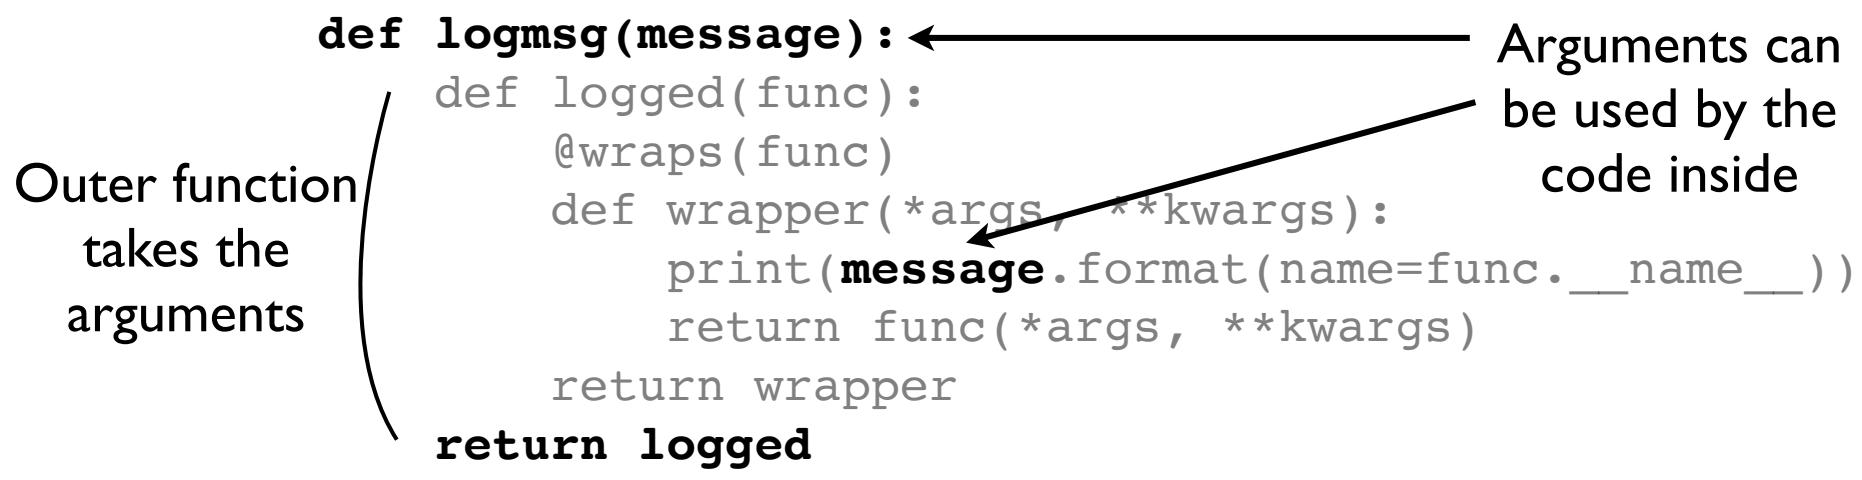
\includegraphics[keepaspectratio]{images/124286bd286128350453aadd439f648008def2cf0c6b5a189f5d34cc634df88b.jpg}}

The outer function is like an enclosing environment that gets added to
the decorator to accept the extra arguments

\bookmarksetup{startatroot}

\chapter{Decorators with Args}\label{decorators-with-args-3}

• Example: Logging with a custom message

def logmsg(message):

def logged(func):

The same decorator code as before

(\textbf{wraps?})(func)

def wrapper(*args, **kwargs):

print(message.format(name \(=\) func.\_\_name\_\_))

return func(*args, **kwargs)

return wrapper

return logged

Inner functions are standard decorator code

\bookmarksetup{startatroot}

\chapter{Decorators with Args}\label{decorators-with-args-4}

• Decorators with args are more general\\
• You can specialize to a no-argument case

logged \(=\) logmsg(`Calling \{name\}')

(\textbf{logged?})

def add(x, y):

return x + y

• This is subtle, but useful for simplifying code

\bookmarksetup{startatroot}

\chapter{Exercise 7.2}\label{exercise-7.2}

Time : 15 Minutes

\bookmarksetup{startatroot}

\chapter{Class Decorators}\label{class-decorators}

• Decorators can be applied to class definitions

\begin{Shaded}
\begin{Highlighting}[]
\NormalTok{@decorator   }
\NormalTok{class MyClass: def bar(self): def spam(self): }
\end{Highlighting}
\end{Shaded}

• It's exactly the same as doing this:

class MyClass: def bar(self): def spam(self): MyClass \(=\)
decorator``MyClass)

Manipulates or wraps a class

\bookmarksetup{startatroot}

\chapter{Class Decorators}\label{class-decorators-1}

Most class decorators inspect or do something special with the class
definition\\
Typical prototype

\begin{Shaded}
\begin{Highlighting}[]
\KeywordTok{def}\NormalTok{ decorator(cls):}
    \CommentTok{\# Do something with cls}
\NormalTok{    ...}
    \CommentTok{\# Return the original class back}
    \ControlFlowTok{return}\NormalTok{ cls }
\end{Highlighting}
\end{Shaded}

• Observe: The original class is not replaced

\bookmarksetup{startatroot}

\chapter{Example}\label{example-4}

\bookmarksetup{startatroot}

\chapter{Recording all attribute
lookups}\label{recording-all-attribute-lookups}

\begin{Shaded}
\begin{Highlighting}[]
\KeywordTok{def}\NormalTok{ logged\_getattr(cls):}
    \CommentTok{\# Get the original implementation}
\NormalTok{    orig\_getattribute }\OperatorTok{=}\NormalTok{ cls.}\FunctionTok{\_\_getattribute\_\_}
    \CommentTok{\# Replacement method}
    \KeywordTok{def} \FunctionTok{\_\_getattribute\_\_}\NormalTok{(}\VariableTok{self}\NormalTok{, name):}
        \BuiltInTok{print}\NormalTok{(}\StringTok{\textquotesingle{}Getting:\textquotesingle{}}\NormalTok{, name)}
        \ControlFlowTok{return}\NormalTok{ orig\_getattribute(}\VariableTok{self}\NormalTok{, name)}
    \CommentTok{\# Attach to the class}
\NormalTok{    cls.}\FunctionTok{\_\_getattribute\_\_} \OperatorTok{=} \FunctionTok{\_\_getattribute\_\_}
    \ControlFlowTok{return}\NormalTok{ cls }
\end{Highlighting}
\end{Shaded}

\bookmarksetup{startatroot}

\chapter{• This is replacing a method of the
class}\label{this-is-replacing-a-method-of-the-class}

\bookmarksetup{startatroot}

\chapter{Example}\label{example-5}

\begin{Shaded}
\begin{Highlighting}[]
\NormalTok{@logged\_getattr class MyClass: def foo(self): pass def bar(self): pass }
\end{Highlighting}
\end{Shaded}

\begin{quote}
\begin{quote}
\begin{quote}
s \(\equiv\) MyClass()\\
s.x \(= 23\) \textgreater\textgreater\textgreater s.x\\
Getting:x\\
s.foo()\\
Getting: foo\\
s.bar()\\
Getting: bar
\end{quote}
\end{quote}
\end{quote}

Notice how all lookups now have logging

\bookmarksetup{startatroot}

\chapter{Decoration via Inheritance}\label{decoration-via-inheritance}

• Base classes can observe inheritance

\begin{Shaded}
\begin{Highlighting}[]
\KeywordTok{class}\NormalTok{ Parent: }\OperatorTok{@}\NormalTok{classmethod }\KeywordTok{def} \FunctionTok{\_\_init\_subclass\_\_}\NormalTok{(cls, }\OperatorTok{**}\NormalTok{kwargs): }\CommentTok{\# Do something with cls (the subclass)   }
\KeywordTok{class}\NormalTok{ Child1(Parent): }\ControlFlowTok{pass}   
\KeywordTok{class}\NormalTok{ Child2(Parent, a}\OperatorTok{=}\DecValTok{1}\NormalTok{, b}\OperatorTok{=}\DecValTok{2}\NormalTok{): }\ControlFlowTok{pass} 
\end{Highlighting}
\end{Shaded}

• Makes it easier to have implicit class decorators

\bookmarksetup{startatroot}

\chapter{Exercise 7.3}\label{exercise-7.3}

Time : 15 Minutes

\bookmarksetup{startatroot}

\chapter{Disclaimer}\label{disclaimer}

• What follows is Python's most advanced bit\\
Took years for programmers to even understand what anyone was talking
about\\
Even now, the details are somewhat hairy\\
• Also known as the ``killer joke''

\bookmarksetup{startatroot}

\chapter{Types}\label{types}

As you hopefully know, all values in Python have an associated type\\
Example:

\begin{Shaded}
\begin{Highlighting}[]
\NormalTok{\textgreater{}\textgreater{}\textgreater{} x = 42  }
\NormalTok{\textgreater{}\textgreater{}\textgreater{} type(x)  }
\NormalTok{\textless{}class \textquotesingle{}int\textquotesingle{}\textgreater{}  }
\NormalTok{\textgreater{}\textgreater{}\textgreater{} s = \textquotesingle{}Hello\textquotesingle{}  }
\NormalTok{\textgreater{}\textgreater{}\textgreater{} type(s)  }
\NormalTok{\textless{}class \textquotesingle{}str\textquotesingle{}\textgreater{}  }
\NormalTok{\textgreater{}\textgreater{}\textgreater{} items = [1,2,3]  }
\NormalTok{\textgreater{}\textgreater{}\textgreater{} type(items)  }
\NormalTok{\textless{}class \textquotesingle{}list\textquotesingle{}\textgreater{}  }
\NormalTok{\textgreater{}\textgreater{}\textgreater{} }
\end{Highlighting}
\end{Shaded}

\bookmarksetup{startatroot}

\chapter{Type Constructor}\label{type-constructor}

The ``type'' is usually a callable for creating objects of that type\\
Example:

\begin{Shaded}
\begin{Highlighting}[]
\NormalTok{\textgreater{}\textgreater{}\textgreater{} items = [1,2,3]  }
\NormalTok{\textgreater{}\textgreater{}\textgreater{} type(item)  }
\NormalTok{\textless{}class \textquotesingle{}list\textquotesingle{}\textgreater{}  }
\NormalTok{\textgreater{}\textgreater{}\textgreater{} a = list()  \# Create a new list object  }
\NormalTok{\textgreater{}\textgreater{}\textgreater{} a  }
\NormalTok{[ ]  }
\NormalTok{\textgreater{}\textgreater{}\textgreater{} b = tuple(items)  \# Convert to a tuple }
\end{Highlighting}
\end{Shaded}

• Type conversions like this are common

\bookmarksetup{startatroot}

\chapter{Types and Classes}\label{types-and-classes}

• Classes also define new types

class Spam: pass\\
\textgreater\textgreater\textgreater s \(=\) Spam()\\
\textgreater\textgreater\textgreater type(s)\\
\textless class `main\textgreater.Spam'\textgreater{}\\
\textgreater\textgreater\textgreater{}

• It is exactly the same as with built-ins\\
• The class is the type of instances created\\
• The class is a callable that creates instances

\bookmarksetup{startatroot}

\chapter{Types of Classes}\label{types-of-classes}

• Classes are instances of types\\
• Observe by getting the type of a class itself

\begin{Shaded}
\begin{Highlighting}[]
\NormalTok{\textgreater{}\textgreater{}\textgreater{}class Spam:   }
\NormalTok{... pass   }
\NormalTok{\textgreater{}\textgreater{}\textgreater{}type(Spam)   }
\NormalTok{\textless{}class \textquotesingle{}type\textquotesingle{}\textgreater{}   }
\NormalTok{\textgreater{}\textgreater{}\textgreater{}isinstance(Spam,type)   }
\NormalTok{True   }
\NormalTok{\textgreater{}\textgreater{}\textgreater{} }
\end{Highlighting}
\end{Shaded}

Recall: type() tells you the type of an object. Here we're using it on a
class itself.

This requires some thought, but it should make some sense (a class is
simply a type)

\bookmarksetup{startatroot}

\chapter{Creating Types}\label{creating-types}

Head explosion: types are represented by their own class (type)

\begin{Shaded}
\begin{Highlighting}[]
\NormalTok{class type:}
\NormalTok{    ...}
\NormalTok{\textgreater{}\textgreater{}\textgreater{} type}
\NormalTok{\textless{}class \textquotesingle{}type\textquotesingle{}\textgreater{} }
\end{Highlighting}
\end{Shaded}

• This class creates new ``type'' objects\\
In fact, this is the class that processes class definitions when you
define your own classes

\bookmarksetup{startatroot}

\chapter{Classes Deconstructed}\label{classes-deconstructed}

\bookmarksetup{startatroot}

\chapter{Consider a class:}\label{consider-a-class}

\begin{Shaded}
\begin{Highlighting}[]
\KeywordTok{class}\NormalTok{ Spam(}\BuiltInTok{object}\NormalTok{): }\KeywordTok{def} \FunctionTok{\_\_init\_\_}\NormalTok{(}\VariableTok{self}\NormalTok{, name): }\VariableTok{self}\NormalTok{.name }\OperatorTok{=}\NormalTok{ name }\KeywordTok{def}\NormalTok{ yow(}\VariableTok{self}\NormalTok{): }\BuiltInTok{print}\NormalTok{(}\StringTok{"Yow! "}\NormalTok{, }\VariableTok{self}\NormalTok{.name) }
\end{Highlighting}
\end{Shaded}

\bookmarksetup{startatroot}

\chapter{What are its components?}\label{what-are-its-components}

Name (``Spam'')\\
• Base classes (object)\\
Functions (\textbf{init}, yow)

\bookmarksetup{startatroot}

\chapter{Creating a Class}\label{creating-a-class}

• You can create a class manually from pieces

\begin{Shaded}
\begin{Highlighting}[]
\NormalTok{Define some method functions }\KeywordTok{def} \FunctionTok{\_\_init\_\_}\NormalTok{(}\VariableTok{self}\NormalTok{, name): }\VariableTok{self}\NormalTok{.name }\OperatorTok{=}\NormalTok{ name }\KeywordTok{def}\NormalTok{ yow(}\VariableTok{self}\NormalTok{): }\BuiltInTok{print}\NormalTok{(}\StringTok{"Yow!"}\NormalTok{, }\VariableTok{self}\NormalTok{.name) }
\end{Highlighting}
\end{Shaded}

Make a method table methods \(=\) \{`init': init, `yow': yow\}

\begin{Shaded}
\begin{Highlighting}[]
\NormalTok{Make a new type (Spam)  }
\NormalTok{Spam = type(\textquotesingle{}Spam\textquotesingle{}, (object), methods) }
\end{Highlighting}
\end{Shaded}

• These steps mimic the class statement

\bookmarksetup{startatroot}

\chapter{Class Definition Process}\label{class-definition-process}

• What happens during class definition?

\begin{Shaded}
\begin{Highlighting}[]
\KeywordTok{class}\NormalTok{ Spam(}\BuiltInTok{object}\NormalTok{): }\KeywordTok{def} \FunctionTok{\_\_init\_\_}\NormalTok{(}\VariableTok{self}\NormalTok{, name): }\VariableTok{self}\NormalTok{.name }\OperatorTok{=}\NormalTok{ name }\KeywordTok{def}\NormalTok{ yow(}\VariableTok{self}\NormalTok{): }\BuiltInTok{print}\NormalTok{(}\StringTok{"Yow! "}\NormalTok{, }\VariableTok{self}\NormalTok{.name) }
\end{Highlighting}
\end{Shaded}

Step1: Body of class is captured

body \(=\) def init\_self, name): self.name \(\equiv\) name def
yow(self): print(``Yow!'', self.name)

\bookmarksetup{startatroot}

\chapter{Class Definition Process}\label{class-definition-process-1}

• Step 2: A dictionary is created

\textbf{dict} = type.\_\_prepare\_\_(`Spam', (object,))

• Normally, you get a plain Python dictionary

\begin{Shaded}
\begin{Highlighting}[]
\NormalTok{\textgreater{}\textgreater{}\textgreater{} type}\KeywordTok{.}\DataTypeTok{\_prepare\_\_}\NormalTok{(}\ErrorTok{‘}\DataTypeTok{Spam}\StringTok{\textquotesingle{}}\ErrorTok{, (object,)  }
\ErrorTok{\{\}  }
\ErrorTok{\textgreater{}\textgreater{}\textgreater{} }
\end{Highlighting}
\end{Shaded}

Some extra metadata is inserted

\begin{Shaded}
\begin{Highlighting}[]
\NormalTok{\_\_dict\_\_[}\StringTok{\textquotesingle{}\_\_qualname\_\_\textquotesingle{}}\NormalTok{] }\OperatorTok{=} \StringTok{\textquotesingle{}Spam\textquotesingle{}}  
\NormalTok{\_\_dict\_\_[}\StringTok{\textquotesingle{}\_\_module\_\_\textquotesingle{}}\NormalTok{] }\OperatorTok{=} \StringTok{\textquotesingle{}modulo\textquotesingle{}} 
\end{Highlighting}
\end{Shaded}

\bookmarksetup{startatroot}

\chapter{Class Definition Process}\label{class-definition-process-2}

• Step 3: Class body is executed in the dict

exec(body, globals(), \textbf{dict})

• The statements in the body run like a script\\
• Afterwards, \textbf{dict} is populated

\begin{Shaded}
\begin{Highlighting}[]
\NormalTok{\textgreater{}\textgreater{}\textgreater{} \_dict\_  }
\NormalTok{\{  }
\NormalTok{    \textquotesingle{}\_\_init\_\_\textquotesingle{}: \textless{}function \_\_init\_\_ at 0x4da10\textgreater{},  }
\NormalTok{    \textquotesingle{}yow\textquotesingle{}: \textless{}function yow at 0x4dd70\textgreater{}\},  }
\NormalTok{    \textquotesingle{}\_\_qualname\_\_\textquotesingle{}: \textquotesingle{}Spam\textquotesingle{},  }
\NormalTok{    \textquotesingle{}\_\_module\_\_\textquotesingle{}: \textquotesingle{}modulename\textquotesingle{}  }
\NormalTok{\}  }
\NormalTok{\textgreater{}\textgreater{}\textgreater{} }
\end{Highlighting}
\end{Shaded}

\bookmarksetup{startatroot}

\chapter{Class Definition Process}\label{class-definition-process-3}

Step 4: Class is constructed from its name, base classes, and the
dictionary

\begin{Shaded}
\begin{Highlighting}[]
\NormalTok{\textgreater{}\textgreater{}\textgreater{} Spam = type(\textquotesingle{}Spam\textquotesingle{}, (object), \_\_dict\_\_)  }
\NormalTok{\textgreater{}\textgreater{}\textgreater{} Spam  }
\NormalTok{\textless{}class\_\_main\_\_.Spam\textquotesingle{}\textgreater{}  }
\NormalTok{\textgreater{}\textgreater{}\textgreater{} s = Spam(\textquotesingle{}Guido\textquotesingle{})  }
\NormalTok{\textgreater{}\textgreater{}\textgreater{} s.yow()  }
\NormalTok{Yow! Guido  }
\NormalTok{\textgreater{}\textgreater{}\textgreater{} }
\end{Highlighting}
\end{Shaded}

type(name, bases, dict) constructs a class object

\bookmarksetup{startatroot}

\chapter{Exercise 7.4}\label{exercise-7.4}

Time : 15 Minutes

\bookmarksetup{startatroot}

\chapter{Metaclasses Defined}\label{metaclasses-defined}

• A class that creates classes is called a metaclass\\
type is an example of a metaclass

\bookmarksetup{startatroot}

\chapter{The Metaclass Hook}\label{the-metaclass-hook}

Python provides a hook that allows you to override the class creation
steps\\
You can use a different metaclass than ``type''\\
Using this, you can completely customize what happens when a class is
created.

\bookmarksetup{startatroot}

\chapter{Metaclass Selection}\label{metaclass-selection}

metaclass keyword argument\\
• Sets the class used to create the class object

\begin{Shaded}
\begin{Highlighting}[]
\KeywordTok{class}\NormalTok{ Spam(metaclass}\OperatorTok{=}\BuiltInTok{type}\NormalTok{): }\KeywordTok{def} \FunctionTok{\_\_init\_\_}\NormalTok{(}\VariableTok{self}\NormalTok{, name): }\VariableTok{self}\NormalTok{.name }\OperatorTok{=}\NormalTok{ name }\KeywordTok{def}\NormalTok{ yow(}\VariableTok{self}\NormalTok{): }\BuiltInTok{print}\NormalTok{(}\StringTok{"Yow! "}\NormalTok{, }\VariableTok{self}\NormalTok{.name) }
\end{Highlighting}
\end{Shaded}

By default, it's set to `type', but you change it to something else
(more shortly)

\bookmarksetup{startatroot}

\chapter{Metaclass Selection}\label{metaclass-selection-1}

Compatibility note: Python 2 is different\\
• Use the \textbf{metaclass} attribute instead

\begin{Shaded}
\begin{Highlighting}[]
\KeywordTok{class}\NormalTok{ Spam: \_\_metaclass\_\_ }\OperatorTok{=} \BuiltInTok{type} \CommentTok{\# Python 2 only}
\KeywordTok{def} \FunctionTok{\_\_init\_\_}\NormalTok{(}\VariableTok{self}\NormalTok{, name):}
    \VariableTok{self}\NormalTok{.name }\OperatorTok{=}\NormalTok{ name}
\KeywordTok{def}\NormalTok{ yow(}\VariableTok{self}\NormalTok{):}
    \BuiltInTok{print}\NormalTok{(}\StringTok{"Yow!"}\NormalTok{, }\VariableTok{self}\NormalTok{.name) }
\end{Highlighting}
\end{Shaded}

Comment: Very difficult to provide Py2/3 compatibility due to syntax
difference

\bookmarksetup{startatroot}

\chapter{Metaclass Inheritance}\label{metaclass-inheritance}

If no metaclass is set, Python uses the same type as the base class

\begin{Shaded}
\begin{Highlighting}[]
\KeywordTok{class}\NormalTok{ Spam(}\BuiltInTok{object}\NormalTok{): }\KeywordTok{def} \FunctionTok{\_\_init\_\_}\NormalTok{(}\VariableTok{self}\NormalTok{, name): }\VariableTok{self}\NormalTok{.name }\OperatorTok{=}\NormalTok{ name }\KeywordTok{def}\NormalTok{ yow(}\VariableTok{self}\NormalTok{): }\BuiltInTok{print}\NormalTok{(}\StringTok{"Yow!"}\NormalTok{) }\OperatorTok{\textgreater{}\textgreater{}\textgreater{}} \BuiltInTok{object}\NormalTok{.\_class\_ }\OperatorTok{\textless{}}\KeywordTok{class} \StringTok{\textquotesingle{}type\textquotesingle{}}\OperatorTok{\textgreater{}} \OperatorTok{\textgreater{}\textgreater{}\textgreater{}} \BuiltInTok{type}\NormalTok{(Foo) }\OperatorTok{\textless{}}\KeywordTok{class} \StringTok{\textquotesingle{}type\textquotesingle{}}\OperatorTok{\textgreater{}} 
\end{Highlighting}
\end{Shaded}

Note: this is why you rarely see it

\bookmarksetup{startatroot}

\chapter{Creating a New Metaclass}\label{creating-a-new-metaclass}

• You inherit from type and redefine methods such as \textbf{new},
\textbf{prepare}, etc.

\begin{Shaded}
\begin{Highlighting}[]
\KeywordTok{class}\NormalTok{ mytype(}\BuiltInTok{type}\NormalTok{):}
    \AttributeTok{@staticmethod}
    \KeywordTok{def} \FunctionTok{\_\_new\_\_}\NormalTok{(meta, name, bases, methods):}
        \BuiltInTok{print}\NormalTok{(}\StringTok{\textquotesingle{}Creating class: \textquotesingle{}}\NormalTok{, name)}
        \BuiltInTok{print}\NormalTok{(}\StringTok{\textquotesingle{}Base classes: \textquotesingle{}}\NormalTok{, bases)}
        \BuiltInTok{print}\NormalTok{(}\StringTok{\textquotesingle{}Attributes: \textquotesingle{}}\NormalTok{, }\BuiltInTok{list}\NormalTok{(methods))}
    \ControlFlowTok{return} \BuiltInTok{super}\NormalTok{().}\FunctionTok{\_\_new\_\_}\NormalTok{(meta, name, bases, methods) }
\end{Highlighting}
\end{Shaded}

• Then you define a new root-object

class myobject(metaclass=mytype): pass

\bookmarksetup{startatroot}

\chapter{Using a Metaclass}\label{using-a-metaclass}

• To use the new metaclass, define classes so that they inherit from
your root object

\begin{Shaded}
\begin{Highlighting}[]
\KeywordTok{class}\NormalTok{ Spam(myobject):}
    \KeywordTok{def} \FunctionTok{\_\_init\_\_}\NormalTok{(}\VariableTok{self}\NormalTok{, name):}
        \VariableTok{self}\NormalTok{.name }\OperatorTok{=}\NormalTok{ name}
    \KeywordTok{def}\NormalTok{ yow(}\VariableTok{self}\NormalTok{):}
        \BuiltInTok{print}\NormalTok{(}\StringTok{"Yow!"}\NormalTok{, }\VariableTok{self}\NormalTok{.name) }
\end{Highlighting}
\end{Shaded}

• You should see your metaclass at work

\begin{Shaded}
\begin{Highlighting}[]
\NormalTok{Creating class : Spam  }
\NormalTok{Base classes : (\textless{}class \textquotesingle{}\_\_main\_\_.myobject\textquotesingle{}\textgreater{},)  }
\NormalTok{Attributes : [\textquotesingle{}yow\textquotesingle{}, \textquotesingle{}\_\_module\_\_\textquotesingle{}, \textquotesingle{}\_\_init\_\_\textquotesingle{}] }
\end{Highlighting}
\end{Shaded}

\bookmarksetup{startatroot}

\chapter{Exercise 7.5}\label{exercise-7.5}

Time : 10 Minutes

\bookmarksetup{startatroot}

\chapter{Typical Applications}\label{typical-applications}

Metaclasses allow alteration of the class definition process itself\\
• Setting up the class definition environment\\
Changing instance creation\\
Coding conventions/rules

\bookmarksetup{startatroot}

\chapter{Using a Metaclass}\label{using-a-metaclass-1}

Metaclasses allow class definitions to be monitored and manipulated\\
• There are 4 main interception points

\begin{Shaded}
\begin{Highlighting}[]
\BuiltInTok{type}\NormalTok{.\_prepare\_\_(name, bases)  }
\BuiltInTok{type}\NormalTok{.\_new\_\_(}\BuiltInTok{type}\NormalTok{, name, bases, }\BuiltInTok{dict}\NormalTok{)  }
\BuiltInTok{type}\NormalTok{.\_init\_\_(cls, name, bases, }\BuiltInTok{dict}\NormalTok{) }
\end{Highlighting}
\end{Shaded}

class definition

type.\_\_call\_\_(cls, *args, **kwargs)

instance creation

\bookmarksetup{startatroot}

\chapter{Example: Duplicate Check}\label{example-duplicate-check}

class dupedict(dict): def \textbf{setitem}(self, key, value): assert key
not in self, `\%s duplicated' \% key super().\_\_setitem\_\_(key, value)

class dupemeta(type): (\textbf{classmethod?}) def \textbf{prepare}(cls,
name, bases): return dupedict()

Example:

class A(metaclass \(=\) dupemeta): def bar(self): pass def
bar(self):pass Fails! Duplicate

\bookmarksetup{startatroot}

\chapter{Example: Decoration}\label{example-decoration}

def decorator(func):

\begin{Shaded}
\begin{Highlighting}[]
\NormalTok{...   }
\NormalTok{\# Decorator   }
\NormalTok{. }
\end{Highlighting}
\end{Shaded}

\begin{Shaded}
\begin{Highlighting}[]
\KeywordTok{class}\NormalTok{ meta(}\BuiltInTok{type}\NormalTok{):}
    \AttributeTok{@staticmethod}
    \KeywordTok{def} \FunctionTok{\_\_new\_\_}\NormalTok{(meta, clsname, bases, }\BuiltInTok{dict}\NormalTok{):}
        \ControlFlowTok{for}\NormalTok{ key, val }\KeywordTok{in} \BuiltInTok{dict}\NormalTok{.items():}
            \ControlFlowTok{if} \BuiltInTok{callable}\NormalTok{(val):}
                \BuiltInTok{dict}\NormalTok{[key] }\OperatorTok{=}\NormalTok{ decorator(val)}
            \ControlFlowTok{return} \BuiltInTok{super}\NormalTok{().}\FunctionTok{\_\_new\_\_}\NormalTok{(meta, clsname, bases, }\BuiltInTok{dict}\NormalTok{) }
\end{Highlighting}
\end{Shaded}

• This class wraps all methods with a decorator

\bookmarksetup{startatroot}

\chapter{Example: Instance Creation}\label{example-instance-creation}

\begin{Shaded}
\begin{Highlighting}[]
\KeywordTok{class}\NormalTok{ meta(}\BuiltInTok{type}\NormalTok{): }\KeywordTok{def} \FunctionTok{\_\_call\_\_}\NormalTok{(cls, }\OperatorTok{*}\NormalTok{args, }\OperatorTok{**}\NormalTok{kwargs): }\BuiltInTok{print}\NormalTok{(}\StringTok{\textquotesingle{}Creating instance of\textquotesingle{}}\NormalTok{, cls) }\ControlFlowTok{return} \BuiltInTok{super}\NormalTok{().}\FunctionTok{\_\_call\_\_}\NormalTok{((}\OperatorTok{*}\NormalTok{args, }\OperatorTok{**}\NormalTok{kwargs) }
\end{Highlighting}
\end{Shaded}

Example:

\begin{Shaded}
\begin{Highlighting}[]
\NormalTok{\textgreater{}\textgreater{}\textgreater{} class A(metaclass=meta): pass }
\end{Highlighting}
\end{Shaded}

\begin{Shaded}
\begin{Highlighting}[]
\NormalTok{\textgreater{}\textgreater{}\textgreater{} a = A()}
\NormalTok{Creating instance of \textless{}class \textquotesingle{}\_\_main\_\_.A\textquotesingle{}\textgreater{} }
\end{Highlighting}
\end{Shaded}

Potentially useful for special cases (singletons, caching, etc.)

\bookmarksetup{startatroot}

\chapter{Commentary}\label{commentary-4}

Metaclasses are not something you should be defining without really good
reasons\\
Target audience:

Framework builders\\
Library developers

Consider using a class decorator first\\
End users should not be messing around with metaclasses in their own
code

\bookmarksetup{startatroot}

\chapter{Exercise 7.6}\label{exercise-7.6}

Time : 10 Minutes

\bookmarksetup{startatroot}

\chapter{Section 8}\label{section-8}

\bookmarksetup{startatroot}

\chapter{Iterators, Generators, and
Coroutines}\label{iterators-generators-and-coroutines}

\bookmarksetup{startatroot}

\chapter{Iteration}\label{iteration-1}

Iteration defined: Looping over items

\[
a = [ 2, 4, 1 0, 3 7, 6 2 ]
\]

\bookmarksetup{startatroot}

\chapter{Iterate over a}\label{iterate-over-a}

for x in a:

• A very common pattern\\
• loops, list comprehensions, etc.\\
• Most programs do a huge amount of iteration

\bookmarksetup{startatroot}

\chapter{Iteration: Protocol}\label{iteration-protocol}

\bookmarksetup{startatroot}

\chapter{Iteration}\label{iteration-2}

for x in obj: \# statements

\bookmarksetup{startatroot}

\chapter{Underneath the covers}\label{underneath-the-covers}

\_\_iter = obj.\_\_iter\_\_( ) \# Get iterator object while True: try:
\(\mathbf{x} =\) \emph{iter.\_next}( \#Get next item except
StopIteration: \#No more items break \#statements

\bookmarksetup{startatroot}

\chapter{Objects that work with the for-loop all implement this
low-level iteration
protocol}\label{objects-that-work-with-the-for-loop-all-implement-this-low-level-iteration-protocol}

\bookmarksetup{startatroot}

\chapter{Iteration: Protocol}\label{iteration-protocol-1}

\bookmarksetup{startatroot}

\chapter{Example: Manual iteration over a
list}\label{example-manual-iteration-over-a-list}

\begin{Shaded}
\begin{Highlighting}[]
\NormalTok{\textgreater{}\textgreater{}\textgreater{} x = [1,2,3]  }
\NormalTok{\textgreater{}\textgreater{}\textgreater{} it = x.\_\_iter\_\_(  )  }
\NormalTok{\textgreater{}\textgreater{}\textgreater{} it  }
\NormalTok{\textless{}順次iterator object at 0x590b0\textgreater{}  }
\NormalTok{\textgreater{}\textgreater{}\textgreater{} it.\_next\_\_()  }
\NormalTok{1  }
\NormalTok{\textgreater{}\textgreater{}\textgreater{} it.\_next\_\_()  }
\NormalTok{2  }
\NormalTok{\textgreater{}\textgreater{}\textgreater{} it.\_next\_\_()  }
\NormalTok{3  }
\NormalTok{\textgreater{}\textgreater{}\textgreater{} it.\_next\_\_()  }
\NormalTok{Traceback (most recent call last):  }
\NormalTok{    File "\textless{}stdin\textgreater{}", line 1, in ?  }
\NormalTok{StopIteration  }
\NormalTok{\textgreater{}\textgreater{}\textgreater{} }
\end{Highlighting}
\end{Shaded}

\bookmarksetup{startatroot}

\chapter{Delegating Iteration}\label{delegating-iteration}

• Sometimes custom containers will delegate

\begin{Shaded}
\begin{Highlighting}[]
\KeywordTok{class}\NormalTok{ Portfolio: }\KeywordTok{def} \FunctionTok{\_\_init\_\_}\NormalTok{(}\VariableTok{self}\NormalTok{): }\VariableTok{self}\NormalTok{.\_holdings }\OperatorTok{=}\NormalTok{ [] }\KeywordTok{def} \FunctionTok{\_\_iter\_\_}\NormalTok{(}\VariableTok{self}\NormalTok{): }\ControlFlowTok{return} \VariableTok{self}\NormalTok{.\_holdings.\_iter\_() }
\end{Highlighting}
\end{Shaded}

• Making containers iterable usually a good idea

\bookmarksetup{startatroot}

\chapter{Generators}\label{generators-1}

\bookmarksetup{startatroot}

\chapter{Generators simplify customized
iteration}\label{generators-simplify-customized-iteration}

\begin{Shaded}
\begin{Highlighting}[]
\KeywordTok{def}\NormalTok{ countdown(n):}
    \BuiltInTok{print}\NormalTok{(}\StringTok{\textquotesingle{}Counting down from\textquotesingle{}}\NormalTok{, n)}
    \ControlFlowTok{while}\NormalTok{ n }\OperatorTok{\textgreater{}} \DecValTok{0}\NormalTok{:}
        \ControlFlowTok{yield}\NormalTok{ n}
\NormalTok{        n }\OperatorTok{{-}=} \DecValTok{1} 
\end{Highlighting}
\end{Shaded}

\begin{Shaded}
\begin{Highlighting}[]
\NormalTok{\textgreater{}\textgreater{}\textgreater{} for i in countdown(5): print(\textquotesingle{}T{-}minus\textquotesingle{}, i)   }
\NormalTok{Counting down from 5   }
\NormalTok{T{-}minus 5   }
\NormalTok{T{-}minus 4   }
\NormalTok{T{-}minus 3   }
\NormalTok{T{-}minus 2   }
\NormalTok{T{-}minus 1   }
\NormalTok{\textgreater{}\textgreater{}\textgreater{} }
\end{Highlighting}
\end{Shaded}

\bookmarksetup{startatroot}

\chapter{Generator Functions}\label{generator-functions-1}

• Behavior is different than normal func\\
• Calling a generator function creates an generator object. It does not
start running the function.

\begin{Shaded}
\begin{Highlighting}[]
\KeywordTok{def}\NormalTok{ countdown(n):}
    \BuiltInTok{print}\NormalTok{(}\StringTok{\textquotesingle{}Counting down from\textquotesingle{}}\NormalTok{, n)}
    \ControlFlowTok{while}\NormalTok{ n }\OperatorTok{\textgreater{}} \DecValTok{0}\NormalTok{:}
        \ControlFlowTok{yield}\NormalTok{ n}
\NormalTok{        n }\OperatorTok{{-}=} \DecValTok{1}
\OperatorTok{\textgreater{}\textgreater{}\textgreater{}}\NormalTok{ x }\OperatorTok{=}\NormalTok{ countdown(}\DecValTok{10}\NormalTok{) }\OperatorTok{\textless{}}\NormalTok{ Notice that no output was produced}
\OperatorTok{\textgreater{}\textgreater{}\textgreater{}}\NormalTok{ x}
\OperatorTok{\textless{}}\NormalTok{generator }\BuiltInTok{object}\NormalTok{ at }\BaseNTok{0x58490}\OperatorTok{\textgreater{}}
\OperatorTok{\textgreater{}\textgreater{}\textgreater{}} 
\end{Highlighting}
\end{Shaded}

\bookmarksetup{startatroot}

\chapter{Generator Functions}\label{generator-functions-2}

• Function only executes on next()

\begin{Shaded}
\begin{Highlighting}[]
\NormalTok{\textgreater{}\textgreater{}\textgreater{} x = countdown(10)  }
\NormalTok{\textgreater{}\textgreater{}\textgreater{} x  }
\NormalTok{\textless{}generator object at 0x58490\textgreater{}  }
\NormalTok{\textgreater{}\textgreater{}\textgreater{} next(x) \# invokes x.\_next\_()  }
\NormalTok{Counting down from 10  }
\NormalTok{Function starts  }
\NormalTok{10 executing here }
\end{Highlighting}
\end{Shaded}

yield produces a value, but suspends function\\
Function resumes on next call to next()

\begin{Shaded}
\begin{Highlighting}[]
\NormalTok{\textgreater{}\textgreater{}\textgreater{} next(x)   }
\NormalTok{9   }
\NormalTok{\textgreater{}\textgreater{}\textgreater{} next(x)   }
\NormalTok{8   }
\NormalTok{\textgreater{}\textgreater{}\textgreater{} }
\end{Highlighting}
\end{Shaded}

\bookmarksetup{startatroot}

\chapter{Generator Functions}\label{generator-functions-3}

• When the generator returns, iteration stops

\begin{Shaded}
\begin{Highlighting}[]
\OperatorTok{\textgreater{}\textgreater{}\textgreater{}} \FunctionTok{next(}\CharTok{x}\FunctionTok{)}   
\DecValTok{1}   
\OperatorTok{\textgreater{}\textgreater{}\textgreater{}}\FunctionTok{next(}\CharTok{x}\FunctionTok{)}   
\VariableTok{Traceback} \FunctionTok{(}\CharTok{most} \CharTok{recent} \CharTok{call} \CharTok{last}\FunctionTok{):} \VariableTok{File} \StringTok{"\textless{}stdin\textgreater{}"}\FunctionTok{,} \CharTok{line} \DecValTok{1}\FunctionTok{,} \CharTok{in} \FunctionTok{?}   
\VariableTok{StopIteration}   
\OperatorTok{\textgreater{}\textgreater{}\textgreater{}} 
\end{Highlighting}
\end{Shaded}

Observation : A generator function implements the same low-level
protocol that the for statement uses on lists, tuples, dicts, files,
etc.

\bookmarksetup{startatroot}

\chapter{Reusing Generators}\label{reusing-generators}

\bookmarksetup{startatroot}

\chapter{Generators are one-time use}\label{generators-are-one-time-use}

\begin{Shaded}
\begin{Highlighting}[]
\NormalTok{\textgreater{}\textgreater{}\textgreater{} c = countdown(5)  }
\NormalTok{\textgreater{}\textgreater{}\textgreater{} for x in c:  }
\NormalTok{... print(\textquotesingle{}T{-}minus\textquotesingle{}, x)  }
\NormalTok{...  }
\NormalTok{T{-}minus 5  }
\NormalTok{T{-}minus 4  }
\NormalTok{T{-}minus 3  }
\NormalTok{T{-}minus 2  }
\NormalTok{T{-}minus 1  }
\NormalTok{\textgreater{}\textgreater{}\textgreater{} for x in c:  }
\NormalTok{... print(\textquotesingle{}T{-}minus\textquotesingle{}, x)  }
\NormalTok{...  }
\NormalTok{\textgreater{}\textgreater{}\textgreater{} }
\end{Highlighting}
\end{Shaded}

\bookmarksetup{startatroot}

\chapter{• You can recreate to start
again}\label{you-can-recreate-to-start-again}

\begin{Shaded}
\begin{Highlighting}[]
\OperatorTok{\textgreater{}\textgreater{}\textgreater{}}\NormalTok{ c }\OperatorTok{=}\NormalTok{ countdown(}\DecValTok{5}\NormalTok{) }
\end{Highlighting}
\end{Shaded}

\bookmarksetup{startatroot}

\chapter{Reusable Generators}\label{reusable-generators}

• Subtle trick: Make a class with \textbf{iter}()

class Countdown:

\begin{Shaded}
\begin{Highlighting}[]
\KeywordTok{def} \FunctionTok{\_\_init\_\_}\NormalTok{(}\VariableTok{self}\NormalTok{, n):}
    \VariableTok{self}\NormalTok{.n }\OperatorTok{=}\NormalTok{ n }
\end{Highlighting}
\end{Shaded}

\begin{Shaded}
\begin{Highlighting}[]
\KeywordTok{def} \FunctionTok{\_\_iter\_\_}\NormalTok{(}\VariableTok{self}\NormalTok{):}
\NormalTok{    n }\OperatorTok{=} \VariableTok{self}\NormalTok{.n}
\ControlFlowTok{while}\NormalTok{ n }\OperatorTok{\textgreater{}} \DecValTok{0}\NormalTok{:}
    \ControlFlowTok{yield}\NormalTok{ n}
\NormalTok{    n }\OperatorTok{{-}=} \DecValTok{1} 
\end{Highlighting}
\end{Shaded}

• Every use of iteration makes a new generator

\bookmarksetup{startatroot}

\chapter{Exercise 8.}\label{exercise-8.}

Time : 20 Minutes

\bookmarksetup{startatroot}

\chapter{Producers \& Consumers}\label{producers-consumers}

Generators are closely related to various forms of ``producer-consumer''
programming

producer

\pandocbounded{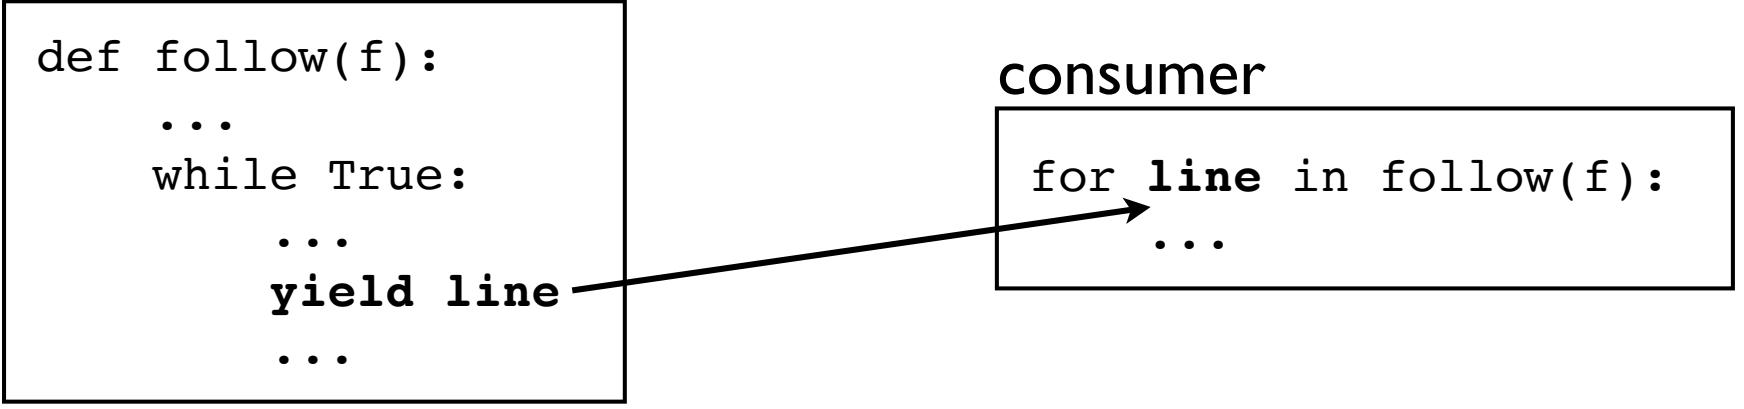
\includegraphics[keepaspectratio]{images/a77fe657bde54782b3486432744db8c2e69df5186fed94436e517444f6d57e07.jpg}}

yield produces values\\
for consume values

\bookmarksetup{startatroot}

\chapter{Generator Pipelines}\label{generator-pipelines}

You can use this aspect of generators to set up processing pipelines
(like Unix pipes)\\
Big picture:

\pandocbounded{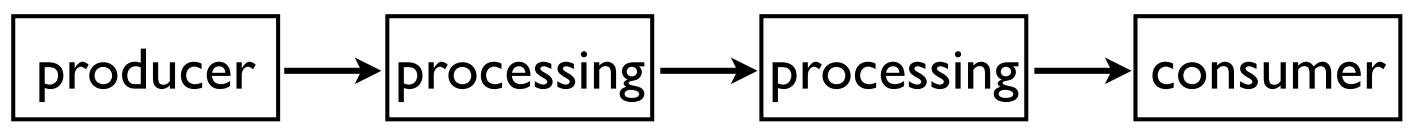
\includegraphics[keepaspectratio]{images/13083694888351a8f0ecca9dda10d2b25926e7d07205bfe3effe8a6aa61fcdf3.jpg}}

Processing pipes have an initial data producer, some set of intermediate
processing stages, and a final consumer

\bookmarksetup{startatroot}

\chapter{Generator Pipelines}\label{generator-pipelines-1}

\pandocbounded{
\includegraphics[keepaspectratio]{images/00dfa991a1e03f07031e62b65d0072b4d09c39a1e79438333960bc902d22d0bb.jpg}}

def producer():

yield item

Producer is typically a generator (although it could also be a list or
some other sequence)\\
yield feeds data into the pipeline

\bookmarksetup{startatroot}

\chapter{Generator Pipelines}\label{generator-pipelines-2}

\pandocbounded{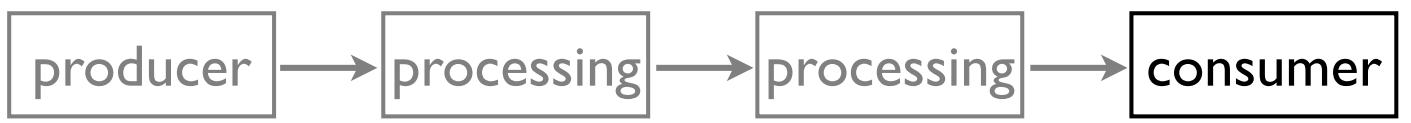
\includegraphics[keepaspectratio]{images/0f547f45abfdd35f27a9990ee447db5fc536c86fe3f0e5df1507ab8b3a7d99f5.jpg}}

def producer():

yield item

def consumer(s):

for item in s:

Consumer is just a simple for-loop\\
• It gets items and does something with them

\bookmarksetup{startatroot}

\chapter{Generator Pipelines}\label{generator-pipelines-3}

\pandocbounded{
\includegraphics[keepaspectratio]{images/64414166363e3ce537f5c5de2d3d0ae34c2c0480a45de74b343b547a24bc9c6e.jpg}}

def producer():

yield item

def processing(s):

for item in s:

yield newitem

def consumer(s):

for item in s:

Intermediate processing stages simultaneously consume and produce
items\\
• They might modify the data stream\\
• They can also filter (discarding items)

\bookmarksetup{startatroot}

\chapter{Generator Pipelines}\label{generator-pipelines-4}

\pandocbounded{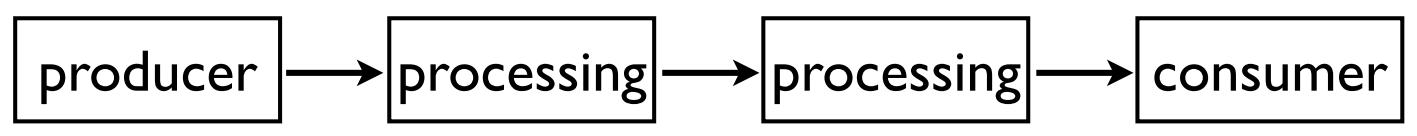
\includegraphics[keepaspectratio]{images/fe89171bbd6fedf37d2c1ad91a29d112e5e796459daaa2a9a071bae3e194b317.jpg}}

\pandocbounded{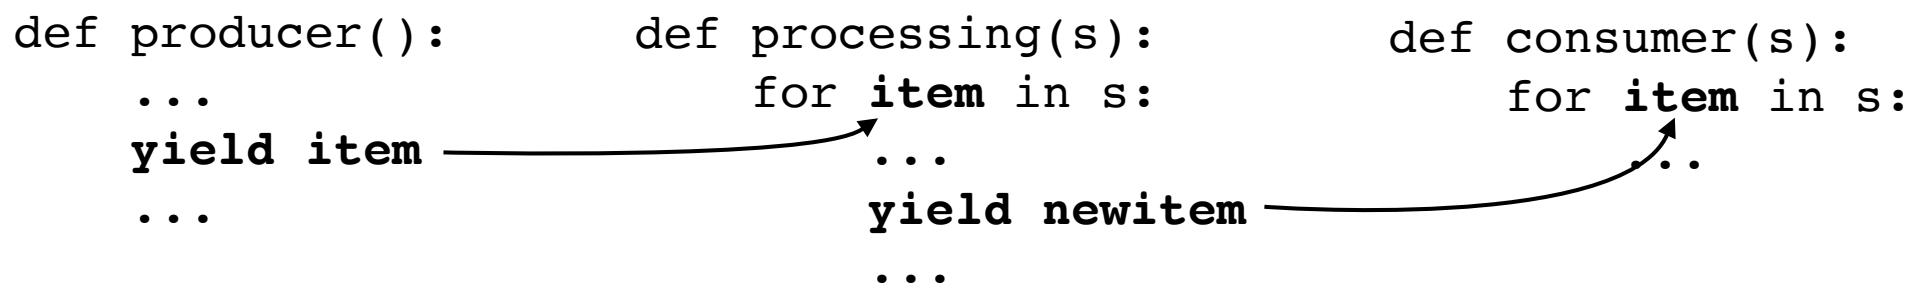
\includegraphics[keepaspectratio]{images/01641afe5f78742d01604d37a69081f3d1aec2fb67f2a662aba128c18f658304.jpg}}

Pipeline setup (in your program)

\pandocbounded{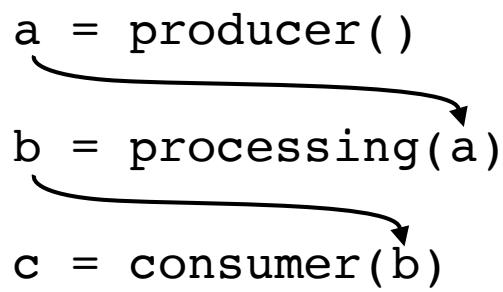
\includegraphics[keepaspectratio]{images/89eb23a6ab662d835f6d6c13bd8972304f81afb43ce7c62173bb671d8400334e.jpg}}

You will notice that data incrementally flows through the different
functions

\bookmarksetup{startatroot}

\chapter{Exercise 8.2}\label{exercise-8.2}

Time : 15 minutes

\bookmarksetup{startatroot}

\chapter{Yield as an Expression}\label{yield-as-an-expression}

• In generators, yield can be used as an expression\\
• For example, on the right side of an assignment

\begin{Shaded}
\begin{Highlighting}[]
\KeywordTok{def}\NormalTok{ match(pattern):}
    \BuiltInTok{print}\NormalTok{(}\StringTok{\textquotesingle{}Looking for }\SpecialCharTok{\%s}\StringTok{\textquotesingle{}} \OperatorTok{\%}\NormalTok{ pattern)}
\ControlFlowTok{while} \VariableTok{True}\NormalTok{:}
\NormalTok{    line }\OperatorTok{=} \ControlFlowTok{yield}
    \ControlFlowTok{if}\NormalTok{ pattern }\KeywordTok{in}\NormalTok{ line:}
        \BuiltInTok{print}\NormalTok{(line) }
\end{Highlighting}
\end{Shaded}

Question : What is its value?

\bookmarksetup{startatroot}

\chapter{Coroutines}\label{coroutines}

• If you use yield like this, you get a ``coroutine''\\
• It defines a function to which you send values

\begin{Shaded}
\begin{Highlighting}[]
\NormalTok{\textgreater{}\textgreater{}\textgreater{} g = match(\textquotesingle{}python\textquotesingle{})}
\NormalTok{\textgreater{}\textgreater{}\textgreater{} g.send(None) \# Prime it (explained shortly)}
\NormalTok{Looking for python}
\NormalTok{\textgreater{}\textgreater{}\textgreater{} g.send(\textquotesingle{}Yeah, but no, but yeah, but no\textquotesingle{})}
\NormalTok{\textgreater{}\textgreater{}\textgreater{} g.send(\textquotesingle{}A series of tubes\textquotesingle{})}
\NormalTok{\textgreater{}\textgreater{}\textgreater{} g.send(\textquotesingle{}python generators rock!\textquotesingle{})}
\NormalTok{python generators rock!}
\NormalTok{\textgreater{}\textgreater{}\textgreater{} }
\end{Highlighting}
\end{Shaded}

Sent values are returned by (yield)

\bookmarksetup{startatroot}

\chapter{Coroutine Execution}\label{coroutine-execution}

Execution is the same as for a generator\\
• When you call a coroutine, nothing happens\\
• Only runs in response to send() method

\pandocbounded{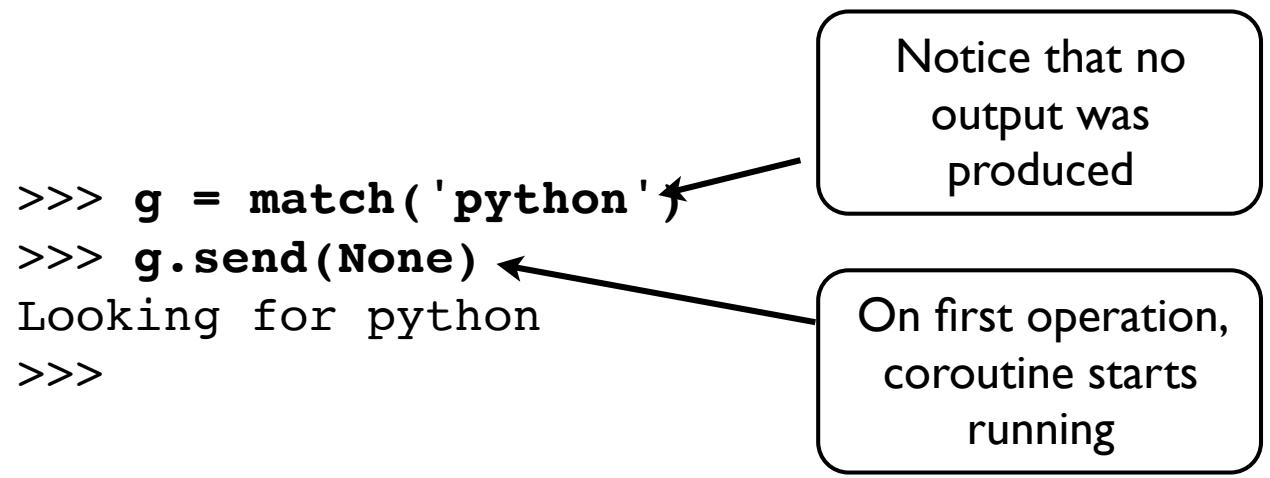
\includegraphics[keepaspectratio]{images/87998a83493bbcb697b9afc3620c7017911e9bdfd186e0576cd0586e5baa5fa8.jpg}}

\bookmarksetup{startatroot}

\chapter{Coroutine Priming}\label{coroutine-priming}

• All coroutines must be ``primed'' by first calling send(None)\\
This advances execution to the location of the first yield expression.

\begin{Shaded}
\begin{Highlighting}[]
\KeywordTok{def}\NormalTok{ match(pattern):}
    \BuiltInTok{print}\NormalTok{(}\StringTok{\textquotesingle{}Looking for }\SpecialCharTok{\%s}\StringTok{\textquotesingle{}} \OperatorTok{\%}\NormalTok{ pattern)}
\ControlFlowTok{while} \VariableTok{True}\NormalTok{:}
\NormalTok{    line }\OperatorTok{=} \ControlFlowTok{yield}
    \ControlFlowTok{if}\NormalTok{ pattern }\KeywordTok{in}\NormalTok{ line:}
        \BuiltInTok{print}\NormalTok{(line) }
\end{Highlighting}
\end{Shaded}

• At this point, it's ready to receive a value

\bookmarksetup{startatroot}

\chapter{Using a Decorator}\label{using-a-decorator}

• Remembering the first send() is easy to forget\\
• Solved by wrapping coroutines with a decorator

def consumer(func): def start(*args, **kwargs): cr \(=\)
func(*args,**kwargs) cr.send(None) return cr return start
(\textbf{consumer?}) def match(pattern):

\bookmarksetup{startatroot}

\chapter{Processing Pipelines}\label{processing-pipelines}

• Coroutines can also be used to set up pipes

\pandocbounded{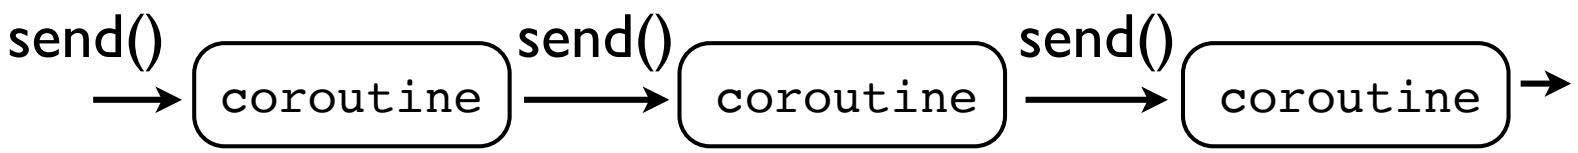
\includegraphics[keepaspectratio]{images/981f8ccb4c81fecfe797805b39e964aceb3b801cc565bd3d8a63a753291fb6ce.jpg}}

You just chain coroutines together and push data through the pipe with
send() operations

\bookmarksetup{startatroot}

\chapter{An Example}\label{an-example-1}

\bookmarksetup{startatroot}

\chapter{• A source that mimics Unix `tail
-f'}\label{a-source-that-mimics-unix-tail--f}

import time\\
def follow(filename, target): f = open(filename) f.seek(0,2) \# Go to
the end of the file while True: line \(=\) f.readline() if line \(! =\)
:: target.send(line) else: time.sleep(0.1) \# Sleep briefly=

\bookmarksetup{startatroot}

\chapter{• A consumer that just prints the
lines}\label{a-consumer-that-just-prints-the-lines}

(\textbf{consumer?})\\
def printer(): while True: line \(=\) yield print(line, end \(\equiv\)

\bookmarksetup{startatroot}

\chapter{An Example}\label{an-example-2}

\bookmarksetup{startatroot}

\chapter{A filter coroutine}\label{a-filter-coroutine}

(\textbf{consumer?})

def match(pattern, target): while True:

line \(=\) yield \# Receive a line

if pattern in line:

target.send(line) \# Send to next stage

\bookmarksetup{startatroot}

\chapter{Hooking it up}\label{hooking-it-up}

follow(`access-log', match(`python', printer()))

\bookmarksetup{startatroot}

\chapter{A picture}\label{a-picture}

\pandocbounded{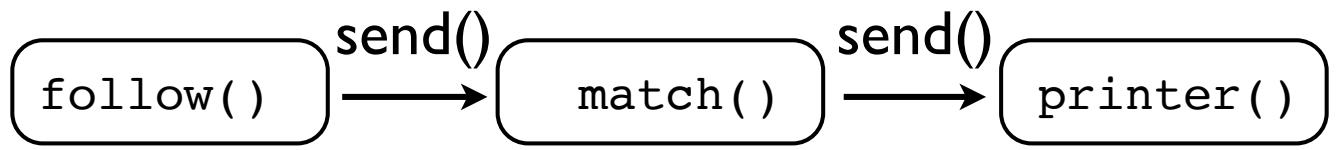
\includegraphics[keepaspectratio]{images/fcf79768b54475a25aca2f727c3bd681b7e2baa92f8f673026c89319b3810333.jpg}}

\bookmarksetup{startatroot}

\chapter{Dataflow}\label{dataflow}

• With coroutines, you can ``fan out''

\pandocbounded{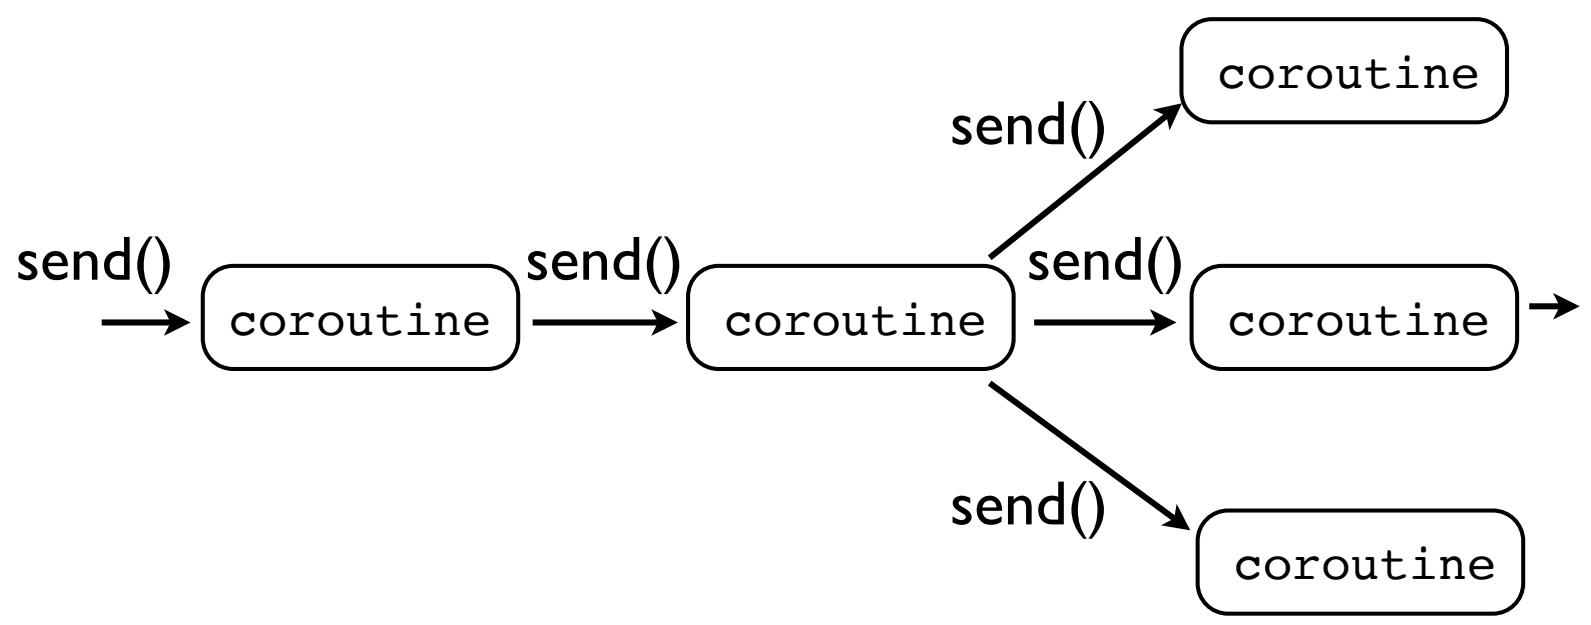
\includegraphics[keepaspectratio]{images/e0d3e36f1ee486ac5866beadd4046d7bc5d170c41cdd3384af5d3f878420647d.jpg}}

• More possibilities than a simple pipeline

\bookmarksetup{startatroot}

\chapter{Exercise 8.3}\label{exercise-8.3}

Time : 15 Minutes

\bookmarksetup{startatroot}

\chapter{Generator Control Flow}\label{generator-control-flow}

Generators have support for forced termination and exception handling

• .close() method - terminates\\
• .throw() method - raise an exception

Examples follow

\bookmarksetup{startatroot}

\chapter{Closing a Generator}\label{closing-a-generator}

• Use .close() method to shutdown

\begin{Shaded}
\begin{Highlighting}[]
\NormalTok{g = genfunc() \# A generator  }
\NormalTok{...  }
\NormalTok{g.close() }
\end{Highlighting}
\end{Shaded}

This raises GeneratorExit at yield

\begin{Shaded}
\begin{Highlighting}[]
\KeywordTok{def}\NormalTok{ genfunc():}
\NormalTok{    ...}
    \ControlFlowTok{try}\NormalTok{:}
        \ControlFlowTok{yield}\NormalTok{ item}
\ControlFlowTok{except} \PreprocessorTok{GeneratorExit}\NormalTok{:}
    \CommentTok{\# .close() was invoked}
    \CommentTok{\# perform cleanup (if any)}
\NormalTok{    ...}
    \ControlFlowTok{return} 
\end{Highlighting}
\end{Shaded}

\bookmarksetup{startatroot}

\chapter{Raising Exceptions}\label{raising-exceptions}

• Use .throw(type {[},val {[}, tb{]}{]}) for exceptions

\begin{Shaded}
\begin{Highlighting}[]
\VariableTok{g} \OperatorTok{=}\NormalTok{ genfunc}\OperatorTok{()} \OperatorTok{\#} \ConstantTok{A} \VariableTok{generator}  
\OperatorTok{...}  
\NormalTok{gthrow}\OperatorTok{(}\VariableTok{RuntimeError}\OperatorTok{,} \StringTok{"You\textquotesingle{}re dead"}\OperatorTok{)} 
\end{Highlighting}
\end{Shaded}

• This raises an exception at the yield

\begin{Shaded}
\begin{Highlighting}[]
\NormalTok{def genfunc(): try: yield item exceptRuntimeas e: \# Handle the exception }
\end{Highlighting}
\end{Shaded}

\bookmarksetup{startatroot}

\chapter{Exercise 8.4}\label{exercise-8.4}

Time : 10 Minutes

\bookmarksetup{startatroot}

\chapter{Managed Generators}\label{managed-generators}

Observation: A generator function can not execute solely by itself. It
must be driven by something else (e.g., for-loop, send(), etc)\\
Observation: The yield statement represents a point of preemption.
Generators suspend at the yield and don't resume until instructed.

\bookmarksetup{startatroot}

\chapter{Managed Generators}\label{managed-generators-1}

\bookmarksetup{startatroot}

\chapter{manager}\label{manager}

\pandocbounded{
\includegraphics[keepaspectratio]{images/694b973d37af7ad75d497247810d0417303d0632c0e7454dee2db60a47e04684.jpg}}

next() .send()

.throw() .close()

\pandocbounded{
\includegraphics[keepaspectratio]{images/4f13ae637f1c2bb4539a4bcda390565f3562158e5f5dca3fb5e39fe6f1dd0e22.jpg}}

generator

generator

generator

generator

generator

generator

Idea: A manager will coordinate the execution of a collection of
executing generators

\bookmarksetup{startatroot}

\chapter{Managed Generators}\label{managed-generators-2}

Typical applications

Concurrency (tasklets, greenlets, etc.)\\
• Actors\\
Event simulation

This is a big topic\\
• Will give a simple example

\bookmarksetup{startatroot}

\chapter{Example : Concurrency}\label{example-concurrency}

\bookmarksetup{startatroot}

\chapter{− Define some ``task''
functions}\label{define-some-task-functions}

\begin{Shaded}
\begin{Highlighting}[]
\KeywordTok{def}\NormalTok{ countdown(n):}
    \ControlFlowTok{while}\NormalTok{ n }\OperatorTok{\textgreater{}} \DecValTok{0}\NormalTok{:}
        \BuiltInTok{print}\NormalTok{(}\StringTok{\textquotesingle{}T{-}minus\textquotesingle{}}\NormalTok{, n)}
        \ControlFlowTok{yield}
\NormalTok{        n }\OperatorTok{{-}=} \DecValTok{1} 
\end{Highlighting}
\end{Shaded}

\begin{Shaded}
\begin{Highlighting}[]
\KeywordTok{def}\NormalTok{ countup(n):}
\NormalTok{    x }\OperatorTok{=} \DecValTok{0}
    \ControlFlowTok{while}\NormalTok{ x }\OperatorTok{\textless{}}\NormalTok{ n:}
        \BuiltInTok{print}\NormalTok{(}\StringTok{\textquotesingle{}Up we go\textquotesingle{}}\NormalTok{, x)}
        \ControlFlowTok{yield}
\NormalTok{        x }\OperatorTok{+=} \DecValTok{1} 
\end{Highlighting}
\end{Shaded}

\bookmarksetup{startatroot}

\chapter{• Carefully observe: just a bare
``yield''}\label{carefully-observe-just-a-bare-yield}

\bookmarksetup{startatroot}

\chapter{Example : Concurrency}\label{example-concurrency-1}

Instantiate some tasks in a queue

\begin{Shaded}
\begin{Highlighting}[]
\NormalTok{tasks = deque([countdown(10), countdown(5), countup(20)] }
\end{Highlighting}
\end{Shaded}

Run a little scheduler (the manager)

\begin{Shaded}
\begin{Highlighting}[]
\KeywordTok{def}\NormalTok{ run():}
    \ControlFlowTok{while}\NormalTok{ tasks:}
\NormalTok{        t }\OperatorTok{=}\NormalTok{ tasks.popleft()}
        \ControlFlowTok{try}\NormalTok{:}
\NormalTok{            t.send(}\VariableTok{None}\NormalTok{)}
\NormalTok{            tasks.append(t)  }\CommentTok{\# Run to yield}
            \ControlFlowTok{except} \PreprocessorTok{StopIteration}\NormalTok{:}
                \ControlFlowTok{pass} 
\end{Highlighting}
\end{Shaded}

\bookmarksetup{startatroot}

\chapter{Example : Concurrency}\label{example-concurrency-2}

\bookmarksetup{startatroot}

\chapter{Output}\label{output}

\begin{Shaded}
\begin{Highlighting}[]
\NormalTok{T{-}minus 10  }
\NormalTok{T{-}minus 5  }
\NormalTok{Up we go 0  }
\NormalTok{T{-}minus 9  }
\NormalTok{T{-}minus 4  }
\NormalTok{Up we go 1  }
\NormalTok{T{-}minus 8  }
\NormalTok{T{-}minus 4  }
\NormalTok{Up we go 2  }
\NormalTok{... }
\end{Highlighting}
\end{Shaded}

• We see tasks cycling, but there are no threads

\bookmarksetup{startatroot}

\chapter{Exercise 8.5}\label{exercise-8.5}

Time : 20 Minutes

\bookmarksetup{startatroot}

\chapter{Delegating Generation}\label{delegating-generation}

• Problem: Library functions involving generators

\begin{Shaded}
\begin{Highlighting}[]
\KeywordTok{def}\NormalTok{ countdown(n):}
    \ControlFlowTok{while}\NormalTok{ n }\OperatorTok{\textgreater{}} \DecValTok{0}\NormalTok{:}
        \ControlFlowTok{yield}\NormalTok{ n}
\NormalTok{        n }\OperatorTok{{-}=} \DecValTok{1} 
\end{Highlighting}
\end{Shaded}

\begin{Shaded}
\begin{Highlighting}[]
\KeywordTok{def}\NormalTok{ countup(end): n }\OperatorTok{=} \DecValTok{0} \ControlFlowTok{while}\NormalTok{ n }\OperatorTok{\textless{}}\NormalTok{ end: }\ControlFlowTok{yield}\NormalTok{ n n }\OperatorTok{+=} \DecValTok{1} 
\end{Highlighting}
\end{Shaded}

\begin{Shaded}
\begin{Highlighting}[]
\KeywordTok{def}\NormalTok{ up\_and\_down(n):}
\NormalTok{    countup(n)}
\NormalTok{    countdown(n) }
\end{Highlighting}
\end{Shaded}

Problem: It doesn't run\ldots{}\\
• Generators can't run on their own.

\bookmarksetup{startatroot}

\chapter{Delegating Generation}\label{delegating-generation-1}

• Option 1: Drive the generator yourself

\begin{Shaded}
\begin{Highlighting}[]
\KeywordTok{def}\NormalTok{ up\_and\_down(n):}
    \ControlFlowTok{for}\NormalTok{ x }\KeywordTok{in}\NormalTok{ countup(n):}
        \ControlFlowTok{yield}\NormalTok{ x}
    \ControlFlowTok{for}\NormalTok{ x }\KeywordTok{in}\NormalTok{ countdown(n):}
        \ControlFlowTok{yield}\NormalTok{ x }
\end{Highlighting}
\end{Shaded}

You need to manually control each generator with for-loops, send(),
throw(), etc.\\
• Can get quite complicated for coroutines

\bookmarksetup{startatroot}

\chapter{Delegating Generation}\label{delegating-generation-2}

• Option 2: Let Python drive it (yield from)

def up\_and\_down(n): yield from countup(n) yield from countdown(n)

Whatever ``outer'' code runs the generator will take care of it (you
don't worry about it)

for x in up\_and\_down(5): \# 0,1,2,3,4,5,4,3,2,1 \ldots{}

\bookmarksetup{startatroot}

\chapter{Async/Await}\label{asyncawait}

• Alternate syntax for defining a coroutine (async)

async def greeting(name): return f'Hello \{name\}'

\begin{Shaded}
\begin{Highlighting}[]
\NormalTok{\textgreater{}\textgreater{}\textgreater{} g = greeting(\textquotesingle{}Guido\textquotesingle{})}
\NormalTok{\textgreater{}\textgreater{}\textgreater{} g}
\NormalTok{\textless{}coroutine object greeting at 0x10b8b8258\textgreater{}}
\NormalTok{\textgreater{}\textgreater{}\textgreater{} g.send(None)}
\NormalTok{Traceback (most recent call last):}
\NormalTok{    File "\textless{}stdin\textgreater{}", line 1, in \textless{}module\textgreater{}}
\NormalTok{StopIteration: Hello Guido }
\end{Highlighting}
\end{Shaded}

Syntax for calling a coroutine (await)

\begin{Shaded}
\begin{Highlighting}[]
\ControlFlowTok{async} \KeywordTok{def}\NormalTok{ main(): names }\OperatorTok{=}\NormalTok{ [}\StringTok{\textquotesingle{}Guido\textquotesingle{}}\NormalTok{, }\StringTok{\textquotesingle{}Dave\textquotesingle{}}\NormalTok{, }\StringTok{\textquotesingle{}Paula\textquotesingle{}}\NormalTok{] }\ControlFlowTok{for}\NormalTok{ name }\KeywordTok{in}\NormalTok{ names: g }\OperatorTok{=} \ControlFlowTok{await}\NormalTok{ greeting(name) }\BuiltInTok{print}\NormalTok{(g) }
\end{Highlighting}
\end{Shaded}

\bookmarksetup{startatroot}

\chapter{Async/Await}\label{asyncawait-1}

async/await mainly associated with asynchronous I/O, the asyncio module,
and related tools\\
• Provides a better environment for multitasking\\
• The topic of a whole different course\\
See: ``Fear and Awaiting in Async''

https://www.youtube.com/watch?v=E-1Y4kSsAFc

\bookmarksetup{startatroot}

\chapter{More Information}\label{more-information}

``Generator Tricks for Systems Programmers'' tutorial from PyCon'08
http://www.dabeaz.com/generators\\
• ``A Curious Course on Coroutines and Concurrency'' tutorial from
PyCon'09 http://www.dabeaz.com/coroutines\\
``Generators: The Final Frontier'' tutorial from PyCon'14
http://www.dabeaz.com/finalgenerator

\bookmarksetup{startatroot}

\chapter{Exercise 8.6}\label{exercise-8.6}

Time : 15 Minutes

\bookmarksetup{startatroot}

\chapter{Section 9}\label{section-9}

\bookmarksetup{startatroot}

\chapter{Modules and Packages}\label{modules-and-packages}

\bookmarksetup{startatroot}

\chapter{Introduction}\label{introduction-1}

You've written some code\\
• Now you need to organize it\\
• Possibly give it to others\\
• How do you do it?

\bookmarksetup{startatroot}

\chapter{Modules Revisited}\label{modules-revisited}

• As you know, every source file is a module

\begin{Shaded}
\begin{Highlighting}[]
\NormalTok{foo.py def grok(a): def spam(b): }
\end{Highlighting}
\end{Shaded}

• import statement loads and executes a module

\begin{Shaded}
\begin{Highlighting}[]
\NormalTok{import foo  }
\NormalTok{a = foo.grok(2)  }
\NormalTok{b = foo.spam(\textquotesingle{}Hello\textquotesingle{})  }
\NormalTok{... }
\end{Highlighting}
\end{Shaded}

\bookmarksetup{startatroot}

\chapter{Module Objects}\label{module-objects}

Modules are objects

\begin{Shaded}
\begin{Highlighting}[]
\NormalTok{\textgreater{}\textgreater{}\textgreater{} import foo}
\NormalTok{\textgreater{}\textgreater{}\textgreater{} foo}
\NormalTok{\textless{}module \textquotesingle{}foo\textquotesingle{} from \textquotesingle{}foo.py\textgreater{}}
\NormalTok{\textgreater{}\textgreater{}\textgreater{} }
\end{Highlighting}
\end{Shaded}

• A ``namespace'' for definitions inside

\begin{Shaded}
\begin{Highlighting}[]
\NormalTok{\textgreater{}\textgreater{}\textgreater{} foo.grok(2)  }
\NormalTok{\textgreater{}\textgreater{}\textgreater{} }
\end{Highlighting}
\end{Shaded}

• Actually a layer on top of a dictionary (globals)

\begin{Shaded}
\begin{Highlighting}[]
\NormalTok{\textgreater{}\textgreater{}\textgreater{} foo.\_\_dict\_\_[\textquotesingle{}grok\textquotesingle{}]}
\DataTypeTok{\textless{}}\KeywordTok{function}\OtherTok{ grok at }\ErrorTok{0x1006b6c80}\DataTypeTok{\textgreater{}}
\NormalTok{\textgreater{}\textgreater{}\textgreater{} }
\end{Highlighting}
\end{Shaded}

\bookmarksetup{startatroot}

\chapter{Special Variables}\label{special-variables}

• A few special variables defined in a module

\begin{Shaded}
\begin{Highlighting}[]
\VariableTok{\_\_file\_\_} \CommentTok{\# Name of the source file  }
\VariableTok{\_\_name\_\_} \CommentTok{\# Name of the module  }
\NormalTok{\_\_doc\_\_ }\CommentTok{\# Module documentation string }
\end{Highlighting}
\end{Shaded}

Example: ``main'' check

\begin{Shaded}
\begin{Highlighting}[]
\ControlFlowTok{if} \VariableTok{\_\_name\_\_} \OperatorTok{==} \StringTok{\textquotesingle{}\_\_main\_\_\textquotesingle{}}\NormalTok{:}
    \BuiltInTok{print}\NormalTok{(}\StringTok{\textquotesingle{}Running as the main program\textquotesingle{}}\NormalTok{)}
\ControlFlowTok{else}\NormalTok{:}
    \BuiltInTok{print}\NormalTok{(}\StringTok{\textquotesingle{}Imported as a module using import\textquotesingle{}}\NormalTok{) }
\end{Highlighting}
\end{Shaded}

\bookmarksetup{startatroot}

\chapter{Import Implementation}\label{import-implementation}

\bookmarksetup{startatroot}

\chapter{Import in a nutshell
(pseudocode)}\label{import-in-a-nutshell-pseudocode}

import types

\begin{Shaded}
\begin{Highlighting}[]
\KeywordTok{def}\NormalTok{ import\_module(name):}
    \CommentTok{\# locate the module and get source code}
\NormalTok{    filename }\OperatorTok{=}\NormalTok{ find\_module(name)}
\NormalTok{    code }\OperatorTok{=} \BuiltInTok{open}\NormalTok{(filename).read() }
\end{Highlighting}
\end{Shaded}

\begin{Shaded}
\begin{Highlighting}[]
\NormalTok{Create the enclosing module object mod = types\_Module(name) }
\end{Highlighting}
\end{Shaded}

\begin{Shaded}
\begin{Highlighting}[]
\NormalTok{Run it exec(code, mod.\_\_dict\_\_, mod.\_\_dict\_\_) return mod }
\end{Highlighting}
\end{Shaded}

Source is exec'd in module dictionary\\
• Contents are whatever is left over

\bookmarksetup{startatroot}

\chapter{import statement}\label{import-statement}

import executes the entire module

\begin{Shaded}
\begin{Highlighting}[]
\NormalTok{bar.py import foo}
\end{Highlighting}
\end{Shaded}

It inserts a name reference to the module object into the dictionary
used by the code that made the import

\pandocbounded{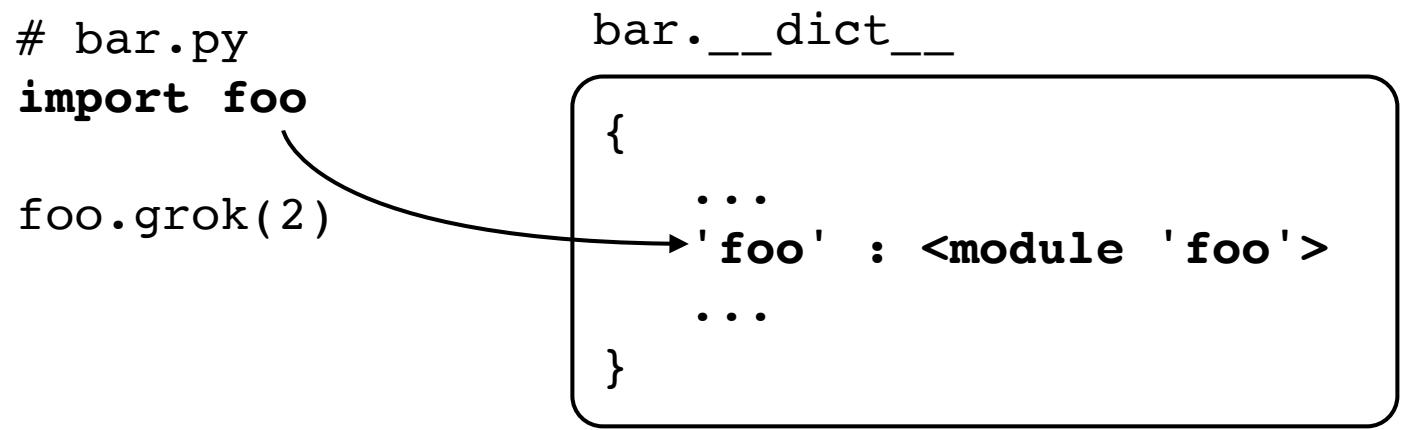
\includegraphics[keepaspectratio]{images/62bd43ed7ddee3db9f1fb9581992e9f7d319232b04895021c2caf5879bc7dac5.jpg}}

\bookmarksetup{startatroot}

\chapter{Module Cache}\label{module-cache}

Each module is loaded only once\\
Repeated imports just return a reference to the previously loaded
module\\
sys.modules is a dict of all loaded modules

\begin{Shaded}
\begin{Highlighting}[]
\OperatorTok{\textgreater{}\textgreater{}\textgreater{}} \ImportTok{import}\NormalTok{ sys   }
\OperatorTok{\textgreater{}\textgreater{}\textgreater{}} \BuiltInTok{list}\NormalTok{(sys}\OperatorTok{/}\NormalTok{modules)   }
\NormalTok{[}\StringTok{\textquotesingle{}copy\_reg\textquotesingle{}}\NormalTok{, }\StringTok{\textquotesingle{}\_\_main\_\_\textquotesingle{}}\NormalTok{, }\StringTok{\textquotesingle{}site\textquotesingle{}}\NormalTok{, }\StringTok{\textquotesingle{}\_\_builtin\_\_\textquotesingle{}}\NormalTok{,   }
\StringTok{\textquotesingle{}encodings\textquotesingle{}}\NormalTok{, }\StringTok{\textquotesingle{}encodings.ENCODINGS\textquotesingle{}}\NormalTok{, }\StringTok{\textquotesingle{}posixpath\textquotesingle{}}\NormalTok{, ...]   }
\OperatorTok{\textgreater{}\textgreater{}\textgreater{}} 
\end{Highlighting}
\end{Shaded}

\bookmarksetup{startatroot}

\chapter{Import Caching}\label{import-caching}

\bookmarksetup{startatroot}

\chapter{Import (pseudocode)}\label{import-pseudocode}

import types import sys

\begin{Shaded}
\begin{Highlighting}[]
\KeywordTok{def}\NormalTok{ import\_module(name):}
    \CommentTok{\# Check for cached module}
    \ControlFlowTok{if}\NormalTok{ name }\KeywordTok{in}\NormalTok{ sys}\OperatorTok{/}\NormalTok{modules:}
        \ControlFlowTok{return}\NormalTok{ sys}\OperatorTok{/}\NormalTok{modules[name]}
\NormalTok{    filename }\OperatorTok{=}\NormalTok{ find\_module(name)}
\NormalTok{    code }\OperatorTok{=} \BuiltInTok{open}\NormalTok{(filename).read()}
\NormalTok{    mod }\OperatorTok{=}\NormalTok{ typesModuleType(name)}
\NormalTok{    sys}\OperatorTok{/}\NormalTok{modules[name] }\OperatorTok{=}\NormalTok{ mod }
\end{Highlighting}
\end{Shaded}

\begin{Shaded}
\begin{Highlighting}[]
\BuiltInTok{exec}\NormalTok{(code, mod.\_\_dict\_\_, mod.\_\_dict\_\_) }\ControlFlowTok{return}\NormalTok{ mod }
\end{Highlighting}
\end{Shaded}

\bookmarksetup{startatroot}

\chapter{• There is more, but this is basically
it}\label{there-is-more-but-this-is-basically-it}

\bookmarksetup{startatroot}

\chapter{from module import}\label{from-module-import-3}

• Selected symbols can be imported locally

\bookmarksetup{startatroot}

\chapter{bar.py}\label{bar.py}

from foo import grok

grok(2)

• Useful for frequently used names\\
Confusion: This does not change how import works. The entire module
executes and is cached. This merely copies a name.

\[
\text {g r o k} = \text {s y s . m o d u l e s} [ ^ {\prime} f o o ^ {\prime} ] \cdot \text {g r o k}
\]

\bookmarksetup{startatroot}

\chapter{from module import *}\label{from-module-import-4}

Takes all symbols from a module and places them into the caller's
namespace

\bookmarksetup{startatroot}

\chapter{bar.py from foo import *}\label{bar.py-from-foo-import}

grok(2) spam(`Hello')

However, it only applies to names that don't start with an underscore
(\_)\\
\_name often used when defining nonimported values in a module.

\bookmarksetup{startatroot}

\chapter{Module Reloading}\label{module-reloading}

• Modules can sometimes be reloaded

\begin{Shaded}
\begin{Highlighting}[]
\OperatorTok{\textgreater{}\textgreater{}\textgreater{}} \KeywordTok{import}\NormalTok{ foo   }
\OperatorTok{\textgreater{}\textgreater{}\textgreater{}} \KeywordTok{import}\NormalTok{ importlib   }
\OperatorTok{\textgreater{}\textgreater{}\textgreater{}}\NormalTok{ importlib}\OperatorTok{.}\NormalTok{reload(foo)   }
\OperatorTok{\textless{}}\KeywordTok{module}\NormalTok{ \textquotesingle{}foo\textquotesingle{} from \textquotesingle{}foo}\OperatorTok{.}\NormalTok{py\textquotesingle{}}\OperatorTok{\textgreater{}}   
\OperatorTok{\textgreater{}\textgreater{}\textgreater{}} 
\end{Highlighting}
\end{Shaded}

It re-executes the module source on top of the already defined module
dictionary

\begin{Shaded}
\begin{Highlighting}[]
\CommentTok{\# pseudocode}
\KeywordTok{def} \BuiltInTok{reload}\NormalTok{(mod):}
\NormalTok{    code }\OperatorTok{=} \BuiltInTok{open}\NormalTok{(mod.}\VariableTok{\_\_file\_\_}\NormalTok{, }\StringTok{\textquotesingle{}r\textquotesingle{}}\NormalTok{).read()}
    \BuiltInTok{exec}\NormalTok{(code, mod.\_\_dict\_\_, mod.\_\_dict\_\_).}
\ControlFlowTok{return}\NormalTok{ mod }
\end{Highlighting}
\end{Shaded}

\bookmarksetup{startatroot}

\chapter{Module Reloading Danger}\label{module-reloading-danger}

Module reloading is not advised\\
Problem: Existing instances of classes will continue to use old code
after reload\\
Problem: Doesn't update definitions loaded with `from module import
name'\\
Problem: Likely breaks code that performs typechecks or uses super()

\bookmarksetup{startatroot}

\chapter{Locating Modules}\label{locating-modules-1}

When looking for modules, Python first looks in the same directory as
the source file that's executing the import\\
If a module can't be found there, an internal module search path is
consulted

\begin{Shaded}
\begin{Highlighting}[]
\NormalTok{\textgreater{}\textgreater{}\textgreater{} import sys   }
\NormalTok{\textgreater{}\textgreater{}\textgreater{} sys.path   }
\NormalTok{[\textquotesingle{}\textquotesingle{}, \textquotesingle{}/usr/local/lib/python36.zip\textquotesingle{}， \textquotesingle{}/usr/local/lib/python3.6\textquotesingle{}， \textquotesingle{}/usr/local/lib/python3.6/plat{-}darwin\textquotesingle{}， \textquotesingle{}/usr/local/lib/python3.6/lib{-}dynload\textquotesingle{}，\textquotesingle{}/usr/local/lib/python3.6/site{-}packages\textquotesingle{}]}
\end{Highlighting}
\end{Shaded}

\bookmarksetup{startatroot}

\chapter{Module Search Path}\label{module-search-path-1}

sys.path contains search path\\
• Can manually adjust if you need to

import sys

sys.path.append(`/project/foo/pyfiles')

Paths also added via environment variables

\begin{Shaded}
\begin{Highlighting}[]
\NormalTok{\% env PATH=/project/foo/pyfiles python3   }
\NormalTok{Python 3.6.0 (default, Jan 12 2017, 13:20:23)   }
\NormalTok{[GCC 4.2.1 Compatible Apple LLVM 6.1.0 (clang{-}602.0.53)]   }
\NormalTok{\textgreater{}\textgreater{}\textgreater{} import sys   }
\NormalTok{\textgreater{}\textgreater{}\textgreater{} sys.path   }
\NormalTok{[\textquotesingle{}\textquotesingle{}, \textquotesingle{}/project/foo/pyfiles\textquotesingle{}, \textquotesingle{}/usr/local/lib/python36.zip\textquotesingle{}, ... ] }
\end{Highlighting}
\end{Shaded}

\bookmarksetup{startatroot}

\chapter{Exercise 9.}\label{exercise-9.}

10 minutes

\bookmarksetup{startatroot}

\chapter{Organizing Libraries}\label{organizing-libraries}

It is standard practice for Python libraries to be organized as a
hierarchical set of modules that sit under a top-level package name

\begin{Shaded}
\begin{Highlighting}[]
\NormalTok{packagename  }
\NormalTok{packagename.foo  }
\NormalTok{packagename.bar  }
\NormalTok{packagename.utils  }
\NormalTok{packagename.utils.spam  }
\NormalTok{packagename.utils.grok  }
\NormalTok{packagename.parsers  }
\NormalTok{packagename.parsers.xml  }
\NormalTok{packagename.parsers.json  }
\NormalTok{... }
\end{Highlighting}
\end{Shaded}

Other programming languages have a similar convention (e.g., Java)

\bookmarksetup{startatroot}

\chapter{Creating a Package}\label{creating-a-package}

• To create the module library hierarchy, organize files on the
filesystem in a directory with the desired structure

\begin{Shaded}
\begin{Highlighting}[]
\NormalTok{packagename/ foo.py bar.py utils/ spam.py grok.py parsers/ xml.py json.py }
\end{Highlighting}
\end{Shaded}

\bookmarksetup{startatroot}

\chapter{Creating a Package}\label{creating-a-package-1}

• Add \textbf{init}.py files to each directory

\begin{Shaded}
\begin{Highlighting}[]
\NormalTok{package name/  }
\NormalTok{\_\_init\_\_.py  }
\NormalTok{foo.py  }
\NormalTok{bar.py  }
\NormalTok{utils/  }
\NormalTok{\_\_init\_\_.py  }
\NormalTok{spam.py  }
\NormalTok{grok.py  }
\NormalTok{ parsers/  }
\NormalTok{\_\_init\_\_.py  }
\NormalTok{xml.py  }
\NormalTok{json.py}
\end{Highlighting}
\end{Shaded}

• These can be empty, but they should exist

\bookmarksetup{startatroot}

\chapter{Using a Package}\label{using-a-package}

Once you have the \textbf{init}.py files, the import statement should
just ``work''

import packagename.foo

import packagename.parsers.xml

from packagename.parsers import xml

Almost everything should work the same way that it did before except
that import statements now have multiple levels

\bookmarksetup{startatroot}

\chapter{Fixing Relative Imports}\label{fixing-relative-imports}

Relative imports of submodules don't work

spam/

init\_\_.pyfoo.pybar.py

\bookmarksetup{startatroot}

\chapter{bar.py import foo \# Fails (not
found)}\label{bar.py-import-foo-fails-not-found}

The issue: Resolving name clashes between top-level packages and
submodules

spam/

init\_\_.pyos.pybar.py

\bookmarksetup{startatroot}

\chapter{bar.py import os \# ??? (uses
stdlib)}\label{bar.py-import-os-uses-stdlib}

imports are always ``absolute'' (from top level)

\bookmarksetup{startatroot}

\chapter{Absolute Imports}\label{absolute-imports}

• One approach : use absolute imports

\begin{Shaded}
\begin{Highlighting}[]
\NormalTok{spam/ init.py foo.py bar.py }
\end{Highlighting}
\end{Shaded}

• Example :

\begin{Shaded}
\begin{Highlighting}[]
\NormalTok{bar.py from spam import foo }
\end{Highlighting}
\end{Shaded}

• Notice use of top-level package name

\bookmarksetup{startatroot}

\chapter{Package Relative Imports}\label{package-relative-imports}

Consider a package

\begin{Shaded}
\begin{Highlighting}[]
\NormalTok{spam/ \_\_init\_\_.py foo.py bar.py grok/ \_\_init\_\_.py blah.py }
\end{Highlighting}
\end{Shaded}

Package relative imports

\bookmarksetup{startatroot}

\chapter{bar.py}\label{bar.py-1}

\begin{Shaded}
\begin{Highlighting}[]
\ImportTok{from}\NormalTok{ . }\ImportTok{import}\NormalTok{ foo }\CommentTok{\# Imports ./foo.py  }
\ImportTok{from}\NormalTok{ . foo }\ImportTok{import}\NormalTok{ name }\CommentTok{\# Load a specific name  }
\ImportTok{from}\NormalTok{ . grok }\ImportTok{import}\NormalTok{ blah }\CommentTok{\# Imports ./grok/blah.py }
\end{Highlighting}
\end{Shaded}

\bookmarksetup{startatroot}

\chapter{Package Environment}\label{package-environment}

Packages define a few useful variables

\begin{Shaded}
\begin{Highlighting}[]
\NormalTok{\_\_package\_\_ \_\_path\_\_ }
\end{Highlighting}
\end{Shaded}

\begin{Shaded}
\begin{Highlighting}[]
\NormalTok{Name of the enclosing package \# Search path for subcomponents }
\end{Highlighting}
\end{Shaded}

Example:

\begin{Shaded}
\begin{Highlighting}[]
\NormalTok{\textgreater{}\textgreater{}\textgreater{} import xml}
\NormalTok{\textgreater{}\textgreater{}\textgreater{} xml.\_package\_\_}
\NormalTok{\textquotesingle{}xml\textquotesingle{}}
\NormalTok{\textgreater{}\textgreater{}\textgreater{} xml.\_path\_\_}
\NormalTok{[\textquotesingle{}/usr/local/lib/python3.5/xml\textquotesingle{}] }
\end{Highlighting}
\end{Shaded}

• Useful if code needs to obtain information about its enclosing
environment

\bookmarksetup{startatroot}

\chapter{Exercise 9.2}\label{exercise-9.2}

10 minutes

\bookmarksetup{startatroot}

\chapter{init \_.py Usage}\label{init-_.py-usage}

• What are you supposed to do in those files?\\
Main use: stitching together multiple source files into a ``unified''
top-level import

\bookmarksetup{startatroot}

\chapter{Module Assembly}\label{module-assembly}

• Consider two submodules in a package

spam/

foo.py

\bookmarksetup{startatroot}

\chapter{foo.py}\label{foo.py}

class Foo:

bar.py

\pandocbounded{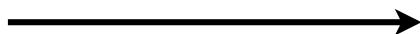
\includegraphics[keepaspectratio]{images/5f042d3aa59f4ad6d93850f24758de21baebd20de08861b0aa9b23be2b5fb3f9.jpg}}

\bookmarksetup{startatroot}

\chapter{bar.py}\label{bar.py-2}

class Bar:

• Suppose you wanted to combine them

\bookmarksetup{startatroot}

\chapter{Module Assembly}\label{module-assembly-1}

Combine in \_init\_\_.py

\pandocbounded{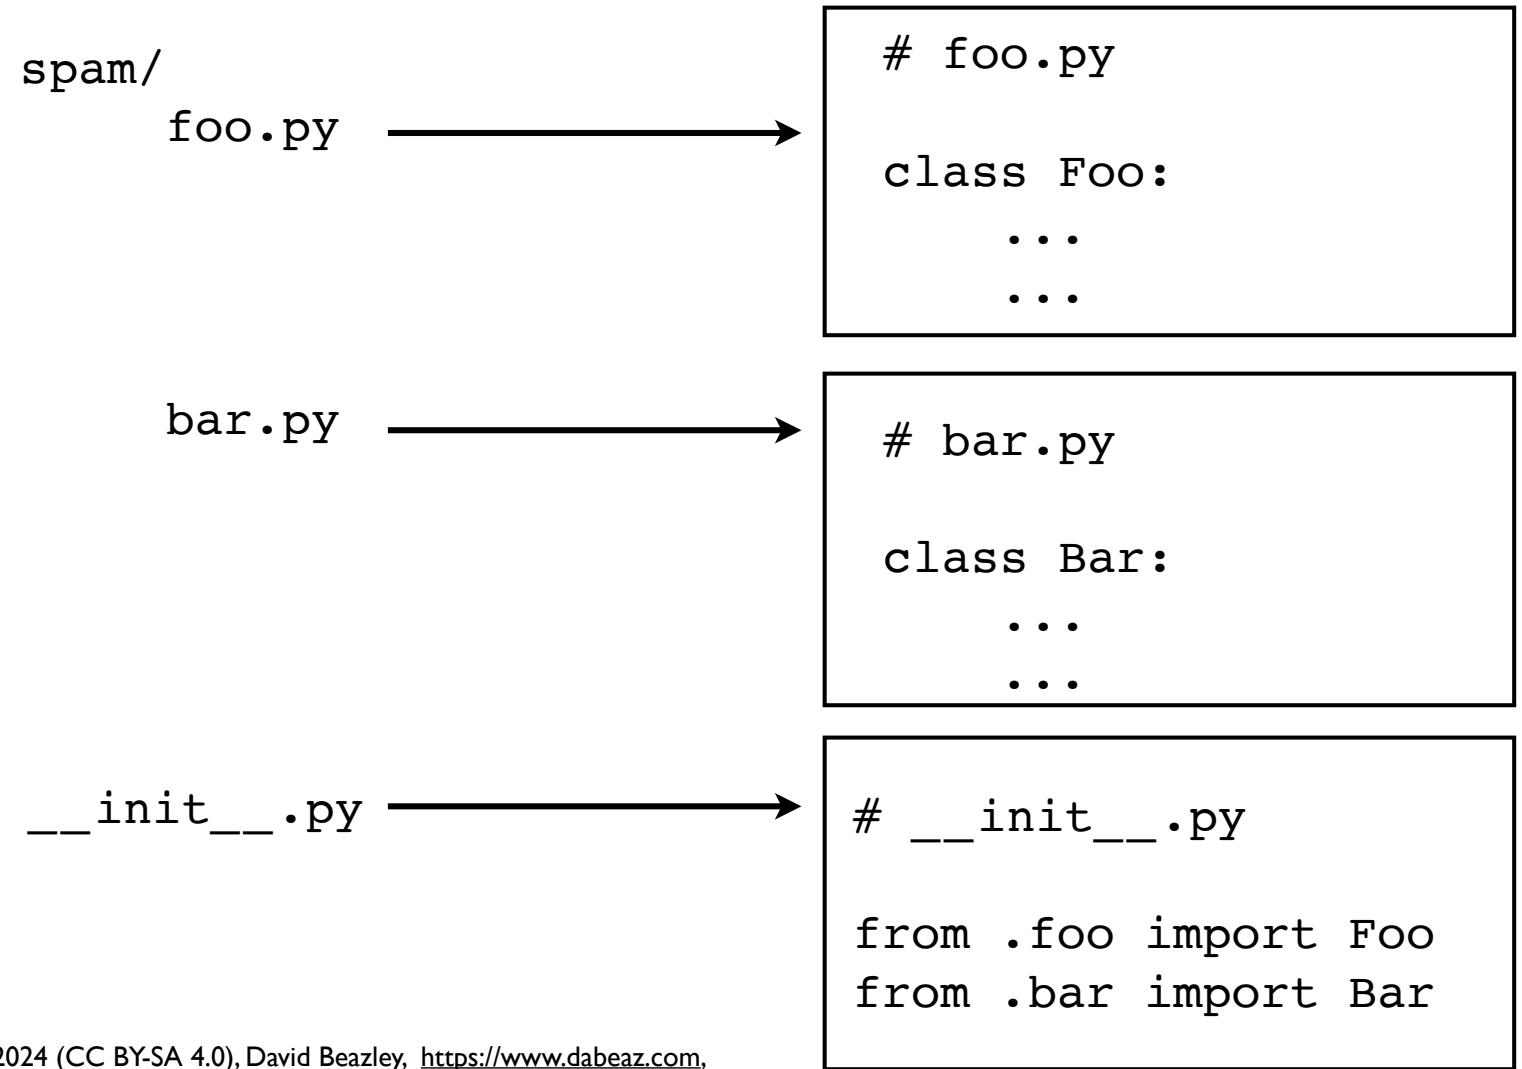
\includegraphics[keepaspectratio]{images/b6f1314113e2cced2096da8f139dccec02f69cf4e4b70a65322398526355f5cb.jpg}}

\bookmarksetup{startatroot}

\chapter{Module Assembly}\label{module-assembly-2}

• Users see a single unified top-level package

import spam

\[
f = \operatorname {s p a m}. F o o (  )
\]

\[
b = \text {s p a m . B a r ()}
\]

\[
\begin{array}{c c c} \bullet & \bullet & \bullet \\ \hline \end{array}
\]

Split across submodules is hidden

\bookmarksetup{startatroot}

\chapter{Case Study}\label{case-study}

The collections ``module''\\
• It's actually a package with a few components

\pandocbounded{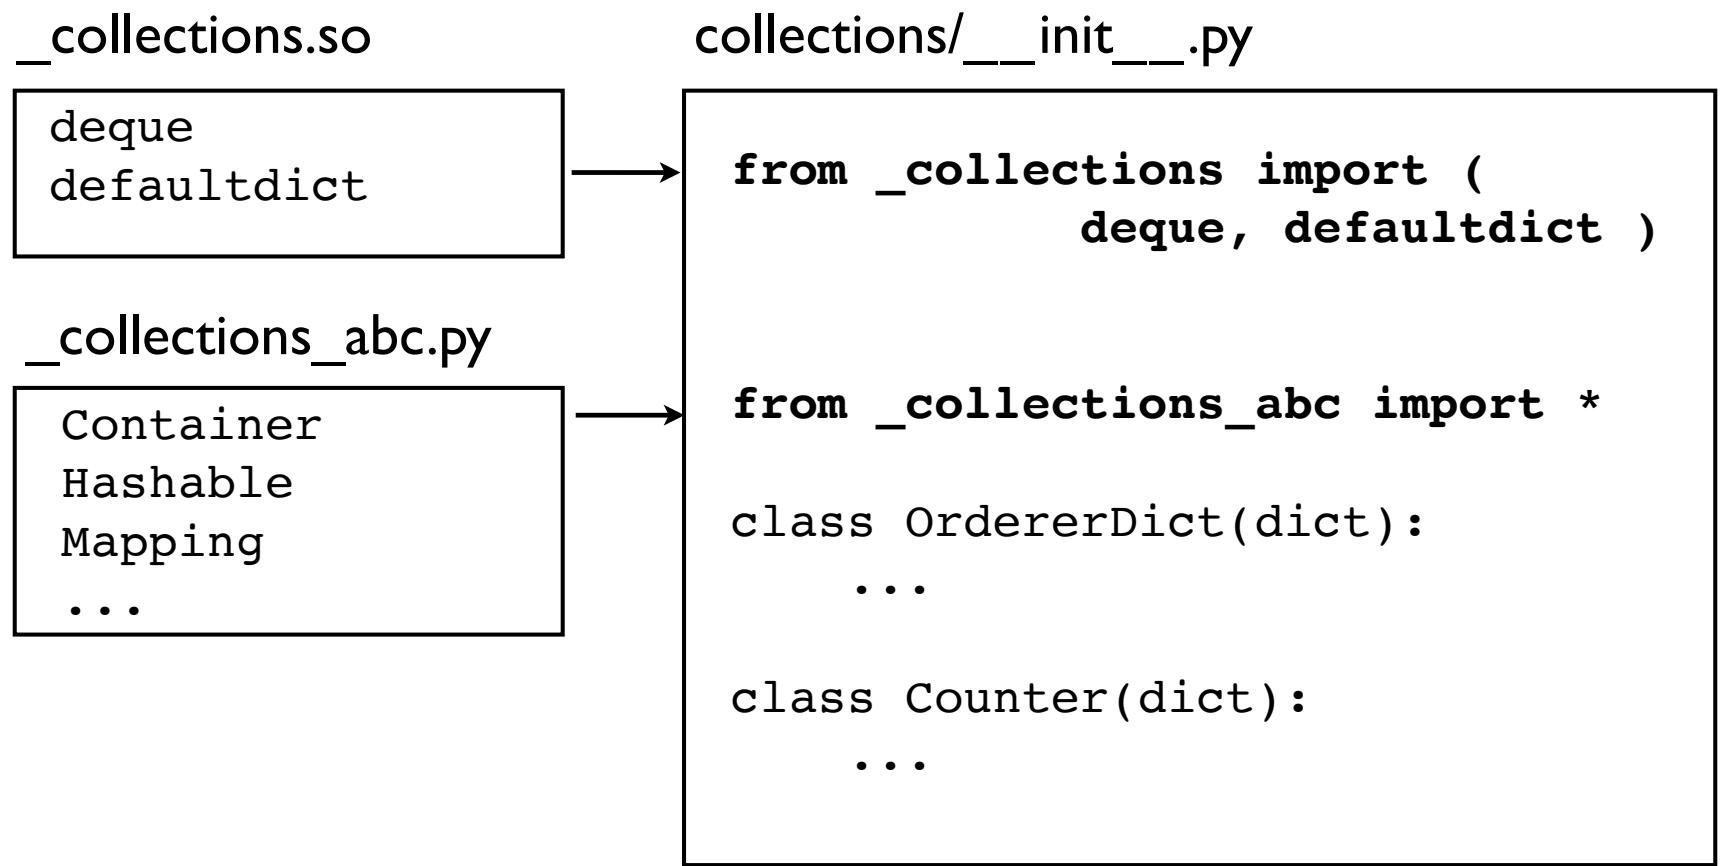
\includegraphics[keepaspectratio]{images/30695d7f4538151dbb5b37341bfb70cdb2000bd3ffc6f3ffe79392269ed5f586.jpg}}

\bookmarksetup{startatroot}

\chapter{Controlling Exports}\label{controlling-exports}

Submodules should define \_\_all\_

\bookmarksetup{startatroot}

\chapter{foo.py}\label{foo.py-1}

\bookmarksetup{startatroot}

\chapter{bar.py}\label{bar.py-3}

\textbf{all} = {[}`Foo'{]}

\textbf{all} = {[}`Bar'{]}

class Foo(object):

class Bar(object):

Controls 'from module import *'\\
• Allows easy combination in \textbf{init}.py

\bookmarksetup{startatroot}

\chapter{\texorpdfstring{\textbf{init}.py}{init.py}}\label{init.py}

from .foo import *

from .bar import *

\textbf{all} = {[} *foo.\_\_all\_\_, *bar.\_\_all\_\_ {]}

\bookmarksetup{startatroot}

\chapter{Module Splitting}\label{module-splitting}

• Suppose you have a large module

\bookmarksetup{startatroot}

\chapter{spam.py}\label{spam.py}

class Foo:

class Bar:

• You want to split it into multiple files\\
But keep it as a single import

\bookmarksetup{startatroot}

\chapter{Module Splitting}\label{module-splitting-1}

• Step 1: Turn into a directory with multiple files

\pandocbounded{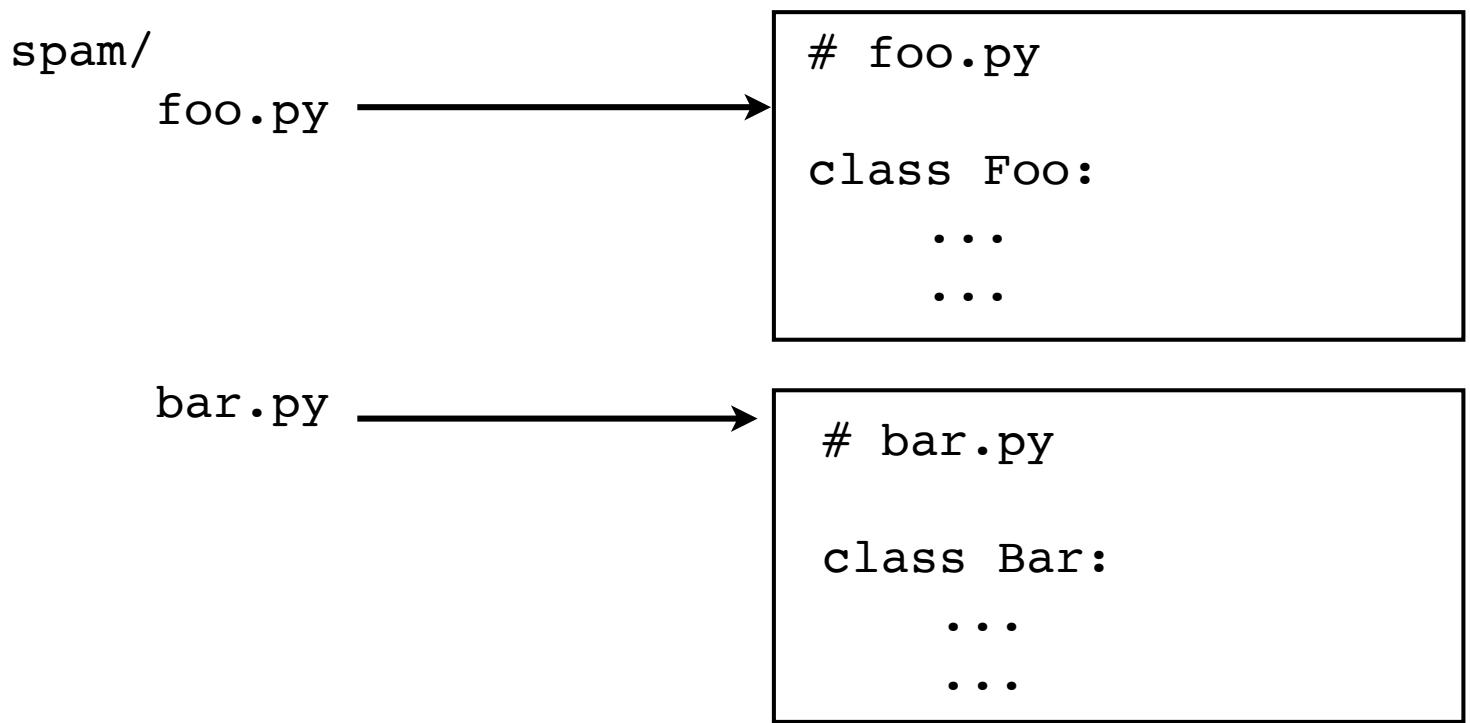
\includegraphics[keepaspectratio]{images/911e94e28c1d8cc4f62190cf354332102cce4c2ec2c83b36e070c00c35983b89.jpg}}

Split the code you wish

\bookmarksetup{startatroot}

\chapter{Module Splitting}\label{module-splitting-2}

• Step 2: Stitch back together in \textbf{init}.py

\pandocbounded{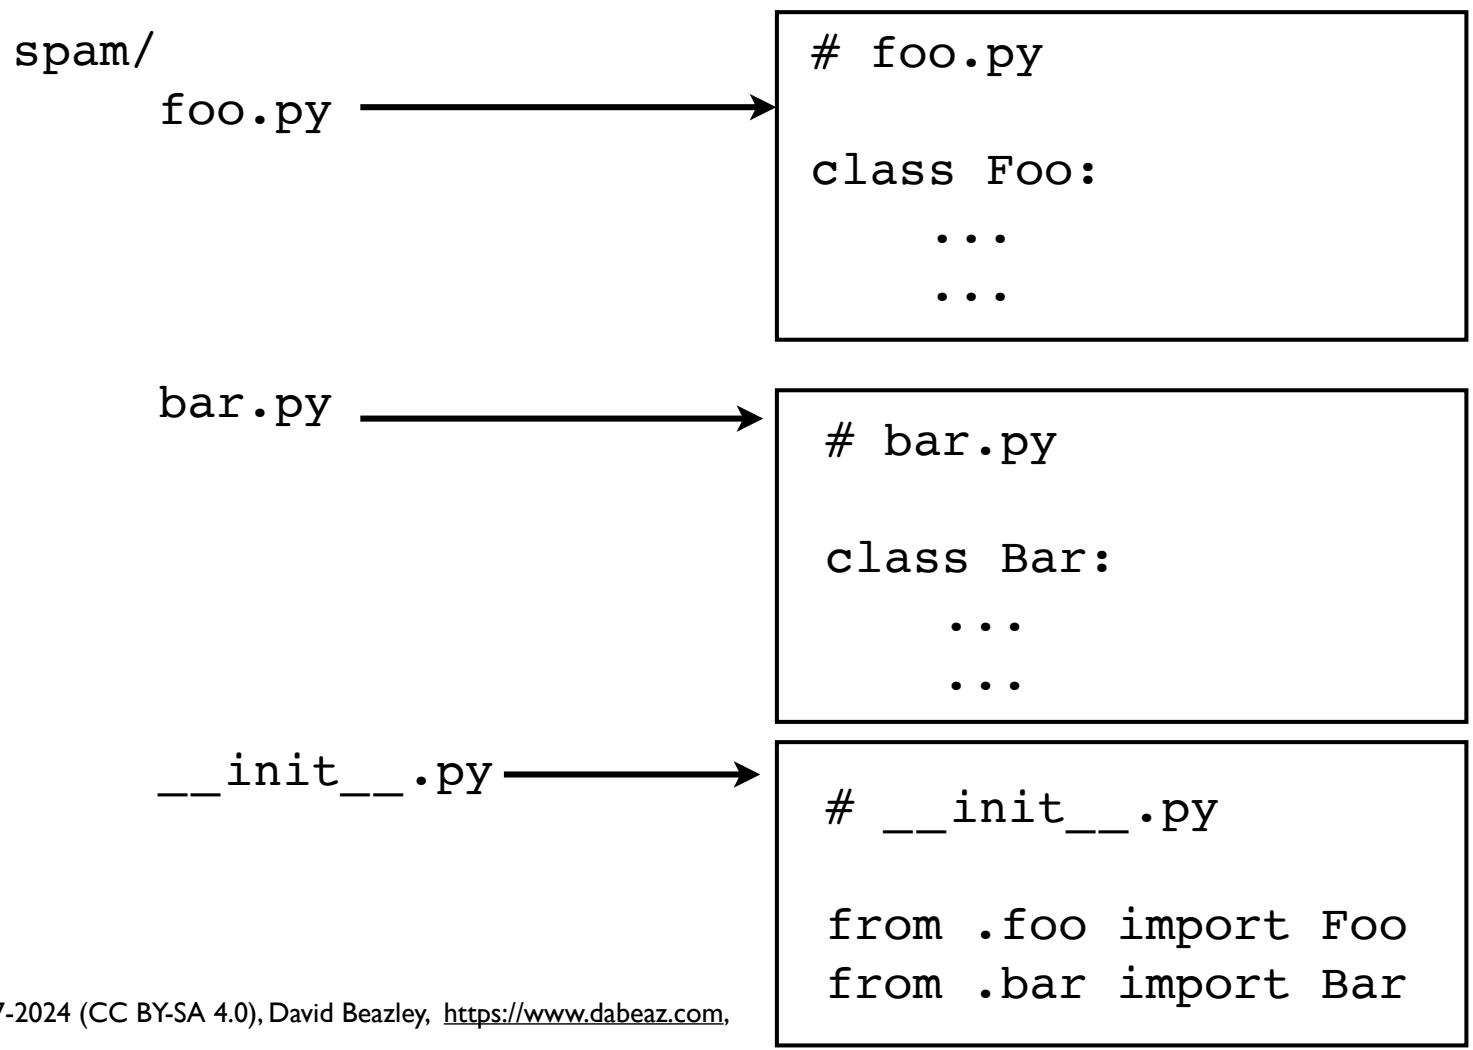
\includegraphics[keepaspectratio]{images/0d1c35061661a98420cd9f5f60780592b1128d5d4d053871a624f6234253d6ad.jpg}}

\bookmarksetup{startatroot}

\chapter{Exercise 9.3}\label{exercise-9.3}

20 minutes

\bookmarksetup{startatroot}

\chapter{Circular Imports}\label{circular-imports}

Great care must be given to circular imports within a package

\begin{Shaded}
\begin{Highlighting}[]
\NormalTok{spam}\OperatorTok{/}\NormalTok{base.py   }
\ImportTok{from}\NormalTok{ . }\ImportTok{import}\NormalTok{ child   }
\KeywordTok{class}\NormalTok{ Base: }
\end{Highlighting}
\end{Shaded}

\begin{Shaded}
\begin{Highlighting}[]
\CommentTok{\# spam/child.py}
\ImportTok{from}\NormalTok{ .base }\ImportTok{import}\NormalTok{ Base}
\KeywordTok{class}\NormalTok{ Child(Base):}
\NormalTok{    ... }
\end{Highlighting}
\end{Shaded}

Follow the control-flow\\
Definition order matters!

\bookmarksetup{startatroot}

\chapter{Circular Imports}\label{circular-imports-1}

• You may have to place imports somewhere else

\begin{Shaded}
\begin{Highlighting}[]
\CommentTok{\# spam/base.py}
\KeywordTok{class}\NormalTok{ Base:}
\NormalTok{...}
\ImportTok{from}\NormalTok{ . }\ImportTok{import}\NormalTok{ child }
\end{Highlighting}
\end{Shaded}

• Rule of thumb: Avoid circular dependencies\\
• Keep in mind: Not always practical

\bookmarksetup{startatroot}

\chapter{Main Modules}\label{main-modules}

python -m module\\
• Runs a specified module as a main program

\begin{Shaded}
\begin{Highlighting}[]
\NormalTok{spam/ \_\_init\_\_.py foo.py bar.py }
\end{Highlighting}
\end{Shaded}

bash \% python3 -m spam.foo

\bookmarksetup{startatroot}

\chapter{Runs spam.foo as main}\label{runs-spam.foo-as-main}

Can use to enclose supporting scripts/applications within a package

\bookmarksetup{startatroot}

\chapter{Main Entry Point}\label{main-entry-point}

main\_\_.py designates an entry point\\
• Makes a package directory executable

spam/

\_init\_\_.py

main\_\_.py

foo.py

bar.py

\bookmarksetup{startatroot}

\chapter{Starting module}\label{starting-module}

bash \% python3 -m spam

\bookmarksetup{startatroot}

\chapter{Run package as main}\label{run-package-as-main}

More useful than you might think

\bookmarksetup{startatroot}

\chapter{Executable Subpackages}\label{executable-subpackages}

\bookmarksetup{startatroot}

\chapter{Example}\label{example-6}

\begin{Shaded}
\begin{Highlighting}[]
\NormalTok{spam/ init.py foo.py bar.py test/ }
\end{Highlighting}
\end{Shaded}

\begin{Shaded}
\begin{Highlighting}[]
\NormalTok{\_\_init\_\_.py  }
\NormalTok{\_\_main\_\_.py  }
\NormalTok{foo.py  }
\NormalTok{bar.py}
\end{Highlighting}
\end{Shaded}

bash \% python3 -m spam.test

Could have a variety of such tools/utilities embedded within a package\\
• Nice feature: they stay with the package

\bookmarksetup{startatroot}

\chapter{Exercise 9.4}\label{exercise-9.4}

15 minutes

\bookmarksetup{startatroot}

\chapter{More Information}\label{more-information-1}

``Modules and Packages: Live and Let Die'' - PyCon 2015 Tutorial

http://www.dabeaz.com/modulepackage/

• More than you ever wanted to know\ldots{}

\bookmarksetup{startatroot}

\chapter{Preparing For Distribution}\label{preparing-for-distribution}

• Suppose you want to give code to others\\
• Packaging is a constantly evolving topic\\
• Best bet: Look at the official docs\\
https://packaging.python.org/en/latest/

\bookmarksetup{startatroot}

\chapter{That's it!}\label{thats-it}

You've reached the end!\\
Thanks!\\
• Is there even more to learn? Yes. Always.\\
• I welcome your feedback: dave@dabeaz.com\\
Courses: https://www.dabeaz.com/courses.html

\bookmarksetup{startatroot}

\chapter*{References}\label{references}
\addcontentsline{toc}{chapter}{References}

\markboth{References}{References}

\phantomsection\label{refs}




\end{document}
